% LICS:
% Titles and Short Abstracts Due  20 January 2021
% Full Papers Due	          25 January 2021
% Author Response Period          10-14 March 2021
% Author Notification	          31 March 2021
% Conference	                  29 June–02 July 2021
% 
% Formatting instructions: Every full paper must be submitted in the IEEE
% Proceedings 2-column 10pt format and may be at most 12 pages, excluding
% references. LaTeX style files are available at
% http://www.ctan.org/tex-archive/macros/latex/contrib/IEEEtran/. Please use
% IEEEtran.cls version V1.8b, released on 26/08/2015.
%
% Program Committee 
% Leonid Libkin (Univ. of Edinburgh/ENS-Paris)
% Christoph Berkholz (Humboldt-University Berlin)
% Meghyn Bienvenu (CNRS, University of Bordeaux)
% Filippo Bonchi (University of Pisa)
% Véronique Bruyère (University of Mons)
% Yu-Fang Chen (Academia Sinica)
% Dmitry Chistikov (University of Warwick)
% Silvia Crafa (University of Padova)
% Amina Doumane (CNRS-ENS de Lyon)
% Stéphanie Delaune (University Rennes, CNRS, IRISA)
% Ekaterina Fokina (TU Wien)
% Marco Gaboardi (Boston University)
% Adria Gascon (Google UK)
% Lauri Hella (Tampere University)
% Ekaterina Komendantskaya (Heriott-Watt University)
% Shankara Narayanan Krishna (IIT, Bombay)
% Benoit Larose (UQAM, Montréal)
% Jérôme Leroux (CNRS, University of Bordeaux)
% Wim Martens (University of Bayreuth)
% Peter O’Hearn (UCL/Facebook)
% Daniela Petrisan (Université de Paris, CNRS, IRIF)
% Miguel Romero (Universidad Adolfo Ibáñez)
% Philippe Schnoebelen (CNRS & ENS Paris-Saclay)
% Olivier Serre (Université de Paris, CNRS, IRIF)
% Sebastian Siebertz (University of Bremen)
% Kristina Sojakova (INRIA)
% Alwen Tiu (Australian National University)
% Patrick Totzke (University of Liverpool)
% Szymon Torunczyk (University of Warsaw)
% Takeshi Tsukada (University of Tokyo)
% Jamie Vicary (University of Cambridge)
% Michael Zakharyaschev (Birkbeck)
% Anna Zamansky (Haifa University)
% Georg Zetzsche (Max Planck Institute for Software Systems)
% Thomas Zeume (Ruhr-Universität Bochum)

% PLDI Nov 20
% ICALP will be in glasgow if it happens.  Deadline  Fri 12 Feb 2021. Committee unknown
% ECOOP deadline Jan 11 (but this is where radha wants to submit his opsem). Committee not perfect but has john wickerson...
% LICS deadline is 20 Jan
% ICFP deadline March 2.  Committee unknown.
% POPL deadline June (adding UB)
\documentclass[conference,compsoc]{IEEEtran}
%%%%%%%%%%%%%%%%%%%%%%%%%%%%%%%%%%%%%%%%%%%%%%%%%%%%%%%%%%%%%%%%%%%%%%%%%%%%%%%%%%%%%%%
% Missing includes
\usepackage{graphicx}
\usepackage[prologue]{xcolor}
\definecolor[named]{ACMBlue}{cmyk}{1,0.1,0,0.1}
\definecolor[named]{ACMYellow}{cmyk}{0,0.16,1,0}
\definecolor[named]{ACMOrange}{cmyk}{0,0.42,1,0.01}
\definecolor[named]{ACMRed}{cmyk}{0,0.90,0.86,0}
\definecolor[named]{ACMLightBlue}{cmyk}{0.49,0.01,0,0}
\definecolor[named]{ACMGreen}{cmyk}{0.20,0,1,0.19}
\definecolor[named]{ACMPurple}{cmyk}{0.55,1,0,0.15}
\definecolor[named]{ACMDarkBlue}{cmyk}{1,0.58,0,0.21}
\usepackage[bookmarksnumbered,unicode]{hyperref}
\hypersetup{colorlinks,
  linkcolor=ACMPurple,
  citecolor=ACMPurple,
  urlcolor=ACMDarkBlue,
  filecolor=ACMDarkBlue}
\usepackage{amsmath}
\usepackage{amsthm}
\theoremstyle{plain}
\newtheorem{theorem}{Theorem}
\newtheorem{lemma}{Lemma}
\theoremstyle{definition}
\newtheorem{definition}{Definition}
\theoremstyle{remark}
\newtheorem{remark}{Remark}
%%%%%%%%%%%%%%%%%%%%%%%%%%%%%%%%%%%%%%%%%%%%%%%%%%%%%%%%%%%%%%%%%%%%%%%%%%%%%%%%%%%%%%% 

\author{\IEEEauthorblockN{%
    Alan Jeffrey\IEEEauthorrefmark{1} and
    James Riely\IEEEauthorrefmark{2}
}
\IEEEauthorblockA{\IEEEauthorrefmark{1}The Servo Project and Roblox}
\IEEEauthorblockA{\IEEEauthorrefmark{2}DePaul University}}

\title{Sequential Composition for Relaxed Memory}
%Pomsets with Preconditions and Predicate Transformers}

\usepackage{macros}
\usepackage[sectionbib,authoryear,square]{natbib}

\begin{document} 
\maketitle
%\begin{abstract}This paper presents the first compositional definition of sequential
composition that applies to a relaxed memory model weak enough to allow
efficient implementation on Arm.  We extend the denotational model of pomsets
with preconditions with predicate transformers. Previous work has shown that
pomsets with preconditions are a model of concurrent composition, and that
predicate transformers are a model of sequential composition.  This paper
show how they can be combined.

% Program logics and semantics tell us that in order to derive
% \begin{math}
%   ((S_1\SEMI S_2), \sigma_0) \Downarrow \sigma_2,
% \end{math}
% we derive 
% \begin{math}
%   (S_1, \sigma_0) \Downarrow \sigma_1
% \end{math}
% and then
% \begin{math}
%   (S_2, \sigma_1) \Downarrow \sigma_2.
% \end{math}
%% Program logics and semantics tell us that when executing ((S1; S2), state0),
%% we execute (S1, state0) to arrive at state1, then execute (S2, state1) to
%% arrive at the final state2.

%% This is a delightfully simple story that can be explained to children.  It is
%% also a lie.

%% Processors execute instructions out of order, due to pipelines and caches.
%% Compilers reorder programs even more dramatically.  All of this reordering is
%% meant to be unobservable in single-threaded code.  In multi-threaded code,
%% however, all bets are off.  A formal attempt to understand the resulting mess
%% is known as a ``relaxed memory model.''

%% Most of the relaxed memory models that have been proposed are designed to
%% help us understand whole program execution: they have no compositionality
%% properties whatsoever.  Recently, denotation models have appeared that treat
%% \emph{concurrent} execution compositionally.  One such model is ``Pomsets with
%% Preconditions''.  It remains an open question, however, whether it is
%% possible to treat \emph{sequential} execution compositionally in such a model,
%% without overly restricting processors and compilers.

%% We propose adding families of predicate transformers to Pomsets with
%% Preconditions.  The resulting model is denotational, supporting both parallel
%% and sequential composition.  When composing (S1;S2), the predicate
%% transformer used to validate the precondition of an event in S2 is chosen
%% based on the dependency order from S1 into this event.  As usual in work on
%% relaxed memory, we have not handled loops or recursion.

%% Happily, most of the results expected of a relaxed memory model can be
%% established by appeal to prior work.  So here we are able to concentrate on
%% the model itself.  The model is formalized in Agda, where we have established
%% associativity for sequential composition.

%% For the memory-model specialist, we retain the good properties of the prior
%% work on Pomsets with Preconditions, fixing some errors along the way.  These
%% properties include efficient implementation on ARMv8, support for compiler
%% optimizations, support for logics that prove the absence of thin-air
%% behaviors, and a local data race freedom theorem.
\end{abstract}
%\section{Introduction}
\label{sec:intro}

This paper is about the interaction of two of the fundamental building
blocks of computing: memory and sequential composition. One would like
to think that these are well-worn topics, where every issue has been
settled, but this is sadly not the case.

\subsection{Memory}

For single-threaded programs, memory can be thought of as you might
expect: programs write to, and read from, memory references.
This can be thought of as a total order of reads and writes,
where each read has a matching \emph{fulfilling} write,
for example:
  \begin{gather*}
    \THREAD{x\GETS0\SEMI x\GETS1\SEMI y\GETS2\SEMI
    r\GETS y\SEMI s\GETS x}
    \\[-.4ex]
    \nonumber
    \hbox{\begin{tikzinline}[node distance=1.5em]
        \event{wx0}{\DW{x}{0}}{}
        \event{wx1}{\DW{x}{1}}{right=of wx0}
        \event{wy2}{\DW{y}{2}}{right=of wx1}
        \event{ry2}{\DR{y}{2}}{right=of wy2}
        \event{rx1}{\DR{x}{1}}{right=of ry2}
        \rf[out=20,in=160]{wy2}{ry2}
        \rf[out=20,in=160]{wx1}{rx1}
        \po{wx0}{wx1}
        \po{wx1}{wy2}
        \po{wy2}{ry2}
        \po{ry2}{rx1}
      \end{tikzinline}}
  \end{gather*}
(In examples, $\aReg$--$\bReg$ range over thread-local registers and $\aLoc$-$\cLoc$
range over shared memory references.)

This model naturally extends to the case of shared-memory concurrency, leading to a \emph{sequentially consistent}
semantics \cite{Lamport:1979:MMC:1311099.1311750}, in which \emph{program order} inside a thread implies
a total \emph{causal order} between read and write events, for example:
  \begin{gather*}
    \THREAD{x\GETS0\SEMI x\GETS1\SEMI y\GETS2}
    \PAR
    \THREAD{r\GETS y\SEMI s\GETS x}
    \\[-.4ex]
    \nonumber
    \hbox{\begin{tikzinline}[node distance=1.5em]
        \event{wx0}{\DW{x}{0}}{}
        \event{wx1}{\DW{x}{1}}{right=of wx0}
        \event{wy2}{\DW{y}{2}}{right=of wx1}
        \event{ry2}{\DR{y}{2}}{right=of wy2}
        \event{rx1}{\DR{x}{1}}{right=of ry2}
        \rf[out=20,in=160]{wy2}{ry2}
        \rf[out=20,in=160]{wx1}{rx1}
        \po{wx0}{wx1}
        \po{wx1}{wy2}
        \po{ry2}{rx1}
      \end{tikzinline}}
  \end{gather*}

Unfortunately, this model does not compile efficiently to commodity
hardware, resulting in a 37--73\% increase in CPU time on ARM~\cite{Liu:2019:ASC:3314221.3314611} and,
hence, in power consumption.  Developers of software and compilers have
therefore been faced with a difficult trade-off, between an elegant
model of memory, and its impact on resource usage (such as size of
data centers, electricity bills and carbon footprint). Unsurprisingly,
many have chosen to prioritize efficiency over elegance.

This has led to \emph{relaxed memory models}, in which the requirement of
sequential consistency is weakened to only apply \emph{per-location} and not globally
over the whole program. This allows executions which
are inconsistent with program order, such as:
  \begin{gather*}
    \THREAD{x\GETS0\SEMI x\GETS1\SEMI y\GETS2}
    \PAR
    \THREAD{r\GETS y\SEMI s\GETS x}
    \\[-.4ex]
    \nonumber
    \hbox{\begin{tikzinline}[node distance=1.5em]
        \event{wx0}{\DW{x}{0}}{}
        \event{wx1}{\DW{x}{1}}{right=of wx0}
        \event{wy2}{\DW{y}{2}}{right=of wx1}
        \event{ry2}{\DR{y}{2}}{right=of wy2}
        \event{rx0}{\DR{x}{0}}{right=of ry2}
        \rf[out=20,in=160]{wy2}{ry2}
        \rf[out=15,in=165]{wx0}{rx0}
        \po{wx0}{wx1}
        \po[out=200,in=340]{rx0}{wx1}
      \end{tikzinline}}
  \end{gather*}

In such models, the causal order between events is important,
and includes control and data dependencies, to avoid
paradoxical ``out of thin air'' examples such as:
  \begin{gather*}
    \THREAD{r\GETS x\SEMI \IF r \THEN y\GETS1 \FI}
    \PAR
    \THREAD{s\GETS y\SEMI x\GETS s}
    \\[-.4ex]
    \nonumber
    \hbox{\begin{tikzinline}[node distance=1.5em]
        \event{rx1}{\DR{x}{1}}{}
        \event{wy1}{\DW{y}{1}}{right=of rx1}
        \event{ry1}{\DR{y}{1}}{right=of wy1}
        \event{wx1}{\DW{x}{1}}{right=of ry1}
        \rf[out=20,in=160]{wy1}{ry1}
        \rf[out=160,in=20]{wx1}{rx1}
        \po{rx1}{wy1}
        \po{ry1}{wx1}
      \end{tikzinline}}
  \end{gather*}
This candidate execution forms a cycle in causal order, so is disallowed,
but this depends crucially on the control dependency
from $(\DR{x}{1})$ to $(\DW{y}{1})$, and the data dependency
from $(\DR{y}{1})$ to $(\DW{x}{1})$. If either is missing, then this execution
is acyclic and hence allowed. For example dropping the control dependency
results in:
  \begin{gather*}
    \THREAD{r\GETS x\SEMI y\GETS1}
    \PAR
    \THREAD{s\GETS y\SEMI x\GETS s}
    \\[-.4ex]
    \nonumber
    \hbox{\begin{tikzinline}[node distance=1.5em]
        \event{rx1}{\DR{x}{1}}{}
        \event{wy1}{\DW{y}{1}}{right=of rx1}
        \event{ry1}{\DR{y}{1}}{right=of wy1}
        \event{wx1}{\DW{x}{1}}{right=of ry1}
        \rf[out=20,in=160]{wy1}{ry1}
        \rf[out=160,in=20]{wx1}{rx1}
        \po{ry1}{wx1}
      \end{tikzinline}}
  \end{gather*}

Unfortunately, while a simple syntactic approach to dependency calculation
suffices for hardware models, it is not preserved by common compiler
optimizations. For example, if we calculate control dependencies syntactically,
then there is a dependency from $(\DR{x}{1})$ to $(\DW{y}{1})$, and therefore a cycle in, the candidate execution:
  \begin{gather*}
    \THREAD{r\GETS x\SEMI \IF r \THEN y\GETS1 \ELSE y\GETS1 \FI}
    \PAR
    \THREAD{s\GETS y\SEMI x\GETS s}
    \\[-.4ex]
    \nonumber
    \hbox{\begin{tikzinline}[node distance=1.5em]
        \event{rx1}{\DR{x}{1}}{}
        \event{wy1}{\DW{y}{1}}{right=of rx1}
        \event{ry1}{\DR{y}{1}}{right=of wy1}
        \event{wx1}{\DW{x}{1}}{right=of ry1}
        \rf[out=20,in=160]{wy1}{ry1}
        \rf[out=160,in=20]{wx1}{rx1}
        \po{rx1}{wy1}
        \po{ry1}{wx1}
      \end{tikzinline}}
  \end{gather*}
An optimizing compiler might lift the assignment $y\GETS1$ out of the conditional,
thus removing the control dependency.

Prominent solutions to the problem of dependency calculation include:
\begin{itemize}

\item \emph{syntactic} methods used in hardware models
  such as ARM or x86-TSO \cite{alglave},
\item \emph{speculative execution} methods (which give a semantics based on multiple executions
  of the same program) such as the Java Memory Model~\cite{Manson:2005:JMM:1047659.1040336} 
  and related models \cite{Jagadeesan:2010:GOS:2175486.2175503, DBLP:conf/popl/KangHLVD17, DBLP:journals/pacmpl/ChakrabortyV19},
  % the speculative operational semantics of~\cite{Jagadeesan:2010:GOS:2175486.2175503},
  % the promising semantics of~\cite{DBLP:conf/popl/KangHLVD17},
  % or the event structures semantics of~\cite{DBLP:journals/pacmpl/ChakrabortyV19},
\item \emph{rewriting} methods, which give an operational model
  up to syntactic rewrites, such as~\cite{Pichon-Pharabod:2016:CSR:2837614.2837616}, and
\item \emph{logical} methods, such as the pomsets with preconditions
  model of~\cite{DBLP:journals/pacmpl/JagadeesanJR20}.
  
\end{itemize}

In this paper, we will focus on logical models, as those are compositional,
and align well with existing models of sequential composition.
The heart of the model of~\cite{DBLP:journals/pacmpl/JagadeesanJR20} is to add logical preconditions
to events, which are introduced by store actions (modeling data dependencies)
and conditionals (modeling control dependencies):
  \begin{gather*}
    \IF{s{<}1} \THEN z\GETS r{*}s \FI
    \\
    \nonumber
    \hbox{\begin{tikzinline}[node distance=1.5em]
        \event{wz0}{(s {<} 1) \land (r{*}s){=}0 \mid \DW{z}{0}}{}
      \end{tikzinline}}
  \end{gather*}
Preconditions are discharged by being ordered after a read:
  \begin{gather*}
    r\GETS x\SEMI s\GETS y\SEMI \IF{s{<}1} \THEN z\GETS r{*}s \FI
    \\
    \nonumber
    \hbox{\begin{tikzinline}[node distance=1.5em]
        \event{rx0}{\DR{x}{0}}{}
        \event{ry0}{\DR{y}{0}}{right=of rx0}
        \event{wz0}{(s{=}0) \limplies (s {<} 1) \land (r{*}s){=}0 \mid \DW{z}{0}}{right=of ry0}
        \po{ry0}{wz0}
      \end{tikzinline}}
  \end{gather*}
Note that there is dependency order from $(\DR{y}{0})$ to $(\DW{z}{0})$
so the precondition for $(\DW{z}{0})$ only has to be satisfied assuming the hypothesis
$(s{=}0)$. There is no matching order from $(\DR{x}{0})$ to $(\DW{z}{0})$
which is why we do not assume the hypothesis $(r{=}0)$. Nonetheless, the precondition on
$(\DW{z}{0})$ is a tautology, and so can be elided in the diagram:
  \begin{gather*}
    % r\GETS x\SEMI s\GETS y\SEMI \IF{s{<}1} \THEN z\GETS r{*}s \FI
    % \\
    \nonumber
    \hbox{\begin{tikzinline}[node distance=1.5em]
        \event{rx0}{\DR{x}{0}}{}
        \event{ry0}{\DR{y}{0}}{right=of rx0}
        \event{wz0}{\DW{z}{0}}{right=of ry0}
        \po{ry0}{wz0}
      \end{tikzinline}}
  \end{gather*}

While existing models of relaxed memory have detailed treatments of parallel composition,
they often give sequential composition little attention, either ignoring it altogether,
or treating it operationally with its usual small-step semantics. This paper
investigates how existing models of sequential composition interact with relaxed memory.
  
\subsection{Sequential composition}

%% Program logics and semantics tell us that when executing ((S1; S2), state0),
%% we execute (S1, state0) to arrive at state1, then execute (S2, state1) to
%% arrive at the final state2.

%% This is a delightfully simple story that can be explained to children.  It is
%% also a lie.

%% Processors execute instructions out of order, due to pipelines and caches.
%% Compilers reorder programs even more dramatically.  All of this reordering is
%% meant to be unobservable in single-threaded code.  In multi-threaded code,
%% however, all bets are off.  A formal attempt to understand the resulting mess
%% is known as a ``relaxed memory model.''

%% Most of the relaxed memory models that have been proposed are designed to
%% help us understand whole program execution: they have no compositionality
%% properties whatsoever.  Recently, denotation models have appeared that treat
%% \emph{concurrent} execution compositionally.  One such model is ``Pomsets with
%% Preconditions''.  It remains an open question, however, whether it is
%% possible to treat \emph{sequential} execution compositionally in such a model,
%% without overly restricting processors and compilers.

%% We propose adding families of predicate transformers to Pomsets with
%% Preconditions.  The resulting model is denotational, supporting both parallel
%% and sequential composition.  When composing (S1;S2), the predicate
%% transformer used to validate the precondition of an event in S2 is chosen
%% based on the dependency order from S1 into this event.  As usual in work on
%% relaxed memory, we have not handled loops or recursion.

%% Happily, most of the results expected of a relaxed memory model can be
%% established by appeal to prior work.  So here we are able to concentrate on
%% the model itself.  The model is formalized in Agda, where we have established
%% associativity for sequential composition.

%% For the memory-model specialist, we retain the good properties of the prior
%% work on Pomsets with Preconditions, fixing some errors along the way.  These
%% properties include efficient implementation on ARMv8, support for compiler
%% optimizations, support for logics that prove the absence of thin-air
%% behaviors, and a local data race freedom theorem.

% \begin{figure*}
%   \begin{align*}
  \fwp(\SKIP,\bForm) &= \bForm
  \\
  \fwp(\ABORT,\bForm) &= \FALSE
  \\
  \fwp(x\GETS \aExp,\bForm) &= (\forall y)\; y{=}\aExp \limplies \bForm[y/x] \text{, where $y$ is fresh}
  \\
  \fwp(x\GETS \aExp,\bForm) &= \bForm[\aExp/x] 
  \\
  \fwp(r\GETS \aLoc,\bForm) &= \bForm[x/r] 
  \\
  \fwp(\aCmd;\bCmd,\bForm) &= \fwp(\aCmd,\fwp(\bCmd,\bForm))
  \\
  \fwp(\IF{\aExp}\THEN \aCmd\ELSE \bCmd\FI,\bForm) &=
  (\aExp\limplies \fwp(\aCmd,\bForm)) \land (\lnot\aExp\limplies \fwp(\bCmd,\bForm))
\end{align*}

\begin{align*}
  \fsp(\SKIP,\aForm) &= \aForm
  \\
  \fsp(x\GETS \aExp,\aForm) &= (\exists y)\;x{=}\aExp[y/x]  \land \aForm[y/x] \text{, where $y$ is fresh}
  \\
  \fsp(\aCmd;\bCmd,\aForm) &= \fsp(\bCmd,\fsp(\aCmd,\aForm))
  \\
  \fsp(\IF{\aExp}\THEN \aCmd\ELSE \bCmd\FI,\aForm) &=
  \fsp(\aCmd, (\aExp\land \aForm)) \land \fsp(\bCmd, (\lnot\aExp\land \aForm))
\end{align*}

\begin{align*}
  \fsp(\aCmd,\aForm) \textimplies \bForm
  \;\;\textiff\;\;
  \hoare{\aForm}{\aCmd}{\bForm} %\;\text{is provable}
  \;\;\Leftrightarrow\;\;
  \aForm \textimplies \fwlp(\aCmd,\bForm)
\end{align*}

% \begin{align*}
%   \hoare{\aTr(\aCmd,\aForm)}{\bCmd}{\bForm} %\;\text{is provable}
%   \;\;\Leftrightarrow\;\;
%   \hoare{\aForm}{\aCmd\SEMI\bCmd}{\bForm} %\;\text{is provable}
% \end{align*}

%   \caption{Weakest precondition semantics}
%   \label{fig:sp}
% \end{figure*}

Our approach follows that of weakest precondition semantics of
\citet{DBLP:journals/cacm/Dijkstra75}, which provides an alternative
characterization of Hoare logic \citep{Hoare:1969:ABC:363235.363259} by
mapping postconditions to preconditions. We recall the definition of
$\fwp{\aCmd}{\bForm}$ for loop-free code below. % in Figure~\ref{fig:sp}
\begin{itemize}
\item
  \begin{math}
    \fwp{\SKIP}{\bForm} = \bForm
  \end{math}
\item 
  \begin{math}
    \fwp{\ABORT}{\bForm} = \FALSE
  \end{math}
\item
  \begin{math}
    \fwp{r\GETS \aExp}{\bForm} = \bForm[\aExp/r]
  \end{math}
\item
  \begin{math}
    \fwp{\aCmd_1;\aCmd_2}{\bForm} = \fwp{\aCmd_1}{\fwp{\aCmd_2}{\bForm}}
  \end{math}
\item
  \begin{math}
    \fwp{\IF{\aExp}\THEN \aCmd_1\ELSE \aCmd_2\FI}{\bForm}= {}
  \end{math}
  \\
  \begin{math}
    ((\aExp{\ne}0) \limplies \fwp{\aCmd_1}{\bForm}) \land
    ((\aExp{=}0) \limplies \fwp{\aCmd_2}{\bForm})
  \end{math}
\end{itemize}
The rule we are most interested
in is the one for sequential composition, which maps sequential composition of programs
to function composition of predicate transformers.

Predicate transformers are a good fit to logical models of dependency calculation,
since both are concerned with preconditions, and how they are transformed by
sequential composition. Our first attempt is to associate a predicate transformer
with each pomset. We visualize this in diagrams by showing how $\bForm$ is transformed,
for example:
  \begin{align*}
    \begin{gathered}
      r \GETS x
      \\
      \hbox{\begin{tikzinline}[node distance=1ex and 1.5em]
          \event{rx0}{\DR{x}{0}}{}
          \xform{rx0d}{(r{=}0) \limplies \bForm}{below=of rx0}
          \xo{rx0}{rx0d}
        \end{tikzinline}}
    \end{gathered}
    &&
    \begin{gathered}
      s \GETS y
      \\
      \hbox{\begin{tikzinline}[node distance=1ex and 1.5em]
          \event{ry0}{\DR{y}{0}}{}
          \xform{ry0d}{(s{=}0) \limplies \bForm}{below=of ry0}
          \xo{ry0}{ry0d}
        \end{tikzinline}}
    \end{gathered}
    &&
    \begin{gathered}
      \IF{s{<}1} \THEN z\GETS r{*}s \FI
      \\
      \hbox{\begin{tikzinline}[node distance=1ex and1.5em]
          \event{wz0}{(s {<} 1) \land (r{*}s){=}0 \mid \DW{z}{0}}{}
          \xform{wz0d}{\bForm}{below=of wz0}
          \xo{wz0}{wz0d}
      \end{tikzinline}}
    \end{gathered}
  \end{align*}
In the rightmost program above, the write to $z$ affects the shared store, not the
local state of the thread, therefore we assign it the identity transformer.

For the sequentially consistent semantics, sequential composition 
is straightforward: we apply each predicate transformer to the preconditions
of subsequent events, and compose the predicate transformers:
  \begin{gather*}
    r\GETS x\SEMI s\GETS y\SEMI \IF{s{<}1} \THEN z\GETS r{*}s \FI
    \\
    \nonumber
    \hbox{\begin{tikzinline}[node distance=1ex and 1.5em]
        \event{rx0}{\DR{x}{0}}{}
        \event{ry0}{\DR{y}{0}}{right=of rx0}
        \event{wz0}{(r{=}0) \limplies (s{=}0) \limplies (s {<} 1) \land (r{*}s){=}0 \mid \DW{z}{0}}{right=of ry0}
        \xform{rx0ry0d}{(r{=}0) \limplies(s{=}0) \limplies \bForm}{below=of ry0}
        \po{rx0}{ry0}
        \po{ry0}{wz0}
        \xo{rx0}{rx0ry0d}
        \xo{ry0}{rx0ry0d}
        \xo{wz0}{rx0ry0d}
      \end{tikzinline}}
  \end{gather*}
This model works for the sequentially consistent case, but needs to be
weakened for the relaxed case. The key observation of this paper is
that rather than working with one predicate transformer, we should
work with a \emph{family} of predicate transformers, indexed by sets
of events.

For example, for single-event pomsets, there are two predicate
transformers, since there are two subsets of any one-element set.
The \emph{independent}
transformer is indexed by the empty set, whereas the \emph{dependent}
transformer is indexed by the singleton.
We visualize this by including more than one transformed predicate,
with an edge leading to the dependent one. For example:
  \begin{align*}
    \begin{gathered}
      r \GETS x
      \\
      \hbox{\begin{tikzinline}[node distance=1ex and 1.5em]
          \event{rx0}{\DR{x}{0}}{}
          \xform{rx0i}{\bForm}{above=of rx0}
          \xform{rx0d}{(r{=}0) \limplies \bForm}{below=of rx0}
          \xo{rx0}{rx0d}
        \end{tikzinline}}
    \end{gathered}
    &&
    \begin{gathered}
      s \GETS y
      \\
      \hbox{\begin{tikzinline}[node distance=1ex and 1.5em]
          \event{ry0}{\DR{y}{0}}{}
          \xform{ry0i}{\bForm}{above=of ry0}
          \xform{ry0d}{(s{=}0) \limplies \bForm}{below=of ry0}
          \xo{ry0}{ry0d}
        \end{tikzinline}}
    \end{gathered}
    &&
    \begin{gathered}
      \IF{s{<}1} \THEN z\GETS r{*}s \FI
      \\
      \hbox{\begin{tikzinline}[node distance=1ex and1.5em]
          \event{wz0}{(s {<} 1) \land (r{*}s){=}0 \mid \DW{z}{0}}{}
          \xform{wz0i}{\bForm}{above=of wz0}
          \xform{wz0d}{\bForm}{below=of wz0}
          \xo{wz0}{wz0d}
      \end{tikzinline}}
    \end{gathered}
  \end{align*}
The model of sequential composition then picks which
predicate transformer to apply to an event's precondition by picking
the one indexed by all the events before it in causal order.

For example, we can recover the expected semantics
for the above example by choosing
the predicate transformer which is independent of $(\DR x0)$
but dependent on $(\DR y0)$, which is the transformer
which maps $\bForm$ to $(s{=}0) \limplies \bForm$.
  \begin{gather*}
    r\GETS x\SEMI s\GETS y\SEMI \IF{s{<}1} \THEN z\GETS r{*}s \FI
    \\
    \nonumber
    \hbox{\begin{tikzinline}[node distance=1ex and 1.5em]
        \event{rx0}{\DR{x}{0}}{}
        \event{ry0}{\DR{y}{0}}{right=of rx0}
        \event{wz0}{(s{=}0) \limplies (s {<} 1) \land (r{*}s){=}0 \mid \DW{z}{0}}{right=of ry0}
        \xform{rx0ry0d}{(r{=}0) \limplies(s{=}0) \limplies \bForm}{above=of ry0}
        \xform{rx0d}{(r{=}0) \limplies \bForm}{below=of rx0}
        \xform{ry0d}{(s{=}0) \limplies \bForm}{right=of rx0d}
        \xform{wz0i}{\bForm}{above=of wz0}
        \po{ry0}{wz0}
        \xo{rx0}{rx0d}
        \xo{ry0}{ry0d}
        \xo{rx0}{rx0ry0d}
        \xo{ry0}{rx0ry0d}
      \end{tikzinline}}
  \end{gather*}
As a sanity check, we can see that sequential composition is
associative in this case, since it does not matter whether we
associate to the left, with intermediate step:
  \begin{gather*}
    r\GETS x\SEMI s\GETS y
    \\
    \nonumber
    \hbox{\begin{tikzinline}[node distance=1ex and 1.5em]
        \event{rx0}{\DR{x}{0}}{}
        \event{ry0}{\DR{y}{0}}{right=of rx0}
        \xform{rx0ry0d}{(r{=}0) \limplies(s{=}0) \limplies \bForm}{above=of ry0}
        \xform{rx0d}{(r{=}0) \limplies \bForm}{below=of rx0}
        \xform{ry0d}{(s{=}0) \limplies \bForm}{right=of rx0d}
        \xform{wz0i}{\bForm}{right=of rx0ry0d}
        \xo{rx0}{rx0d}
        \xo{ry0}{ry0d}the \emph{independent}
transformer
        \xo{rx0}{rx0ry0d}
        \xo{ry0}{rx0ry0d}
      \end{tikzinline}}
  \end{gather*}
or to the right, with intermediate step:
    \begin{gather*}
    s\GETS y\SEMI \IF{s{<}1} \THEN z\GETS r{*}s \FI
    \\
    \nonumber
    \hbox{\begin{tikzinline}[node distance=1ex and 1.5em]
        \event{ry0}{\DR{y}{0}}{}
        \event{wz0}{(s{=}0) \limplies (s {<} 1) \land (r{*}s){=}0 \mid \DW{z}{0}}{right=of ry0}
        \xform{ry0d}{(s{=}0) \limplies \bForm}{above=of ry0}
        \xform{wz0i}{\bForm}{above=of wz0}
        \po{ry0}{wz0}
        \xo{ry0}{ry0d}
      \end{tikzinline}}
  \end{gather*}
This is an instance of a general result that sequential composition forms a monoid,
as one would hope.

\subsection{Contributions}

This paper is the first model of relaxed memory with a compositional
semantics for sequential composition.  It shows how pomsets with
preconditions~\cite{DBLP:journals/pacmpl/JagadeesanJR20} can be combined
with predicate transformers~\cite{DBLP:journals/cacm/Dijkstra75}.
\begin{itemize}
\item \S\ref{sec:model} presents the basic model, with few features
  required of the logic of preconditions, but a resulting lack of fidelity
  to exiting models,
\item \S\ref{sec:q} adds a model of \emph{quiescence} to the logic,
  required to model coherence (accessing $x$ has a precondition that $x$ is quiescent)
  and synchronization (a releasing write requires all locations to be quiescent),
\item \S\ref{sec:arm} adds the features required for efficient compilation
  to modern architectures: downgrading some synchronized accesses to relaxed,
  and removing read-read dependencies, and
\item \S\ref{sec:complications} show how to address common litmus tests.
\end{itemize}
% Acknowledgements go here, once we're not double-blinded.
The definitions in this paper have been formalized in Agda.

Because it is closely related, we expect that the memory-model results of
\cite{DBLP:journals/pacmpl/JagadeesanJR20} apply to our model, including
compositional reasoning for temporal safety properties and {local} \drfsc.
In \textsection\ref{sec:arm}, we provide an alternative proof strategy for
efficient compilation to \armeight{}, which improves upon that of
\cite{DBLP:journals/pacmpl/JagadeesanJR20} by using a recent alternative
characterization of \armeight{}.

As far as we are aware, there are no previous attempts to provide a
compositional semantics of sequential composition in a relaxed memory model.
For a discussion of related work for relaxed memory models in general, see
\cite{DBLP:journals/pacmpl/JagadeesanJR20}.

%\section{Process Algebra}

We begin with a warm-up exercise, presenting the key ideas of the
model in the simplified setting of a process algebra.

Process algebras were developed as a simple model of message-passing
concurrency~\cite{CCS,CSP,ACP} and have been given many different
semantics, notably traces~\cite{???}, labelled transition
systems~\cite{???}, equational~\cite{???}, and event
structures~\cite{???}.  In this section, we recap the \emph{pomset}
semantics, and show how it can be used to model a simple process
language based on the asynchronous $\pi$-calculus~\cite{???} and
value-passing CCS~\cite{???}.

The key idea of this paper is a relaxed treatment of sequential
composition, where causality is not given by program order, but
instead is given by control and data dependencies.

\subsection{Pomsets}

\begin{definition}
  A \emph{pomset} with alphabet $\Alphabet$ is a tuple
  $(\Event, {\le}, \labeling)$ where
  \begin{enumerate}
  \item $\Event$ is a set of \emph{events}
  \item
    ${\le} \subseteq (\Event\times\Event)$ is the \emph{causality} partial order, and
  \item
    $\labeling: \Event \fun \Alphabet$ is a \emph{labeling}.
  \end{enumerate}
\end{definition}

\begin{figure*}
  If $\aPS_0\in\sSTOP$ then:
  \begin{enumerate}
    \item $\aEvs_0 = \emptyset$.
  \end{enumerate}
  If $\aPS_0 \in (\aPSS_1\sPAR\aPSS_2)$ then
  there are $\aPS_1\in\aPSS_1$ and $\aPS_2\in\aPSS_2$ such that:
  \begin{enumerate}
  \item $\aEvs_0 = (\aEvs_1\cup\aEvs_2)$,
  \item if $\aEv\in\aEvs_1$ then $\labeling_0(\aEv) = \labeling_1(\aEv)$, 
  \item if $\aEv\in\aEvs_2$ then $\labeling_0(\aEv) = \labeling_2(\aEv)$,
  \item if $\bEv\le_1\aEv$ then $\bEv\le_0\aEv$, and
  \item if $\bEv\le_2\aEv$ then $\bEv\le_0\aEv$.
    \newcounter{pomsetParCount}
    \setcounter{pomsetParCount}{\value{enumi}}
  \end{enumerate}
  If $\aPS_0 \in (\aAct\wPREFIX\aPSS)$ then there is $\aPS_2\in\aPSS$ such that: [reword using if...then]
  \begin{enumerate}
  \item $\aEvs_0=(\aEvs_1 \cup \aEvs_2)$,
  \item for any $\aEv\in\aEvs_1$, $\labelingAct_0(\aEv) = \aAct$,
  \item for any $\aEv\in\aEvs_2$, $\labelingAct_0(\aEv) = \labelingAct_2(\aEv)$,
  \item for any $\bEv,\aEv\in\aEvs_1$, $\bEv=\aEv$,
  \item for any $\bEv\le_2\aEv$, $\bEv\le_0\aEv$, and
  \item for any $\bEv\in\aEvs_1$ and $\aEv\in\aEvs_2$, either $\bEv<_0\aEv$ or $a\reorder\labeling_2(\aEv)$.
    \newcounter{pomsetPrefixCount}
    \setcounter{pomsetPrefixCount}{\value{enumi}}
  \end{enumerate}
\caption{Process algebra as sets of pomsets}
\end{figure*}

[No communication between threads, but this can be added as a condition on pomsets,
  for instance a simple model where every receive event has a matching send.]

[Introduce ``blocker'', and ``fulfillment'' on $\Alphabet$, and lift up to events.]

For example, for latches:
\begin{itemize}
\item $\send{\aChan}{}$ fulfills $\recv{\aChan}{}$, and
\item there are no blockers.
\end{itemize}
for condition variables
\begin{itemize}
\item $\notify{\aChan}{}$ fulfills $\notified{\aChan}{}$, and
\item there are no blockers.
\end{itemize}
  
\begin{definition}
  A pomset $\aPS$ is closed if
  for every $\aEv$ which can be fulfilled,
  there is a $\bEv\le\aEv$ which fulfills it,
  and for any $\cEv$ which can block $\aEv$, either $\cEv\le\bEv$ or $\aEv\le\cEv$. 
\end{definition}

[Do some process algebra examples.]

[Use refinement (that is subset order) as notion of compiler optimization.]

The definition of prefixing may be too strong for some applications, for example
reordering of actions is never allowed:
\[
  (\recv\aChan{} \sPREFIX \recv\bChan{} \sPREFIX \aPSS)
\not\subseteq
  (\recv\bChan{} \sPREFIX \recv\aChan{} \sPREFIX \aPSS)
\]
We can weaken prefixing to allow these reorderings,
writing $\aAct\reorder\bAct$ when $\aAct$ and $\bAct$ can be reordered.

[Talk about Mazurkiewicz traces.]

\begin{definition}
  \label{defn:pomset-wprefix}
  If $\aPS_0 \in (\aAct\wPREFIX\aPSS_1)$ then there is $\aPS_1\in\aPS$ such that either:
  \begin{enumerate}
  \item $\aPSS_0=\aPSS_1$, and
  \item for any $\aEv\in\aEvs_1$, $\aAct\reorder\labelingAct_1(\aEv)$.
  \end{enumerate}
  or:
  \begin{enumerate}
  \item $\aEvs_0=\{\cEv\} \cup \aEvs_1$,
  \item $\labelingAct_0(\cEv) = \aAct$,
  \item for any $\aEv\in\aEvs_1$, $\labelingAct_0(\aEv) = \labelingAct_1(\aEv)$,
  \item for any $\aEv\in\aEvs_1$, either $\aAct\reorder\labelingAct_1(\aEv)$ or $\cEv<_0\aEv$, and
  \item for any $\bEv\le_1\aEv$, $\bEv\le_0\aEv$.
  \end{enumerate}
\end{definition}

As an example, devide channels into \emph{relaxed} and \emph{release/acquire}
channels, and allow the reorderings:
\[\begin{array}{cl}
  \send{\aChan}{} \reorder \recv{\bChan}{} \\
  \recv{\aChan}{} \reorder \recv{\bChan}{} & \mbox{when $\aChan$ is relaxed} \\
  \send{\aChan}{} \reorder \send{\bChan}{} & \mbox{when $\bChan$ is relaxed} \\
  \recv{\aChan}{} \reorder \send{\bChan}{} & \mbox{when both $\aChan$ and $\bChan$ are relaxed}
\end{array}\]
  
\subsection{Pomsets with preconditions}

This is essentially the model of \cite{10.1145/3428262}.

\begin{definition}
  A \emph{pomset with preconditions} is
  a pomset together with $\labelingForm:\aEvs\fun\Formulae$.
\end{definition}

[Introduce data models, with formulae.]

We can lift definitions~\ref{defn:pomset-par}--\ref{defn:pomset-prefix} to pomsets with preconditions in
the obvious way.

\begin{definition}
  \label{defn:pomset-pre-par}
  If $\aPS_0 \in (\aPSS_1\sPAR\aPSS_2)$ then
  there are $\aPS_1\in\aPSS_1$ and $\aPS_2\in\aPSS_2$ where:
  \begin{enumerate}
    \setcounter{enumi}{\value{pomsetParCount}}
  \item[1--\thepomsetParCount)] As in Definition~\ref{defn:pomset-par},
  \item if $\aEv\in\aEvs_1$ then $\labelingForm_0(\aEv)$ implies $\labelingForm_1(\aEv)$, and
  \item if $\aEv\in\aEvs_2$ then $\labelingForm_0(\aEv)$ implies $\labelingForm_2(\aEv)$.
  \end{enumerate}
\end{definition}

\begin{definition}
  \label{defn:pomset-pre-prefix}
  If $\aPS_0 \in \aAct\sPREFIX\aPSS_1$ then
  either $\aEvs=\emptyset$ or there is $\aPS_1\in\aPS$ such that:
  \begin{enumerate}
    \setcounter{enumi}{\value{pomsetPrefixCount}}
  \item[1--\thepomsetPrefixCount)] As in Definition~\ref{defn:pomset-prefix}, and
  \item if $\aEv\in\aEvs_1$ then $\labelingForm_0(\aEv)$ implies $\labelingForm_1(\aEv)$.
  \end{enumerate}
\end{definition}

The set of pomsets $\aForm\sGUARD\aPSS_1$ represents a guarded execution of $\aPSS_1$ whenever $\aForm$ is satisfied.
\begin{definition}
  \label{defn:pomset-guard}
  If $\aPS_0 \in (\aForm\sGUARD\aPSS_1)$ then there is $\aPS_1\in\aPS$ such that:
  \begin{enumerate}
  \item $\aEvs_0 = \aEvs_1$,
  \item $\labelingAct_0(\aEv) = \labelingAct_1(\aEv)$,
  \item $\labelingForm_0(\aEv)$ implies $\aForm$,
  \item $\labelingForm_0(\aEv)$ implies $\labelingForm_1(\aEv)$, and
  \item if $\bEv\le_1\aEv$ then $\bEv\le_0\aEv$.
    \newcounter{pomsetGuardCount}
    \setcounter{pomsetGuardCount}{\value{enumi}}
  \end{enumerate}
\end{definition}

The set of pomsets $\aPSS_1[\aExp/\aVar]$ represents an execution from $\aPSS_1$ with a substitution
applied to every precondition.
\begin{definition}
  \label{defn:pomset-subst}
  If $\aPS_0 \in \aPSS_1[\aExp/\aVar]$ then there is $\aPS_1\in\aPS$ such that:
  \begin{enumerate}
  \item $\aEvs_0 = \aEvs_1$,
  \item $\labelingAct_0(\aEv) = \labelingAct_1(\aEv)$,
  \item $\labelingForm_0(\aEv)$ implies $\labelingForm_1(\aEv)[\aExp/\aVar]$, and
  \item if $\bEv\le_1\aEv$ then $\bEv\le_0\aEv$.
  \end{enumerate}
\end{definition}

Example of value-passing on unordered channels which allow
message duplication:
\begin{eqnarray*}
  \sSEND\aChan\aExp\sPREFIX\aPSS & = &
  \bigcup_\aVal (\aExp=\aVal) \sGUARD \send\aChan{\aVal} \sPREFIX \aPSS
\\
  \sRECV\aChan\aVar\sPREFIX\aPSS & = &
  \bigcup_\aVal \recv\aChan{\aVal} \sPREFIX \aPSS[\aVal/\aVar]
\end{eqnarray*}

Unfortunately we can't play the same trick with reordering based on
label, since the label doesn't track control or data dependencies. But
we can code up reorderings in the logic, Assume formulae
$\preForm_\aAct$ (the precondition for $\aAct$)
$\reorderDepForm_\aAct$ (applied to events which may be reordered with
an $\aAct$ even if there's control or data depemdencies) and
$\reorderIndForm_\aAct$ (applied to events which may be reordered with
an $\aAct$ unless there's control or data depemdencies).

For example, we introduce a new uninterpreted formula $\quietForm$
and have for relaxed $\aAct$:
\[
  \preForm_{\aAct} = \TRUE
\qquad
  \reorderIndForm_{\aAct} = \neg\quietForm
\qquad
  \reorderDepForm_{\aAct} = \FALSE
\]
for release $\aAct$:
\[
  \preForm_{\aAct} = \quietForm
\qquad
  \reorderIndForm_{\aAct} = \neg\quietForm
\qquad
  \reorderDepForm_{\aAct} = \FALSE
\]
and for acquire $\aAct$:
\[
  \preForm_{\aAct} = \TRUE
\qquad
  \reorderIndForm_{\aAct} = \FALSE
\qquad
  \reorderDepForm_{\aAct} = \FALSE
\]

\begin{definition}
  \label{defn:pomset-wprefix}
  If $\aPS_0 \in (\aAct\wPREFIX\aPSS[\vec\aVal/\vec\aVar])$ then there is $\aPS_2\in\aPSS$ such that:
  \begin{enumerate}
  \item $\aEvs_0=\aEvs_1 \cup \aEvs_2$,
  \item for any $\aEv\in\aEvs_1$, $\labelingAct_0(\aEv) = \aAct$,
  \item for any $\aEv\in\aEvs_2$, $\labelingAct_0(\aEv) = \labelingAct_2(\aEv)$,
  \item for any $\aEv\in\aEvs_1$, $\labelingForm_0(\aEv)$ implies $\preForm_\aAct$,
  \item for any $\aEv\in\aEvs_2$, $\labelingForm_0(\aEv)$ implies $\labelingForm_2(\aEv)[\vec\aVal/\vec\aVar]$,
  \item for any $\bEv,\aEv\in\aEvs_1$, $\bEv\le_0\aEv$.
  \item for any $\bEv\le_2\aEv$, $\bEv\le_0\aEv$.
  \item for any $\bEv\in\aEvs_1$ and $\bEv\in\aEvs_2$, either
    \begin{enumerate}
    \item $\bEv\le_0\aEv$,
    \item $\labelingForm_0(\aEv)$ implies $\reorderDepForm_\aAct$, or
    \item $\labelingForm_0(\aEv)$ implies $\reorderIndForm_\aAct\land\forall\vec\aVar\DOT\labelingForm_2(\aEv)$.
    \end{enumerate}
  \end{enumerate}
\end{definition}

This is enough to model a relaxed value-passing process language:

\begin{eqnarray*}
  \sSEND\aChan\aExp\wPREFIX\aPSS & = &
  \bigcup_\aVal (\aExp=\aVal) \sGUARD \send\aChan{\aVal} \wPREFIX \aPSS
\\
  \sRECV\aChan\aVar\wPREFIX\aPSS & = &
  \bigcup_\aVal \recv\aChan{\aVal} \wPREFIX \aPSS[\aVal/\aVar]
\end{eqnarray*}

[Stuff about conditionals and merging events.]

\subsection{A pomset with preconditions and predicate transformers model of Value-passing Asynchronus CCS}

[The problem with the previous section is that there's no story for sequential composition.]

\begin{definition}
  A \emph{predicate transformer} is a monotone function
  $\aTr:\Formulae\fun\Formulae$ such that
  $\aTr(\FALSE)$ is $\FALSE$,
  $\aTr(\aForm\land\bForm)$ is $\aTr(\aForm)\land\aTr(\bForm)$, and
  $\aTr(\aForm\lor\bForm)$ is $\aTr(\aForm)\lor\aTr(\bForm)$.
\end{definition}

\begin{definition}
  A pomset with one predicate tansformer is a possibly incomplete
  pomset with preconditions, together with a predicate transformer $\aTr$.
\end{definition}

\begin{definition}
  If $\aPS_0 \in (\aPSS_1\sSEMI\aPSS_2)$ then
  there are $\aPS_1\in\aPSS_1$ and $\aPS_2\in\aPSS_2$ where:
  \begin{enumerate}
  \item $\aEvs_0 = (\aEvs_1\cup\aEvs_2)$,
  \item $\aEvs_1$ and  $\aEvs_2$ are disjoint,
  \item if $\aEv\in\aEvs_1$ then $\labelingAct_0(\aEv) = \labelingAct_1(\aEv)$, 
  \item if $\aEv\in\aEvs_2$ then $\labelingAct_0(\aEv) = \labelingAct_2(\aEv)$,
  \item if $\aEv\in\aEvs_1$ then $\labelingForm_0(\aEv)$ implies $\labelingForm_1(\aEv)$, 
  \item if $\aEv\in\aEvs_2$ then $\labelingForm_0(\aEv)$ implies $\aTr_1(\labelingForm_2(\aEv))$,
  \item if $\bEv\le_1\aEv$ then $\bEv\le_0\aEv$,
  \item if $\bEv\le_2\aEv$ then $\bEv\le_0\aEv$, and
  \item if $\bEv\in\aEvs_1$ and $\aEv\in\aEvs_2$ then $\bEv\le_0\aEv$.
  \end{enumerate}
\end{definition}

\begin{definition}
  If $\aPS_0 \in (\aForm\sGUARD\aPSS_1)$ then:
  \begin{enumerate}
    \setcounter{enumi}{\value{pomsetGuardCount}}
  \item[1--\thepomsetGuardCount)] As in Definition~\ref{defn:pomset-guard},
  \item $\aForm\land\aTr_0(\aForm)$ implies $\aTr_1(\aForm)$.
  \end{enumerate}
\end{definition}

\begin{definition}
  If $\aPS_0 \in \sSEND\aChan{\aExp}$ then:
  \begin{enumerate}
  \item if $\bEv\in\aEvs_0$ and $\aEv\in\aEvs_0$ then $\bEv=\aEv$,
  \item if $\aEv\in\aEvs_0$ then $\labelingAct_0(\aEv) = \send\aChan{\aVal}$,
  \item if $\aEv\in\aEvs_0$ then $\labelingForm_0(\aEv) = (M = v)$, and
  \item $\aTr_0(\aForm)$ implies $\aForm$.
  \end{enumerate}
\end{definition}

\begin{definition}
  If $\aPS_0 \in \sRECV\aChan{\aVar}$ then:
  \begin{enumerate}
  \item if $\bEv\in\aEvs_0$ and $\aEv\in\aEvs_0$ then $\bEv=\aEv$,
  \item if $\aEv\in\aEvs_0$ then $\labeling_0(\aEv) = \recv\aChan{\aVal}$,
  \item $\aTr_0(\aForm)$ implies $\phi[\aVal/\aVar]$, and
  \item if $\aEvs_0=\emptyset$ then $\aTr_0(\aForm)$ implies $\phi[\bVal/\aVar]$ for any $\bVal$.
  \end{enumerate}
\end{definition}

\subsection{A pomset with preconditions and predicate transformers model of Value-passing Relaxed CCS}

[Introduce relaxed channels, call other channels release/acquire channels, lift relaxed/ra up to actions and events.]

\begin{definition}
  A \emph{family of predicate transformers}
  indexed by subsets of $\aEvs$
  consists of predicate transformers
  $\aTr[\bEvs]$ for each set of events $\bEvs$,
  such that if $(\cEvs\cap\aEvs) \subseteq \bEvs$
  then $\aTr[\cEvs](\aForm)$ implies $\aTr[\bEvs](\aForm)$.
\end{definition}

\begin{definition}
  A pomset with predicate tansformers is a possibly incomplete
  pomset with preconditions, together with a family of predicate transformers $\aTr$
  indexed by subsets of $\aEvs$.
\end{definition}

\begin{definition}
  If $\aPS_0 \in (\aPSS_1\sSEMI\aPSS_2)$ then
  there are $\aPS_1\in\aPSS_1$ and $\aPS_2\in\aPSS_2$ where:
  \begin{enumerate}
  \item $\aEvs_0 = (\aEvs_1\cup\aEvs_2)$,
  \item $\aEvs_1$ and  $\aEvs_2$ are disjoint,
  \item if $\aEv\in\aEvs_1$ then $\labelingAct_0(\aEv) = \labelingAct_1(\aEv)$, 
  \item if $\aEv\in\aEvs_2$ then $\labelingAct_0(\aEv) = \labelingAct_2(\aEv)$,
  \item if $\aEv\in\aEvs_1$ then $\labelingForm_0(\aEv)$ implies $\labelingForm_1(\aEv)$, 
  \item if $\aEv\in\aEvs_2$ then $\labelingForm_0(\aEv)$ implies $\aTr[\downclose_0(e)]_1(\labelingForm_2(\aEv))$,
  \item if $\bEv\le_1\aEv$ then $\bEv\le_0\aEv$, and
  \item if $\bEv\le_2\aEv$ then $\bEv\le_0\aEv$.
  \end{enumerate}
\end{definition}

\begin{definition}
  If $\aPS_0 \in \sSEND\aChan{\aExp}$ then:
  \begin{enumerate}
  \item if $\bEv\in\aEvs_0$ and $\aEv\in\aEvs_0$ then $\bEv=\aEv$,
  \item if $\aEv\in\aEvs_0$ then $\labelingAct_0(\aEv) = \send\aChan{\aVal}$,
  \item if $\aEv\in\aEvs_0$ then $\labelingForm_0(\aEv) = (M = v)$, and
  \item $\aTr[\bEvs]_0(\aForm)$ implies $\aForm$.
  \end{enumerate}
\end{definition}

\begin{definition}
  If $\aPS_0 \in \sRECV\aChan{\aVar}$ then:
  \begin{enumerate}
  \item if $\bEv\in\aEvs_0$ and $\aEv\in\aEvs_0$ then $\bEv=\aEv$,
  \item if $\aEv\in\aEvs_0$ then $\labeling_0(\aEv) = \recv\aChan{\aVal}$,
  \item $\aTr[\bEvs]_0(\aForm)$ implies $\phi[\aVal/\aVar]$, and
  \item $\aTr[\emptyset]_0(\aForm)$ implies $\phi[\bVal/\aVar]$ for any $\bVal$.
  \end{enumerate}
\end{definition}

\section{The Basic Model}
\label{sec:model}

After some preliminaries (\textsection\ref{sec:prelim}--\ref{sec:actions}),
we define the basic model and establish some basic properties
(\textsection\ref{sec:pomsets} and \reffig{fig:sem}).  We then explain the
model using examples (\textsection\ref{sec:ex:pomset}--\ref{sec:ex:assoc}).
We encourage readers to skim the definitions and then skip to
\textsection\ref{sec:ex:pomset}, coming back as needed.

%% Batty suggest example where dependencies are added and also go away, perhaps
%% by store forwarding. Something like:
%% \texttt{(r=x; y=1); (s=y; z=s+r)}

% In this section, we present the mathematical preliminaries for the
% model (which can be skipped on first reading). We then present the
% model incrementally, starting with a model built using
% \emph{partially ordered multisets}
% (\emph{pomsets})~\cite{GISCHER1988199,Plotkin:1997:TSP:266557.266600},
% and then adding preconditions and finally predicate transformers.

% In later sections, we will discuss extensions to the logic, and to the
% semantics of load, store and thread initialization, in order to model
% relaxed memory more faithfully. We stress that these features do
% \emph{not} change any of the structures of the language: conditionals,
% parallel composition, and sequential composition are as defined in this section.

\subsection{Preliminaries}
\label{sec:prelim}
The syntax is built from
\begin{itemize}
\item a set of \emph{values} $\Val$, ranged over by
  $\aVal$, $\bVal$, $\cVal$, $\dVal$,
\item a set of \emph{registers} $\Reg$, ranged over by
  $\aReg$, $\bReg$,
\item a set of \emph{expressions} $\Exp$, ranged over by
  $\aExp$, $\bExp$,  $\cExp$.
\end{itemize}

\emph{Memory references} are tagged values, written $\REF{\cVal}$.  Let $\Loc$
be the set of memory references, ranged over by $\aLoc$, $\bLoc$, $\cLoc$.
% 
We require that
\begin{itemize}
\item values and registers are disjoint, 
\item values include at least the constants $0$ and $1$,  
\item expressions include at least registers and values, 
\item expressions do \emph{not} include references: $\aExp[\bExp/\aLoc]=\aExp$.
\end{itemize}

We model the following language.
\begin{gather*}
  \begin{aligned}
    \amode \BNFDEF& \mRLX
    \BNFSEP \mRA 
    \BNFSEP \mSC
    &\mkern100mu
    \fmode \BNFDEF& \fACQ 
    \BNFSEP \fREL
    \BNFSEP \fSC
  \end{aligned}
  \\
  \aCmd
  \BNFDEF \LET{\aReg}{\aExp}
  \BNFSEP \PR[\amode]{\REF{\cExp}}[\ascope]{\aReg}
  \BNFSEP \PW[\amode]{\REF{\cExp}}[\ascope]{\aExp}
  \BNFSEP \PF[\ascope]{\fmode}
  \BNFSEP \SKIP
  \BNFSEP \aCmd_1 \SEMI \aCmd_2
  \BNFSEP \IF{\aExp} \THEN \aCmd_1 \ELSE \aCmd_2 \FI
  \BNFSEP \aCmd_1 \LPAR[\bThrd] \aCmd_2
  % \\[-.5ex]
  % \BNFSEP& \PCAS[\amode_1][\amode_2]{\REF{\cExp}}[\ascope]{\aReg}{\aExp}{\bExp}
  % \BNFSEP \PFADD[\amode_1][\amode_2]{\REF{\cExp}}[\ascope]{\aReg}{\aExp}
  % \BNFSEP \PEXCHG[\amode_1][\amode_2]{\REF{\cExp}}[\ascope]{\aReg}{\aExp}
\end{gather*}

\emph{Memory modes}, $\amode$, are {relaxed} ($\mRLX$), {release-acquire}
($\mRA$), and {sequentially consistent} ($\mSC$).  Relaxed mode is the
default; we regularly elide it from examples.  $\mRA$/$\mSC$ accesses are
collectively known as \emph{synchronized accesses}.  

\emph{Fence modes}, $\bmode$, are {acquire} ($\fACQ$), {release} ($\fREL$), 
and {acquire-release} ($\fSC$).  

\emph{Commands}, aka \emph{statements}, $\aCmd$, include memory accesses at a
given mode, as well as the usual structural constructs. Following
\cite{DBLP:conf/icfp/FerreiraHJ96}, $\LPAR$ denotes parallel composition,
preserving thread state on the left after a join.  In examples and
sublanguages without join, we use the symmetric $\PAR$ operator.

Throughout \textsection\ref{sec:intro}--\ref{sec:arm} we 
require that
\begin{itemize}
\item each register is assigned at most once in a program.
  % \end{itemize}
  % In \textsection\ref{sec:complications} and following, we
  % require instead that
  % \begin{itemize}
  % \end{itemize}
\end{itemize}
In \textsection\ref{sec:additional}, we drop this restriction, requiring
instead that
\begin{itemize}
\item there are registers
  $\uRegs{\AllEvents}=\{\uReg{\aEv}\mid\aEv\in\AllEvents\}$, that do not
  appear in programs: $\aCmd[\bExp/\uReg{\aEv}]=\aCmd$.
\end{itemize}
% In contexts that make no use of $\uRegs{\AllEvents}$, we make the first
% assumption.

The semantics is built from the following.
\begin{itemize}
\item a set of \emph{events} $\AllEvents$, ranged over by $\aEv$, $\bEv$,
  $\cEv$, %$\dEv$,
  and subsets ranged over by $\aEvs$, $\bEvs$, $\cEvs$,  
\item a set of \emph{logical formulae} $\Formulae$, ranged over by $\aForm$,
  $\bForm$, $\cForm$,
\item a set of \emph{actions} $\Act$, ranged over by $\aAct$, $\bAct$.
\end{itemize}
% $\dEvs$.

We require that
\begin{itemize}
\item formulae include $\TRUE$, $\FALSE$ and the equalities $(\aExp{=}\bExp)$ and $(\aLoc{=}\aExp)$,
\item formulae are closed under $\lnot$, $\land$, $\lor$, $\limplies$, and
  substitutions $[\aExp/\aReg]$, $[\aExp/\aLoc]$,
\item there is a relation $\rimpliesdef$ between
  formulae, capturing entailment, %\subseteq(\Formulae\times\Formulae)$ %
\item $\rimpliesdef$ has the expected semantics for $=$, $\lnot$,
  $\land$, $\lor$, $\limplies$ and substitutions $[\aExp/\aReg]$, $[\aExp/\aLoc]$,
\item there are three binary relations over $\Act\times\Act$:
  $\rmatchesdef$, $\rblocksdef$, and $\rdelaysdef$,
\item there are two subsets of $\Act$, distinguishing
  $\sreaddef$ and $\sreleasedef$ actions.
\end{itemize}

Logical formulae include equations over registers and memory references, such as
$(\aReg{=}\bReg{+}1)$ and $(\aLoc{=}1)$.
% For use in \textsection\ref{sec:tc1}, we also include equations over memory references, such as $(\aLoc{=}1)$.
% I would like to drop this, an be careful about program vs logical syntax
We use expressions as formulae, coercing $\aExp$ to $\aExp{\neq}0$.
% Equations have precedence over logical operators; thus
% $\aReg{=}\aVal\limplies\bReg{>}\bVal$ is read
% $(\aReg{=}\aVal)\limplies(\bReg{>}\bVal)$.  As usual, implication associates to the
% right; thus $\aForm\limplies\bForm\limplies\cForm$ is read
% $\aForm\limplies(\bForm\limplies\cForm)$.
As usual, implication associates to the right; thus
$\aReg{=}\aVal\limplies\bReg{>}\bVal\limplies\bForm$ is read
$(\aReg{=}\aVal)\limplies((\bReg{>}\bVal)\limplies\bForm)$.

% Formulae are subject to substitutions; % of the form $[\aExp/\aReg]$ and
% % $[\aExp/\aLoc]$;
% actions are not.

% \begin{definition}
%   \label{def:independent}
%   We say $\aForm$ is \emph{independent of $\aLoc$} if, for every
%   $\aVal$, $\aForm \vDash \aForm[\aVal/\aLoc] \vDash \aForm$; it is
%   \emph{dependent} otherwise.
%   We say $\aForm$ is \emph{location independent} if it is independent of
%   every location.
%   We say
%   $\aForm$ \emph{implies} $\bForm$ if $\aForm\vDash\bForm$.
%   We say that
We say
$\aForm$ is a \emph{tautology} if $\TRUE \rimplies \aForm$.
% We say that
We say
$\aForm$ is \emph{unsatisfiable} if $\aForm \rimplies \FALSE$.
% \end{definition}




\subsection{Actions in This Paper}
\label{sec:actions}
In this paper, we let actions be reads and writes and fences:
\begin{displaymath}
  \aAct,\bAct \BNFDEF \DW[\amode]{\aLoc}[\ascope]{\aVal}[\aThrd]
  \BNFSEP \DR[\amode]{\aLoc}[\ascope]{\aVal}[\aThrd]
  \BNFSEP \DF[\ascope]{\fmode}[\aThrd]
\end{displaymath}
% % writes $\DWP[\amode]{\aLoc}[\ascope]{\aVal}[\aThrd]$,
% reads $\DRP[\amode]{\aLoc}[\ascope]{\aVal}[\aThrd]$,
% and fences $\DFP[\ascope]{\fmode}[\aThrd]$.

We use shorthand when referring to actions.  In definitions, we drop elements
of actions that are existentially quantified.  In examples, we drop elements
of actions, using defaults.
% We write $\DXP[\amode]{}[\ascope]{}[\aThrd]$ to
% stand for $\DWP[\amode]{}[\ascope]{}[\aThrd]$ or
% $\DRP[\amode]{}[\ascope]{}[\aThrd]$.
% 
Let $\lemode$ be the least order over access and fence modes such that
$\mRLX\lemode\mRA\lemode\mSC$ and $\fREL\lemode\fSC$ and $\fACQ\lemode\fSC$.
We write $\DWP[\gemode\mRA]{}{}$ to stand for either $\DWP[\mRA]{}{}$ or
$\DWP[\mSC]{}{}$, and similarly for the other actions and modes.

% We also define shorthand for sets of
% actions using an order on access and fence modes:  
% \begin{align*}
%   \begin{tikzcenter}
%     \node (rlx) at (0, 0) {$\mathstrut\mRLX$};
%     \node (ra)  at (1, 0) {$\mathstrut\mRA$};
%     \node (sc)  at (2, 0) {$\mathstrut\mSC$};
%     \draw[->](rlx)to(ra);
%     \draw[->](ra)to(sc);
%   \end{tikzcenter}
%   &&
%   \begin{tikzcenter}
%     \node (fsc) at (3, 0) {$\mathstrut\fSC$};
%     \node (rel) at (2, -0.2) {$\mathstrut\fREL$};
%     \node (acq) at (2,  0.2) {$\mathstrut\fACQ$};
%     \draw[->](rel)to(fsc);
%     \draw[->](acq)to(fsc);
%   \end{tikzcenter}
% \end{align*}
% We write $\amode\lemode\bmode$ for this order.
% Let $\amode\lubmode\bmode$ denote the least upper bound of $\amode$ and $\bmode$.

% or $\DFP[\ascope]{\amode}[\aThrd]$.
% We write $\DWP[\gemode\mREL]{}{}$ to stand for either
% $\DWP[\mREL]{}{}$ or $\DWP[\mSC]{}{}$, and similarly for other actions and
% modes.

\begin{definition}
  \label{def:actions}
  Actions $\DRP{}{}$ are $\sreaddef$ actions.
  Actions $\DWP[\gemode\mREL]{}{}$ and $\DFP{\gemode\fREL}$ are
  $\sreleasedef$ actions.

  We say $\aAct \rmatchesdef \bAct$ if $\aAct=\DWP{\aLoc}{\aVal}$ and $\bAct=\DRP{\aLoc}{\aVal}$.
  % We say $\DWP{\aLoc}{\aVal} \rmatchesdef \DRP{\aLoc}{\bVal}$ when $\aVal=\bVal$.
  % Action $\DWP{\aLoc}{\aVal} \rmatchesdef \DRP{\aLoc}{\bVal}$ when $\aVal=\bVal$.

  We say $\aAct \rblocksdef \bAct$ if $\aAct=\DWP{\aLoc}{}$ and $\bAct=\DRP{\aLoc}{}$, regardless of value.
  % We say $\DWP{\aLoc}{\aVal} \rblocksdef \DRP{\aLoc}{\bVal}$, for any $\aVal$, $\bVal$.
  % Action $\DWP{\aLoc}{\aVal} \rblocksdef \DRP{\aLoc}{\bVal}$, for any $\aVal$, $\bVal$.

  % Let two actions \emph{overlap} if they access the same location.
  % We say $\aAct \roverlapsdef \bAct$ if they access the same location.

  We say $\aAct \rdelaysdef \bAct$ if $\aAct\eqreorderco\bAct$ or $\aAct\reorderra\bAct$ or $\aAct\eqreordersc\bAct$.

  Let ${\eqreorderco}$ capture write-write, read-write coherence:
  \begin{math}
    {\eqreorderco}
    =
    \{(\DW{\aLoc}{}\Cb \DW{\aLoc}{})\Cc(\DR{\aLoc}{}\Cb \DW{\aLoc}{})\Cc(\DW{\aLoc}{}\Cb \DR{\aLoc}{})\}
  \end{math}.

  Let ${\reorderra}$ capture order due to synchronization:
  \begin{math}
    {\reorderra}
    =
    \{(\aAct\Cb             \DW[\gemode\mREL]{}{}     )\Cc
    (\aAct\Cb               \DF{\gemode\fREL}        )\Cc
    (\DR{}{}\Cb             \DF{\gemode\fACQ}        )\Cc
    (\DR{\aLoc}{}\Cb        \DR[\gemode\mACQ]{\aLoc}{})\Cc
    (\DR[\gemode\mACQ]{}{}\Cb\aAct                    )\Cc
    (\DF{\gemode\fACQ}\Cb   \aAct                    )\Cc
    (\DF{\gemode\fREL}\Cb   \DW{}{}                  )\Cc
    (\DW[\gemode\mREL]{\aLoc}{}\Cb\DW{\aLoc}{})\}
  \end{math}.

  Let ${\eqreordersc}$ capture order due to $\mSC$ access:
  \begin{math}
    {\eqreordersc}
    =
    % \{(\DX[\mSC]{}{}\Cb\DX[\mSC]{}{})\}
    \{(\DW[\mSC]{}{}\Cb \DW[\mSC]{}{})\Cc(\DR[\mSC]{}{}\Cb \DW[\mSC]{}{}) \Cc(\DW[\mSC]{}{}\Cb \DR[\mSC]{}{})\Cc(\DR[\mSC]{}{}\Cb \DR[\mSC]{}{})\}
  \end{math}.
\end{definition}

\subsection{The Semantic Domain} %: Pomsets with Predicate Transformers}
\label{sec:pomsets}

\emph{Predicate transformers} are functions on formulae which preserve
logical structure, providing a natural model of sequential composition.
The definition comes from \citet{DBLP:journals/cacm/Dijkstra75}:

\begin{definition}
  \label{def:trans}
  A \emph{predicate transformer} is a %monotone
  function
  $\aTr{}{}:\Formulae\fun\Formulae$ such that
  \begin{multicols}{2}
    \begin{enumerate}[,label=(\textsc{x}\arabic*),ref=\textsc{x}\arabic*]
    \item \label{tr-false}
      $\aTr{}{\FALSE}$ is $\FALSE$,    
    \item \label{tr-and}
      $\aTr{}{\bForm_1\land\bForm_2}$ is $\aTr{}{\bForm_1}\land\aTr{}{\bForm_2}$,    
    \item \label{tr-or}
      $\aTr{}{\bForm_1\lor\bForm_2}$ is $\aTr{}{\bForm_1}\lor\aTr{}{\bForm_2}$, 
    \item \label{tr-implies}
      if $\aForm \rimplies \bForm$, then $\aTr{}{\aForm} \rimplies
      \aTr{}{\bForm}$.
    \end{enumerate}
  \end{multicols}
\end{definition}
\noindent
We consistently use $\bForm$ as the parameter of predicate transformers.
Note that substitutions ($\bForm[\aExp/\aReg]$ and $\bForm[\aExp/\aLoc]$) and
implications on the right ($\aForm\limplies\bForm$) are predicate
transformers.

As discussed in \S\ref{sec:intro}, predicate transformers suffice for
sequentially consistent models, but not relaxed models, where dependency
calculation is crucial.  For dependency calculation, we use a \emph{family}
of predicate transformers, indexed by sets of events. In sequential
composition, we will use $\aTr{\Cdown{\aEv}}{}$ as the predicate transformer
applied to event $\aEv$ where $\bEv\in(\Cdown{\aEv})$ if $\bEv<\aEv$.

\begin{definition}
  \label{def:family}
  A \emph{family of predicate transformers} for $\aEvs$ consists of a
  predicate transformer $\aTr{\bEvs}{}$ for each $\bEvs\subseteq\AllEvents$,
  such that if $\cEvs \cap \aEvs \subseteq \bEvs$ then $\aTr{\cEvs}{\bForm}
  \rimplies \aTr{\bEvs}{\bForm}$.

  We write $\aTr{}{}$ as an abbreviation of $\aTr{\aEvs}{}$.
\end{definition}

\begin{definition}
  \label{def:pomset}
  A \emph{pomset with predicate transformers} over $\Act$
  is a tuple $(\aEvs, \labeling, \labelingForm, \aTr{}{}, \aTerm, {\rrfx}, {\le})$ where
  \begin{enumerate}[,label=(\textsc{m}\arabic*),ref=\textsc{m}\arabic*]
  \item \label{pom-E}
    $\Event\subseteq\AllEvents$ is a set of \emph{events},
  \item \label{pom-lambda}
    $\labeling: \Event \fun \Act$ defines a \emph{label} for each event,
  \item \label{pom-kappa}
    $\labelingForm:\aEvs\fun\Formulae$ defines a \emph{precondition} for each event,
  \item \label{pom-tau}
    $\aTr{}{}:2^{\AllEvents}\fun\Formulae \fun\Formulae$ is a \emph{family of
      predicate transformers} over $\aEvs$, %defines a \emph{predicate transformer} for each set of events,
  \item \label{pom-term}
    $\aTerm:\Formulae$ defines a \emph{termination condition},
  \item \label{pom-rf}
    ${\rrfx} : \Event\fun\Event$ is an injective relation capturing
    \emph{reads-from} such that 
    % \end{enumerate}
    % A pomset is a \emph{candidate} if there is an injective relation
    % ${\rrfx} : \Event\times\Event$, capturing \emph{reads-from}, such that
    \begin{enumerate}
      % \begin{enumerate}[,label=(\textsc{c}\arabic*),ref=\textsc{c}\arabic*]
      % \item \label{rf-injective}
      %   if $\bEv\xrfx\aEv$ and $\cEv\xrfx\aEv$ then $\bEv=\cEv$, that is, ${\rrfx}$ is injective,
    \item \label{rf-match}
      if $\bEv\xrfx\aEv$ then $\labeling(\bEv) \rmatches \labeling(\aEv)$,
      % \item \label{rf-block}
      %   if $\bEv\xrfx\aEv$ and $\labeling(\cEv) \rblocks \labeling(\aEv)$ then either $\cEv\le\bEv$ or $\aEv\le\cEv$.
      % \item \label{rf-le}
      %   if $\bEv\xrfx\aEv$ then $\bEv\le\aEv$.
    \end{enumerate}
  \item \label{pom-le}
    ${\le} : \Event\times\Event$, is a partial order capturing
    \emph{causality}, such that
    \begin{enumerate}
    \item \label{rf-block}
      if $\bEv\xrfx\aEv$ and $\labeling(\cEv) \rblocks \labeling(\aEv)$ then either $\cEv\le\bEv$ or $\aEv\le\cEv$.
    \end{enumerate}
  \end{enumerate}
  A pomset is \emph{top-level} if \labeltext[\textsc{t}1]{(\textsc{t}1)}{top-term} $\aTerm$ is a tautology and \labeltext[\textsc{t}2]{(\textsc{t}2)}{top-ev} for every $\aEv\in\aEvs$,
  % $\labelingForm(\aEv)$ is a tautology and
  % if $\labeling(\aEv)$ is a $\sread$ then there is some $\bEv\xrfx\aEv$.
  % \begin{multicols}{2}
  \begin{enumerate}[label=(\textsc{t}\arabic*),ref=\textsc{t}\arabic*]
    \setcounter{enumi}{2}
  \item[]
    \begin{enumerate}[leftmargin=0pt]
    \item \label{top-kappa}
      $\labelingForm(\aEv)$ is a tautology,    
    \item \label{top-rf}
      if $\labeling(\aEv)$ is a $\sread$ then there is some $\bEv\xrfx\aEv$.
    \end{enumerate}
  \end{enumerate}
  % \end{multicols}
\end{definition}
\begin{figure}
  \bookmark{Semantics of programs}
  \raggedright
  \noindent
  Suppose $\aRel_1:\aEvs_1\times\aEvs_1$ and $\aRel_2:\aEvs_2\times\aEvs_2$.

  We say $\aRel \rextendsdef{\aRel_1}{\aRel_2}$ if
  $\aRel\supseteq (\aRel_1\cup \aRel_2)$ and
  $\aRel\cap(\aEvs_1\times \aEvs_1) = \aRel_1$ and
  $\aRel\cap(\aEvs_2\times \aEvs_2) = \aRel_2$.
  \medskip
  
  \noindent
  If $\aPS\in\sSKIP$ then $\aEvs = \emptyset$ and
  $\aTr{\bEvs}{\bForm} \rimplies \bForm$.
  \medskip

  \noindent
  If $\aPS \in \sLPAR{\aPSS_1}{\aPSS_2}$ then  
  $(\exists\aPS_1\in\aPSS_1)$ $(\exists\aPS_2\in\aPSS_2)$
  \begin{multicols}{2}
    \begin{enumerate}[topsep=0pt,label=(\textsc{p}\arabic*),ref=\textsc{p}\arabic*]
    \item \label{par-E}
      $\aEvs = (\aEvs_1\uplus\aEvs_2)$,
    \item \label{par-lambda}
      ${\labeling}=\PBR{{\labeling_1}\cup {\labeling_2}}$, 
      \stepcounter{enumi}
    \item[] \labeltext[\textsc{p}3]{}{par-kappa}
      \begin{enumerate}[leftmargin=0pt]
      \item \label{par-kappa1}
        if $\aEv\in\aEvs_1$ then $\labelingForm(\aEv) \rimplies \labelingForm_1(\aEv)$,
      \item \label{par-kappa2}
        if $\aEv\in\aEvs_2$ then $\labelingForm(\aEv) \rimplies \labelingForm_2(\aEv)$,
      \end{enumerate}
    \item \label{par-tau}
      $\aTr{\bEvs}{\bForm} \rimplies \aTr[1]{\bEvs}{\bForm}$,
    \item \label{par-term}
      $\aTerm \rimplies \aTerm[1]\land\aTerm[2]$,
    \item \label{par-rf}
      ${\rrfx}\rextends{\rrfx_1}{\rrfx_2}$,
      \stepcounter{enumi}
    \item[] \labeltext[\textsc{p}7]{}{par-le}
      \begin{enumerate}[leftmargin=0pt]
      \item \label{par-le-extends}
        ${\le}\rextends{\le_1}{\le_2}$,
      \item \label{par-le-rf}
        % ${\rrfx}\subseteq\PBR{{\rrfx_1}\cup{\rrfx_2}\cup{\le}}$.
        % if $\bEv\xrfx\aEv$ then either $\bEv\xrfx_1\aEv$, $\bEv\xrfx_2\aEv$, or $\bEv\le\aEv$.
        if $\bEv\in\aEvs_1$, $\aEv\in\aEvs_2$ and $\bEv\xrfx\aEv$ then $\bEv\le\aEv$.
      \end{enumerate}
    \end{enumerate}
  \end{multicols}
  \medskip

  \noindent
  If $\aPS \in \sSEMI{\aPSS_1}{\aPSS_2}$ then $(\exists\aPS_1\in\aPSS_1)$
  $(\exists\aPS_2\in\aPSS_2)$\\
  let $\labelingForm'_2(\aEv)=\aTr[1]{\Cdown{\aEv}}{\labelingForm_2(\aEv})$,
  where
  $\Cdown{\aEv}=\{ \cEv \mid \cEv \lt \aEv \}$%, if $\labeling(\aEv)$ is a write, and $\Cdown{\aEv}=\aEvs_1$, otherwise
  % \begin{math}
  %   \Cdown{\aEv}=
  %   \begin{cases}
  %     \{ \cEv \mid \cEv \lt \aEv \} & \textif \labeling(\aEv) \;\text{is a write}
  %     \\
  %     \aEvs_1 & \textotherwise
  %   \end{cases}
  % \end{math}
  % let
  % \begin{math}
  %   \smash{
  %   \downarrow\aEv=\begin{cases}
  %     \{ \cEv \mid \cEv \lt \aEv \} &\textif \labeling(\aEv) \;\text{is a write}\\
  %     \aEvs_1 &\textotherwise
  %   \end{cases}}
  % \end{math}
  \begin{multicols}{2}
    \begin{enumerate}[topsep=0pt,label=(\textsc{s}\arabic*),ref=\textsc{s}\arabic*]
    \item \label{seq-E}
      $\aEvs = (\aEvs_1\cup\aEvs_2)$,
    \item \label{seq-lambda}
      ${\labeling}=\PBR{{\labeling_1}\cup {\labeling_2}}$, 
      \stepcounter{enumi}
    \item[] \labeltext[\textsc{s}3]{}{seq-kappa}
      \begin{enumerate}[leftmargin=0pt]
      \item \label{seq-kappa1}
        if $\aEv\in\aEvs_1\setminus\aEvs_2$ then $\labelingForm(\aEv) \rimplies \labelingForm_1(\aEv)$,
      \item \label{seq-kappa2}
        if $\aEv\in\aEvs_2\setminus\aEvs_1$ then $\labelingForm(\aEv) \rimplies \labelingForm'_2(\aEv)$,
      \item \label{seq-kappa12}
        % if $\aEv{\in}\aEvs_1{\cap}\aEvs_2$ then $\labelingForm(\aEv) \rimplies \labelingForm_1(\aEv){\lor}\labelingForm'_2(\aEv)$,\\
        if $\aEv\in\aEvs_1\cap\aEvs_2$ then $\labelingForm(\aEv) \rimplies \labelingForm_1(\aEv)\lor\labelingForm'_2(\aEv)$,
        % where
        % $\labelingForm'_2(\aEv)=\aTr[1]{\Cdown{\aEv}}{\labelingForm_2(\aEv})$,
        % where $\Cdown{\aEv}=\{ \cEv \mid \cEv \lt \aEv \}$ if $\labeling(\aEv)$
        % is a write, and $\Cdown{\aEv}=\aEvs_1$, otherwise,
      \item \label{seq-kappa-release}
        if $\labeling_2(\aEv)$ is a release then $\labelingForm(\aEv) \rimplies \aTerm[1]$,
      \end{enumerate}
    \item \label{seq-tau}
      $\aTr{\bEvs}{\bForm} \rimplies \aTr[1]{\bEvs}{\aTr[2]{\bEvs}{\bForm}}$,
    \item \label{seq-term}
      $\aTerm \rimplies \aTerm[1]\land\aTr[1]{}{\aTerm[2]}$,
    \item \label{seq-rf}
      ${\rrfx}\rextends{\rrfx_1}{\rrfx_2}$,
      \stepcounter{enumi}
    \item[] \labeltext[\textsc{s}7]{}{seq-le}
      \begin{enumerate}[leftmargin=0pt]
      \item \label{seq-le-extends}
        ${\le}\rextends{\le_1}{\le_2}$, 
      \item \label{seq-le-rf}
        if $\bEv\in\aEvs_1$, $\aEv\in\aEvs_2$ and $\bEv\xrfx\aEv$ then $\bEv\le\aEv$,
      \item \label{seq-le-delays}
        if $\labeling_1(\bEv) \rdelays \labeling_2(\aEv)$ then $\bEv\le\aEv$.
      \end{enumerate}
      %   % if $\cEv\in\aEvs_1$ and $(\bEv,\aEv)\in\PBR{{\rrfx}\cap(\aEvs_1\times \aEvs_2)}$ then 
      %   % either $\labeling(\cEv) \reorderca \labeling(\bEv)$
      %   % or $\cEv\le\bEv$,
    \end{enumerate}
  \end{multicols}
  \medskip

  \noindent
  If $\aPS \in \sIF{\aForm}\sTHEN\aPSS_1\sELSE\aPSS_2\sFI$ then
  $(\exists\aPS_1\in\aPSS_1)$ $(\exists\aPS_2\in\aPSS_2)$
  \begin{multicols}{2}
    \begin{enumerate}[topsep=0pt,label=(\textsc{c}\arabic*),ref=\textsc{c}\arabic*]
    \item \label{if-E}
      $\aEvs = (\aEvs_1\cup\aEvs_2)$,
    \item \label{if-lambda}
      ${\labeling}=\PBR{{\labeling_1}\cup {\labeling_2}}$, 
      % \item[(\ref{par-E}--\ref{par-le})] as for $\sLPAR{}{}$,
      \stepcounter{enumi}
    \item[] \labeltext[\textsc{c}3]{}{if-kappa}
      \begin{enumerate}[leftmargin=0pt]
      \item \label{if-kappa1}
        if $\aEv\in\aEvs_1\setminus\aEvs_2$ then $\labelingForm(\aEv) \rimplies \aForm\land\labelingForm_1(\aEv)$,
      \item \label{if-kappa2}
        if $\aEv\in\aEvs_2\setminus\aEvs_1$ then $\labelingForm(\aEv) \rimplies \neg\aForm\land\labelingForm_2(\aEv)$, 
      \item \label{if-kappa12}
        if $\aEv\in\aEvs_1\cap\aEvs_2$\\ then
        % $\labelingForm(\aEv) \rimplies (\aForm\limplies\labelingForm_1(\aEv))\land(\neg\aForm\limplies\labelingForm_2(\aEv))$,
        $\labelingForm(\aEv) \rimplies (\aForm\land\labelingForm_1(\aEv))\lor(\neg\aForm\land\labelingForm_2(\aEv))$,
      \end{enumerate}
    \item \label{if-tau}
      % $\aTr{\bEvs}{\bForm} \rimplies (\aForm\limplies\aTr[1]{\bEvs}{\bForm})\land(\neg\aForm\limplies\aTr[2]{\bEvs}{\bForm})$,
      $\aTr{\bEvs}{\bForm} \rimplies (\aForm\land\aTr[1]{\bEvs}{\bForm})\lor(\neg\aForm\land\aTr[2]{\bEvs}{\bForm})$,
    \item \label{if-term}
      % $\aTerm \rimplies (\aForm\limplies\aTerm[1])\land(\neg\aForm\limplies\aTerm[2])$.
      $\aTerm \rimplies (\aForm\land\aTerm[1])\lor(\neg\aForm\land\aTerm[2])$.
      \stepcounter{enumi}
    \item[] \labeltext[\textsc{c}6]{}{if-rf}
      \begin{enumerate}[leftmargin=0pt]
      \item \label{if-rf-extends}
        ${\rrfx}\rextends{\rrfx_1}{\rrfx_2}$,
      \item \label{if-le-subset}
        ${\rrfx}\rsubset{\rrfx_1}{\rrfx_2}$,
      \end{enumerate}
      \stepcounter{enumi}
    \item[] \labeltext[\textsc{c}7]{}{if-le}
      \begin{enumerate}[leftmargin=0pt]
        % \item \label{if-le-rf}
        %   if $\bEv\in\aEvs_1$ and $\aEv\in\aEvs_2$ and $\bEv\xrfx\aEv$ then $\bEv\le\aEv$,
      \item \label{if-le-extends}
        ${\le}\rextends{\le_1}{\le_2}$,
      \item \label{if-le-subset}
        ${\le}\rsubset{\le_1}{\le_2}$.
      \end{enumerate}
    \end{enumerate}
  \end{multicols}
  \medskip

  \noindent
  If $\aPS\in\sLET{\aReg}{\aExp}$ then $\aEvs = \emptyset$ and
  $\aTr{\bEvs}{\bForm} \rimplies \bForm[\aExp/\aReg]$.
  \medskip

  \noindent
  If $\aPS \in \sLOAD[\amode]{\aReg}[\ascope]{\aLoc}[\aThrd]$ then
  $(\exists\aVal\in\Val)$
  \begin{multicols}{2}
    \begin{enumerate}[topsep=0pt,label=(\textsc{r}\arabic*),ref=\textsc{r}\arabic*]
    \item \label{read-E}
      if $\bEv,\aEv\in\aEvs$ then $\bEv=\aEv$,
    \item \label{read-lambda}
      $\labelingAct(\aEv) = \DR[\amode]{\aLoc}[\ascope]{\aVal}[\aThrd]$,
      \stepcounter{enumi}
      \stepcounter{enumi}
    \item[] \labeltext[\textsc{r}4]{}{read-tau}
      \begin{enumerate}[leftmargin=0pt]
      \item \label{read-tau-dep}
        if $(\aEvs\cap\bEvs)\neq\emptyset$ then
        \begin{math}
          \aTr{\bEvs}{\bForm} \rimplies
          \aVal{=}\aReg
          \limplies \bForm
        \end{math},    
      \item \label{read-tau-ind}
        if $\aEvs\neq\emptyset$ and $(\aEvs\cap\bEvs)=\emptyset$ then
        \begin{math}
          \aTr{\bEvs}{\bForm} \rimplies
          \PBR{\aVal{=}\aReg \lor \aLoc{=}\aReg} \limplies
          \bForm.
        \end{math}
      \item \label{read-tau-empty}
        if $\aEvs=\emptyset$ then
        \begin{math}
          \aTr{\bEvs}{\bForm} \rimplies
          % \PBR{\aVal{=}\aReg \lor \aLoc{=}\aReg} \limplies
          \bForm.
        \end{math}
      \end{enumerate}
    \end{enumerate}
  \end{multicols}
  \medskip

  \noindent
  If $\aPS \in \sSTORE[\amode]{\aLoc}[\ascope]{\aExp}[\aThrd]$ then
  $(\exists\aVal\in\Val)$
  \begin{multicols}{2}
    \begin{enumerate}[topsep=0pt,label=(\textsc{w}\arabic*),ref=\textsc{w}\arabic*]
    \item \label{write-E}
      if $\bEv,\aEv\in\aEvs$ then $\bEv=\aEv$,
    \item \label{write-lambda}
      $\labelingAct(\aEv) = \DW[\amode]{\aLoc}[\ascope]{\aVal}[\aThrd]$,
    \item \label{write-kappa}
      \begin{math}
        \labelingForm(\aEv) \rimplies
        \aExp{=}\aVal
      \end{math},    
    \item \label{write-tau}
      % if $(\aEvs\cap\bEvs)\neq\emptyset$ then
      \begin{math}
        \aTr{\bEvs}{\bForm} \rimplies 
        \bForm
        [\aExp/\aLoc]
        % \land\aExp{=}\aVal
      \end{math},
      \stepcounter{enumi}      
    \item[] \labeltext[\textsc{w}5]{}{write-term}
      \begin{enumerate}[leftmargin=0pt]
      \item \label{write-term-nonempty}
        if $\aEvs\neq\emptyset$ then $\aTerm \rimplies \aExp{=}\aVal$,
      \item \label{write-term-empty}
        if $\aEvs=\emptyset$ then $\aTerm \rimplies \FALSE$.
      \end{enumerate}
    \end{enumerate}
  \end{multicols}
  \medskip

  \noindent
  If $\aPS \in \sFENCE[\ascope]{\amode}[\aThrd]$ then
  % $(\exists\aLocs\subseteq\Loc)$
  % $(\exists\bmode\in\{\amode,\mRLX\})$
  \begin{multicols}{2}
    \begin{enumerate}[topsep=0pt,label=(\textsc{f}\arabic*),ref=\textsc{f}\arabic*]
    \item \label{fence-E}
      % $\aEvs\neq\emptyset$ and
      if $\bEv,\aEv\in\aEvs$ then $\bEv=\aEv$,
    \item \label{fence-lambda}
      $\labelingAct(\aEv) = \DF[\ascope]{\amode}[\aThrd]$,
      % \item%[{\labeltext[F3]{(F3)}{F3}}]
      %   $\labelingForm(\aEv) \rimplies \bigwedge_{\aLoc\in\aLocs}\Dx{\aLoc}$,
      \stepcounter{enumi}
    \item \label{fence-tau}
      $\aTr{\bEvs}{\bForm} \rimplies \bForm$,
    \item \label{fence-term}
      if $\aEvs=\emptyset$ then $\aTerm \rimplies \FALSE$.
    \end{enumerate}
  \end{multicols}

  \begin{align*}
    \begin{aligned}
      \sembase{\LET{\aReg}{\aExp}} &= \sLET{\aReg}{\aExp}
      \\
      \sembase{\PR[\amode]{\aLoc}{\aReg}} &= \sLOAD[\amode]{\aReg}[\ascope]{\aLoc}[\aThrd]
      \\
      \sembase{\PW[\amode]{\aLoc}{\aExp}} &= \sSTORE[\amode]{\aLoc}[\ascope]{\aExp}[\aThrd]
      \\
      \sembase{\PF[\ascope]{\fmode}} &= \sFENCE[\ascope]{\fmode}[\aThrd]
    \end{aligned}
    &&
    \begin{aligned}
      \sembase{\SKIP} &= \sSKIP 
      \\
      \sembase{\aCmd_1 \LPAR[\bThrd] \aCmd_2} &= \sLPAR{\sembase{\aCmd_1}}{\sembase{\aCmd_2}}
      \\
      \sembase{\aCmd_1 \SEMI \aCmd_2} &= \sSEMI{\sembase{\aCmd_1}}{\sembase{\aCmd_2}}
      \\
      \sembase{\IF{\aExp}\THEN\aCmd_1\ELSE\aCmd_2\FI} &= \sIFTHEN{\aExp{\neq}0}{\sembase{\aCmd_1}}{\sembase{\aCmd_2}}
    \end{aligned}
  \end{align*}
  \caption{Semantics of programs}
  \label{fig:sem}
\end{figure}


We give the semantics of programs $\sembase{}$ in \reffig{fig:sem}.

Let $\aPS$ range over pomsets, and $\aPSS$ over sets of pomsets.
% Let $\Pom$ be the set of all pomsets.

The model has seven components, which can be daunting at first glance.  To
aid the reader, we use consistent numbering throughout. For example, item $7$
always refers to the order relation.

The core of the model is a pomset, which includes a set of events
\eqref{pom-E}, a labeling \eqref{pom-lambda}, and an order \eqref{pom-le}.
We also include the \emph{reads-from} relation explicitly in the model
\eqref{pom-rf}.

On top of this basic structure, \ref{pom-kappa}--\ref{pom-term} add a layer
of logic.  For each pomset, \ref{pom-term} provides a termination condition.
For each event in a pomset, \ref{pom-kappa} provides a precondition.  For
each set of events in a pomset, \ref{pom-tau} provides a predicate
transformer.  Sequential dependency is calculated by $\labelingForm'_2$ in
the semantics of sequential composition.

Before discussing the details of the model, we note that the semantics
satisfies the expected monoid laws and is closed with respect to
\emph{augmentation}.  Augments include more order and stronger formulae; in
examples, we typically consider pomsets that are augment-minimal.  One
intuitive reading of augment closure is that adding order can only cause
preconditions to weaken.
\begin{lemma}
  $(\aPSS_1\SEMI\aPSS_2)\SEMI\aPSS_3=\aPSS_1\SEMI(\aPSS_2\SEMI\aPSS_3)$
  and    
  $\aPSS\SEMI\SKIP=\aPSS=\SKIP\SEMI\aPSS$.

  $(\aPSS_1\LPAR\aPSS_2)\LPAR\aPSS_3=\aPSS_1\LPAR(\aPSS_2\LPAR\aPSS_3)$
  and    
  $\aPSS\LPAR\SKIP=\aPSS$.  

  \vspace{-.5\baselineskip}
  \begin{proof}
    Straightforward calculation.  Associativity of $\SEMI\!$ requires
    disjunction closure \eqref{tr-or}.
  \end{proof}
\end{lemma}
\begin{definition}
  \label{def:augment}
  $\aPS_2$ is an \emph{augment} of $\aPS_1$ if
  \begin{multicols}{4}
    \begin{enumerate}
    \item $\aEvs_2=\aEvs_1$,
    \item $\labelingAct_2(\aEv)=\labelingAct_1(\aEv)$,
    \item $\labelingForm_2(\aEv) \rimplies \labelingForm_1(\aEv)$,
    \item $\aTr[2]{\bEvs}{\aEv} \rimplies \aTr[1]{\bEvs}{\aEv}$,
    \item $\aTerm[2] \rimplies \aTerm[1]$,
    \item ${\rrfx_2}={\rrfx_1}$,
    \item ${\le_2}\supseteq{\le_1}$.
    \end{enumerate}
  \end{multicols}
\end{definition}
\begin{lemma}
  % Suppose $\aPS_1\in\sembase{\aCmd}$.
  If $\aPS_1\in\sembase{\aCmd}$ and $\aPS_2$  augments $\aPS_1$ then $\aPS_2\in\sembase{\aCmd}$.
  % \item If $\aPS_2$ is a downset of $\aPS_1$ then $\aPS_2\in\sembase{\aCmd}$.
  % \end{lemma}

  \vspace{-.5\baselineskip}
  \begin{proof}
    Induction on the definition of $\sembase{}$.
  \end{proof}
\end{lemma}





% \begin{definition}
%   Suppose $\aRel_1:\aEvs_1\times\aEvs_1$ and $\aRel_2:\aEvs_2\times\aEvs_2$.
%   We say $\aRel \rextendsdef{\aRel_1}{\aRel_2}$ if
%   $\aRel\supseteq (\aRel_1\cup \aRel_2)$ and
%   $\aRel\cap(\aEvs_1\times \aEvs_1) = \aRel_1$ and
%   $\aRel\cap(\aEvs_2\times \aEvs_2) = \aRel_2$.
% \end{definition}

% We include empty sets as prep for adding while loops.


% In diagrams, we use different colors for arrows.  We distinguish
% $\rrfx$ edges that are included in order from those that are not.
% \begin{itemize}
% \item \makebox{$\aEv\xrf\bEv$} arises from $\rrfx$, where $\aEv\le\bEv$,
% \item \makebox{$\aEv\xrfint\bEv$} arises from $\rrfx$, where $\lnot(\aEv\le\bEv)$.
% \end{itemize}
% To help the reader understand why order is included, we also different colors
% for arrows induced by order.  We adopt the following conventions:
% \begin{itemize}  
%   % \item relaxed accesses are blue, with a single border,
%   % \item synchronized accesses are red, with a double border,
%   % \item \makebox{$\aEv\xrf\bEv$} arises from fulfillment, where $\aEv$ \emph{matches} $\bEv$,
%   % \item \makebox{$\aEv\xwk\bEv$} arises either from fulfillment, where $\aEv$
%   %   \emph{blocks} $\bEv$, or from prefixing, where $\aEv$ was prefixed before
%   %   $\bEv$ and their actions \emph{conflict},
% \item \makebox{$\aEv\xwk\bEv$} arises from \emph{fulfillment},
% \item \makebox{$\aEv\xpo\bEv$} arises from control/data/address \emph{dependency},
% \item \makebox{$\aEv\xsync\bEv$} arises from \emph{synchronized access}.
% \end{itemize}



\subsection{Pomsets}
\label{sec:ex:pomset}

We first explain the core of model, ignoring the logic (rules 3--5).  We
defer discussion of $\sIF{}$ to \textsection\ref{sec:ex:kappa}.  We defer the
discussion of $\sLET{}{}$ to \textsection\ref{sec:ex:tau}.

Reads, writes, and fences map to pomsets with at most one event.  $\SKIP$
maps to the empty pomset.  Ignoring the logic, the definitions are
straightforward.  Note only that $\sembase{\PW{x}{1}}$ can write any value
$\aVal$; the fact that $\aVal$ must be $1$ is captured in the logic (see
\textsection\ref{sec:ex:term}).

The structural rules combine pomsets:  Parallel composition is disjoint
union, inheriting labeling, order and $\rrfx$ from the two sides.  Any
$\rrfx$ edges added between the two sides must also be added to the order
\eqref{par-le-rf}.
% 
Sequential composition is similar, with two changes: \ref{seq-E} does not
require disjointness (see \textsection\ref{sec:ex:term}), and
\ref{seq-le-delays} may require order (see example \ref{pub}, below).

Note that reads-from implies order.
\begin{lemma}
  \label{lem:rf:implies:le}
  For any $\aPS$ in the range of $\sembase{}$, $\bEv\xrfx\aEv$ implies
  $\bEv\le\aEv$.

  \vspace{-.5\baselineskip}
  \begin{proof}
    Induction on the definition of $\sembase{}$, using \ref{par-le-rf} and \ref{seq-le-rf}.
  \end{proof}
\end{lemma}
In top-level pomsets, every read must have a matching write in $\rrfx$
\eqref{top-rf}.  Together with \ref{rf-match} and \ref{rf-block}, the lemma
guarantees that reads are \emph{fulfilled} at top-level, as in
\cite[\textsection 2.7]{DBLP:journals/pacmpl/JagadeesanJR20}.\footnote{The
  basic model would be the same if we move $\rrfx$ from the model itself to
  be existentially quantified in the definition of top-level pomset, along
  with \ref{rf-match} and \ref{rf-block}.  This was the approach of
  \citeauthor{DBLP:journals/pacmpl/JagadeesanJR20} We include $\rrfx$
  explicitly for use in \textsection\ref{sec:arm2}, where we introduce a
  variant semantics $\frf{\semrr{}}$ for which \reflem{lem:rf:implies:le}
  fails.}

From \refdef{def:actions}, recall that $\aAct \rdelaysdef \bAct$ if
$\aAct\eqreorderco\bAct$ or $\aAct\reorderra\bAct$ or
$\aAct\eqreordersc\bAct$.  \ref{seq-le-delays} guarantees that sequential
order is enforced between conflicting accesses of the same location
($\eqreorderco$), into a release and out of an acquire ($\reorderra$), and
between SC accesses ($\eqreordersc$).  Combined with the fulfillment
requirements (\ref{rf-match}, \ref{rf-block} and \reflem{lem:rf:implies:le}),
these ensure coherence, publication, subscription and other idioms.  For
example, consider the following:
\begin{gather*}
  \taglabel{pub}
  \begin{gathered}    
    \PW{x}{0}\SEMI 
    \PW{x}{1}\SEMI \PW[\mRA]{y}{1} \PAR \PR[\mRA]{y}{r}\SEMI \PR{x}{s}
    \\[-.4ex]
    \nonumber
    \hbox{\begin{tikzinline}[node distance=1.5em]
        \event{wx0}{\DW{x}{0}}{}
        \event{wx1}{\DW{x}{1}}{right=of wx0}
        \event{wy1}{\DWRel{y}{1}}{right=of wx1}
        \event{ry1}{\DRAcq{y}{1}}{right=2.5em of wy1}
        \event{rx0}{\DR{x}{0}}{right=of ry1}
        \sync{wx1}{wy1}
        \sync{ry1}{rx0}
        \rf{wy1}{ry1}
        \wk[out=170,in=10]{rx0}{wx1}
        \wk{wx0}{wx1}
      \end{tikzinline}}
  \end{gathered}
\end{gather*}
The execution is disallowed due to the evident cycle.  All of the order shown is
required at top-level: The intra-thread order comes from \ref{seq-le-delays}:
$\DWP{x}{0}\xwk \DWP{x}{1}$ is required by $\eqreorderco$.
$\DWP{x}{1}\xwk \DWP[\mREL]{y}{1}$ and $\DRP[\mACQ]{y}{1}\xwk \DRP{x}{0}$ are
required by $\reorderra$.  The cross-thread order is required by fulfillment:
\ref{top-rf} requires that all top-level reads are in the image of $\xrfx$.
\ref{rf-match} ensures that $\DWP[\mREL]{y}{1}\xrfx \DRP[\mACQ]{y}{1}$, and
\ref{seq-le-rf} subsequently ensures that
$\DWP[\mREL]{y}{1}\xwk \DRP[\mACQ]{y}{1}$.  The \emph{antidependency}
$\DRP{x}{0}\xwk \DWP{x}{1}$ is required by \ref{rf-block}.  (Alternatively,
we could have $\DWP{x}{1}\xwk \DWP{x}{0}$, again resulting in a cycle.)

The semantics gives the expected results for store buffer and load buffering,
as well as litmus tests involving fences and SC access.  The model of
coherence is weaker than C11, in order to support common subexpression
elimination, and stronger than Java, in order to support local reasoning
about data races.  See
\cite[\textsection3.1]{DBLP:journals/pacmpl/JagadeesanJR20} for a discussion.



\subsection{Termination}
\label{sec:ex:term}

In top-level pomsets, \ref{top-term} requires that $\aTerm$ is a tautology,
capturing termination.  Terminated pomsets are often called \emph{complete},
whereas nonterminated pomsets are \emph{incomplete}.

Ignoring predicate transformers, the structural rules, \ref{par-term} and
\ref{seq-term}, take $\aTerm$ to be $\aTerm_1\land\aTerm_2$.  This is as
expected: the program terminates if both subprograms terminate.

The interesting rules are $\sLOAD{}{}$, $\sFENCE{}$, and $\sSTORE{}{}$.


In $\sLOAD{}{}$, there is no restriction on $\aTerm$.  From this, it is easy
to see that
\begin{math}
  \sembase{\PR{x}{r}}
  \supseteq
  \sembase{\SKIP}
\end{math}
is a valid refinement.

In $\sFENCE{}$, instead, \ref{fence-term} ensures that all fences are included at
top-level.

In $\sSTORE{}{}$, \ref{write-term-empty} is similar.  In addition,
\ref{write-term-nonempty} ensures that top-level pomsets do not include bogus
writes.  Suppose $\aPS\in\sembase{\PW{x}{1}}$.  As we noted above, $\aPS$ can
include $\DWP{x}{\aVal}$, for any value $\aVal$.  At top-level, however,
\ref{write-term-nonempty} requires that $\aTerm$ implies $1{=}\aVal$.

In the structural rules, if $\bEv\in\aEvs_1$ and $\aEv\in\aEvs_2$, we say
that $\bEv$ and $\aEv$ \emph{coalesce} if $\bEv=\aEv$.

\ref{seq-E} allows \emph{mumbling} \cite{DBLP:journals/iandc/Brookes96} by
coalescing events.  For example
\begin{math}
  \sembase{\PW{x}{1} \SEMI \PW{x}{1}}
\end{math}
includes the singleton pomset
\begin{tikzinlinesmall}[node distance=.5em and 1.5em]
  \event{a1}{\DW{x}{1}}{}
\end{tikzinlinesmall}.  From this it is easy to see that
\begin{math}
  \sembase{\PW{x}{1}\SEMI\PW{x}{1}}
  \supseteq
  \sembase{\PW{x}{1}}
\end{math}
is a valid refinement.  It is equally obvious that
\begin{math}
  \sem{\PW{\aLoc}{1}} 
  \not\supseteq
  \sem{\PW{\aLoc}{1} \SEMI \PW{\aLoc}{1}}
\end{math}
is not a valid refinement, since the latter includes a two-element pomset,
but the former does not.\footnote{These are distinguished by the context:
  \begin{math}
    \hole{} \PAR
    \PR{x}{r} \SEMI
    \PW{x}{2} \SEMI
    \PR{x}{s}\SEMI
    \IF{\aReg {=} \bReg} \THEN \PW{\cLoc}{1} \FI.
  \end{math}}

\subsection{Data Dependencies, Preconditions, and Predicate Transformers}
\label{sec:ex:data}

% Predicate transformers affect preconditions in the definition of
% $\labelingForm'_2$, which is used in \ref{seq-kappa2} and \ref{seq-kappa12}
% to calculate dependencies.  In this subsection we ignore predicate
% transformers, taking $\labelingForm'_2=\labelingForm_2$.

In top-level pomsets, \ref{top-kappa} requires that every precondition
$\labelingForm(\aEv)$ is a tautology.

Preconditions are discharged during sequential composition by applying
predicate transformers $\aTr[1]{}{}$ from the left to preconditions
$\labelingForm_2(\aEv)$ on the right.  The specific rules are
\ref{seq-kappa2} and \ref{seq-kappa12}, which use the transformed predicate
$\labelingForm'_2(\aEv)=\aTr[1]{\Cdown{\aEv}}{\labelingForm_2(\aEv})$, where
$\Cdown{\aEv}=\{ \cEv \mid \cEv \lt \aEv \}$ is the set of events that
precede $\aEv$ in causal order.  We call $\Cdown{\aEv}$ the \emph{dependent
  set} for $\aEv$.  Then $\aEvs\setminus(\Cdown{\aEv})$ is the
\emph{independent set}. % for $\aEv$.

% Sequential composition uses the usual rule for composition of predicate
% transformers (but preserving the indexing set). For the pomset, we take the
% union of their events, preserving actions, but crucially in
% cases~\ref{seq-kappa2} and~\ref{seq-kappa12} we apply a predicate transformer
% $\aTr[1]{\cEvs}{}$ from the left-hand side to a precondition
% $\labelingForm_2(\aEv)$ from the right-hand side to build the precondition
% $\labelingForm'_2(\aEv)$.  The indexing set $\cEvs$ for the predicate
% transformer is $\{ \cEv\mid \cEv<\aEv \}$, so can depend on the causal order.


Before looking at the details, it is useful to have a high-level view of how
nontrivial preconditions and predicate transformers are introduced.  (We
discuss address dependencies in \textsection\ref{sec:addr}.)
\begin{multicols}{2}
  Preconditions are introduced in: 
  \begin{itemize}
  \item[\eqref{seq-kappa-release}] for release actions,
  \item[\eqref{if-kappa}] for control dependencies, 
  \item[\eqref{write-kappa}] for data dependencies on writes.
  \end{itemize}

  Predicate transformers are introduced in:
  \begin{itemize}
  \item[\eqref{read-tau-dep}] for reads in the dependent set,
  \item[\eqref{read-tau-ind}] for reads in the independent set,
  \item[\eqref{write-tau}] for writes.
  \end{itemize}
  % \item These are glued together in \ref{seq-kappa}.
  %   \begin{itemize}
  %   \item \ref{seq-kappa2}  handles non-coalescing events,
  %   \item \ref{seq-kappa12} handles coalescing events.
  %   \end{itemize}
\end{multicols}


The rules track dependencies.  We discuss data dependencies \eqref{write-kappa}
here and control dependencies \eqref{if-kappa} in
\textsection\ref{sec:ex:control}.  Unless otherwise noted, we assume pomsets
are \emph{complete} and \emph{augment-minimal}.  We do not discuss
\ref{seq-kappa-release} further.  It simply ensures that all writes are
present before a release, even for incomplete pomsets (see
\textsection\ref{sec:ex:term}).

A simple example of a data dependency is a pomset
$\aPS\in\sem{\PR{x}{r}\SEMI \PW{y}{r}}$.  If $\aPS$ is complete, it must have
two events. Then $\sSEQ{}{}$ requires that there are %$\aVal,\bVal\in\Val$ and
$\aPS_1\in \sem{\PR{x}{r}}$ and $\aPS_2\in \sem{\PW{y}{r}}$ of the form:
\begin{align*}
  \tag{$\ddagger$}\label{eq2}
  \begin{gathered}
    \PR{x}{r} 
    \\
    \hbox{\begin{tikzinline}[node distance=.5em and 1.5em]
        \xform{xd}{\aVal{=}r\limplies\bForm}{}
        \eventr{\bEv}{a1}{\DR{x}{\aVal}}{left=of xd}
        \xform{xi}{(x{=}r\lor\aVal{=}r)\limplies\bForm}{left=.5em of a1}
        \xo{a1}{xd}
      \end{tikzinline}}    
  \end{gathered}
  &&
  \begin{gathered}
    \PW{y}{r}
    \\
    \hbox{\begin{tikzinline}[node distance=.5em and 1.5em]
        \xform{xd}{\bForm[r/y]}{}
        \eventr{\aEv}{a2}{r{=}\bVal\mid\DW{y}{\bVal}}{left=of xd}      
        \xform{xi}{\bForm[r/y]}{left=.5em of a2}
        \xo{a2}{xd}
      \end{tikzinline}}    
  \end{gathered}
\end{align*}
First we consider the case that $\aVal=\bVal$.  For example if $\aVal=\bVal=1$, we have:
\begin{align*}
  \begin{gathered}
    \hbox{\begin{tikzinline}[node distance=.5em and 1.5em]
        \xform{xd}{1{=}r\limplies\bForm}{}
        \eventr{\bEv}{a1}{\DR{x}{1}}{left=of xd}
        \xform{xi}{(x{=}r\lor1{=}r)\limplies\bForm}{left=.5em of a1}
        \xo{a1}{xd}
      \end{tikzinline}}    
  \end{gathered}
  &&
  \begin{gathered}
    \hbox{\begin{tikzinline}[node distance=.5em and 1.5em]
        \xform{xd}{\bForm[r/y]}{}
        \eventr{\aEv}{a2}{r{=}1\mid\DW{y}{1}}{left=of xd}      
        \xform{xi}{\bForm[r/y]}{left=.5em of a2}
        \xo{a2}{xd}
      \end{tikzinline}}    
  \end{gathered}
\end{align*}
For the read, the dependent transformer $\smash{\aTr[1]{\{\bEv\}}{}}$ is
$1{=}r\limplies\bForm$; the independent transformer $\aTr[1]{\emptyset}{}$ is
$(x{=}r\lor1{=}r)\limplies\bForm$.  These are determined by
\ref{read-tau-dep} and \ref{read-tau-ind}, respectively.  For the write both
% the dependent transformer
$\smash{\aTr[2]{\{\aEv\}}{}}$ and
% the independent transformer
$\aTr[2]{\emptyset}{}$ are $\bForm[r/y]$, as are determined by
\ref{write-tau}.
%
Combining these into a single pomset, we have:
\begin{align*}
  \begin{gathered}
    \PR{x}{r}\SEMI \PW{y}{r}
    \\
    \hbox{\begin{tikzinline}[node distance=.5em and 1.5em]
        \xform{xd}{1{=}r\limplies\bForm[r/y]}{}
        \eventr{\bEv}{a1}{\DR{x}{1}}{left=of xd}
        \xform{xi}{(x{=}r\lor1{=}r)\limplies\bForm[r/y]}{left=.5em of a1}
        \eventr{\aEv}{a2}{\aForm\mid\DW{y}{1}}{right=of xd}      
        \xo{a1}{xd}
      \end{tikzinline}}    
  \end{gathered}
\end{align*}
By \ref{seq-tau}, predicate transformers are determined by composition; thus
$\aTr{\bEvs}{\bForm}$ is $\aTr[1]{\bEvs}{\aTr[2]{\bEvs}{\bForm}}$.  Since the
transformer does not depend on whether the write is included, we do not draw
dependencies for the write in the diagram.

Turning to the precondition $\aForm$ on the write, recall that in order for
$\aEv$ to participate in a top-level pomset, the precondition $\aForm$ must
be a tautology at top-level.  There are two possibilities.
\begin{itemize}
\item If $\bEv\le\aEv$ then we apply the dependent transformer and
  $\aForm=(1{=}r\limplies r{=}1)$, a tautology.
\item If $\bEv\not\le\aEv$ then we apply the independent transformer and
  $\aForm=((x{=}r\lor1{=}r)\limplies r{=}1)$.  Under the assumption that $r$
  is bound, this is logically equivalent to $(x{=}1)$.
\end{itemize}
Eliding transformers, the two outcomes are:
\begin{align*}
  \begin{gathered}
    \PR{x}{r}\SEMI \PW{y}{r}
    \\
    \hbox{\begin{tikzinline}[node distance=.5em and 1.5em]
        \eventr{\bEv}{a1}{\DR{x}{1}}{}
        \eventr{\aEv}{a2}{\DW{y}{1}}{right=of a1}
        \po{a1}{a2}
      \end{tikzinline}}    
  \end{gathered}
  &&
  \begin{gathered}
    \PR{x}{r}\SEMI \PW{y}{r}
    \\
    \hbox{\begin{tikzinline}[node distance=.5em and 1.5em]
        \eventr{\bEv}{a1}{\DR{x}{1}}{}
        \eventr{\aEv}{a2}{x{=}1\mid\DW{y}{1}}{right=of a1}
      \end{tikzinline}}    
  \end{gathered}
\end{align*}
The independent case on the left can only participate in a top-level pomset
if the precondition $(x{=}1)$ is discharged.  To do so, we must prepend a
pomset $\aPS_0$ that writes $1$ to $x$:
\begin{align*}
  \begin{gathered}
    \PW{x}{1}
    \\
    \hbox{\begin{tikzinline}[node distance=.5em and 1.5em]
        \xform{xd}{\bForm[1/x]}{}
        \eventr{\cEv}{a2}{1{=}1\mid\DW{x}{1}}{left=of xd}      
        \xform{xi}{\bForm[1/x]}{left=.5em of a2}
        \xo{a2}{xd}
      \end{tikzinline}}    
  \end{gathered}
  &&
  \begin{gathered}
    \PW{x}{1}\SEMI \PR{x}{r}\SEMI \PW{y}{r}
    \\
    \hbox{\begin{tikzinline}[node distance=.5em and 1.5em]
        \eventr{\cEv}{a0}{1{=}1\mid\DW{x}{1}}{}
        \eventr{\bEv}{a1}{\DR{x}{1}}{right=of a0}
        \eventr{\aEv}{a2}{1{=}1\mid\DW{y}{1}}{right=of a1}
      \end{tikzinline}}    
  \end{gathered}
\end{align*}
Here we apply the predicate transformer $\aTr[0]{\emptyset}{}$ to $(x{=}1)$,
resulting in the tautology $(1{=}1)$.


Now suppose that $\aVal\neq\bVal$ in \eqref{eq2}.  Again there are two
possibilities, where we take $\aVal=0$ and $\bVal=1$:
\begin{align*}
  \begin{gathered}
    \PR{x}{r}\SEMI \PW{y}{r}
    \\
    \hbox{\begin{tikzinline}[node distance=.5em and 1.5em]
        \eventr{\bEv}{a1}{\DR{x}{0}}{}
        \eventr{\aEv}{a2}{0{=}r\limplies r{=}1\mid\DW{y}{1}}{right=of a1}
        \po{a1}{a2}
      \end{tikzinline}}    
  \end{gathered}
  &&
  \begin{gathered}
    \PR{x}{r}\SEMI \PW{y}{r}
    \\
    \hbox{\begin{tikzinline}[node distance=.5em and 1.5em]
        \eventr{\bEv}{a1}{\DR{x}{0}}{}
        \eventr{\aEv}{a2}{(x{=}r\lor0{=}r)\limplies r{=}1\mid\DW{y}{1}}{right=of a1}
      \end{tikzinline}}    
  \end{gathered}
\end{align*}
Assuming that $r$ is bound, both preconditions on $\aEv$ are unsatisfiable.

If a write is independent of a read, then clearly no order is imposed between
them.  For example, the precondition of $\aEv$ is a tautology in:
\begin{align*}
  \begin{gathered}
    \PR{x}{r}\SEMI \PW{y}{1}
    \\
    \hbox{\begin{tikzinline}[node distance=.5em and 1.5em]
        \xform{xd}{0{=}r\limplies\bForm[r/y]}{}
        \eventr{\bEv}{a1}{\DR{x}{0}}{left=of xd}
        \xform{xi}{(x{=}r\lor0{=}r)\limplies\bForm[r/y]}{left=.5em of a1}
        \eventr {\aEv}{a2}{(x{=}r\lor0{=}r)\limplies 1{=}1\mid\DW{y}{1}}{right=of xd}      
        \xo{a1}{xd}
      \end{tikzinline}}    
  \end{gathered}
\end{align*}
% \begin{gather*}
%   \PR{x}{r}\SEMI \PW{y}{1}
%   \\
%   \hbox{\begin{tikzinline}[node distance=1ex and 1.5em]
%       \event{rx0}{\DR{x}{0}}{}
%       \event{wy1}{1{=}1 \mid \DW{y}{1}}{right=of rx0}
%     \end{tikzinline}}
% \end{gather*}


\subsection{Control Dependencies}
\label{sec:ex:control}

Note that we give the semantics of $\sIF{}{}{}$ using disjunctive normal
form. \citet{DBLP:journals/cacm/Dijkstra75} used conjunctive normal form.
Recall that
\href{https://www.wolframalpha.com/input/?i=\%28a+and+b\%29+or+\%28not+a+and+c\%29}{$(\aForm\land\cForm_1)\lor(\neg\aForm\land\cForm_2)$}
is logically equivalent to
\href{https://www.wolframalpha.com/input/?i=\%28a+implies+b\%29+and+\%28\%28not+a\%29+implies+c\%29}{$(\aForm\limplies\cForm_1)\land(\neg\aForm\limplies\cForm_2)$}.

Control dependencies are similar to data dependencies.
For example, consider:
\begin{align*}
  \begin{gathered}
    \PR{x}{r} 
    \\
    \hbox{\begin{tikzinline}[node distance=.5em and 1.5em]
        \xform{xd}{\aVal{=}r\limplies\bForm}{}
        \eventr{\bEv}{a1}{\DR{x}{\aVal}}{left=of xd}
        \xform{xi}{(x{=}r\lor\aVal{=}r)\limplies\bForm}{left=.5em of a1}
        \xo{a1}{xd}
      \end{tikzinline}}    
  \end{gathered}
  &&
  \begin{gathered}
    \IF{r{=}1}\THEN\PW{y}{1}\FI
    \\
    \hbox{\begin{tikzinline}[node distance=.5em and 1.5em]
        \xform{xd}{r{=}1\limplies\bForm[1/y]}{}
        \eventr{\aEv}{a2}{r{=}1\mid\DW{y}{\bVal}}{left=of xd}      
        \xform{xi}{r{=}1\limplies\bForm[1/y]}{left=.5em of a2}
        \xo{a2}{xd}
      \end{tikzinline}}    
  \end{gathered}
\end{align*}
Reasoning as we did for \eqref{eq2}, there are two possibilities:
\begin{align*}
  \begin{gathered}
    \PR{x}{r}\SEMI \IF{r{=}1}\THEN\PW{y}{1}\FI
    \\
    \hbox{\begin{tikzinline}[node distance=.5em and 1.5em]
        \eventr{\bEv}{a1}{\DR{x}{1}}{}
        \eventr{\aEv}{a2}{\DW{y}{1}}{right=of a1}
        \po{a1}{a2}
      \end{tikzinline}}    
  \end{gathered}
  &&
  \begin{gathered}
    \PR{x}{r}\SEMI \IF{r{=}1}\THEN\PW{y}{1}\FI
    \\
    \hbox{\begin{tikzinline}[node distance=.5em and 1.5em]
        \eventr{\bEv}{a1}{\DR{x}{1}}{}
        \eventr{\aEv}{a2}{x{=}1\mid\DW{y}{1}}{right=of a1}
      \end{tikzinline}}    
  \end{gathered}
\end{align*}

\begin{example}
  Consider $\aPS\in\sem{\IF {r{=}1} \THEN \PW{y}{r} \ELSE \PW{y}{1}\FI}$, so
  there must be $\aPS_1\in\sem{\PW{y}{r}}$,
  and $\aPS_2\in\sem{\PW{y}{1}}$, such as:
  \begin{align*}
    \begin{gathered}
      \PW{y}{r}
      \\
      \hbox{\begin{tikzinline}[node distance=1ex and 1.5em]
          \event{wy1}{r{=}1 \mid \DW{y}{1}}{}
        \end{tikzinline}}
    \end{gathered}
    &&
    \begin{gathered}
      \PW{y}{1}
      \\
      \hbox{\begin{tikzinline}[node distance=1ex and 1.5em]
          \event{wy1}{1{=}1 \mid \DW{y}{1}}{}
        \end{tikzinline}}
    \end{gathered}
  \end{align*}
  Since there is no requirement for disjointness in the semantics of conditionals,
  we can consider the case where the event \emph{coalesces} from the two pomsets,
  in which case:
  \begin{gather*}
    \IF{r{=}1} \THEN \PW{y}{r} \ELSE \PW{y}{1}\FI
    \\
    \nonumber
    \hbox{\begin{tikzinline}[node distance=1ex and 1.5em]
        \event{wy1}{(r{=}1 \limplies r{=}1) \land (r{\ne}1 \limplies 1{=}1) \mid \DW{y}{1}}{}
      \end{tikzinline}}
  \end{gather*}
  Here, the precondition is a tautology, 
  independent of $r$.
  % We refer to event sharing as \emph{coalescing} or \emph{merging}.
\end{example}


The definition of $\rextendsdef{}{}$ ensures that no new order
is introduced between events in $\aEvs_1\cap\aEvs_2$.\footnote{This ensures
  that
  \begin{math}
    \frf{\semrr{\IF{b}\THEN\PR{x}{r}\PAR\PW{x}{1}\ELSE\PR{x}{r}\SEMI\PW{x}{1}\FI}}
  \end{math}
  does not include 
  \begin{math}
    \smash{\hbox{\begin{tikzinlinesmaller}[node distance=1.5em]
          \event{a}{\DR{x}{1}}{}
          \event{b}{\DW{x}{1}}{right=of a}
          \rf[out=165,in=15]{b}{a}
          \wk{a}{b}
        \end{tikzinlinesmaller}}}
  \end{math},
  taking $\xrfx$ from the left and $\le$ from the right.}

\begin{example}
  Control dependencies are similar, for example
  for any $\aPS\in\sem{\PR{x}{r}\SEMI \IF r \THEN \PW{y}{1} \FI}$,
  there must be an $\aVal\in\Val$ and $\aPS'\in \sem{\IF r \THEN \PW{y}{1} \FI}$
  such as:
  \begin{gather*}
    \IF r \THEN \PW{y}{1} \FI
    \\
    \nonumber
    \hbox{\begin{tikzinline}[node distance=1ex and 1.5em]
        \event{wy1}{r{\ne}0\mid\DW{y}{1}}{}
      \end{tikzinline}}
  \end{gather*}
  The rest of the reasoning is the same as \refex{ex:data}.
\end{example}

\subsection{Valid Transformations}
\label{sec:ex:valid}

When $\sem{\aCmd} \supseteq \sem{\aCmd'}$, we say that $\aCmd'$ is a
\emph{valid transformation} of $\aCmd$.  In this subsection, we show the
validity of specific optimizations.  
Let $\free(\aCmd)$ be the set of locations and registers that occur in $\aCmd$.

The semantics validates many peephole optimizations.  Most apply only to
relaxed access.
\begin{align*}
  \taglabel{RR}
  \sem{\PR{\aLoc}{\aReg} \SEMI \PR{\bLoc}{\bReg}} &=
  \sem{\PR{\bLoc}{\bReg}\SEMI \PR{\aLoc}{\aReg}} &&\text{if } \aReg\neq\bReg
  \\
  \taglabel{WW}
  \sem{\aLoc \GETS \aExp \SEMI \bLoc  \GETS \bExp} &=
  \sem{\bLoc  \GETS \bExp\SEMI \aLoc \GETS \aExp} &&\text{if } \aLoc\neq\bLoc
  \\
  \taglabel{RW}
  \sem{\aLoc \GETS \aExp  \SEMI \PR{\bLoc}{\bReg}} &=
  \sem{\PR{\bLoc}{\bReg} \SEMI\aLoc \GETS \aExp} &&\text{if }
  \aLoc\neq\bLoc \textand \bReg\not\in\free(\aExp)%\disjoint{{\free(\aLoc \GETS \aExp)}}{{\free(\PR{\bLoc}{\bReg})}}
\end{align*}
% \ref{WW}, \ref{RW} and \ref{RR} require that two sides of the semicolon
% have disjoint ids; for example, \ref{RW} requires $\disjoint{{\free(\aReg
% \GETS \aLoc)}}{{\free(\bLoc \GETS \bExp)}}$. 
% \ref{RR} requires either $\aReg\neq\bReg$ or
% $\aLoc=\bLoc$.  \ref{WW} and \ref{RW} require that two sides of the
% semicolon have disjoint ids; for example, \ref{RW} requires
% $\disjoint{{\free(\PR{\aLoc}{\aReg})}}{{\free(\bLoc \GETS \bExp)}}$.
\ref{5} imposes no order between events in \ref{RR}--\ref{RW}.  %Note that \ref{RR} allows aliasing.
Using augmentation closure, \ref{5} also validates roach-motel reorderings \cite{SevcikThesis}.  For
example, on read/write pairs:
  \begin{align*}
    \tag{\textsc{roach1}}\label{AcqW}
    \sem{x^\amode \GETS \aExp \SEMI\PR{y}{\bReg}} &\supseteq
    \sem{\PR{y}{\bReg}  \SEMI x^\amode\GETS \aExp} 
    &&\text{if }
    \aLoc\neq\bLoc \textand \bReg\not\in\free(\aExp)%\disjoint{{\free(\aLoc \GETS \aExp)}}{{\free(\PR{\bLoc}{\bReg})}}
  \end{align*}
  
  \begin{align*}

    \\
    \tag{\textsc{roach2}}\label{RelW}
    \sem{x \GETS \aExp \SEMI\PR[\amode]{y}{\bReg}} &\supseteq
    \sem{\PR[\amode]{y}{\bReg}  \SEMI x\GETS \aExp} 
    &&\text{if }
    \aLoc\neq\bLoc \textand \bReg\not\in\free(\aExp)%\disjoint{{\free(\aLoc \GETS \aExp)}}{{\free(\PR{\bLoc}{\bReg})}}
  \end{align*}

Redundant load elimination \eqref{RL} follows
from \ref{1}, taking $\bEv\in\Event$, regardless of the access mode:
\begin{align*}
  \taglabel{RL}
  \sem{\PR[\amode]{\aLoc}{\aReg} \SEMI \PR[\amode]{\aLoc}{\bReg}} &\supseteq 
  \sem{\PR[\amode]{\aLoc}{\aReg} \SEMI \bReg  \GETS \aReg}
\end{align*}

Many laws hold for the conditional, such as dead code elimination \eqref{DC}
and code lifting \eqref{CL}:
\begin{align*}
  \taglabel{DC}
  \sem{\IF{\aExp}\THEN\aCmd_1\ELSE\aCmd_2\FI} &=
  \sem{\aCmd_1}
  &&\textif (\aExp\ne0) \text{ is a tautology}
  \\
  \taglabel{CL}
  \sem{\IF{\aExp}\THEN\aCmd\ELSE\aCmd\FI} &\supseteq
  \sem{\aCmd}
\end{align*}
Code lifting also applies to program fragments inside a conditional.  For example:
\begin{align*}
  \sem{\IF{\aExp}\THEN x\GETS \bExp \SEMI\aCmd_1\ELSE x\GETS \bExp \SEMI\aCmd_2\FI} &\supseteq
  \sem{x\GETS \bExp \SEMI \IF{\aExp}\THEN\aCmd_1\ELSE\aCmd_2\FI}
  % \sem{\IF{r{=}1}\THEN \PW{x}{r}\SEMI \PW{x}{1} \ELSE \PW{x}{1}\FI}
  % \supseteq
  % \sem{\PW{x}{1} \SEMI \IF{r{=}1}\THEN \PW{x}{r}\FI}
\end{align*}
We discuss the inverse of \ref{CL} in \textsection\ref{sec:refine}.

% As expected, %sequential and
% parallel composition commutes with conditionals and declarations, and
% conditionals and declarations commute with each other.  For example,
% we have \emph{scope extrusion}~\cite{Milner:1999:CMS:329902}:
% \begin{align*}
%   \taglabel{SE}
%   \sem{\aCmd\PAR \VAR\aLoc\SEMI\bCmd} &=
%   \sem{\VAR\aLoc\SEMI(\aCmd\PAR\bCmd)}
%   &&\text{if } \aLoc\not\in\free(\aCmd)
% \end{align*}

\subsection{Associativity and Skolemization}
\label{sec:ex:assoc}

The predicate transformer we have chosen for \ref{L4} is different from the
one used traditionally, which is written using substitution.  Substitution
is also used in \jjr{}.  Attempting to
write the predicate transformers in this style we have:
\begin{enumerate}[topsep=0pt]
\item[\ref{L4})]
  $\aTr{\bEvs}{\bForm} \rimplies \bForm[\aVal/\aReg]$, 
\item[\ref{L5})]
  $\aTr{\cEvs}{\bForm} \rimplies (\forall\aReg)\bForm$.
\end{enumerate}
This phrasing of \ref{L5} says that $\bForm$ must be independent of $\aReg$
in order to appear in a top-level pomset.  This choice for \ref{L5} is forced
by \refdef{def:family}, which states that the predicate transformer for a
small subset of $\aEvs$ must imply the transformer for a larger subset.

Sadly, this definition fails associativity.

Consider the following, eliding transformers:
\begin{align*}
  \begin{gathered}[t]
    \PR{y}{r}
    \\
    \hbox{\begin{tikzinline}[node distance=.5em and 1.5em]
        \event{a}{\DR{y}{1}}{}
      \end{tikzinline}}    
  \end{gathered}
  &&
  \begin{gathered}[t]
    \PW{x}{\BANG r} 
    \\
    \hbox{\begin{tikzinline}[node distance=.5em and 1.5em]
        \event{b}{r{=}0\mid\DW{x}{1}}{}
      \end{tikzinline}}    
  \end{gathered}
  &&
  \begin{gathered}[t]
    \PW{x}{\BANG\BANG r}
    \\
    \hbox{\begin{tikzinline}[node distance=.5em and 1.5em]
        \event{b}{r{\neq}0\mid\DW{x}{1}}{}
      \end{tikzinline}}    
  \end{gathered}
  &&
  \begin{gathered}[t]
    \PW{x}{0} 
    \\
    \hbox{\begin{tikzinline}[node distance=.5em and 1.5em]
        \event{b}{\DW{x}{0}}{}
      \end{tikzinline}}    
  \end{gathered}
\end{align*}  
Associating to the right and merging:
\begin{align*}
  \begin{gathered}[t]
    \PR{y}{r}
    \\
    \hbox{\begin{tikzinline}[node distance=.5em and 1.5em]
        \event{a}{\DR{y}{1}}{}
      \end{tikzinline}}    
  \end{gathered}
  &&
  \begin{gathered}[t]
    \PW{x}{\BANG r} 
    \SEMI \PW{x}{\BANG\BANG r} 
    \SEMI \PW{x}{0} 
    \\
    \hbox{\begin{tikzinline}[node distance=.5em and 1.5em]
        \event{b}{r{=}0 \lor r{\neq}0\mid\DW{x}{1}}{}
        \event{c}{\DW{x}{0}}{right=of b}
        \wk{b}{c}
      \end{tikzinline}}    
  \end{gathered}
\end{align*}  
The precondition of $\DWP{x}{1}$ is a tautology, thus we have:
\begin{align*}
  \begin{gathered}[t]
    \PR{y}{r}
    \SEMI \PW{x}{\BANG r} 
    \SEMI \PW{x}{\BANG\BANG r} 
    \SEMI \PW{x}{0} 
    \\
    \hbox{\begin{tikzinline}[node distance=.5em and 1.5em]
        \event{a}{\DR{y}{1}}{}
        \event{b}{\DW{x}{1}}{right=of a}
        \event{c}{\DW{x}{0}}{right=of b}
        \wk{b}{c}
      \end{tikzinline}}    
  \end{gathered}
\end{align*}
If, instead, we associate to the left:
\begin{align*}
  \begin{gathered}[t]
    \PR{y}{r}
    \SEMI \PW{x}{\BANG r} 
    \\
    \hbox{\begin{tikzinline}[node distance=.5em and 1.5em]
        \event{a}{\DR{y}{1}}{}
        \event{b}{1{=}0\mid\DW{x}{1}}{right=of a}
      \end{tikzinline}}    
  \end{gathered}
  &&
  \begin{gathered}[t]
    \PW{x}{\BANG\BANG r} 
    \SEMI \PW{x}{0} 
    \\
    \hbox{\begin{tikzinline}[node distance=.5em and 1.5em]
        \event{b}{r{\neq}0\mid\DW{x}{1}}{}
        \event{c}{\DW{x}{0}}{right=of b}
        \wk{b}{c}
      \end{tikzinline}}    
  \end{gathered}
\end{align*}  
Sequencing and merging:
\begin{align*}
  \begin{gathered}[t]
    \PR{y}{r}
    \SEMI \PW{x}{\BANG r} 
    \SEMI \PW{x}{\BANG\BANG r} 
    \SEMI \PW{x}{0} 
    \\
    \hbox{\begin{tikzinline}[node distance=.5em and 1.5em]
        \event{a}{\DR{y}{1}}{}
        \event{b}{1{=}0 \lor r{\neq}0\mid\DW{x}{1}}{right=of a}
        \event{c}{\DW{x}{0}}{right=of b}
        \wk{b}{c}
      \end{tikzinline}}    
  \end{gathered}
\end{align*}
In this case, the precondition of $\DWP{x}{1}$ is not a tautology, forcing
a dependency $\DRP{y}{1}\xpo \DWP{x}{1}$.

Our solution is to Skolemize.  We have proven associativity of
\refdef{def:pomsets-trans} in Agda.  The proof requires that predicate
transformers distribute through disjunction (\refdef{def:trans}).  The
attempt to define predicate transformers using substitution fails for
\ref{L5} because the predicate transformer
$\aTr{}{\bForm}=(\forall\aReg)\bForm$ does not distribute through
disjunction:
\begin{math}
  \aTr{}{\bForm_1\lor \bForm_2}=
  (\forall r)(\bForm_1\lor \bForm_2)
  \neq
  ((\forall r)(\bForm_1)) \lor ((\forall r)(\bForm_2))
  = \aTr{}{\bForm_1} \lor \aTr{}{\bForm_2}
\end{math}.




\section{Complications}

[Very drafty.  These are just notes.]

Complications:
\begin{itemize}
\item Dependency: preconditions
\item TC1: Track local state
\item Release/Acquire: $\mathsf{Q}$
\item Coherence respects program order: $\mathsf{Q}_{x}$
\item Drop read-read coherence: $\mathsf{QW}_{x}$ (Required for CSE without
  alias analysis over read only code, not required by hardware)
\item Address calculation...
\item No read-read dependency (for arm): $\mathsf{RW}$/$\mathsf{RO}$ (control
  dependencies into reads as in MP with release on right and control
  dependency on left)
\item Downgrading acquires/Anton example: ${\downarrow} x$
\end{itemize}
Require indexing by event:
\begin{itemize}
\item IF closure/case analysis: $\psi_e$
\item Redundant read elimination/TC2, to get determinism of value per event
\end{itemize}



\subsection{Triangle Races}


\begin{gather*}
  \PW{x}{1}\SEMI
  \PW[\mRA]{y}{1}\SEMI
  \PR[\mRA]{x}{r}
  \PAR
  \IF{\PR[\mRA]{y}{}}\THEN \PW[\mRA]{x}{2}\FI
  \\
  \hbox{\begin{tikzinline}[node distance=1.5em]
      \event{a1}{\DW{x}{1}}{}
      \event{a2}{\DW[\mRA]{y}{1}}{right=of a1}
      \event{a3}{\DR[\mRA]{x}{1}}{right=of a2}
      \event{b1}{\DR[\mRA]{y}{1}}{right=3em of a3}
      \event{b2}{\DW[\mRA]{x}{2}}{right=of b1}
      \sync{a1}{a2}
      \rf[out=20,in=160]{a1}{a3}
      \rf[out=20,in=160]{a2}{b1}
      \sync{b1}{b2}
    \end{tikzinline}}
  \\
  \hbox{\begin{tikzinline}[node distance=1.5em]
      \event{a1}{\DW{x}{1}}{}
      \event{a2}{\DW[\mRA]{y}{1}}{right=of a1}
      \event{a3}{\DR[\mRA]{x}{2}}{right=of a2}
      \event{b1}{\DR[\mRA]{y}{1}}{right=3em of a3}
      \event{b2}{\DW[\mRA]{x}{2}}{right=of b1}
      \sync{a1}{a2}
      \rf[out=20,in=160]{a2}{b1}
      \rf[out=160,in=20]{b2}{a3}
      \sync{b1}{b2}
    \end{tikzinline}}
\end{gather*}
Bug is in \citep[Lemma A.4]{DBLP:conf/ppopp/DongolJR19}.  It assumes that
$\DRP[\mRA]{x}{1}$ and $\DWP[\mRA]{x}{2}$ are racing in the first execution
because they are not ordered by happens-before.  But this is false since
neither is plain.



\subsection{TC2}

\begin{gather*}
  \taglabel{TC2}
  \PR{x}{r}\SEMI
  \PR{x}{s}\SEMI
  \IF{r{=}s}\THEN \PW{y}{1}\FI
  \PAR
  x\GETS y
  \\
  \hbox{\begin{tikzinline}[node distance=1.5em]
  \event{a1}{\DR{x}{1}}{}
  \event{a2}{\DR{x}{1}}{right=of a1}
  \event{a3}{\DW{y}{1}}{right=of a2}
  % \po{a2}{a3}
  % \po[out=-20,in=-160]{a1}{a3}
  \event{b1}{\DR{y}{1}}{right=3em of a3}
  \event{b2}{\DW{x}{1}}{right=of b1}
  \rf{a3}{b1}
  \po{b1}{b2}
  \rf[out=169,in=11]{b2}{a2}
  \rf[out=169,in=11]{b2}{a1}
    \end{tikzinline}}
\end{gather*}
Precondition of $\DWP{y}{1}$ is $(r{=}s)$ in
\begin{math}
  \sem{\IF{r{=}s}\THEN y\GETS 1\FI}.
\end{math}
Predicate transformers for $\emptyset$ in $\sem{\PR{x}{r}}$ and $\sem{\PR{x}{s}}$ are
\begin{align*}
  \PREDP{(r{=}1 \lor r{=}x)\limplies\aForm[r/x]},
  \\
  \PREDP{(s{=}1 \lor s{=}x)\limplies\aForm[s/x]}.
\end{align*}
Combining the transformers, we have
\begin{displaymath}
  \PREDP{(r{=}1 \lor r{=}x)\limplies(s{=}1 \lor s{=}r)\limplies\aForm[s/x]}.
\end{displaymath}
Applying this to $(r{=}s)$, we have
\begin{displaymath}
  \PREDP{(r{=}1 \lor r{=}x)\limplies (s{=}1 \lor s{=}r)\limplies (r{=}s)},
\end{displaymath}
which is not a tautology.

Same problem occurs oopsla, where we have:
\begin{align*}
  \PREDP{\aForm[v/x,r] \land \aForm[x/r]},
  \\
  \PREDP{\aForm[v/x,s] \land \aForm[x/s]}.
\end{align*}
Combining the transformers, we have
\begin{displaymath}
  \PREDP{\aForm[v/x,r,s] \land \aForm [v/x,r][x/s] \land \aForm[x/r][v/x,s] \land \aForm[x/r,s]}.
\end{displaymath}
Applying this to $(r{=}s)$, we have
\begin{displaymath}
  \PREDP{v{=}v \land v{=}x \land x{=}v \land x{=}x},
\end{displaymath}
which is not a tautology.

The semantics here allows this by coalescing:
\begin{gather*}
  r\GETS x\SEMI
  s\GETS x\SEMI
  \IF{r{=}s}\THEN y\GETS 1\FI
  \PAR
  x\GETS y
  \\
  \hbox{\begin{tikzinline}[node distance=1.5em]
      \event{a1}{\DR{x}{1}}{}
      \event{a3}{\DW{y}{1}}{right=of a1}
      \event{b1}{\DR{y}{1}}{right=3em of a3}
      \event{b2}{\DW{x}{1}}{right=of b1}
      \rf{a3}{b1}
      \po{b1}{b2}
      \rf[out=169,in=11]{b2}{a1}
    \end{tikzinline}}
\end{gather*}

\subsection{Coherence}
Can be encoded in independency, or logic.

\subsection{Release Acquire}
Can be encoded in independency, or logic, but logic is more flexible, and we
need that for \armeight.


\subsection{Agda}

\begin{figure*}
  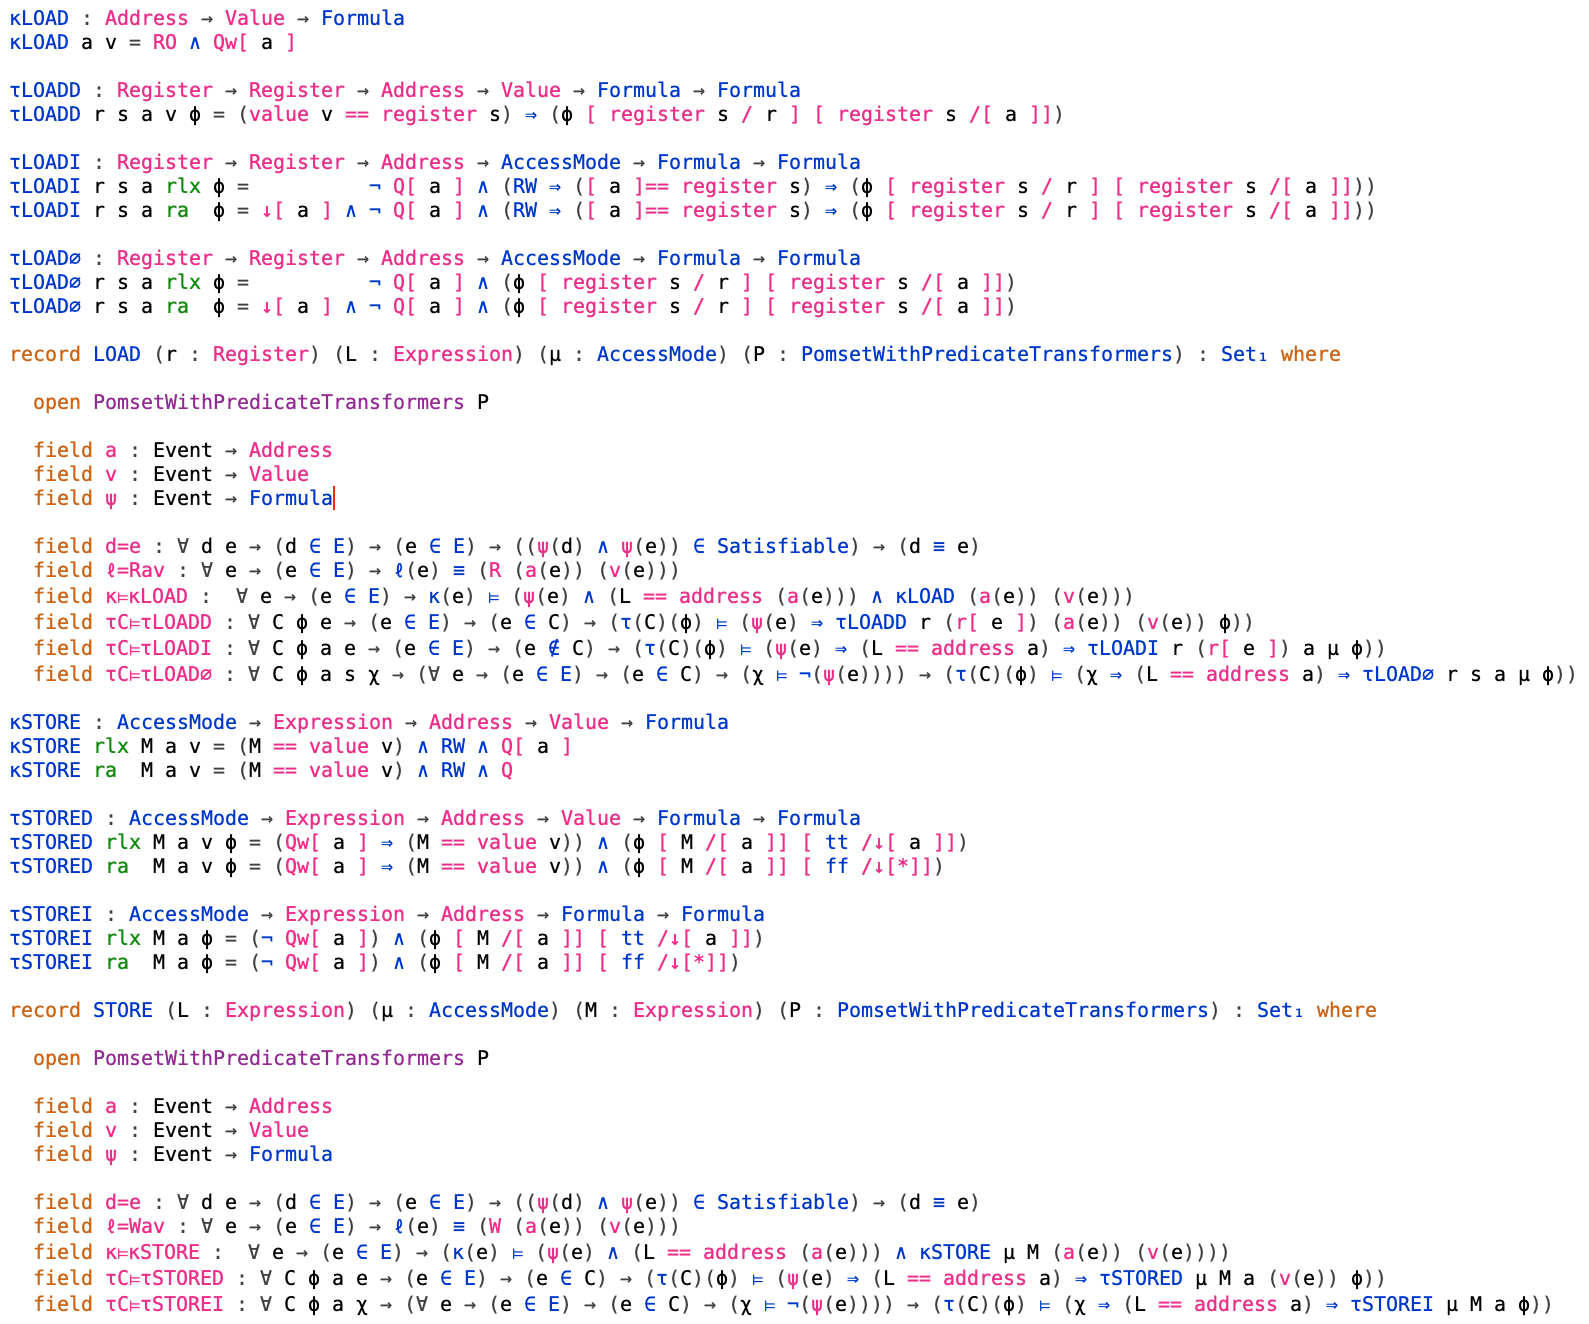
\includegraphics[width=\textwidth]{agda.png}
\end{figure*}

% \section{Future Work}

\citet{DBLP:conf/esop/PaviottiCPWOB20} use step-indexing to account for
loops; we expect that the same approach could be applied here.

% We have presented the first model of relaxed memory that treats sequential
% composition as a first-class citizen. The model builds directly on \jjr{}.

% For sequential composition, parallel composition and the conditional, we
% believe that the definition is \emph{natural}, even \emph{canonical}.
% For stores and loads, instead, the definition in \reffig{fig:no-addr} is a
% Frankenstein's monster of features.  This complexity is \emph{essential},
% however, not just an accident of our poor choices.  Relaxed memory models must
% please many audiences: compiler writers want one thing, hardware designers
% another, and programmers yet another still.  The result is inevitably full of
% compromise.

% Given that \emph{complexity} cannot be eliminated from relaxed memory models,
% the best one can do is attempt to understand its causes.  We have broken the
% problem into seven manageable pieces, discussed throughout
% \textsection\ref{sec:q}--\ref{sec:complications}.  \refdef{def:pomsets-arm}
% summarizes all the features necessary for efficient implementation on
% \armeight{}.  We discuss address calculation, read-modify-write operations
% and fences in the appendix.

% {Logic} is the thread that sews these features together.

% %A unique feature of our model is the centrality of logic: 

% % study each feature in isolation, as a small delta to the base definition
% % given in \textsection\ref{sec:model}.
% % In we studied eight such
% % features.


% % seem staggeringly complex, we argue that this complexity is unavoidable if
% % one wants all the features that it embodies.  By breaking the definition into
% % its constituent parts, we have shown how each of eight


% \subsection*{Acknowledgements}
% % This paper has been greatly improved by the comments of the anonymous reviewers.
% Riely was supported by the National Science Foundation under
% grant No.~CCR-1617175.

% % It is based upon work supported by the National Science Foundation under
% % Grant No. CCR-1617175. Any opinions, findings, and conclusions or
% % recommendations expressed in this material are those of the author and do
% % not necessarily reflect the views of the NSF.}


% \section{Lowering \PwTmcaTITLE{} to Arm}
\label{sec:arm}
For simplicity, we restrict to top-level parallel composition.
% and ignore
% fences\footnote{Fences are not actions in \armeight{}, which complicates the
%   theorem statements.%
%   \app{Is it true? AFAIU, it isn't, they are explicitly used in definition of $\textsc{bob}$.
%     I've just found that Jade prefers to omit them in pictures.}}.
% JWR: I didn't know that!  It's better with them...

\subsection{Arm executions}
\begin{definition}
  An \emph{\armeight{} execution graph}, $\aEG$, is tuple
  $(\aEvs, \labeling, {\rpoloc}, {\rlob})$ such that
  \begin{enumerate}[,label=(\textsc{a}\arabic*),ref=\textsc{a}\arabic*]
  \item $\aEvs\subseteq\AllEvents$ is a set of {events},
  \item $\labeling: \aEvs \fun \Act$ defines a {label} for each event,
  \item ${\rpoloc} \subseteq \aEvs{\times}\aEvs$, is a per-thread, per-location total
    order, capturing \emph{per-location program order},
  \item ${\rlob} \subseteq \aEvs\times\aEvs$, is a per-thread partial order capturing
    \emph{locally-ordered-before}, such that
    \begin{enumerate}
    \item \label{arm-lob-poloc}
      ${\rpoloc} \cup {\rlob}$ is acyclic.
    \end{enumerate}
  \end{enumerate}
\end{definition}

The definition of $\rlob$ is complex.  Comparing with our definition of
sequential composition, it is sufficient to note that $\rlob$ includes
\begin{enumerate}[label=(\textsc{l}\arabic*),ref=\textsc{l}\arabic*]
\item read-write dependencies, required by \ref{seq-kappa},
\item synchronization delay of ${\reorderra}$, required by \ref{seq-le-delays},
\item $\mSC$ access delay of ${\eqreordersc}$, required by \ref{seq-le-delays},
\item write-write and read-to-write coherence delay of ${\eqreorderco}$, required by \ref{seq-le-delays},
\end{enumerate}
and that $\rlob$ does \emph{not} include
\begin{enumerate}[resume,label=(\textsc{l}\arabic*),ref=\textsc{l}\arabic*]
\item \label{lob-rr} \labeltext[above]{}{lob-le}
  read-read control dependencies, required by \ref{seq-kappa},
\item \label{lob-rf}
  write-to-read order of $\rrfx$, required by \ref{pom-rf-le},
\item \label{lob-wr}
  write-to-read coherence delay of ${\eqreorderco}$, required by \ref{seq-le-delays}.
\end{enumerate}

\begin{definition}
  Execution $\aEG$ is
  \emph{$({\rco}, {\rrfx}, {\rgcb})$-valid}, under \emph{External Global
    Consistency} (\EGC{}) if
  \begin{enumerate}[label=(\textsc{a}\arabic*),ref=\textsc{a}\arabic*]
    \setcounter{enumi}{4}
  %\item[\eqref{arm-co}] and \eqref{arm-rf}, as for \EC,
  \item \label{arm-co}
    ${\rco} \subseteq \aEvs\times\aEvs$, is a per-location total order on
    writes, capturing \emph{coherence}, 
  \item \label{arm-rf}
    ${\rrfx} \subseteq \aEvs\times\aEvs$, is a relation, capturing \emph{reads-from}, such that
    \begin{enumerate}
    \item \label{arm-rf-reads}
      ${\rrfx}$ is surjective and injective relation on $\{\aEv\in\aEvs\mid\labeling(\aEv)\;\text{is a}\;\sread\}$,
    \item \label{arm-match}
      if $\bEv\xrfx\aEv$ then $\labeling(\bEv) \rmatches \labeling(\aEv)$,      
    \item \label{arm-local}
      ${\rpoloc} \cup {\rco} \cup {\rrfx} \cup {\rfr}$ is acyclic,
      where $\aEv\xfr\cEv$ if %$(\exists\bEv)$
      $\aEv\xrfxinv\bEv\xco\cEv$, for some $\bEv$,
      % \stepcounter{enumi}
      % \item[] \labeltext[\textsc{a}2]{}{arm-cb}
    \end{enumerate}
    % \item ${\rpoloc} \cup {\rco} \cup {\rrfx} \cup {\rfr}$ is acyclic, where
    %   $\bEv\xfr\aEv$ if $(\exists\cEv)$ $\bEv\xrfxinv\cEv\xco\aEv$,
  \item \label{arm-gcb}
    ${\rgcb}\supseteq\PBR{{\rco}\cup{\rrfx}}$ is a linear order %, capturing \emph{globally completes before}, %$\rcb : % \aEvs\times\aEvs$
    such that 
    \begin{enumerate}%[leftmargin=0pt]
      % \item if $\bEv\xco\aEv$ then $\bEv\xgcb\aEv$,
      % \item if $\bEv\xrfx\aEv$ then $\bEv\xgcb\aEv$,
    \item \label{arm-gcb-blocks}
      if $\bEv\xrfx\aEv$ and $\labeling(\cEv) \rblocks \labeling(\aEv)$ then either $\cEv\xgcb\bEv$ or $\aEv\xgcb\cEv$, 
    \item \label{arm-gcb-lob}
      if $\aEv\xlob\cEv$ then either $\aEv\xgcb\cEv$ or $(\exists\bEv)$
      $\bEv\xrfx\aEv$ and $\bEv\xpoloc\aEv$ but not $\bEv\xlob\cEv$.
    \end{enumerate}
  \end{enumerate}
  
  Execution $\aEG$ is
  \emph{$({\rco}, {\rrfx}, {\rcb})$-valid} under \emph{External Consistency} (\EC{}) if
  \begin{enumerate}[resume,label=(\textsc{a}\arabic*),ref=\textsc{a}\arabic*]
  \item[\eqref{arm-co}] and \eqref{arm-rf}, as for \EGC,
  \item \label{arm-cb}
    ${\rcb}\supseteq\PBR{{\rco}\cup{\rlob}}$ is a linear order %, capturing \emph{completes before}, %$\rcb : % \aEvs\times\aEvs$
    such that if $\bEv\xrfx\aEv$ then either
    \begin{enumerate}%[leftmargin=0pt]
    \item \label{arm-rfe}
      % $\bEv\xcb\aEv$ and $\cEv\rblocks\aEv$ then either $\cEv\xcb\bEv$ or $\aEv\xcb\cEv$, or 
      $\bEv\xcb\aEv$ and if $\labeling(\cEv) \rblocks \labeling(\aEv)$ then either $\cEv\xcb\bEv$ or $\aEv\xcb\cEv$, or
      % $\bEv\xcb\aEv$ and $(\not\exists\cEv)$ such that $\bEv\xcb\cEv\xcb\aEv$ and $\cEv\rblocks\aEv$, or 
    \item \label{arm-rfi}
      $\bEv\xcbinv\aEv$ and $\bEv\xpoloc\aEv$ and $(\not\exists\cEv)$ $\labeling(\cEv) \rblocks \labeling(\aEv)$ and $\bEv\xpoloc\cEv\xpoloc\aEv$.
      % $\bEv\xpoloc\aEv$ and $(\not\exists\cEv)$ such that $\bEv\xpoloc\cEv\xpoloc\aEv$ and $\cEv\rblocks\aEv$.
      % \item if $\bEv\xco\aEv$ then $\bEv\xgcb\aEv$,
      % \item if $\bEv\xrfx\aEv$ then $\bEv\xgcb\aEv$,
      % \item if $\bEv\xrfx\aEv$ and $\cEv\rblocks\aEv$ then either $\cEv\xgcb\bEv$ or $\aEv\xgcb\cEv$,
      % \item if $\bEv\xlob\aEv$ then either $\bEv\xgcb\aEv$ or $(\exists\cEv)$
      %   $\cEv\xrfx\bEv$ and $\cEv\xpoloc\bEv$ but not $\cEv\xlob\aEv$.
    \end{enumerate}
  \end{enumerate}
\end{definition}
\citet{armed} show that \EGC{} and \EC{} are both equivalent to the standard
definition of Arm8.  They explain \EGC{} and \EC{} using the following
example, which is allowed by Arm8.\footnote{We have changed an address
  dependency in the first thread to a data dependency.}
\begin{gather*}
  \PW{x}{1}\SEMI 
  \PR{x}{r}\SEMI
  \PW{y}{r} \PAR
  \PR[\mACQ]{y}{1}\SEMI
  \PR{x}{s}
  \\
  %\tag{\cmark\armeight}
  \hbox{\begin{tikzinline}[node distance=1.5em]
      \event{a}{\DW{x}{1}}{}
      \event{b}{\DR{x}{1}}{right=of a}
      \event{c}{\DW{y}{1}}{right=of b}
      \raevent{d}{\DR[\mACQ]{y}{1}}{right=2.5em of c}
      \event{e}{\DR{x}{0}}{right=of d}
      \rfx{a}{b}
      \lob{b}{c}
      \rfx{c}{d}
      \lob{d}{e}
      \fr[out=-165,in=-15]{e}[above,pos=.375]{a}
    \end{tikzinline}}
\end{gather*}
\EGC{} drops $\rlob$-order in the first thread using \ref{arm-gcb-lob}, since
$\DWP{x}{1}$ is not $\rlob$-ordered before $\DWP{y}{1}$.
\begin{gather*}
  \tag{$\rgcb$}
  \hbox{\begin{tikzinline}[node distance=1.5em]
      \event{a}{\DW{x}{1}}{}
      \event{b}{\DR{x}{1}}{right=of a}
      \event{c}{\DW{y}{1}}{right=of b}
      \raevent{d}{\DR[\mACQ]{y}{1}}{right=2.5em of c}
      \event{e}{\DR{x}{0}}{right=of d}
      \gcbz{a}{b}
      \gcbz{c}{d}
      \gcbz{d}{e}
      \gcbz[out=-165,in=-15]{e}{a}
      % \rfx{a}{b}
      % %\lob{b}{c}
      % \rfx{c}{d}
      % \lob{d}{e}
      % \co[out=-165,in=-15]{e}[above right]{a}
    \end{tikzinline}}
\end{gather*}
\EC{} drops $\rrfx$-order in the first thread using \ref{arm-rfi}.
\begin{gather*}
  \tag{$\rcb$}
  \hbox{\begin{tikzinline}[node distance=1.5em]
      \event{a}{\DW{x}{1}}{}
      \event{b}{\DR{x}{1}}{right=of a}
      \event{c}{\DW{y}{1}}{right=of b}
      \raevent{d}{\DR[\mACQ]{y}{1}}{right=2.5em of c}
      \event{e}{\DR{x}{0}}{right=of d}
      \cbz{b}{c}
      \cbz{c}{d}
      \cbz{d}{e}
      \cbz[out=-165,in=-15]{e}{a}
      % %\rfx{a}{b}
      % \lob{b}{c}
      % \rfx{c}{d}
      % \lob{d}{e}
      % \co[out=-165,in=-15]{e}[above right]{a}
    \end{tikzinline}}
\end{gather*}

\subsection{Lowering \PwTmcaTITLE{1} to Arm}
\label{sec:arm1}

The optimal lowering for \armeight{} is unsound
for \PwTmca{1}.  The optimal lowering maps relaxed access to \LDR/\STR{} and
non-relaxed access to \LDAR/\STLR{} \citep{DBLP:journals/pacmpl/PodkopaevLV19}.
In this section, we consider a suboptimal strategy, which lowers non-relaxed
reads to $(\DMBSY\SEMI\LDAR)$.  Significantly, we retain the optimal lowering
for relaxed access.  In the next section we recover the optimal lowering by
adopting an alternative semantics for \ref{pom-rf-le} and \ref{seq-le-delays}.

To see why the optimal lowering fails, consider the following attempted
execution, where the final values of both $x$ and $y$ are $2$.
\begin{gather*}
  %\taglabel{rfi-coe-coe}
  \PW{x}{2}\SEMI 
  \PR[\mACQ]{x}{r}\SEMI
  \PW{y}{r{-}1} \PAR
  \PW{y}{2}\SEMI
  \PW[\mREL]{x}{1}
  %\\
  %\tag{\cmark\armeight}
  % \hbox{\begin{tikzinline}[node distance=1.5em]
  %     \event{a}{\DW{x}{2}}{}
  %     \raevent{b}{\DR[\mACQ]{x}{2}}{right=of a}
  %     \event{c}{\DW{y}{1}}{right=of b}
  %     \event{d}{\DW{y}{2}}{right=2.5em of c}
  %     \raevent{e}{\DW[\mREL]{x}{1}}{right=of d}
  %     \rfi{a}{b}
  %     \bob{b}{c}
  %     \coe{c}{d}
  %     \bob{d}{e}
  %     \coe[out=-165,in=-15]{e}{a}
  %   \end{tikzinline}}
  \\
  \tag{$\rgcb$}
  \hbox{\begin{tikzinline}[node distance=1.5em]
      \event{a}{\DW{x}{2}}{}
      \raevent{b}{\DR[\mACQ]{x}{2}}{right=of a}
      \event{c}{\DW{y}{1}}{right=of b}
      \event{d}{\DW{y}{2}}{right=2.5em of c}
      \raevent{e}{\DW[\mREL]{x}{1}}{right=of d}
      \gcbz{a}{b}
      %\sync{b}{c}
      \gcbz{c}{d}
      \gcbz{d}{e}
      \gcbz[out=-165,in=-15]{e}{a}
    \end{tikzinline}}
  \\
  \tag{$\le$}
  \hbox{\begin{tikzinline}[node distance=1.5em]
      \event{a}{\DW{x}{2}}{}
      \raevent{b}{\DR[\mACQ]{x}{2}}{right=of a}
      \event{c}{\DW{y}{1}}{right=of b}
      \event{d}{\DW{y}{2}}{right=2.5em of c}
      \raevent{e}{\DW[\mREL]{x}{1}}{right=of d}
      \rf{a}{b}
      \sync{b}{c}
      \wk{c}{d}
      \sync{d}{e}
      \wk[out=-165,in=-15]{e}{a}
    \end{tikzinline}}
\end{gather*}
This attempted execution is allowed by \armeight, but disallowed by our
semantics.

If the read of $x$ in the execution above is changed from acquiring to
relaxed, then our semantics allows the $\rgcb$ execution, using the independent case
for the read and satisfying the precondition of $\DWP{y}{1}$ by prepending
$\DWP{x}{2}$.  It may be tempting, therefore, to adopt a strategy of
\emph{downgrading} acquires in certain cases.  Unfortunately, it is not
possible to do this locally without invalidating important idioms such as
publication.  For example, consider that $\DRP[\mRA]{x}{1}$ is \emph{not} possible for
the second thread in the following attempted execution, due to publication of
$\DWP{x}{2}$ via $y$:
\begin{gather*}
  \PW{x}{\PR{x}{}+1}\SEMI
  \PW[\mREL]{y}{1}
  \PAR
  \PW{x}{1}\SEMI
  \IF{\PR[\mACQ]{y}{}\AND\PR[\mACQ]{x}{}}\THEN
  \PR{z}{s}
  \FI
  \PAR
  \PW{z}{1}\SEMI
  \PW[\mREL]{x}{1}
  \\
  \hbox{\begin{tikzinline}[node distance=1.5em]
      \event{b1}{\DR{x}{1}}{}
      \event{b2}{\DW{x}{2}}{right=of b1}
      \raevent{b3}{\DW[\mREL]{y}{1}}{right=of b2}
      \po{b1}{b2}
      \sync{b2}{b3}
      \event{a1}{\DW{x}{1}}{right=3em of b3}
      \raevent{a2}{\DR[\mACQ]{y}{1}}{right=of a1}
      \raevent{a3}{\DR[\mACQ]{x}{1}}{right=of a2}
      \event{a4}{\DR{z}{0}}{right=of a3}
      \sync{a2}{a3}
      \sync{a3}{a4}
      \event{c1}{\DW{z}{1}}{right=3em of a4}
      \raevent{c2}{\DW[\mREL]{x}{1}}{right=of c1}
      \sync{c1}{c2}
      \rf[out=-165,in=-15]{a1}{b1}
      \rf[out=15,in=165]{b3}{a2}
      \rf[out=-165,in=-15]{c2}{a3}
      \wk{a4}{c1}
    \end{tikzinline}}
\end{gather*}
Instead, if the read of $x$ is relaxed, then the publication via $y$ fails,
and $\DRP{x}{1}$ in the second thread is possible.
\begin{gather*}
  \hbox{\begin{tikzinline}[node distance=1.5em]
      \event{b1}{\DR{x}{1}}{}
      \event{b2}{\DW{x}{2}}{right=of b1}
      \raevent{b3}{\DW[\mREL]{y}{1}}{right=of b2}
      \po{b1}{b2}
      \sync{b2}{b3}
      \event{a1}{\DW{x}{1}}{right=3em of b3}
      \raevent{a2}{\DR[\mACQ]{y}{1}}{right=of a1}
      \event{a3}{\DR{x}{1}}{right=of a2}
      % \raevent{a3}{\DR[\mACQ]{x}{1}}{right=of a2}
      \event{a4}{\DR{z}{0}}{right=of a3}
      \sync{a2}{a3}
      \sync[out=15,in=165]{a2}{a4}
      \event{c1}{\DW{z}{1}}{right=3em of a4}
      \raevent{c2}{\DW[\mREL]{x}{1}}{right=of c1}
      \sync{c1}{c2}
      \rf[out=-165,in=-15]{a1}{b1}
      \rf[out=15,in=165]{b3}{a2}
      \rf[out=-165,in=-15]{c2}{a3}
      \wk{a4}{c1}
    \end{tikzinline}}
\end{gather*}

Using the suboptimal lowering for acquiring reads, our semantics is sound for
Arm.  The proof uses the characterization of Arm using \EGC{}.

\begin{theorem}
  \label{thm:egc}
  Suppose $\aEG_1$ is $({\rco_1}, {\rrfx_1}, {\rgcb_1})$-valid for $\aCmd$
  under the suboptimal lowering that maps non-relaxed reads to
  $(\DMBSY\SEMI\LDAR)$.  Then there is a top-level pomset
  $\aPS_2\in\semrr{\aCmd}$ such that $\aEvs_2=\aEvs_1$,
  $\labeling_2=\labeling_1$, ${\rrfx_2}={\rrfx_1}$, and ${\le_2}={\rgcb_1}$.

  \vspace{-.5\baselineskip}
  \begin{proof}
    First, we establish some lemmas about \armeight.
    
    \vspace{-.5\baselineskip}
    \begin{lemma}
      \label{lemma:fr1}
      Suppose $\aEG$ is $({\rco}, {\rrfx}, {\rgcb})$-valid.  Then
      ${\rgcb}\supseteq{\rfr}$.

      \vspace{-.5\baselineskip}
      \begin{proof}
        Using the definition of ${\rfr}$ from \ref{arm-local}, we have
        $\aEv\xrfxinv\bEv\xco\cEv$, and therefore $\labeling(\cEv)$ blocks
        $\labeling(\aEv)$.    
        Applying \ref{arm-gcb-blocks}, we have that either $\cEv\xgcb\bEv$ or $\aEv\xgcb\cEv$.
        Since $\rgcb$ includes $\rco$, we have $\bEv\xgcb\cEv$, and therefore it
        must be that $\aEv\xgcb\cEv$.
      \end{proof}
    \end{lemma}
    
    \begin{lemma}
      \label{lemma:wr}
      Suppose $\aEG$ is $({\rco}, {\rrfx}, {\rgcb})$-valid and
      $\cEv\xpoloc\aEv$, where $\labeling(\cEv)\rblocks\labeling(\aEv)$.
      Then $\cEv\xgcb\aEv$.
      %$\labeling(\cEv)=\DWP{x}{}$ and $\labeling(\aEv)=\DRP{x}{}$.

      \vspace{-.5\baselineskip}
      \begin{proof}
        By way of contradiction, assume $\aEv\xgcb\cEv$.  If $\cEv\xrfx\aEv$
        then by \ref{arm-gcb} we must also have $\cEv\xgcb\aEv$,
        contradicting the assumption that $\rgcb$ is a total order.
        %
        Otherwise that there is some $\bEv\neq\cEv$ such that
        $\bEv\xrfx\aEv$, and therefore $\bEv\xgcb\aEv$.  By transitivity,
        $\bEv\xgcb\cEv$.  By the definition of $\rfr$, we have
        $\aEv\xfr\cEv$.  But this contradicts \ref{arm-local}, since
        $\cEv\xpoloc\aEv$.
        %Applying \ref{arm-gcb-blocks}, we have that either $\cEv\xgcb\bEv$ or $\aEv\xgcb\cEv$.
      \end{proof}
    \end{lemma}
    We show that all the order required in the pomset is also required by
    \armeight{}.  \ref{pom-rf-block} holds since ${\rcb_1}$ is consistent with
    ${\rco_1}$ and ${\rfr_1}$.  As noted \ref{lob-le}, $\rlob$ includes the order
    required by \ref{seq-kappa} and \ref{seq-le-delays}.  We need only show
    that the order removed from \ref{arm-gcb-lob} can also be removed from
    the pomset.  In order for \ref{arm-gcb-lob} to remove order from $\aEv$
    to $\cEv$, we must have $\bEv\xrfx\aEv$ and $\bEv\xpoloc\aEv$ but not
    $\bEv\xlob\cEv$.  Because of our suboptimal lowering, it must be that
    $\aEv$ is a relaxed read; otherwise the $\DMBSY$ would require
    $\bEv\xlob\cEv$.  Thus we know that \ref{seq-le-delays} does not require
    order from $\aEv$ to $\cEv$.  By chaining \ref{read-tau-ind} and
    \ref{write-tau}, any dependence on the read can by satisfied without
    introducing order in \ref{seq-kappa}.
  \end{proof}  
\end{theorem}



% This model compiles correctly to arm using the lowering: Relaxed access is
% implemented using \texttt{ldr}/\texttt{str}, non-relaxed reads using
% \texttt{dmb st}\SEMI\texttt{ldar}, non-relaxed writes using \texttt{stlr},
% acquire fences using \texttt{dmb}.\texttt{ld} and other fences using 
% \texttt{dmb}.\texttt{sy}.
% \begin{align*}
%   \low{\PW[\gemode\mREL]{\REF{\aReg}}{\bReg}} &= \texttt{stlr}\;\bReg,\REF{\aReg}
%   &
%   \low{\PR[\mRLX]{\REF{\aReg}}{\bReg}} &= \texttt{ldr}\;\bReg,\REF{\aReg}
%   \\
%   \low{\PW[\mRLX]{\REF{\aReg}}{\bReg}} &= \texttt{str}\;\bReg,\REF{\aReg}
%   &
%   \low{\PR[\gemode\mACQ]{\REF{\aReg}}{\bReg}} &= \texttt{dmb st}\SEMI\texttt{ldar}\;\bReg,\REF{\aReg}
% \end{align*}


\subsection{Lowering \PwTmcaTITLE{2} to Arm}
\label{sec:arm2}


We can achieve optimal lowering for Arm by weakening the semantics of
sequential composition slightly.  In particular, we must lose
\ref{pom-rf-le}, which states that $\bEv\xrfx\aEv$ implies
$\bEv\le\aEv$.  Revisiting the example in the last subsection, we essentially
mimic the \EC{} characterization:
\begin{gather*}
  \PW{x}{2}\SEMI 
  \PR[\mACQ]{x}{r}\SEMI
  \PW{y}{r{-}1} \PAR
  \PW{y}{2}\SEMI
  \PW[\mREL]{x}{1}
  \\
  \tag{$\rcb$}
  \hbox{\begin{tikzinline}[node distance=1.5em]
      \event{a}{\DW{x}{2}}{}
      \raevent{b}{\DR[\mACQ]{x}{2}}{right=of a}
      \event{c}{\DW{y}{1}}{right=of b}
      \event{d}{\DW{y}{2}}{right=2.5em of c}
      \raevent{e}{\DW[\mREL]{x}{1}}{right=of d}
      \rfint{a}{b}
      \cbz{b}{c}
      \cbz{c}{d}
      \cbz{d}{e}
      \cbz[out=-165,in=-15]{e}{a}
    \end{tikzinline}}
\end{gather*}
Here the $\rrfx$ relation \emph{contradicts} order!  We have both
$\DWP{x}{2}\xrfint\DRP[\mACQ]{x}{2}$ and
$\DWP{x}{2}\xcbinv\DRP[\mACQ]{x}{2}$.

% The change to the semantics is small: we weaken the relationship between $\rrfx$
% and $\le$ in \ref{seq-rf-le}.  Rather than ensuring that there is no
% \emph{global} blocker for a sequentially fulfilled read \eqref{seq-rf-le}, we
% require only that there is no \emph{thread-local} blocker \eqref{seq-rf-le-rf}.
% This change both allows and requires us to weaken the definition of
% \emph{delays} to drop write-to-read order from $\eqreorderco$.
% \begin{definition}
%   \label{def:sem:frf}
%   Let $\frf{\semrr{}}$ be defined as for $\semrr{}$ in
%   \refdef{def:semrr}/\reffig{fig:sem}, changing \ref{seq-rf-le} and
%   \ref{seq-le-delays}:
%   \begin{itemize}
%   \item[{\labeltext[\frf{\textsc{s}7b}]{(\frf{\textsc{s}7b})}{seq-rf-le-rf}}]
%     if $\labeling_1(\cEv) \rblocks \labeling_2(\aEv)$ and $\bEv\xrfx\aEv$
%     then $\cEv\le\bEv$,
%   \item[{\labeltext[\frf{\textsc{s}6b}]{(\frf{\textsc{s}6b})}{seq-le-delays-rf}}]
%     if $\labeling_1(\bEv) \rdelaysp \labeling_2(\aEv)$ then $\bEv\le\aEv$,\\
%     where $\rdelayspdef$ replaces $\eqreorderco$ in \refdef{def:actions} of
%     $\rdelaysdef$ by
%     \begin{math}
%       {\reorderlws}
%       =
%       \{(\DW{\aLoc}{}, \DW{\aLoc}{}),\;(\DR{\aLoc}{}, \DW{\aLoc}{})\}
%     \end{math}.
%   \item \textcolor{red}{TODO: I think this should order W->R if there is no
%       rf the other way}
%   \end{itemize}  
% \end{definition}
% The acronym $\textsf{lws}$ is adopted from \armeight.  It stands for
% \emph{Local Write Successor}.


We emphasize that \ref{pom-rf-le} does not hold for $\frf{\semrr{}}$:
 $\bEv\xrfx\aEv$ may not imply $\bEv\le\aEv$ when $\bEv$ and $\aEv$ come
from different sides of a sequential composition.  This means that $\rrfx$
must be verified during pomset construction, rather than post-hoc.  The
following lemma gives a post-hoc verification technique for $\rrfx$, using
program order ($\rpox$).\footnote{It is obvious how to enhance the semantics
  of most operators to define $\rpox$.  When combining pomsets using the
  conditional, the obvious definition of $\rpox$ may result in cycles, since
  $\rpox$-ordered events may coalesce.  In this case we include a separate
  pomset for each way of breaking these $\rpox$ cycles.}
% \begin{example}
%   The obvious definition of $\rpox$ may be cyclic, due to the conditional. 
% \end{example}
\begin{lemma}
  Any $\aPS$ in the image of $\frf{\semrr{}}$ is top-level iff
  for every $\bEv\xrfx\aEv$ either
  \begin{itemize}
  \item external fulfillment: $\bEv\le\aEv$ and if $\labeling(\cEv)$ blocks
    $\labeling(\aEv)$ then either $\cEv\le\bEv$ or $\aEv\le\cEv$, or
  \item internal fulfillment: $\bEv\xpox\aEv$ and $(\not\exists\cEv)$
    $\labeling(\cEv) \rblocks \labeling(\aEv)$ and $\bEv\xpox\cEv\xpox\aEv$.
  \end{itemize}
\end{lemma}
% \begin{enumerate}
% \item[(\textsc{m}7d)]
%   if $\labeling(\cEv) \rblocks \labeling(\aEv)$
%   then $\bEv\xrfx\aEv$ implies $\cEv\le\bEv$.
%   %   if $\bEv\xrfx\aEv$ and $\labeling(\cEv) \rblocks \labeling(\aEv)$ then not $\bEv\le\cEv\xpox\aEv$.
% \end{enumerate}




% It follows from these that 
% \begin{itemize}
% \item if $\bEv\xfr\aEv$ then $\bEv\xgcb\aEv$, where $\bEv\xfr\aEv$ if
%   $(\exists\cEv)$ $\bEv\xrfxinv\cEv\xco\aEv$.
% \end{itemize}
% And therefore
% \begin{itemize}
% \item if $\bEv\xeco\aEv$ then $\bEv\xgcb\aEv$.
% \end{itemize}

\begin{theorem}
  \label{thm:ec}
  Suppose $\aEG_1$ %$(\aEvs_1, \labeling_1, {\rpoloc_1}, {\rlob_1})$
  is \EC-valid for $\aCmd$ via $({\rco_1}, {\rrfx_1}, {\rcb_1})$ and that
  ${\rcb_1}\supseteq{\rfr_1}$.  Then there is a top-level pomset
  $\aPS_2\in\frf{\semrr{\aCmd}}$ such that $\aEvs_2=\aEvs_1$,
  $\labeling_2=\labeling_1$, ${\rrfx_2}={\rrfx_1}$, and ${\le_2}={\rcb_1}$.

  \vspace{-.5\baselineskip}
  \begin{proof}
    We show that all the order required in the pomset is also required by
    \armeight{}.  \ref{pom-rf-block} holds since ${\rcb_1}$ is consistent with
    ${\rco_1}$ and ${\rfr_1}$.  \ref{seq-rf-le-rf} follows from \ref{arm-rfi}.
    As noted \ref{lob-le}, $\rlob$ includes the order required by
    \ref{seq-kappa} and \ref{seq-le-delays-rf}.  
  \end{proof}
\end{theorem}

The generality of \refthm{thm:ec} is not limited by the assumption that
${\rcb_1}\supseteq{\rfr_1}$:
\begin{lemma}
  \label{lemma:fr2}
  Suppose $\aEG$ is \EC-valid via $({\rco}, {\rrfx}, {\rcb})$.  Then there a
  permutation ${\rcbp}$ of ${\rcb}$ such that $\aEG$ is \EC-valid via
  $({\rco}, {\rrfx}, {\rcbp})$ and ${\rcbp}\supseteq{\rfr}$, where ${\rfr}$
  is defined in \ref{arm-local}.

  \vspace{-.5\baselineskip}
  \begin{proof}
    We show that any ${\rcb}$ order that contradicts ${\rfr}$ is incidental.

    By definition of $\rfr$, %$(\exists\bEv)$
    $\aEv\xrfxinv\bEv\xco\cEv$, for some $\bEv$.
    Since ${\rcb}\supseteq{\rco}$, we know that $\bEv\xco\cEv$.

    If \ref{arm-rfe} applies to $\bEv\xrfx\aEv$, then $\aEv\xcb\cEv$, since
    it cannot be that $\cEv\xco\bEv$.

    Suppose \ref{arm-rfi} applies to $\bEv\xrfx\aEv$ and $\cEv$ is from a
    different thread.  Because it is a different thread, we cannot have
    $\aEv\xlob\cEv$, and thus the order in $\rcb$ is incidental.

    Suppose \ref{arm-rfi} applies to $\bEv\xrfx\aEv$ and $\cEv$ is from the
    same thread.  Since $\cEv\xco\bEv$, it cannot be that $\cEv\xpoloc\bEv$,
    using \ref{arm-local}.  It also cannot be that
    $\bEv\xpoloc\cEv\xpoloc\aEv$.  It must be that $\aEv\xpoloc\cEv$.  By
    \ref{arm-lob-poloc}, we cannot have $\aEv\xlob\cEv$, and thus the order
    in $\rcb$ is incidental.
  \end{proof}
\end{lemma}


% Lemma: ${\rpoloc}\cup{\rpre}$ is acyclic.

% Theorem: per-thread essential ${\le}$ $\subseteq$ ${\rpoloc}\cup{\rpre}$.


% Bad example:
% \begin{gather*}
%   \PEXCHG{x}{r}{2}\SEMI 
%   \PR{x}{s}\SEMI
%   \PW{y}{s{-}1} \PAR
%   \PR{y}{r}\SEMI
%   \PW{x}{r}
%   \\
%   \tag{\cmark\armeight}
%   \hbox{\begin{tikzinline}[node distance=1.5em]
%       \event{a}{\DR{x}{1}}{}
%       \event{b}{\DW{x}{2}}{right=of a}
%       \event{c}{\DR{x}{2}}{right=of b}
%       \event{d}{\DW{y}{1}}{right=of c}
%       \event{e}{\DR{y}{1}}{right=3em of d}
%       \event{f}{\DW{x}{1}}{right=of e}
%       \pre{a}{b}
%       \rf{b}{c}
%       \lob{c}{d}
%       \rf{d}{e}
%       \pre{e}{f}
%       \rf[out=-165,in=-15]{f}{a}
%     \end{tikzinline}}
%   % \hbox{\begin{tikzinline}[node distance=1.5em]
%   %   \event{a}{\DR{x}{1}}{}
%   %   \event{b}{\DW{x}{2}}{right=of a}
%   %   \event{c}{\DR{x}{2}}{right=of b}
%   %   \event{d}{\DW{y}{1}}{right=of c}
%   %   \event{e}{\DR{y}{1}}{right=3em of d}
%   %   \event{f}{\DW{x}{1}}{right=of e}
%   %   \rmw{a}{b}
%   %   \rfi{b}{c}
%   %   \dob{c}{d}
%   %   \rfe{d}{e}
%   %   \dob{e}{f}
%   %   \rfe[out=-165,in=-15]{f}{a}
%   % \end{tikzinline}}
%   \\
%   \tag{$\le$}
%   \hbox{\begin{tikzinline}[node distance=1.5em]
%       \event{a}{\DR{x}{1}}{}
%       \event{b}{\DW{x}{2}}{right=of a}
%       \event{c}{\DR{x}{2}}{right=of b}
%       \event{d}{\DW{y}{1}}{right=of c}
%       \event{e}{\DR{y}{1}}{right=3em of d}
%       \event{f}{\DW{x}{1}}{right=of e}
%       \rmw{a}{b}
%       \rf{b}{c}
%       % \po{c}{d}
%       \rf{d}{e}
%       \po{e}{f}
%       \rf[out=-165,in=-15]{f}{a}
%     \end{tikzinline}}
% \end{gather*}



% \clearpage
% \RequirePackage{amssymb}  %% bizarre error previous def of Bbbk if after documentclass
\documentclass[acmsmall,screen]{acmart}\settopmatter{printfolios=true}
\hypersetup{bookmarksnumbered,bookmarksopen=true,bookmarksdepth=3}
\settopmatter{printfolios=true}
\AtEndPreamble{%
  \theoremstyle{acmdefinition}
  \newtheorem{remark}[theorem]{Remark}
  \newtheorem{candidate}[theorem]{Candidate}
  \renewcommand{\theequation}{\fnsymbol{equation}}
}
\bibliographystyle{ACM-Reference-Format}
\citestyle{acmauthoryear}   %% For author/year citations

\setcopyright{rightsretained}
\acmPrice{}
\acmDOI{}
\acmYear{2022}
\copyrightyear{2022}
\acmSubmissionID{}
\acmJournal{PACMPL}
\acmVolume{0}
\acmNumber{POPL}
\acmArticle{0}
\acmMonth{1}
\startPage{1}

\usepackage{macros}
% \showRAfalse
\showSCOPEfalse
\title{The Leaky Semicolon (Supplementary Material)}


\usepackage{xr}
\externaldocument{paper}
\makecounter{Bkappa} \setcounter{Bkappa}{2}
\makecounter{Btau}   \setcounter{Btau}{3}
\makecounter{Bterm}  \setcounter{Bterm}{4}
\begin{document}
\setcounter{page}{31}
\appendix
\noindent
{\LARGE \textsf{\textbf{The Leaky Semicolon (Supplementary Material)}}}
\bigskip

\section{Lowering \PwTmcaTITLE{} to Arm}
\label{sec:arm}
For simplicity, we restrict to top-level parallel composition.
% and ignore
% fences\footnote{Fences are not actions in \armeight{}, which complicates the
%   theorem statements.%
%   \app{Is it true? AFAIU, it isn't, they are explicitly used in definition of $\textsc{bob}$.
%     I've just found that Jade prefers to omit them in pictures.}}.
% JWR: I didn't know that!  It's better with them...

\subsection{Arm executions}
\begin{definition}
  An \emph{\armeight{} execution graph}, $\aEG$, is tuple
  $(\aEvs, \labeling, {\rpoloc}, {\rlob})$ such that
  \begin{enumerate}[,label=(\textsc{a}\arabic*),ref=\textsc{a}\arabic*]
  \item $\aEvs\subseteq\AllEvents$ is a set of {events},
  \item $\labeling: \aEvs \fun \Act$ defines a {label} for each event,
  \item ${\rpoloc} \subseteq \aEvs{\times}\aEvs$, is a per-thread, per-location total
    order, capturing \emph{per-location program order},
  \item ${\rlob} \subseteq \aEvs\times\aEvs$, is a per-thread partial order capturing
    \emph{locally-ordered-before}, such that
    \begin{enumerate}
    \item \label{arm-lob-poloc}
      ${\rpoloc} \cup {\rlob}$ is acyclic.
    \end{enumerate}
  \end{enumerate}
\end{definition}

The definition of $\rlob$ is complex.  Comparing with our definition of
sequential composition, it is sufficient to note that $\rlob$ includes
\begin{enumerate}[label=(\textsc{l}\arabic*),ref=\textsc{l}\arabic*]
\item read-write dependencies, required by \ref{seq-kappa},
\item synchronization delay of ${\reorderra}$, required by \ref{seq-le-delays},
\item $\mSC$ access delay of ${\eqreordersc}$, required by \ref{seq-le-delays},
\item write-write and read-to-write coherence delay of ${\eqreorderco}$, required by \ref{seq-le-delays},
\end{enumerate}
and that $\rlob$ does \emph{not} include
\begin{enumerate}[resume,label=(\textsc{l}\arabic*),ref=\textsc{l}\arabic*]
\item \label{lob-rr} \labeltext[above]{}{lob-le}
  read-read control dependencies, required by \ref{seq-kappa},
\item \label{lob-rf}
  write-to-read order of $\rrfx$, required by \ref{pom-rf-le},
\item \label{lob-wr}
  write-to-read coherence delay of ${\eqreorderco}$, required by \ref{seq-le-delays}.
\end{enumerate}

\begin{definition}
  Execution $\aEG$ is
  \emph{$({\rco}, {\rrfx}, {\rgcb})$-valid}, under \emph{External Global
    Consistency} (\EGC{}) if
  \begin{enumerate}[label=(\textsc{a}\arabic*),ref=\textsc{a}\arabic*]
    \setcounter{enumi}{4}
  %\item[\eqref{arm-co}] and \eqref{arm-rf}, as for \EC,
  \item \label{arm-co}
    ${\rco} \subseteq \aEvs\times\aEvs$, is a per-location total order on
    writes, capturing \emph{coherence}, 
  \item \label{arm-rf}
    ${\rrfx} \subseteq \aEvs\times\aEvs$, is a relation, capturing \emph{reads-from}, such that
    \begin{enumerate}
    \item \label{arm-rf-reads}
      ${\rrfx}$ is surjective and injective relation on $\{\aEv\in\aEvs\mid\labeling(\aEv)\;\text{is a}\;\sread\}$,
    \item \label{arm-match}
      if $\bEv\xrfx\aEv$ then $\labeling(\bEv) \rmatches \labeling(\aEv)$,      
    \item \label{arm-local}
      ${\rpoloc} \cup {\rco} \cup {\rrfx} \cup {\rfr}$ is acyclic,
      where $\aEv\xfr\cEv$ if %$(\exists\bEv)$
      $\aEv\xrfxinv\bEv\xco\cEv$, for some $\bEv$,
      % \stepcounter{enumi}
      % \item[] \labeltext[\textsc{a}2]{}{arm-cb}
    \end{enumerate}
    % \item ${\rpoloc} \cup {\rco} \cup {\rrfx} \cup {\rfr}$ is acyclic, where
    %   $\bEv\xfr\aEv$ if $(\exists\cEv)$ $\bEv\xrfxinv\cEv\xco\aEv$,
  \item \label{arm-gcb}
    ${\rgcb}\supseteq\PBR{{\rco}\cup{\rrfx}}$ is a linear order %, capturing \emph{globally completes before}, %$\rcb : % \aEvs\times\aEvs$
    such that 
    \begin{enumerate}%[leftmargin=0pt]
      % \item if $\bEv\xco\aEv$ then $\bEv\xgcb\aEv$,
      % \item if $\bEv\xrfx\aEv$ then $\bEv\xgcb\aEv$,
    \item \label{arm-gcb-blocks}
      if $\bEv\xrfx\aEv$ and $\labeling(\cEv) \rblocks \labeling(\aEv)$ then either $\cEv\xgcb\bEv$ or $\aEv\xgcb\cEv$, 
    \item \label{arm-gcb-lob}
      if $\aEv\xlob\cEv$ then either $\aEv\xgcb\cEv$ or $(\exists\bEv)$
      $\bEv\xrfx\aEv$ and $\bEv\xpoloc\aEv$ but not $\bEv\xlob\cEv$.
    \end{enumerate}
  \end{enumerate}
  
  Execution $\aEG$ is
  \emph{$({\rco}, {\rrfx}, {\rcb})$-valid} under \emph{External Consistency} (\EC{}) if
  \begin{enumerate}[resume,label=(\textsc{a}\arabic*),ref=\textsc{a}\arabic*]
  \item[\eqref{arm-co}] and \eqref{arm-rf}, as for \EGC,
  \item \label{arm-cb}
    ${\rcb}\supseteq\PBR{{\rco}\cup{\rlob}}$ is a linear order %, capturing \emph{completes before}, %$\rcb : % \aEvs\times\aEvs$
    such that if $\bEv\xrfx\aEv$ then either
    \begin{enumerate}%[leftmargin=0pt]
    \item \label{arm-rfe}
      % $\bEv\xcb\aEv$ and $\cEv\rblocks\aEv$ then either $\cEv\xcb\bEv$ or $\aEv\xcb\cEv$, or 
      $\bEv\xcb\aEv$ and if $\labeling(\cEv) \rblocks \labeling(\aEv)$ then either $\cEv\xcb\bEv$ or $\aEv\xcb\cEv$, or
      % $\bEv\xcb\aEv$ and $(\not\exists\cEv)$ such that $\bEv\xcb\cEv\xcb\aEv$ and $\cEv\rblocks\aEv$, or 
    \item \label{arm-rfi}
      $\bEv\xcbinv\aEv$ and $\bEv\xpoloc\aEv$ and $(\not\exists\cEv)$ $\labeling(\cEv) \rblocks \labeling(\aEv)$ and $\bEv\xpoloc\cEv\xpoloc\aEv$.
      % $\bEv\xpoloc\aEv$ and $(\not\exists\cEv)$ such that $\bEv\xpoloc\cEv\xpoloc\aEv$ and $\cEv\rblocks\aEv$.
      % \item if $\bEv\xco\aEv$ then $\bEv\xgcb\aEv$,
      % \item if $\bEv\xrfx\aEv$ then $\bEv\xgcb\aEv$,
      % \item if $\bEv\xrfx\aEv$ and $\cEv\rblocks\aEv$ then either $\cEv\xgcb\bEv$ or $\aEv\xgcb\cEv$,
      % \item if $\bEv\xlob\aEv$ then either $\bEv\xgcb\aEv$ or $(\exists\cEv)$
      %   $\cEv\xrfx\bEv$ and $\cEv\xpoloc\bEv$ but not $\cEv\xlob\aEv$.
    \end{enumerate}
  \end{enumerate}
\end{definition}
\citet{armed} show that \EGC{} and \EC{} are both equivalent to the standard
definition of Arm8.  They explain \EGC{} and \EC{} using the following
example, which is allowed by Arm8.\footnote{We have changed an address
  dependency in the first thread to a data dependency.}
\begin{gather*}
  \PW{x}{1}\SEMI 
  \PR{x}{r}\SEMI
  \PW{y}{r} \PAR
  \PR[\mACQ]{y}{1}\SEMI
  \PR{x}{s}
  \\
  %\tag{\cmark\armeight}
  \hbox{\begin{tikzinline}[node distance=1.5em]
      \event{a}{\DW{x}{1}}{}
      \event{b}{\DR{x}{1}}{right=of a}
      \event{c}{\DW{y}{1}}{right=of b}
      \raevent{d}{\DR[\mACQ]{y}{1}}{right=2.5em of c}
      \event{e}{\DR{x}{0}}{right=of d}
      \rfx{a}{b}
      \lob{b}{c}
      \rfx{c}{d}
      \lob{d}{e}
      \fr[out=-165,in=-15]{e}[above,pos=.375]{a}
    \end{tikzinline}}
\end{gather*}
\EGC{} drops $\rlob$-order in the first thread using \ref{arm-gcb-lob}, since
$\DWP{x}{1}$ is not $\rlob$-ordered before $\DWP{y}{1}$.
\begin{gather*}
  \tag{$\rgcb$}
  \hbox{\begin{tikzinline}[node distance=1.5em]
      \event{a}{\DW{x}{1}}{}
      \event{b}{\DR{x}{1}}{right=of a}
      \event{c}{\DW{y}{1}}{right=of b}
      \raevent{d}{\DR[\mACQ]{y}{1}}{right=2.5em of c}
      \event{e}{\DR{x}{0}}{right=of d}
      \gcbz{a}{b}
      \gcbz{c}{d}
      \gcbz{d}{e}
      \gcbz[out=-165,in=-15]{e}{a}
      % \rfx{a}{b}
      % %\lob{b}{c}
      % \rfx{c}{d}
      % \lob{d}{e}
      % \co[out=-165,in=-15]{e}[above right]{a}
    \end{tikzinline}}
\end{gather*}
\EC{} drops $\rrfx$-order in the first thread using \ref{arm-rfi}.
\begin{gather*}
  \tag{$\rcb$}
  \hbox{\begin{tikzinline}[node distance=1.5em]
      \event{a}{\DW{x}{1}}{}
      \event{b}{\DR{x}{1}}{right=of a}
      \event{c}{\DW{y}{1}}{right=of b}
      \raevent{d}{\DR[\mACQ]{y}{1}}{right=2.5em of c}
      \event{e}{\DR{x}{0}}{right=of d}
      \cbz{b}{c}
      \cbz{c}{d}
      \cbz{d}{e}
      \cbz[out=-165,in=-15]{e}{a}
      % %\rfx{a}{b}
      % \lob{b}{c}
      % \rfx{c}{d}
      % \lob{d}{e}
      % \co[out=-165,in=-15]{e}[above right]{a}
    \end{tikzinline}}
\end{gather*}

\subsection{Lowering \PwTmcaTITLE{1} to Arm}
\label{sec:arm1}

The optimal lowering for \armeight{} is unsound
for \PwTmca{1}.  The optimal lowering maps relaxed access to \LDR/\STR{} and
non-relaxed access to \LDAR/\STLR{} \citep{DBLP:journals/pacmpl/PodkopaevLV19}.
In this section, we consider a suboptimal strategy, which lowers non-relaxed
reads to $(\DMBSY\SEMI\LDAR)$.  Significantly, we retain the optimal lowering
for relaxed access.  In the next section we recover the optimal lowering by
adopting an alternative semantics for \ref{pom-rf-le} and \ref{seq-le-delays}.

To see why the optimal lowering fails, consider the following attempted
execution, where the final values of both $x$ and $y$ are $2$.
\begin{gather*}
  %\taglabel{rfi-coe-coe}
  \PW{x}{2}\SEMI 
  \PR[\mACQ]{x}{r}\SEMI
  \PW{y}{r{-}1} \PAR
  \PW{y}{2}\SEMI
  \PW[\mREL]{x}{1}
  %\\
  %\tag{\cmark\armeight}
  % \hbox{\begin{tikzinline}[node distance=1.5em]
  %     \event{a}{\DW{x}{2}}{}
  %     \raevent{b}{\DR[\mACQ]{x}{2}}{right=of a}
  %     \event{c}{\DW{y}{1}}{right=of b}
  %     \event{d}{\DW{y}{2}}{right=2.5em of c}
  %     \raevent{e}{\DW[\mREL]{x}{1}}{right=of d}
  %     \rfi{a}{b}
  %     \bob{b}{c}
  %     \coe{c}{d}
  %     \bob{d}{e}
  %     \coe[out=-165,in=-15]{e}{a}
  %   \end{tikzinline}}
  \\
  \tag{$\rgcb$}
  \hbox{\begin{tikzinline}[node distance=1.5em]
      \event{a}{\DW{x}{2}}{}
      \raevent{b}{\DR[\mACQ]{x}{2}}{right=of a}
      \event{c}{\DW{y}{1}}{right=of b}
      \event{d}{\DW{y}{2}}{right=2.5em of c}
      \raevent{e}{\DW[\mREL]{x}{1}}{right=of d}
      \gcbz{a}{b}
      %\sync{b}{c}
      \gcbz{c}{d}
      \gcbz{d}{e}
      \gcbz[out=-165,in=-15]{e}{a}
    \end{tikzinline}}
  \\
  \tag{$\le$}
  \hbox{\begin{tikzinline}[node distance=1.5em]
      \event{a}{\DW{x}{2}}{}
      \raevent{b}{\DR[\mACQ]{x}{2}}{right=of a}
      \event{c}{\DW{y}{1}}{right=of b}
      \event{d}{\DW{y}{2}}{right=2.5em of c}
      \raevent{e}{\DW[\mREL]{x}{1}}{right=of d}
      \rf{a}{b}
      \sync{b}{c}
      \wk{c}{d}
      \sync{d}{e}
      \wk[out=-165,in=-15]{e}{a}
    \end{tikzinline}}
\end{gather*}
This attempted execution is allowed by \armeight, but disallowed by our
semantics.

If the read of $x$ in the execution above is changed from acquiring to
relaxed, then our semantics allows the $\rgcb$ execution, using the independent case
for the read and satisfying the precondition of $\DWP{y}{1}$ by prepending
$\DWP{x}{2}$.  It may be tempting, therefore, to adopt a strategy of
\emph{downgrading} acquires in certain cases.  Unfortunately, it is not
possible to do this locally without invalidating important idioms such as
publication.  For example, consider that $\DRP[\mRA]{x}{1}$ is \emph{not} possible for
the second thread in the following attempted execution, due to publication of
$\DWP{x}{2}$ via $y$:
\begin{gather*}
  \PW{x}{\PR{x}{}+1}\SEMI
  \PW[\mREL]{y}{1}
  \PAR
  \PW{x}{1}\SEMI
  \IF{\PR[\mACQ]{y}{}\AND\PR[\mACQ]{x}{}}\THEN
  \PR{z}{s}
  \FI
  \PAR
  \PW{z}{1}\SEMI
  \PW[\mREL]{x}{1}
  \\
  \hbox{\begin{tikzinline}[node distance=1.5em]
      \event{b1}{\DR{x}{1}}{}
      \event{b2}{\DW{x}{2}}{right=of b1}
      \raevent{b3}{\DW[\mREL]{y}{1}}{right=of b2}
      \po{b1}{b2}
      \sync{b2}{b3}
      \event{a1}{\DW{x}{1}}{right=3em of b3}
      \raevent{a2}{\DR[\mACQ]{y}{1}}{right=of a1}
      \raevent{a3}{\DR[\mACQ]{x}{1}}{right=of a2}
      \event{a4}{\DR{z}{0}}{right=of a3}
      \sync{a2}{a3}
      \sync{a3}{a4}
      \event{c1}{\DW{z}{1}}{right=3em of a4}
      \raevent{c2}{\DW[\mREL]{x}{1}}{right=of c1}
      \sync{c1}{c2}
      \rf[out=-165,in=-15]{a1}{b1}
      \rf[out=15,in=165]{b3}{a2}
      \rf[out=-165,in=-15]{c2}{a3}
      \wk{a4}{c1}
    \end{tikzinline}}
\end{gather*}
Instead, if the read of $x$ is relaxed, then the publication via $y$ fails,
and $\DRP{x}{1}$ in the second thread is possible.
\begin{gather*}
  \hbox{\begin{tikzinline}[node distance=1.5em]
      \event{b1}{\DR{x}{1}}{}
      \event{b2}{\DW{x}{2}}{right=of b1}
      \raevent{b3}{\DW[\mREL]{y}{1}}{right=of b2}
      \po{b1}{b2}
      \sync{b2}{b3}
      \event{a1}{\DW{x}{1}}{right=3em of b3}
      \raevent{a2}{\DR[\mACQ]{y}{1}}{right=of a1}
      \event{a3}{\DR{x}{1}}{right=of a2}
      % \raevent{a3}{\DR[\mACQ]{x}{1}}{right=of a2}
      \event{a4}{\DR{z}{0}}{right=of a3}
      \sync{a2}{a3}
      \sync[out=15,in=165]{a2}{a4}
      \event{c1}{\DW{z}{1}}{right=3em of a4}
      \raevent{c2}{\DW[\mREL]{x}{1}}{right=of c1}
      \sync{c1}{c2}
      \rf[out=-165,in=-15]{a1}{b1}
      \rf[out=15,in=165]{b3}{a2}
      \rf[out=-165,in=-15]{c2}{a3}
      \wk{a4}{c1}
    \end{tikzinline}}
\end{gather*}

Using the suboptimal lowering for acquiring reads, our semantics is sound for
Arm.  The proof uses the characterization of Arm using \EGC{}.

\begin{theorem}
  \label{thm:egc}
  Suppose $\aEG_1$ is $({\rco_1}, {\rrfx_1}, {\rgcb_1})$-valid for $\aCmd$
  under the suboptimal lowering that maps non-relaxed reads to
  $(\DMBSY\SEMI\LDAR)$.  Then there is a top-level pomset
  $\aPS_2\in\semrr{\aCmd}$ such that $\aEvs_2=\aEvs_1$,
  $\labeling_2=\labeling_1$, ${\rrfx_2}={\rrfx_1}$, and ${\le_2}={\rgcb_1}$.

  \vspace{-.5\baselineskip}
  \begin{proof}
    First, we establish some lemmas about \armeight.
    
    \vspace{-.5\baselineskip}
    \begin{lemma}
      \label{lemma:fr1}
      Suppose $\aEG$ is $({\rco}, {\rrfx}, {\rgcb})$-valid.  Then
      ${\rgcb}\supseteq{\rfr}$.

      \vspace{-.5\baselineskip}
      \begin{proof}
        Using the definition of ${\rfr}$ from \ref{arm-local}, we have
        $\aEv\xrfxinv\bEv\xco\cEv$, and therefore $\labeling(\cEv)$ blocks
        $\labeling(\aEv)$.    
        Applying \ref{arm-gcb-blocks}, we have that either $\cEv\xgcb\bEv$ or $\aEv\xgcb\cEv$.
        Since $\rgcb$ includes $\rco$, we have $\bEv\xgcb\cEv$, and therefore it
        must be that $\aEv\xgcb\cEv$.
      \end{proof}
    \end{lemma}
    
    \begin{lemma}
      \label{lemma:wr}
      Suppose $\aEG$ is $({\rco}, {\rrfx}, {\rgcb})$-valid and
      $\cEv\xpoloc\aEv$, where $\labeling(\cEv)\rblocks\labeling(\aEv)$.
      Then $\cEv\xgcb\aEv$.
      %$\labeling(\cEv)=\DWP{x}{}$ and $\labeling(\aEv)=\DRP{x}{}$.

      \vspace{-.5\baselineskip}
      \begin{proof}
        By way of contradiction, assume $\aEv\xgcb\cEv$.  If $\cEv\xrfx\aEv$
        then by \ref{arm-gcb} we must also have $\cEv\xgcb\aEv$,
        contradicting the assumption that $\rgcb$ is a total order.
        %
        Otherwise that there is some $\bEv\neq\cEv$ such that
        $\bEv\xrfx\aEv$, and therefore $\bEv\xgcb\aEv$.  By transitivity,
        $\bEv\xgcb\cEv$.  By the definition of $\rfr$, we have
        $\aEv\xfr\cEv$.  But this contradicts \ref{arm-local}, since
        $\cEv\xpoloc\aEv$.
        %Applying \ref{arm-gcb-blocks}, we have that either $\cEv\xgcb\bEv$ or $\aEv\xgcb\cEv$.
      \end{proof}
    \end{lemma}
    We show that all the order required in the pomset is also required by
    \armeight{}.  \ref{pom-rf-block} holds since ${\rcb_1}$ is consistent with
    ${\rco_1}$ and ${\rfr_1}$.  As noted \ref{lob-le}, $\rlob$ includes the order
    required by \ref{seq-kappa} and \ref{seq-le-delays}.  We need only show
    that the order removed from \ref{arm-gcb-lob} can also be removed from
    the pomset.  In order for \ref{arm-gcb-lob} to remove order from $\aEv$
    to $\cEv$, we must have $\bEv\xrfx\aEv$ and $\bEv\xpoloc\aEv$ but not
    $\bEv\xlob\cEv$.  Because of our suboptimal lowering, it must be that
    $\aEv$ is a relaxed read; otherwise the $\DMBSY$ would require
    $\bEv\xlob\cEv$.  Thus we know that \ref{seq-le-delays} does not require
    order from $\aEv$ to $\cEv$.  By chaining \ref{read-tau-ind} and
    \ref{write-tau}, any dependence on the read can by satisfied without
    introducing order in \ref{seq-kappa}.
  \end{proof}  
\end{theorem}



% This model compiles correctly to arm using the lowering: Relaxed access is
% implemented using \texttt{ldr}/\texttt{str}, non-relaxed reads using
% \texttt{dmb st}\SEMI\texttt{ldar}, non-relaxed writes using \texttt{stlr},
% acquire fences using \texttt{dmb}.\texttt{ld} and other fences using 
% \texttt{dmb}.\texttt{sy}.
% \begin{align*}
%   \low{\PW[\gemode\mREL]{\REF{\aReg}}{\bReg}} &= \texttt{stlr}\;\bReg,\REF{\aReg}
%   &
%   \low{\PR[\mRLX]{\REF{\aReg}}{\bReg}} &= \texttt{ldr}\;\bReg,\REF{\aReg}
%   \\
%   \low{\PW[\mRLX]{\REF{\aReg}}{\bReg}} &= \texttt{str}\;\bReg,\REF{\aReg}
%   &
%   \low{\PR[\gemode\mACQ]{\REF{\aReg}}{\bReg}} &= \texttt{dmb st}\SEMI\texttt{ldar}\;\bReg,\REF{\aReg}
% \end{align*}


\subsection{Lowering \PwTmcaTITLE{2} to Arm}
\label{sec:arm2}


We can achieve optimal lowering for Arm by weakening the semantics of
sequential composition slightly.  In particular, we must lose
\ref{pom-rf-le}, which states that $\bEv\xrfx\aEv$ implies
$\bEv\le\aEv$.  Revisiting the example in the last subsection, we essentially
mimic the \EC{} characterization:
\begin{gather*}
  \PW{x}{2}\SEMI 
  \PR[\mACQ]{x}{r}\SEMI
  \PW{y}{r{-}1} \PAR
  \PW{y}{2}\SEMI
  \PW[\mREL]{x}{1}
  \\
  \tag{$\rcb$}
  \hbox{\begin{tikzinline}[node distance=1.5em]
      \event{a}{\DW{x}{2}}{}
      \raevent{b}{\DR[\mACQ]{x}{2}}{right=of a}
      \event{c}{\DW{y}{1}}{right=of b}
      \event{d}{\DW{y}{2}}{right=2.5em of c}
      \raevent{e}{\DW[\mREL]{x}{1}}{right=of d}
      \rfint{a}{b}
      \cbz{b}{c}
      \cbz{c}{d}
      \cbz{d}{e}
      \cbz[out=-165,in=-15]{e}{a}
    \end{tikzinline}}
\end{gather*}
Here the $\rrfx$ relation \emph{contradicts} order!  We have both
$\DWP{x}{2}\xrfint\DRP[\mACQ]{x}{2}$ and
$\DWP{x}{2}\xcbinv\DRP[\mACQ]{x}{2}$.

% The change to the semantics is small: we weaken the relationship between $\rrfx$
% and $\le$ in \ref{seq-rf-le}.  Rather than ensuring that there is no
% \emph{global} blocker for a sequentially fulfilled read \eqref{seq-rf-le}, we
% require only that there is no \emph{thread-local} blocker \eqref{seq-rf-le-rf}.
% This change both allows and requires us to weaken the definition of
% \emph{delays} to drop write-to-read order from $\eqreorderco$.
% \begin{definition}
%   \label{def:sem:frf}
%   Let $\frf{\semrr{}}$ be defined as for $\semrr{}$ in
%   \refdef{def:semrr}/\reffig{fig:sem}, changing \ref{seq-rf-le} and
%   \ref{seq-le-delays}:
%   \begin{itemize}
%   \item[{\labeltext[\frf{\textsc{s}7b}]{(\frf{\textsc{s}7b})}{seq-rf-le-rf}}]
%     if $\labeling_1(\cEv) \rblocks \labeling_2(\aEv)$ and $\bEv\xrfx\aEv$
%     then $\cEv\le\bEv$,
%   \item[{\labeltext[\frf{\textsc{s}6b}]{(\frf{\textsc{s}6b})}{seq-le-delays-rf}}]
%     if $\labeling_1(\bEv) \rdelaysp \labeling_2(\aEv)$ then $\bEv\le\aEv$,\\
%     where $\rdelayspdef$ replaces $\eqreorderco$ in \refdef{def:actions} of
%     $\rdelaysdef$ by
%     \begin{math}
%       {\reorderlws}
%       =
%       \{(\DW{\aLoc}{}, \DW{\aLoc}{}),\;(\DR{\aLoc}{}, \DW{\aLoc}{})\}
%     \end{math}.
%   \item \textcolor{red}{TODO: I think this should order W->R if there is no
%       rf the other way}
%   \end{itemize}  
% \end{definition}
% The acronym $\textsf{lws}$ is adopted from \armeight.  It stands for
% \emph{Local Write Successor}.


We emphasize that \ref{pom-rf-le} does not hold for $\frf{\semrr{}}$:
 $\bEv\xrfx\aEv$ may not imply $\bEv\le\aEv$ when $\bEv$ and $\aEv$ come
from different sides of a sequential composition.  This means that $\rrfx$
must be verified during pomset construction, rather than post-hoc.  The
following lemma gives a post-hoc verification technique for $\rrfx$, using
program order ($\rpox$).\footnote{It is obvious how to enhance the semantics
  of most operators to define $\rpox$.  When combining pomsets using the
  conditional, the obvious definition of $\rpox$ may result in cycles, since
  $\rpox$-ordered events may coalesce.  In this case we include a separate
  pomset for each way of breaking these $\rpox$ cycles.}
% \begin{example}
%   The obvious definition of $\rpox$ may be cyclic, due to the conditional. 
% \end{example}
\begin{lemma}
  Any $\aPS$ in the image of $\frf{\semrr{}}$ is top-level iff
  for every $\bEv\xrfx\aEv$ either
  \begin{itemize}
  \item external fulfillment: $\bEv\le\aEv$ and if $\labeling(\cEv)$ blocks
    $\labeling(\aEv)$ then either $\cEv\le\bEv$ or $\aEv\le\cEv$, or
  \item internal fulfillment: $\bEv\xpox\aEv$ and $(\not\exists\cEv)$
    $\labeling(\cEv) \rblocks \labeling(\aEv)$ and $\bEv\xpox\cEv\xpox\aEv$.
  \end{itemize}
\end{lemma}
% \begin{enumerate}
% \item[(\textsc{m}7d)]
%   if $\labeling(\cEv) \rblocks \labeling(\aEv)$
%   then $\bEv\xrfx\aEv$ implies $\cEv\le\bEv$.
%   %   if $\bEv\xrfx\aEv$ and $\labeling(\cEv) \rblocks \labeling(\aEv)$ then not $\bEv\le\cEv\xpox\aEv$.
% \end{enumerate}




% It follows from these that 
% \begin{itemize}
% \item if $\bEv\xfr\aEv$ then $\bEv\xgcb\aEv$, where $\bEv\xfr\aEv$ if
%   $(\exists\cEv)$ $\bEv\xrfxinv\cEv\xco\aEv$.
% \end{itemize}
% And therefore
% \begin{itemize}
% \item if $\bEv\xeco\aEv$ then $\bEv\xgcb\aEv$.
% \end{itemize}

\begin{theorem}
  \label{thm:ec}
  Suppose $\aEG_1$ %$(\aEvs_1, \labeling_1, {\rpoloc_1}, {\rlob_1})$
  is \EC-valid for $\aCmd$ via $({\rco_1}, {\rrfx_1}, {\rcb_1})$ and that
  ${\rcb_1}\supseteq{\rfr_1}$.  Then there is a top-level pomset
  $\aPS_2\in\frf{\semrr{\aCmd}}$ such that $\aEvs_2=\aEvs_1$,
  $\labeling_2=\labeling_1$, ${\rrfx_2}={\rrfx_1}$, and ${\le_2}={\rcb_1}$.

  \vspace{-.5\baselineskip}
  \begin{proof}
    We show that all the order required in the pomset is also required by
    \armeight{}.  \ref{pom-rf-block} holds since ${\rcb_1}$ is consistent with
    ${\rco_1}$ and ${\rfr_1}$.  \ref{seq-rf-le-rf} follows from \ref{arm-rfi}.
    As noted \ref{lob-le}, $\rlob$ includes the order required by
    \ref{seq-kappa} and \ref{seq-le-delays-rf}.  
  \end{proof}
\end{theorem}

The generality of \refthm{thm:ec} is not limited by the assumption that
${\rcb_1}\supseteq{\rfr_1}$:
\begin{lemma}
  \label{lemma:fr2}
  Suppose $\aEG$ is \EC-valid via $({\rco}, {\rrfx}, {\rcb})$.  Then there a
  permutation ${\rcbp}$ of ${\rcb}$ such that $\aEG$ is \EC-valid via
  $({\rco}, {\rrfx}, {\rcbp})$ and ${\rcbp}\supseteq{\rfr}$, where ${\rfr}$
  is defined in \ref{arm-local}.

  \vspace{-.5\baselineskip}
  \begin{proof}
    We show that any ${\rcb}$ order that contradicts ${\rfr}$ is incidental.

    By definition of $\rfr$, %$(\exists\bEv)$
    $\aEv\xrfxinv\bEv\xco\cEv$, for some $\bEv$.
    Since ${\rcb}\supseteq{\rco}$, we know that $\bEv\xco\cEv$.

    If \ref{arm-rfe} applies to $\bEv\xrfx\aEv$, then $\aEv\xcb\cEv$, since
    it cannot be that $\cEv\xco\bEv$.

    Suppose \ref{arm-rfi} applies to $\bEv\xrfx\aEv$ and $\cEv$ is from a
    different thread.  Because it is a different thread, we cannot have
    $\aEv\xlob\cEv$, and thus the order in $\rcb$ is incidental.

    Suppose \ref{arm-rfi} applies to $\bEv\xrfx\aEv$ and $\cEv$ is from the
    same thread.  Since $\cEv\xco\bEv$, it cannot be that $\cEv\xpoloc\bEv$,
    using \ref{arm-local}.  It also cannot be that
    $\bEv\xpoloc\cEv\xpoloc\aEv$.  It must be that $\aEv\xpoloc\cEv$.  By
    \ref{arm-lob-poloc}, we cannot have $\aEv\xlob\cEv$, and thus the order
    in $\rcb$ is incidental.
  \end{proof}
\end{lemma}


% Lemma: ${\rpoloc}\cup{\rpre}$ is acyclic.

% Theorem: per-thread essential ${\le}$ $\subseteq$ ${\rpoloc}\cup{\rpre}$.


% Bad example:
% \begin{gather*}
%   \PEXCHG{x}{r}{2}\SEMI 
%   \PR{x}{s}\SEMI
%   \PW{y}{s{-}1} \PAR
%   \PR{y}{r}\SEMI
%   \PW{x}{r}
%   \\
%   \tag{\cmark\armeight}
%   \hbox{\begin{tikzinline}[node distance=1.5em]
%       \event{a}{\DR{x}{1}}{}
%       \event{b}{\DW{x}{2}}{right=of a}
%       \event{c}{\DR{x}{2}}{right=of b}
%       \event{d}{\DW{y}{1}}{right=of c}
%       \event{e}{\DR{y}{1}}{right=3em of d}
%       \event{f}{\DW{x}{1}}{right=of e}
%       \pre{a}{b}
%       \rf{b}{c}
%       \lob{c}{d}
%       \rf{d}{e}
%       \pre{e}{f}
%       \rf[out=-165,in=-15]{f}{a}
%     \end{tikzinline}}
%   % \hbox{\begin{tikzinline}[node distance=1.5em]
%   %   \event{a}{\DR{x}{1}}{}
%   %   \event{b}{\DW{x}{2}}{right=of a}
%   %   \event{c}{\DR{x}{2}}{right=of b}
%   %   \event{d}{\DW{y}{1}}{right=of c}
%   %   \event{e}{\DR{y}{1}}{right=3em of d}
%   %   \event{f}{\DW{x}{1}}{right=of e}
%   %   \rmw{a}{b}
%   %   \rfi{b}{c}
%   %   \dob{c}{d}
%   %   \rfe{d}{e}
%   %   \dob{e}{f}
%   %   \rfe[out=-165,in=-15]{f}{a}
%   % \end{tikzinline}}
%   \\
%   \tag{$\le$}
%   \hbox{\begin{tikzinline}[node distance=1.5em]
%       \event{a}{\DR{x}{1}}{}
%       \event{b}{\DW{x}{2}}{right=of a}
%       \event{c}{\DR{x}{2}}{right=of b}
%       \event{d}{\DW{y}{1}}{right=of c}
%       \event{e}{\DR{y}{1}}{right=3em of d}
%       \event{f}{\DW{x}{1}}{right=of e}
%       \rmw{a}{b}
%       \rf{b}{c}
%       % \po{c}{d}
%       \rf{d}{e}
%       \po{e}{f}
%       \rf[out=-165,in=-15]{f}{a}
%     \end{tikzinline}}
% \end{gather*}


\subsection{Comparison to ``A Promising Semantics 2.1'' [POPL 2017]}
\label{sec:promising}

\todo{Write this.}

Case analysis gives very weak results when combined with thread inlining.
See \cite[\textsection B.1]{DBLP:journals/pacmpl/ChakrabortyV19appendix}.
These happen by performing transformations that: 
(1) introduce conditionals,
(2) inline two threads on both sides of the introduced conditional,
(3) choose different orders for the two threads for the two sides of the conditional.

Case analysis gives very weak results when combined with read introduction.
See \cite{promising-ldrf}.
These happen by performing transformations that: 
(1) introduce reads,
(2) introduce conditionals,
(3) choose different values for the reads on the two sides of the conditional.


The fact that the semantics is not verifiable a posteriori is something it
shares with \weakestmo{}, where the justification relation must be built
inductively.

\weakestmo{} admits FADD, but \PS{} does not.
\PS{} admits CohCYC, but \weakestmo{} does not.



\subsection{Comparison to ``Pomsets with Preconditions'' [OOPSLA 2020]}
\label{sec:diff}

\PwTmca{} is closely related to \PwP{} model of
\citep{DBLP:journals/pacmpl/JagadeesanJR20}.  The major difference is that
\PwTmca{} supports sequential composition.  In the remainder of this section,
we discuss other differences.  We also point out some errors in
\cite{DBLP:journals/pacmpl/JagadeesanJR20}, all of which have been confirmed
by the authors.

\myparagraph{Substitution}

\jjr{} uses substitution rather than Skolemizing.  Indeed our use of
Skolemization is motivated by disjunction closure for predicate transformers,
which do not appear in \jjr{}.  In \reffig{fig:seq}, 
we gave the semantics of read for nonempty pomsets as:
\begin{enumerate}
\item[{\labeltext[\textsc{r}4a]{(\textsc{r}4a)}{read-tau-dep-oopsla}}]
  if $(\aEvs\cap\bEvs)\neq\emptyset$ then
  \begin{math}
    \aTr{\bEvs}{\bForm} \riff
    \aVal{=}\aReg
    \limplies \bForm
  \end{math},    
\item[{\labeltext[\textsc{r}4b]{(\textsc{r}4b)}{read-tau-ind-oopsla}}]
  if $(\aEvs\cap\bEvs)=\emptyset$ then
  \begin{math}
   \aTr{\bEvs}{\bForm} \riff
    \PBR{\aVal{=}\aReg \lor \aLoc{=}\aReg} \limplies
    \bForm.
  \end{math}
\end{enumerate}
In \jjr{}, the definition is roughly as follows:
% (adding the case for $\ref{L6}$, which was missing):
\begin{enumerate}
\item[{\labeltext[\textsc{r}4a$'$]{(\textsc{r}4a$'$)}{read-tau-dep-oopsla-sub}}]
  if $(\aEvs\cap\bEvs)\neq\emptyset$ then
  \begin{math}
    \aTr{\bEvs}{\bForm} \riff
    \bForm[\aVal/\aReg][\aVal/\aLoc]
    % \aVal{=}\aReg
    % \limplies \bForm[\aReg/\aLoc]
  \end{math},    
\item[{\labeltext[\textsc{r}4b$'$]{(\textsc{r}4b$'$)}{read-tau-ind-oopsla-sub}}]
  if $(\aEvs\cap\bEvs)=\emptyset$ then
  \begin{math}
    \aTr{\bEvs}{\bForm} \riff
    \bForm[\aVal/\aReg][\aVal/\aLoc]\land\bForm[\aLoc/\aReg]
  \end{math}
\end{enumerate}
The use of conjunction in \ref{read-tau-ind-oopsla-sub} causes disjunction closure to fail
because the predicate transformer
% $\aTr{}{\bForm}=\bForm[\aVal/\aReg][\aVal/\aLoc]\land\bForm[\aLoc/\aReg]$ does not distribute through
% disjunction:
% \begin{math}
%   \aTr{}{\bForm_1\lor \bForm_2}=
%   (\bForm_1\lor \bForm_2)[\aVal/\aReg][\aVal/\aLoc]\land(\bForm_1\lor \bForm_2)[\aLoc/\aReg]
%   \neq
%   (\bForm_1[\aVal/\aReg][\aVal/\aLoc]\land\bForm_1[\aLoc/\aReg]) \lor
%   (\bForm_2[\aVal/\aReg][\aVal/\aLoc]\land\bForm_2[\aLoc/\aReg])
%   = \aTr{}{\bForm_1} \lor \aTr{}{\bForm_2}
% \end{math}
$\aTr{}{\bForm}=\bForm'\land\bForm''$ does not distribute through
disjunction, even assuming that the prime operations do:\footnote{%
  \begin{math}
    (\bForm_1\lor \bForm_2)'=(\bForm_1'\lor \bForm_2')
  \end{math}
  and
  \begin{math}
    (\bForm_1\lor \bForm_2)''=(\bForm_1''\lor \bForm_2'')
  \end{math}.
}
\begin{math}
  \aTr{}{\bForm_1\lor \bForm_2}=
  \href{https://www.wolframalpha.com/input/?i=\%28a+or+b\%29+and+\%28c+or+d\%29}{(\bForm_1'\lor \bForm_2')\land(\bForm_1''\lor \bForm_2'')}
  \neq
  \href{https://www.wolframalpha.com/input/?i=\%28a+and+c\%29+or+\%28b+and+d\%29}{(\bForm_1'\land\bForm_1'') \lor (\bForm_2'\land\bForm_2'')}
  = \aTr{}{\bForm_1} \lor \aTr{}{\bForm_2}
\end{math}.
% \begin{math}
%   (\bForm_{1}^{1}\lor \bForm_{1}^{2}) \land (\bForm_{2}^{1}\lor \bForm_{2}^{2})
%   \neq
%   (\bForm_{1}^{1}\land\bForm_{2}^{1}) \lor (\bForm_{1}^{2}\land\bForm_{1}^{2}).
% \end{math}
See also \textsection\ref{sec:ex:assoc}.

The substitutions collapse $\aLoc$ and $\aReg$, allowing local invariant
reasoning (\xLIR{}), as required by causality test case 1, discussed at the end of
\textsection\ref{sec:ex:control}.  Without Skolemizing it is necessary to
substitute $[\aLoc/\aReg]$, since the reverse substitution $[\aReg/\aLoc]$ is
useless when $\aReg$ is bound---compare with
\textsection\ref{sec:substitutions}.  As discussed below (\ref{p:downset}),
including this substitution affects the interaction of \xLIR{} and downset
closure.

Removing the substitution of $[x/r]$ in the independent case has a technical
advantage: we no longer require \emph{extended} expressions (which include
memory references), since substitutions no longer introduce memory
references.

\begin{scope}
  The substitution $[x/r]$ does not work with Skolemization, even for the
  dependent case, since we lose the unique marker for each read.  In effect,
  this forces all reads of a location to see the same values.
  % To be concrete, the candidate
  % definition would modify \ref{L4} to be:
  % \begin{enumerate}
  % \item[\ref{L4})]
  %   $\aTr{\bEvs}{\bForm} \riff \aVal{=}\aLoc\limplies\bForm[\aLoc/\aReg]$.
  %   % \item[\ref{L5})]
  %   %   $\aTr{\cEvs}{\bForm} \riff (\aVal{=}\aLoc\lor\TRUE)\limplies\bForm[\aLoc/\aReg]$. %, when $\aEvs\neq\emptyset$,
  %   % \item[\ref{L6})] 
  %   %   $\aTr{\dEvs}{\bForm}\; \riff \bForm$, when $\aEvs=\emptyset$.
  % \end{enumerate}
  Using this definition, consider the following:
  \begin{gather*}
    \PR{x}{r}\SEMI
    \PR{x}{s}\SEMI
    \IF{r{<}s}\THEN \PW{y}{1}\FI 
    \\[-1ex]
    \hbox{\begin{tikzinline}[node distance=0.5em and 1.5em]
        \event{a1}{\DR{x}{1}}{}
        \event{a2}{\DR{x}{2}}{right=of a1}
        \event{a3}{1{=}x\limplies 2{=}x\limplies x{<} x\mid\DW{y}{1}}{right=of a2}
        \po[out=20,in=160]{a1}{a3}
        \po{a2}{a3}
      \end{tikzinline}}
  \end{gather*}
  Although the execution seems reasonable, the precondition on the write is
  not a tautology.
\end{scope}


% There, item \ref{loadpre-kappa2}  of $\sLOADPRE{}{}{}$ is written 
% \begin{enumerate}
% \item[] %[\ref{loadpre-kappa2})]
%   if $\aEv\in\aEvs_2\setminus\aEvs_1$ then either \\
%   $\labelingForm(\aEv) \riff \labelingForm_2(\aEv)[\aLoc/\aReg][\aVal/\aLoc]$ and $(\exists\bEv\in\aEvs_1)\bEv{<}\aEv$, or \\
%   $\labelingForm(\aEv) \riff \labelingForm_2(\aEv)[\aLoc/\aReg][\aVal/\aLoc] \land \labelingForm_2(\aEv)[\aLoc/\aReg]$.
% \end{enumerate}


% [Skolemization ensures disjunction closure, which is necessary
% for associativity. Show example.]

\myparagraph[p:downset]{Downset closure}

\jjr{} enforces downset closure in the prefixing rule.  Even without this,
downset closure would be different for the two semantics, due to the use of
substitution in \jjr{}.  Consider the final pomset in the last example of
\textsection\ref{sec:downset} under the semantics of this paper, which elides
the middle read event:
\begin{align*}
  \begin{gathered}[t]
    \PW{x}{0} 
    \SEMI\PR{x}{r} 
    \SEMI\IF{r{\geq}0}\THEN \PW{y}{1} \FI
    \\
    \hbox{\begin{tikzinline}[node distance=.5em and 1.5em]
        \event{a0}{\DW{x}{0}}{}
        % \event{a1}{\DR{x}{1}}{right=of a0}
        \event{a2}{r{\geq}0\mid\DW{y}{1}}{right=3em of a1}      
        % \wk{a0}{a1}
      \end{tikzinline}}    
  \end{gathered}
\end{align*}
In \jjr{}, the substitution $[x/r]$ is performed by the middle read
regardless of whether it is included in the pomset, with the subsequent
substitution of $[0/x]$ by the preceding write, we have $[x/r][0/x]$, which
is $[0/r][0/x]$, resulting in:
\begin{align*}
  \begin{gathered}[t]
    \hbox{\begin{tikzinline}[node distance=.5em and 1.5em]
        \event{a0}{\DW{x}{0}}{}
        % \event{a1}{\DR{x}{1}}{right=of a0}
        \event{a2}{0{\geq}0\mid\DW{y}{1}}{right=3em of a1}      
        % \wk{a0}{a1}
      \end{tikzinline}}    
  \end{gathered}
\end{align*}


\myparagraph{Augmentation of Preconditions}
\jjr{} allows augmentation of preconditions.
As discussed in \textsection\ref{sec:delay}, this causes associativity to fail
for $\rdelay$, at least when attempting to validate \reflem{lem:if}\eqref{lem:ifelse:if:if1}--\eqref{lem:ifelse:if:if2}
Thus, we use \emph{weakest} preconditions, rather than general preconditions.
As a result, we fail to validate the following
refinement:
\begin{math}
  \aPSS_1
  \not\supseteq
  \xIFTHEN{\aForm}{\aPSS_1}{}.
\end{math}

\myparagraph{Consistency}
\jjr{} imposes \emph{consistency}, which requires that for every pomset
$\aPS$, $\bigwedge_{\aEv}\labelingForm(\aEv)$ is satisfiable.  
\begin{scope}
  Associativity requires that we allow pomsets with inconsistent
  preconditions.  Consider a variant of the example from \textsection\ref{sec:semca}.
  \begin{scope}
    \footnotesize
    \begin{align*}
      \begin{gathered}
        \IF{\aExp}\THEN\PW{x}{1}\FI
        \\
        \hbox{\begin{tikzinline}[node distance=1em]
            \event{a}{\aExp\mid\DW{x}{1}}{}
          \end{tikzinline}}
      \end{gathered}
      &&
      \begin{gathered}
        \IF{\BANG\aExp}\THEN\PW{x}{1}\FI
        \\
        \hbox{\begin{tikzinline}[node distance=1em]
            \event{a}{\lnot\aExp\mid\DW{x}{1}}{}
          \end{tikzinline}}
      \end{gathered}
      &&
      \begin{gathered}
        \IF{\aExp}\THEN\PW{y}{1}\FI
        \\
        \hbox{\begin{tikzinline}[node distance=1em]
            \event{a}{\aExp\mid\DW{y}{1}}{}
          \end{tikzinline}}
      \end{gathered}
      &&
      \begin{gathered}
        \IF{\BANG\aExp}\THEN\PW{y}{1}\FI
        \\
        \hbox{\begin{tikzinline}[node distance=1em]
            \event{a}{\lnot\aExp\mid\DW{y}{1}}{}
          \end{tikzinline}}
      \end{gathered}
    \end{align*}
  \end{scope}
  Associating left and right, we have:
  \begin{scope}
    \footnotesize
    \begin{align*}
      \begin{gathered}
        \IF{\aExp}\THEN\PW{x}{1}\FI
        \SEMI
        \IF{\BANG\aExp}\THEN\PW{x}{1}\FI
        \\
        \hbox{\begin{tikzinline}[node distance=1em]
            \event{a}{\DW{x}{1}}{}
          \end{tikzinline}}
      \end{gathered}
      &&
      \begin{gathered}
        \IF{\aExp}\THEN\PW{y}{1}\FI
        \SEMI
        \IF{\BANG\aExp}\THEN\PW{y}{1}\FI
        \\
        \hbox{\begin{tikzinline}[node distance=1em]
            \event{a}{\DW{y}{1}}{}
          \end{tikzinline}}
      \end{gathered}
    \end{align*}
  \end{scope}  
  Associating into the middle, instead, we require:
  \begin{scope}
    \footnotesize
    \begin{align*}
      \begin{gathered}
        \IF{\aExp}\THEN\PW{x}{1}\FI
        \\
        \hbox{\begin{tikzinline}[node distance=1em]
            \event{a}{\aExp\mid\DW{x}{1}}{}
          \end{tikzinline}}
      \end{gathered}
      &&
      \begin{gathered}
        \IF{\BANG\aExp}\THEN\PW{x}{1}\FI
        \SEMI
        \IF{\aExp}\THEN\PW{y}{1}\FI
        \\
        \hbox{\begin{tikzinline}[node distance=1em]
            \event{a}{\lnot\aExp\mid\DW{x}{1}}{}
            \event{b}{\aExp\mid\DW{y}{1}}{right=of a}
          \end{tikzinline}}
      \end{gathered}
      &&
      \begin{gathered}
        \IF{\BANG\aExp}\THEN\PW{y}{1}\FI
        \\
        \hbox{\begin{tikzinline}[node distance=1em]
            \event{a}{\lnot\aExp\mid\DW{y}{1}}{}
          \end{tikzinline}}
      \end{gathered}
    \end{align*}
  \end{scope}
  Joining left and right, we have:
  \begin{scope}
    \footnotesize
    \begin{align*}
      \begin{gathered}
        \IF{\aExp}\THEN\PW{x}{1}\FI
        \SEMI
        \IF{\BANG\aExp}\THEN\PW{x}{1}\FI
        \SEMI
        \IF{\aExp}\THEN\PW{y}{1}\FI
        \SEMI
        \IF{\BANG\aExp}\THEN\PW{y}{1}\FI
        \\
        \hbox{\begin{tikzinline}[node distance=1em]
            \event{a}{\DW{x}{1}}{}
            \event{b}{\DW{y}{1}}{right=of a}
          \end{tikzinline}}
      \end{gathered}
    \end{align*}
  \end{scope}  
\end{scope}

\myparagraph{Causal Strengthening}
% \labeltext[]{Causal Strengthening}{xCausal}
\jjr{} imposes \emph{causal strengthening}, which requires for every pomset
$\aPS$, if $\bEv\le\aEv$ then $\labelingForm(\aEv) \rimplies \labelingForm(\bEv)$. 
\begin{scope}
  Associativity requires that we allow pomsets without causal strengthening.
  Consider the following.
  \begin{align*}
    \begin{gathered}
      \IF{\aExp}\THEN\PR{x}{r}\FI
      \\
      \hbox{\begin{tikzinline}[node distance=1em]
          \event{a}{\aExp\mid\DR{x}{1}}{}
        \end{tikzinline}}
    \end{gathered}
    &&
    \begin{gathered}
      \PW{y}{r}
      \\
      \hbox{\begin{tikzinline}[node distance=1em]
          \event{a}{r{=}1\mid\DW{y}{1}}{}
        \end{tikzinline}}
    \end{gathered}
    &&
    \begin{gathered}
      \IF{\BANG\aExp}\THEN\PR{x}{s}\FI
      \\
      \hbox{\begin{tikzinline}[node distance=1em]
          \event{a}{\lnot\aExp\mid\DR{x}{1}}{}
        \end{tikzinline}}
    \end{gathered}
  \end{align*}
  Associating left, with causal strengthening:
  \begin{align*}
    \begin{gathered}
      \IF{\aExp}\THEN\PR{x}{r}\FI
      \SEMI
      \PW{y}{r}
      \\
      \hbox{\begin{tikzinline}[node distance=1em]
          \event{a}{\aExp\mid\DR{x}{1}}{}
          \event{b}{\aExp\mid\DW{y}{1}}{right=of a}
          \po{a}{b}
        \end{tikzinline}}
    \end{gathered}
    &&
    \begin{gathered}
      \IF{\BANG\aExp}\THEN\PR{x}{s}\FI
      \\
      \hbox{\begin{tikzinline}[node distance=1em]
          \event{a}{\lnot\aExp\mid\DR{x}{1}}{}
        \end{tikzinline}}
    \end{gathered}
  \end{align*}
  Finally, merging:
  \begin{align*}
    \begin{gathered}
      \IF{\aExp}\THEN\PR{x}{r}\FI
      \SEMI
      \PW{y}{r}
      \SEMI
      \IF{\BANG\aExp}\THEN\PR{x}{s}\FI
      \\
      \hbox{\begin{tikzinline}[node distance=1em]
          \event{a}{\DR{x}{1}}{}
          \event{b}{\aExp\mid\DW{y}{1}}{right=of a}
          \po{a}{b}
        \end{tikzinline}}
    \end{gathered}
  \end{align*}
  Instead, associating right:
  \begin{align*}
    \begin{gathered}
      \IF{\aExp}\THEN\PR{x}{r}\FI
      \\
      \hbox{\begin{tikzinline}[node distance=1em]
          \event{a}{\aExp\mid\DR{x}{1}}{}
        \end{tikzinline}}
    \end{gathered}
    &&
    \begin{gathered}
      \PW{y}{r}
      \SEMI
      \IF{\BANG\aExp}\THEN\PR{x}{s}\FI
      \\
      \hbox{\begin{tikzinline}[node distance=1em]
          \event{a}{\lnot\aExp\mid\DR{x}{1}}{}
          \event{b}{r{=}1\mid\DW{y}{1}}{left=of a}
        \end{tikzinline}}
    \end{gathered}
  \end{align*}
  Merging:
  \begin{align*}
    \begin{gathered}
      \IF{\aExp}\THEN\PR{x}{r}\FI
      \SEMI
      \PW{y}{r}
      \SEMI
      \IF{\BANG\aExp}\THEN\PR{x}{s}\FI
      \\
      \hbox{\begin{tikzinline}[node distance=1em]
          \event{a}{\DR{x}{1}}{}
          \event{b}{\DW{y}{1}}{right=of a}
          \po{a}{b}
        \end{tikzinline}}
    \end{gathered}
  \end{align*}
  With causal strengthening, the precondition of $\DW{y}{1}$ depends upon how
  we associate.  This is not an issue in \jjr{}, which always associates to
  the right.
\end{scope}

% \myparagraph{Causal Strengthening and Address Dependencies}
% \labeltext[]{Causal Strengthening and Address Dependencies}{xADDRxRRD}

\begin{scope}  
  One use of causal strengthening is to ensure that address dependencies do
  not introduce thin air reads.  Associating to the right, the intermediate
  state of the example in \textsection\ref{sec:addr} is:
  \begin{align*}
    \begin{gathered}[t]
      \PR{\REF{r}}{s}
      \SEMI
      \PW{x}{s}
      \\
      \hbox{\begin{tikzinline}[node distance=.5em and 1.5em]
          \event{a2}{r\EQ2\mid\DR{\REF{2}}{1}}{}
          \event{a3}{(r\EQ2\limplies 1\EQ s) \limplies s\EQ1\mid\DW{x}{1}}{right=of a2}
          \po{a2}{a3}
        \end{tikzinline}}
    \end{gathered}
  \end{align*}
  In \jjr{}, we have, instead:
  \begin{gather*}
    % \begin{gathered}[t]
    %   \PW{x}{s}
    %   \\
    %   \hbox{\begin{tikzinline}[node distance=.5em and 1.5em]
    %     \event{b}{s\EQ1\mid\DW{x}{1}}{}
    %   \end{tikzinline}}
    % \end{gathered}
    % \\
    \begin{gathered}
      % \PR{y}{r}\SEMI
      \PR{\REF{r}}{s}\SEMI \PW{x}{s}
      \\
      \hbox{\begin{tikzinline}[node distance=.5em and 1.5em]
          % \event{a1}{\DR{y}{2}}{}
          \event{a2}{r\EQ2\mid\DR{\REF{2}}{1}}{}%right=of a1}
          \event{a3}{r\EQ2\land\REF{2}\EQ1\mid\DW{x}{1}}{right=of a2}
          \po{a2}{a3}
        \end{tikzinline}}
    \end{gathered}
  \end{gather*}
  Without causal strengthening, the precondition of $\DWP{x}{1}$ would be
  simply $\REF{2}\EQ1$.  The treatment in this paper, using implication
  rather than conjunction, is more precise.
\end{scope}

\myparagraph{Internal Acquiring Reads}

The proof of compilation to Arm in \jjr{} assumes that all internal reads can
be eliminated.
% Shortly after publication, \citet{anton}
% noticed a shortcoming of the implementation on \armeight{} in
% \jjr{\textsection 7}.  The proof given there assumes that all internal reads
% can be dropped.
However, this is not the case for acquiring reads.  For example, \jjr{}
disallows the following execution, where the final values of $x$ is $2$ and
the final value of $y$ is $2$.  This execution is allowed by \armeight{} and
\tso{}.
\begin{gather*}
  \PW{x}{2}\SEMI 
  \PR[\mACQ]{x}{r}\SEMI
  \PR{y}{s} \PAR
  \PW{y}{2}\SEMI
  \PW[\mREL]{x}{1}
  \\
  \hbox{\begin{tikzinline}[node distance=1.5em]
      \event{a}{\DW{x}{2}}{}
      \raevent{b}{\DR[\mACQ]{x}{2}}{right=of a}
      \event{c}{\DR{y}{0}}{right=of b}
      \event{d}{\DW{y}{2}}{right=2.5em of c}
      \raevent{e}{\DW[\mREL]{x}{1}}{right=of d}
      \rf{a}{b}
      \sync{b}{c}
      \wk{c}{d}
      \sync{d}{e}
      \wk[out=-165,in=-15]{e}{a}
      % \rfi{a}{b}
      % \bob{b}{c}
      % \fre{c}{d}
      % \bob{d}{e}
      % \coe[out=-165,in=-15]{e}{a}
    \end{tikzinline}}
\end{gather*}
We discussed two approaches to this problem in \textsection\ref{sec:arm}.
% The solution we have adopted is to allow an acquiring read to be downgraded
% to a relaxed read when it is preceded (sequentially) by a relaxed write that
% could fulfill it.  This solution allows executions that are not allowed under
% \armeight{} since we do not insist that the local relaxed write is actually
% read from.  This may seem counterintuitive, but we don't see a local way to
% be more precise.

% As a result, we use a different proof strategy for \armeight{}
% implementation, which does not rely on read elimination.  The proof idea uses
% a recent alternative characterization of \armeight{}
% \citep{alglave-git-alternate,arm-reference-manual}. %,armed-cats}.

\myparagraph{Redundant Read Elimination}

Contrary to the claim, redundant read elimination fails for \jjr{}.
We discussed redundant read elimination in \textsection\ref{sec:semreg}.
Consider JMM Causality Test Case 2, which we discussed there.
\begin{gather*}
  \PR{x}{r}\SEMI
  \PR{x}{s}\SEMI
  \IF{r{=}s}\THEN \PW{y}{1}\FI
  \PAR
  \PW{x}{y}
  \\
  \hbox{\begin{tikzinline}[node distance=1.5em]
      \event{a1}{\DR{x}{1}}{}
      \event{a2}{\DR{x}{1}}{right=of a1}
      \event{a3}{\DW{y}{1}}{right=of a2}
      \event{b1}{\DR{y}{1}}{right=3em of a3}
      \event{b2}{\DW{x}{1}}{right=of b1}
      \rf{a3}{b1}
      \po{b1}{b2}
      \rf[out=169,in=11]{b2}{a2}
      \rf[out=169,in=11]{b2}{a1}
    \end{tikzinline}}
\end{gather*}
Under the semantics of \jjr{}, we have
\begin{gather*}
  \PR{x}{r}\SEMI
  \PR{x}{s}\SEMI
  \IF{r{=}s}\THEN \PW{y}{1}\FI
  \\
  \hbox{\begin{tikzinline}[node distance=1.5em]
      \event{a1}{\DR{x}{1}}{}
      \event{a2}{\DR{x}{1}}{right=of a1}
      \event{a3}{1\EQ1\land1\EQ x \land x\EQ1 \land x=x\mid\DW{y}{1}}{right=of a2}
    \end{tikzinline}}
\end{gather*}
The precondition of $\DWP{y}{1}$ is \emph{not} a tautology, and therefore
redundant read elimination fails.
(It is a tautology in
\begin{math}
  \PR{x}{r}\SEMI
  \LET{s}{r}\SEMI
  \IF{r{=}s}\THEN \PW{y}{1}\FI
\end{math}.)
\jjr{\textsection3.1} incorrectly stated that the precondition of
$\DWP{y}{1}$ was $1\EQ1\land x\EQ x$.  

\myparagraph{Parallel Composition}

In \jjr{\textsection2.4}, parallel composition is defined allowing coalescing
of events.  Here we have forbidden coalescing.  This difference appears to be
arbitrary.  In \jjr{}, however, there is a mistake in the handling of
termination actions.  The predicates should be joined using $\land$, not
$\lor$.

\myparagraph{Read-Modify-Write Actions}

In \jjr{}, the atomicity axioms \ref{pom-rmw-atomic} erroneously applies only to
overlapping writes, not overlapping reads.  The difficulty can be seen in
\refex{ex:rmw-33}.

In addition, \jjr{} uses $\sLOAD{}{}$ instead of $\sLOADP{}{}$ when
calculating of dependency for \RMW{}s.  For a discussion, see the example at
the end of \textsection\ref{sec:rmw}.

\myparagraph{Data Race Freedom}

The definition of data race is wrong in \jjr{}.  It should require that that
at least one action is relaxed.

Note that the definition of \emph{$L$-stable} applies in the case that
conflicting writes are totally ordered.  This gives a result more in the
spirit of \cite{Dolan:2018:BDR:3192366.3192421}.  In particular, this special
case of the theorem clarifies the discussion of the \textsc{past} example
in \jjr{};











\endinput




Precondition of $\DWP{y}{1}$ is $(r{=}s)$ in
\begin{math}
  \sem{\IF{r{=}s}\THEN \PW{y}{1}\FI}.
\end{math}
Predicate transformers for $\emptyset$ in $\sem{\PR{x}{r}}$ and $\sem{\PR{x}{s}}$ are
\begin{align*}
  \PREDP{(r{=}1 \lor r{=}x)\limplies\bForm[r/x]},
  \\
  \PREDP{(s{=}1 \lor s{=}x)\limplies\bForm[s/x]}.
\end{align*}
Combining the transformers, we have
\begin{displaymath}
  \PREDP{(r{=}1 \lor r{=}x)\limplies(s{=}1 \lor s{=}r)\limplies\bForm[s/x]}.
\end{displaymath}
Applying this to $(r{=}s)$, we have
\begin{displaymath}
  \PREDP{(r{=}1 \lor r{=}x)\limplies (s{=}1 \lor s{=}r)\limplies (r{=}s)},
\end{displaymath}
which is not a tautology.

Same problem occurs \jjr{}, where we have:
\begin{align*}
  \PREDP{\bForm[v/x,r] \land \bForm[x/r]},
  \\
  \PREDP{\bForm[v/x,s] \land \bForm[x/s]}.
\end{align*}
Combining the transformers, we have
\begin{displaymath}
  \PREDP{\bForm[v/x,r,s] \land \bForm [v/x,r][x/s] \land \bForm[x/r][v/x,s] \land \bForm[x/r,s]}.
\end{displaymath}
Applying this to $(r{=}s)$, we have
\begin{displaymath}
  \PREDP{v{=}v \land v{=}x \land x{=}v \land x{=}x},
\end{displaymath}
which is not a tautology.

The semantics here allows this by coalescing:
\begin{gather*}
  \PR{x}{r}\SEMI
  \PR{x}{s}\SEMI
  \IF{r{=}s}\THEN \PW{y}{1}\FI
  \PAR
  \PW{x}{y}
  \\
  \hbox{\begin{tikzinline}[node distance=1.5em]
      \event{a1}{\DR{x}{1}}{}
      \event{a3}{\DW{y}{1}}{right=of a1}
      \event{b1}{\DR{y}{1}}{right=3em of a3}
      \event{b2}{\DW{x}{1}}{right=of b1}
      \rf{a3}{b1}
      \po{b1}{b2}
      \rf[out=169,in=11]{b2}{a1}
    \end{tikzinline}}
\end{gather*}

In \jjr{\textsection2.6} the semantics of read is defined as follows:
\begin{align*}
  \sem{\PR[\amode]{\aLoc}{\aReg}\SEMI \aCmd} & \eqdef \textstyle\bigcup_\aVal\;
  (\DRmode\aLoc\aVal) \prefix \sem{\aCmd} [\aLoc/\aReg]
\end{align*}
The definition of prefixing$((\aForm \mid \aAct) \prefix \aPSS)$ has several clauses.
The most relevant are as follows, where $\bEv$ is the new event labeled with
$(\aForm \mid \aAct)$ and $\aEv$ is an event from $\aPSS$:
\begin{description}
\item[{\labeltextsc[P4c]{(P4c)}{4c}}]
  If $\bEv$ reads $\aVal$ from $\aLoc$ then either $\aEv=\bEv$ or
  $\labelingForm'(\aEv) \rimplies \labelingForm(\aEv)[\aVal/\aLoc]$.
\item[{\labeltextsc[P5a]{(P5a)}{5a}}]\labeltextsc[P5]{}{5}%
  If $\bEv$ reads and $\aEv$ writes then either $\labelingForm'(\aEv) \rimplies \labelingForm(\aEv)$ or $\bEv\le'\aEv$.
  % \item[{\labeltextsc[P5b]{(P5b)}{5b}}]
  %   If $\bEv$ and $\aEv$ are in conflict then $\bEv\le'\aEv$.
\end{description}

We have discovered two issues with this definition.

The first issue concerns the substitution $[\aLoc/\aReg]$.  It should be
$[\aReg/\aLoc]$.  We noticed this error while developing the alternative
characterization presented here.  The error causes redundant read elimination
to fail in \jjr{}.  As a result, common subexpression elimination also fails.
The problem can be seen in \ref{TC2}.
\begin{gather*}
  \taglabel{TC2}
  \PR{x}{r}\SEMI
  \PR{x}{s}\SEMI
  \IF{r{=}s}\THEN \PW{y}{1}\FI
  \PAR
  \PW{x}{y}
\end{gather*}
% In \jjr{\textsection3.1},
We claimed that \ref{TC2} allowed the following
execution:
\begin{gather*}
  \hbox{\begin{tikzinline}[node distance=1.5em]
      \event{a1}{\DR{x}{1}}{}
      \event{a2}{\DR{x}{1}}{right=of a1}
      \event{a3}{\DW{y}{1}}{right=of a2}
      % \po{a2}{a3}
      % \po[out=15,in=165]{a1}{a3}
      \event{b1}{\DR{y}{1}}{right=3em of a3}
      \event{b2}{\DW{x}{1}}{right=of b1}
      \rf{a3}{b1}
      \po{b1}{b2}
      \rf[out=169,in=11]{b2}{a2}
      \rf[out=169,in=11]{b2}{a1}
    \end{tikzinline}}
\end{gather*}
But this execution is not possible using the semantics of \jjr{}:
$\DWP{y}{1}$ has precondition $r{=}s$ in
\begin{math}
  \sem{\IF{r{=}s}\THEN \PW{y}{1}\FI}.
\end{math}
Given the lack of order in the execution, the precondition of $\DWP{y}{1}$
must entail $r{=}1\land r{=}x$ in 
\begin{math}
  \sem{\PR{x}{s}\SEMI
    \IF{r{=}s}\THEN \PW{y}{1}\FI}.
\end{math}
\ref{4c} imposes $r{=}1$, and \ref{5a} imposes $r{=}x$.  Adding the second
read, the precondition of $\DWP{y}{1}$ must entail both $1{=}1\land 1{=}x$
and also $x{=}1\land x{=}x$.  This can be simplified to $x{=}1$.  This leaves
a requirement that must be satisfied by a preceding write.  Since the
preceding write is the initialization to $0$, the requirement cannot be
satisfied, and the execution is impossible.\footnote{In \jjr{} we ignore the
  middle terms, mistakenly simplifying this to $1{=}1\land x{=}x$.
  Correcting the error, the attempted execution is:
  \begin{gather*}
    \hbox{\begin{tikzinline}[node distance=1.5em]
        \event{a1}{\DR{x}{1}}{}
        \event{a2}{\DR{x}{1}}{right=of a1}
        \event{a3}{\DW{y}{1}}{right=of a2}
        \po{a2}{a3}
        \po[out=-20,in=-160]{a1}{a3}
        \event{b1}{\DR{y}{1}}{right=3em of a3}
        \event{b2}{\DW{x}{1}}{right=of b1}
        \rf{a3}{b1}
        \po{b1}{b2}
        \rf[out=169,in=11]{b2}{a2}
        \rf[out=169,in=11]{b2}{a1}
      \end{tikzinline}}
  \end{gather*}}

The substitution $[\aLoc/\aReg]$ leaves the obligation on $\aLoc$ to be
fulfilled by the preceding write.  Thus, the read does not update the
\emph{value} of $\aLoc$ in subsequent predicates.  The substitution
$[\aReg/\aLoc]$, instead, does update the value of $\aLoc$, thus removing any
obligation on $\aLoc$ for preceding code.

In order to write this, we must update the definition of prefixing reads to
include the register.  Then \ref{4c} becomes:
\begin{description}
\item[\textsc{(p4c)}] If $\bEv$ reads $\aVal$ from $\aLoc$ then either
  $\aEv=\bEv$ or $\labelingForm'(\aEv) \rimplies \labelingForm(\aEv)[\aVal/\aReg]$.
\end{description}

We can then reason with \ref{TC2} as follows: $\DWP{y}{1}$ has precondition
$r{=}s$ in
\begin{math}
  \sem{\IF{r{=}s}\THEN \PW{y}{1}\FI}.
\end{math}
To avoid introducing order in the execution, the precondition of $\DWP{y}{1}$
must entail $r{=}1\land r{=}s$ in 
\begin{math}
  \sem{\PR{x}{s}\SEMI
    \IF{r{=}s}\THEN \PW{y}{1}\FI}.
\end{math}
\ref{4c} imposes $r{=}1$, and \ref{5a} imposes $r{=}x$.  Adding the second
read, the precondition of $\DWP{y}{1}$ must entail both $1{=}1\land 1{=}x$
and also $x{=}1\land x{=}x$.  This can be simplified to $x{=}1$.  This leaves
a requirement that must be satisfied by a preceding write.


With read elimination, the rule for relaxed reads is as follows:
\begin{align*}
  \sem{\PR{\aLoc}{\aReg} \SEMI \aCmd} &\eqdef
  \sem{\aCmd}[\aLoc/\aReg]
  \cup
  \textstyle\bigcup_\aVal\;
  \DRP{\aLoc}{\aVal} \prefix_{\aReg} %\Rdis{\aLoc}{\aVal}
  \sem{\aCmd}[\aReg/\aLoc]
\end{align*}
It is interesting to note that the substitution is $[\aLoc/\aReg]$ on
eliminated reads, and $[\aReg/\aLoc]$ on non-eliminated reads.  Intuitively,
the subsequent value of $\aLoc$ is fixed by an explicit read, but not for an
eliminated read.  In the latter case, the value is fixed by some preceding
action.  The preceding action may itself be a read. This gives rise to some
fear that we might introduce thin-air reads, since we do not enforce
read-read coherence.  But this is not the case.  Consider the following example:
\begin{gather*}
  \PR{x}{r}\SEMI
  \PR{x}{s}\SEMI
  \PW{y}{s}
  \PAR
  \PW{x}{y}
  \\
  \hbox{\begin{tikzinline}[node distance=1.5em]
      \event{a1}{\DR{x}{1}}{}
      \event{a2}{\DR{x}{1}}{right=of a1}
      \event{a3}{\DW{y}{1}}{right=of a2}
      % \po{a2}{a3}
      \po[out=-20,in=-160]{a1}{a3}
      \event{b1}{\DR{y}{1}}{right=3em of a3}
      \event{b2}{\DW{x}{1}}{right=of b1}
      \rf{a3}{b1}
      \po{b1}{b2}
      \rf[out=169,in=11]{b2}{a2}
      \rf[out=169,in=11]{b2}{a1}
    \end{tikzinline}}
  \\
  \hbox{\begin{tikzinline}[node distance=1.5em]
      \event{a1}{\DR{x}{1}}{}
      \internal{a2}{\DR{x}{1}}{right=of a1}
      \event{a3}{\DW{y}{1}}{right=of a2}
      % \po{a2}{a3}
      \po[out=-20,in=-160]{a1}{a3}
      \event{b1}{\DR{y}{1}}{right=3em of a3}
      \event{b2}{\DW{x}{1}}{right=of b1}
      \rf{a3}{b1}
      \po{b1}{b2}
      % \rf[out=169,in=11]{b2}{a2}
      \rf[out=169,in=11]{b2}{a1}
    \end{tikzinline}}
\end{gather*}
But this is not a problem, since fulfillment requires that $\DWP{x}{1}$
precede both reads of $x$.




\section{Discussion}

\subsection{Relation to Traditional Predicate Transformers}

\begin{proposition}
  If $\aPS\in\sem{\aCmd}$ is top-level and quiescent then 
  $\aTr{\aEvs}{\bForm}$ implies $\fwp{\aCmd}{\bForm}$.

  For any substitution $\aSub=[{v_1/r_1},\ldots, {v_n/r_n}]$ there is some
  $\aPS\in\sem{\aCmd}$ %that is top-level and quiescent
  such that all preconditions in $\aPS\aSub$ are tautologies then 
  $\fwp{\aCmd}{\bForm}\aSub$
\end{proposition}

For a language where all programs are
terminating, we have for any statement $\aCmd$:
\begin{align*}
  \hoare{\aForm}{\aCmd}{\bForm} 
  \;\;\Leftrightarrow\;\;
  \aForm \textimplies \fwp{\aCmd}{\bForm}
\end{align*}
Interpretation is that if $\aState\models\fwp{\aCmd}{\bForm}$ and
$(\aState,\aCmd)\Downarrow\bState$
then $\bState\models\bForm$.

Let $\aCmd_0$ be
\begin{math}
  \PW{\aLoc_1}{\aVal_1}\SEMI\cdots\SEMI \PW{\aLoc_n}{\aVal_n}, 
\end{math}
such that $\fwp{\aCmd_0}{\aForm}$ is a tautology, and $\aLoc_i=\aLoc_j$
implies $i=j$.

Let $\aSub_\aPS=[{\aVal_1/\aLoc_1},\ldots, {\aVal_n/\aLoc_n}]$ be the final
state of $\aPS$.


For example, let $\aCmd_1=\PR{x}{r}$ and $\aCmd_2=\PW{x}{r{+}1}$ and
$\aCmd=\aCmd_1\SEMI \aCmd_2$.
\begin{align*}
  \fwp{\aCmd_2}{x{>}1}&=(r{+}1{>}1) = (r{>}0)
  \\
  \fwp{\aCmd_1}{r{>}0}=\fwp{\aCmd_0}{x{>}1}&=(x{>}0)
\end{align*}
Let $\aPS_i\in\sem{\aCmd_i}$.
\begin{align*}
  \aTr[2]{\aEvs_2}{x{>}1}&=(r{+}1{>}1) = (r{>}0)
  \\
  \aTr[0]{\aEvs_0}{x{>}1}&=(0{=}\aReg \limplies r{>}0)
  \\
  \aTr[0]{\aEvs_0}{x{>}1}&=(1{=}\aReg \limplies r{>}0)
  \\
  \aTr[0]{\aEvs_0}{x{>}1}&=(2{=}\aReg \limplies r{>}0)
\end{align*}

\begin{proposition}
  If $\aPS\in\sem{\aCmd}$ is top-level and quiescent then 
  $\aTr{\aEvs}{\aForm}$ implies $\fwp{\aCmd}{\aForm}$.

  For any substitution $\aSub=[{\aVal_1/\aReg_1},\ldots, {\aVal_n/\aReg_n}]$ there is some
  $\aPS\in\sem{\aCmd}$ %that is top-level and quiescent
  such that all preconditions in $\aPS\aSub$ are tautologies then 
  $\fwp{\aCmd}{\aForm}\aSub$
\end{proposition}

\subsection{[r/x] v [x/r]}

\begin{gather*}
  \PR{x}{s}\SEMI
  \IF{r\land s\;\mathsf{even}}\THEN \PW{y}{1}\FI\SEMI
  \IF{r\land s}\THEN \PW{z}{1}\FI
  \\
  \hbox{\begin{tikzinline}[node distance=0.5em and 1.5em]
      \event{a2}{\DR{x}{2}}{}
      \event{a3}{(x{=}s\lor2{=}s)\limplies (r\land s\;\mathsf{even})\mid\DW{y}{1}}{right=of a2}
      \event{a4}{(x{=}s\lor2{=}s)\limplies (r\land s)\mid\DW{z}{1}}{below=of a3}
    \end{tikzinline}}
\end{gather*}
Without substitution:
\begin{gather*}
  \PR{x}{r}\SEMI
  \PR{x}{s}\SEMI
  \IF{r\land s\;\mathsf{even}}\THEN \PW{y}{1}\FI\SEMI
  \IF{r\land s}\THEN \PW{z}{1}\FI
  \\
  \hbox{\begin{tikzinline}[node distance=0.5em and 1.5em]
      \event{a1}{\DR{x}{1}}{}
      \event{a2}{\DR{x}{2}}{below=of a1}
      \event{a3}{1{=}r\limplies  (x{=}s\lor2{=}s)\limplies (r\land s\;\mathsf{even})\mid\DW{y}{1}}{right=of a1}
      \event{a4}{1{=}r\limplies  (x{=}s\lor2{=}s)\limplies (r\land s)\mid\DW{z}{1}}{below=of a3}
      \po{a1}{a3}
      \po[out=-20,in=177]{a1}{a4}
    \end{tikzinline}}
\end{gather*}
Prepending $\PW{x}{0}$
\begin{gather*}
  % \PW{x}{0}\SEMI
  % \PR{x}{r}\SEMI
  % \PR{x}{s}\SEMI
  % \IF{r\land s\;\mathsf{even}}\THEN \PW{y}{1}\FI\SEMI
  % \IF{r\land s}\THEN \PW{z}{1}\FI
  % \\
  \hbox{\begin{tikzinline}[node distance=1.5em]
      \event{a0}{\DW{x}{0}}{}
      \event{a1}{\DR{x}{1}}{right=of a0}
      \event{a2}{\DR{x}{2}}{right=of a1}
      \event{a3}{\DW{y}{1}}{right=of a2}
      \event{a4}{\DW{z}{1}}{right=of a3}
      % \wk{a0}{a1}
      % \wk[out=-20,in=-160]{a0}{a2}
      \po[out=20,in=160]{a1}{a3}
      \po[out=20,in=160]{a1}{a4}
      \po[out=-20,in=-160]{a2}{a4}
    \end{tikzinline}}
\end{gather*}
With the substitution $[r/x]$:
\begin{gather*}
  \PR{x}{r}\SEMI
  \PR{x}{s}\SEMI
  \IF{r\land s\;\mathsf{even}}\THEN \PW{y}{1}\FI\SEMI
  \IF{r\land s}\THEN \PW{z}{1}\FI
  \\
  \hbox{\begin{tikzinline}[node distance=0.5em and 1.5em]
      \event{a1}{\DR{x}{1}}{}
      \event{a2}{\DR{x}{2}}{below=of a1}
      \event{a3}{1{=}r\limplies  (r{=}s\lor2{=}s)\limplies (r\land s\;\mathsf{even})\mid\DW{y}{1}}{right=of a1}
      \event{a4}{1{=}r\limplies  (r{=}s\lor2{=}s)\limplies (r\land s)\mid\DW{z}{1}}{below=of a3}
      \po{a1}{a3}
      \po[out=-20,in=177]{a1}{a4}
    \end{tikzinline}}
\end{gather*}
Prepending $\PW{x}{0}$
\begin{gather*}
  % \PW{x}{0}\SEMI
  % \PR{x}{r}\SEMI
  % \PR{x}{s}\SEMI
  % \IF{r\land s\;\mathsf{even}}\THEN \PW{y}{1}\FI\SEMI
  % \IF{r\land s}\THEN \PW{z}{1}\FI
  % \\
  \hbox{\begin{tikzinline}[node distance=1.5em]
      \event{a0}{\DW{x}{0}}{}
      \event{a1}{\DR{x}{1}}{right=of a0}
      \event{a2}{\DR{x}{2}}{right=of a1}
      \event{a3}{\DW{y}{1}}{right=of a2}
      \event{a4}{\DW{z}{1}}{right=of a3}
      % \wk{a0}{a1}
      % \wk[out=-20,in=-160]{a0}{a2}
      \po[out=20,in=160]{a1}{a3}
      \po[out=20,in=160]{a1}{a4}
      \po{a2}{a3}
    \end{tikzinline}}
\end{gather*}


\begin{comment}
  if in L6 we said [x/r], that says we know read the local version...  ignoring
  the value read...  Perhaps there is some intervening stuff that stops you
  from seeing the local state, such as release-acquire

  We could potentially get rid of [x/r] If you do two reads, your not allowed
  to be independent of the second based on the value that was read in the first
  read.

  x=0; r=x; if (r=1) { s=x; if (s=?) {y=1}}
  read 1 then 2.


  In order for the write to be independent of second read what does its
  precondition have to be.
  [r/x] then s==1
  no sub then s==0

  (s=? | Wy1)

  if (phi) z=1
  phi = s is even
  phi = s < 2

  With substitution you are saying you know that the ``local copy'' of x is the
  same as r.  Sitting in the local cache.  Read might have gone to main
  memory, but if it did it has updated the cache line so that the local copy is
  what I just read.

  If second read is a cache hit, then I know that I am seeing the same value.

  If we take substitution out then 
\end{comment}


\subsection{Fork-Join}

It is also possible to put coherence in the independency relation, in which
case, the semantics of $;$ includes the following.
\begin{enumerate}
  \setcounter{enumi}{\value{pomsetXSemiCount}}
\item
  \label{seq-reorder} if $\bEv\in\aEvs_1$ and $\aEv\in\aEvs_2$ either $\bEv<\aEv$ or $a\reorder\labeling_2(\aEv)$.
\end{enumerate}
One must be careful, however, due to \emph{inconsistency}.
Consider that \texttt{x=0;x=1} should not have completed pomset with only $\DWP{x}{0}$.

\eqref{seq-reorder} does not do the right thing with fork either.  If you
want to enforce coherence this way then you need to use fork-join as the
sequential combinator, rather than fork.


[We drop $\reorder$ because incompatible with $\sFORK{}$.  If you want to use
$\reorder$, then you need to use fork-join as the sequential combinator,
rather than fork.]

\begin{definition}
  A \emph{pomset with preconditions and termination} is
  a pomset with preconditions together with a predicate $\TICK$.
\end{definition}

% Define $\sTHREAD{}$ to transform a pomset with predicate transformers into a
% pomset with preconditions and termination by dropping the predicate
% transformer and setting $\TICK$ to indicate whether the pomset was completed.

% Extend the definition of $\sNIL$ so that $\TICK$ is true.

% Extend the definition of $\sPAR$ to handle for $\TICK$ by adding the
% following.
% \begin{enumerate}
%   \setcounter{enumi}{\value{pomsetPreParCount}}
% \item \label{par-tick}
%   if $\TICK$ then $\TICK_1$ and $\TICK_2$.
% \end{enumerate}

% Similarly, $\sFORKJOIN{}$ extends $\sFORK{}$ by adding the following.
% % \noindent
% % If $\aPS \in \sFORKJOIN{\aPSS}$ then
% % $(\exists\aPS_1\in\aPSS)$
% \begin{enumerate}
%   \setcounter{enumi}{\value{pomsetXForkCount}}
% \item $\TICK_1$.
% \end{enumerate}

\begin{definition}$\phantom{\;}$\par
  % \noindent
  % If $\aPS\in\sNIL$ then $\aEvs = \emptyset$ and $\TICK$.

  \noindent
  If $\aPS \in (\aPSS_1\sPAR\aPSS_2)$ then
  $(\exists\aPS_1\in\aPSS_1)$ $(\exists\aPS_2\in\aPSS_2)$
  \begin{enumerate}
    \setcounter{enumi}{\value{pomsetPreParCount}}
  \item[\ref{par-E}--\ref{par-kappa2})]
    as for $\sPAR$ in Definition~\ref{def:pomsets-pre},
  \item \label{par-tick}
    $\TICK$ implies $\TICK_1\land\TICK_2$.
  \end{enumerate}

  \noindent
  If $\aPS \in \sTHREAD{\aPSS}$ then
  $(\exists\aPS_1\in\aPSS)$
  \begin{enumerate}
    \setcounter{enumi}{\value{pomsetXThreadCount}}
  \item[\ref{thread-E}--\ref{thread-kappa})]
    as for $\sTHREAD{}$ in Definition~\ref{def:thread},
  \item if $\TICK$ then $\aTr{\aEvs}{\Q{}}$ implies $\Q{}$.
  \end{enumerate}    

  \noindent
  If $\aPS \in \sFORKJOIN{\aPSS}$ then
  $(\exists\aPS_1\in\aPSS)$
  \begin{enumerate}
    \setcounter{enumi}{\value{pomsetXForkCount}}
  \item[\ref{F1x}--\ref{F4x})]
    as for $\sFORK{}$ in Definition~\ref{def:fork},
  \item[{\labeltext[F5]{F5)}{F5}}]
    $\TICK_1$.
  \end{enumerate}    
\end{definition}

\begin{align*}
  \sem{\FORKJOIN{\aGrp}} &= \sFORKJOIN{}\sem{\aGrp}  
\end{align*}

We can then encode coherence as follows.
\begin{enumerate}
  \setcounter{enumi}{\value{pomsetXSemiCount}}
\item if $\bEv\in\aEvs_1$ and $\aEv\in\aEvs_2$ either $\bEv<\aEv$ or $a\reorder\labeling_2(\aEv)$.
\end{enumerate}


Access modes can be encoded in the independency relation, indexing labels by
$\amode$, but the extra flexibility of the logic is necessary for \armeight{}
(see \textsection\ref{sec:internal}).  Using independency, one would also
need another way to define completed pomsets.  Finally, this use of
independency is incompatible with fork (see \textsection\ref{sec:co}).


If we move coherence to independency (and use fork-join), we have the
following, assuming that each register occurs at most once.
\begin{align*}
  \QS{}{\mSC}&=\Q{\mSC}
  &\QS{}{\mRA}&=\Q{\mRA}
  &\QS{}{\mRLX}&=\Qx{\aLoc}
  \\
  \QL{}{\mSC}&=\Q{\mSC}
  &\QL{}{\mRA}&=\Qw{\aLoc}
  &\QL{}{\mRLX}&=\Qw{\aLoc}
  \\
  \DS{\aLoc}{\mSC}{\bForm}&=\bForm[\FALSE/\D]
  &\DS{\aLoc}{\mRA}{\bForm}&=\bForm[\FALSE/\D]
  &\DS{\aLoc}{\mRLX}{\bForm}&=\bForm[\TRUE/\Dx{\aLoc}] 
  \\
  \DL{\aLoc}{\mSC}&=\Dx{\aLoc}
  &\DL{\aLoc}{\mRA}&=\Dx{\aLoc}
  &\DL{\aLoc}{\mRLX}&=\TRUE
\end{align*}

% $\QS{}{\mRLX}=\TRUE$ and otherwise $\QS{}{\amode}=\Q{\amode}$.

% $\QL{}{\mSC}=\Q{\mSC}$ and otherwise $\QL{}{\amode}=\TRUE$.

% $\DS{\aLoc}{\mRLX}{\bForm}=\bForm[\TRUE/\Dx{\aLoc}]$ and otherwise
% $\DS{\aLoc}{\amode}{\bForm}=\bForm[\FALSE/\D]$. 

% $\DL{\aLoc}{\mRLX}=\TRUE$ and otherwise $\DL{\aLoc}{\amode}=\Dx{\aLoc}$.

% \begin{definition}$\phantom{\;}$\par
%   $\QS{}{\mRLX}=\TRUE$ and otherwise $\QS{}{\amode}=\Q{\amode}$.

%   $\QL{}{\mSC}=\Q{\mSC}$ and otherwise $\QL{}{\amode}=\TRUE$.

  \noindent
  If $\aPS \in \sSTORE[\amode]{\aLoc}{\aExp}$ then
  \begin{enumerate}
  \item[\ref{S1}--\ref{S2})] as before,
  \item[\ref{S3})]
    $\labelingForm(\aEv)$ implies
    \begin{math}
      \aExp{=}\aVal
      \land \RW
      \land \QS{}{\amode}
    \end{math},
  \item[\ref{S4})]
    $\aTr{\bEvs}{\bForm}$ implies 
    \begin{math}
      \aExp{=}\aVal
      \land \DS{\aLoc}{\amode}{\bForm[\aExp/{\aLoc}]}
    \end{math},
  \item[\ref{S5})]
    $\aTr{\emptyset}{\bForm}$ implies 
    \begin{math}
      \lnot\Q{\mRA}
      \land \DS{\aLoc}{\amode}{\bForm[\aExp/{\aLoc}]}
    \end{math}
  \end{enumerate}

  \noindent
  If $\aPS \in \sLOAD[\amode]{\aReg}{\aLoc}$ then
  \begin{enumerate}
  \item[\ref{L1}--\ref{L2})] as before,
  \item[\ref{L3})] $\labelingForm(\aEv)$ implies
    \begin{math}
      \RO
      \land \QL{}{\amode}
    \end{math},
  \item[\ref{L4})]
    $\aTr{\bEvs}{\bForm}$ implies
    \begin{math}
      (\aVal{=}\aReg)
      \limplies \bForm[\aReg/{\aLoc}]
    \end{math}
  \item[\ref{L5})] 
    $\aTr{\emptyset}{\bForm}$ implies
    \begin{math}
      \DL{\aLoc}{\amode}
      \land \lnot\Q{\mRA}
      \land
      (\RW
      \limplies (\aVal{=}\aReg\lor\aLoc{=}\aReg) 
      \limplies \bForm[\aReg/{\aLoc}]
      ).
    \end{math}
  \end{enumerate}  



\subsection{Must Allow Inconsistent Preconditions}

Removing the requirements for
\emph{consistency} and \emph{causal strengthening}, and

[The definition does not give a sensible notion of completed execution
without consistency and causal strengthening.]

%Item \ref{pre-reorder} does not impose coherence.
  

\subsection{Skolemization}

\jjr{} is non-skolemized, using substitution instead, and collapsing $\aLoc$
and $\aReg$.
There, item \ref{loadpre-kappa2}  of $\sLOADPRE{}{}{}$ is written 
\begin{enumerate}
\item[] %[\ref{loadpre-kappa2})]
  if $\aEv\in\aEvs_2\setminus\aEvs_1$ then either \\
  $\labelingForm(\aEv)$ implies $\labelingForm_2(\aEv)[\aLoc/\aReg][\aVal/\aLoc]$ and $(\exists\bEv\in\aEvs_1)\bEv{<}\aEv$, or \\
  $\labelingForm(\aEv)$ implies
  $\labelingForm_2(\aEv)[\aLoc/\aReg][\aVal/\aLoc] \land \labelingForm_2(\aEv)[\aLoc/\aReg]$.
\end{enumerate}


\jjr{} is non-skolemized---with $[x/r]$ rather than no substitution.
\begin{enumerate}
\item[\ref{L4})]
  $\aTr{\bEvs}{\bForm}$ implies $\bForm[\aLoc/\aReg][\aVal/\aLoc]$, 
\item[\ref{L5})]
  $\aTr{\emptyset}{\bForm}\;$ implies $\bForm[\aLoc/\aReg][\aVal/\aLoc]\land\bForm[\aLoc/\aReg]$,
\item[\ref{L6})]
  $\aTr{\emptyset}{\bForm}\;$ implies $\bForm[\aLoc/\aReg]$.
\end{enumerate}

[Skolemization ensures disjunction closure, which is necessary
for associativity. Show example.]

\subsection{Reads Update Local State}
 In the rule for read prefixing we have substituted $[r/x]$, rather than
$[x/r]$.  This means that reads clobber local state.  We assume registers are
only used once---otherwise, one needs to generate a fresh register for the
substitution.

With read-read dependencies, this difference can be seen.  For example, the
following execution is allowed with $[x/r]$, but not $[r/x]$.
\begin{gather*}
  \PW{x}{0}\SEMI
  \PR{x}{r}\SEMI
  \IF{r}\THEN \PR{x}{s}\FI\SEMI
  \PW{y}{s{+}1}
  \PAR
  \PW{x}{\PR{y}{}}
  \\[-1ex]
  \hbox{\begin{tikzinline}[node distance=1.5em]
      \event{a1}{\DW{x}{0}}{}
      \event{a2}{\DW{x}{1}}{right=of a1}
      \event{a3}{\DR{x}{0}}{right=of a2}
      \event{a4}{\DW{y}{1}}{right=of a3}
      \event{b1}{\DR{y}{1}}{right=3em of a4}
      \event{b2}{\DW{x}{1}}{right=of b1}
      \wk{a1}{a2}
      \po{a2}{a3}
      \po{b1}{b2}
      \rf{a4}{b1}
      \rf[out=165,in=15]{b2}{a2}
    \end{tikzinline}}
\end{gather*}
[Is there a difference w/o read-read dependencies?]

[Don't need extended expressions anymore, since never substituting with $x$
for anything.]



\subsection{Parallel Composition}

In \jjr{\textsection2.4}, parallel composition is defined allowing coalescing
of events.  Here we have forbidden coalescing.  This difference appears to be
arbitrary.  In \jjr{}, however, there is a mistake in the handling of
termination actions.  The predicates should be joined using $\land$, not
$\lor$.

\subsection{Redundant Read Elimination}

Requires indexing to resolve nondeterminism.

\begin{gather*}
  \taglabel{TC2}
  \PR{x}{r}\SEMI
  \PR{x}{s}\SEMI
  \IF{r{=}s}\THEN \PW{y}{1}\FI
  \PAR
  x\GETS y
  \\
  \hbox{\begin{tikzinline}[node distance=1.5em]
      \event{a1}{\DR{x}{1}}{}
      \event{a2}{\DR{x}{1}}{right=of a1}
      \event{a3}{\DW{y}{1}}{right=of a2}
      % \po{a2}{a3}
      % \po[out=-20,in=-160]{a1}{a3}
      \event{b1}{\DR{y}{1}}{right=3em of a3}
      \event{b2}{\DW{x}{1}}{right=of b1}
      \rf{a3}{b1}
      \po{b1}{b2}
      \rf[out=169,in=11]{b2}{a2}
      \rf[out=169,in=11]{b2}{a1}
    \end{tikzinline}}
\end{gather*}
Precondition of $\DWP{y}{1}$ is $(r{=}s)$ in
\begin{math}
  \sem{\IF{r{=}s}\THEN y\GETS 1\FI}.
\end{math}
Predicate transformers for $\emptyset$ in $\sem{\PR{x}{r}}$ and $\sem{\PR{x}{s}}$ are
\begin{align*}
  \PREDP{(r{=}1 \lor r{=}x)\limplies\bForm[r/x]},
  \\
  \PREDP{(s{=}1 \lor s{=}x)\limplies\bForm[s/x]}.
\end{align*}
Combining the transformers, we have
\begin{displaymath}
  \PREDP{(r{=}1 \lor r{=}x)\limplies(s{=}1 \lor s{=}r)\limplies\bForm[s/x]}.
\end{displaymath}
Applying this to $(r{=}s)$, we have
\begin{displaymath}
  \PREDP{(r{=}1 \lor r{=}x)\limplies (s{=}1 \lor s{=}r)\limplies (r{=}s)},
\end{displaymath}
which is not a tautology.

Same problem occurs \jjr{}, where we have:
\begin{align*}
  \PREDP{\bForm[v/x,r] \land \bForm[x/r]},
  \\
  \PREDP{\bForm[v/x,s] \land \bForm[x/s]}.
\end{align*}
Combining the transformers, we have
\begin{displaymath}
  \PREDP{\bForm[v/x,r,s] \land \bForm [v/x,r][x/s] \land \bForm[x/r][v/x,s] \land \bForm[x/r,s]}.
\end{displaymath}
Applying this to $(r{=}s)$, we have
\begin{displaymath}
  \PREDP{v{=}v \land v{=}x \land x{=}v \land x{=}x},
\end{displaymath}
which is not a tautology.

The semantics here allows this by coalescing:
\begin{gather*}
  r\GETS x\SEMI
  s\GETS x\SEMI
  \IF{r{=}s}\THEN y\GETS 1\FI
  \PAR
  x\GETS y
  \\
  \hbox{\begin{tikzinline}[node distance=1.5em]
      \event{a1}{\DR{x}{1}}{}
      \event{a3}{\DW{y}{1}}{right=of a1}
      \event{b1}{\DR{y}{1}}{right=3em of a3}
      \event{b2}{\DW{x}{1}}{right=of b1}
      \rf{a3}{b1}
      \po{b1}{b2}
      \rf[out=169,in=11]{b2}{a1}
    \end{tikzinline}}
\end{gather*}

\subsection{Redundant Read Elimination}

In \jjr{\textsection2.6} the semantics of read is defined as follows:
\begin{align*}
  \sem{\aReg\GETS\aLoc^\amode\SEMI \aCmd} & \eqdef \textstyle\bigcup_\aVal\;
  (\DRmode\aLoc\aVal) \prefix \sem{\aCmd} [\aLoc/\aReg]
\end{align*}
The definition of prefixing$((\aForm \mid \aAct) \prefix \aPSS)$ has several clauses.
The most relevant are as follows, where $\bEv$ is the new event labeled with
$(\aForm \mid \aAct)$ and $\aEv$ is an event from $\aPSS$:
\begin{description}
\item[{\labeltextsc[P4c]{(P4c)}{4c}}]
  If $\bEv$ reads $\aVal$ from $\aLoc$ then either $\aEv=\bEv$ or
  $\labelingForm'(\aEv)$ implies $\labelingForm(\aEv)[\aVal/\aLoc]$.
\item[{\labeltextsc[P5a]{(P5a)}{5a}}]\labeltextsc[P5]{}{5}%
  If $\bEv$ reads and $\aEv$ writes then either $\labelingForm'(\aEv)$
  implies $\labelingForm(\aEv)$ or $\bEv\le'\aEv$.
% \item[{\labeltextsc[P5b]{(P5b)}{5b}}]
%   If $\bEv$ and $\aEv$ are in conflict then $\bEv\le'\aEv$.
\end{description}

We have discovered two issues with this definition.

The first issue concerns the substitution $[\aLoc/\aReg]$.  It should be
$[\aReg/\aLoc]$.  We noticed this error while developing the alternative
characterization presented here.  The error causes redundant read elimination
to fail in \jjr{}.  As a result, common subexpression elimination also fails.
The problem can be seen in \ref{TC2}.
\begin{gather*}
  \taglabel{TC2}
  r\GETS x\SEMI
  s\GETS x\SEMI
  \IF{r{=}s}\THEN y\GETS 1\FI
  \PAR
  x\GETS y
\end{gather*}
% In \jjr{\textsection3.1},
We claimed that \ref{TC2} allowed the following
execution:
\begin{gather*}
  \hbox{\begin{tikzinline}[node distance=1.5em]
  \event{a1}{\DR{x}{1}}{}
  \event{a2}{\DR{x}{1}}{right=of a1}
  \event{a3}{\DW{y}{1}}{right=of a2}
  % \po{a2}{a3}
  % \po[out=15,in=165]{a1}{a3}
  \event{b1}{\DR{y}{1}}{right=3em of a3}
  \event{b2}{\DW{x}{1}}{right=of b1}
  \rf{a3}{b1}
  \po{b1}{b2}
  \rf[out=169,in=11]{b2}{a2}
  \rf[out=169,in=11]{b2}{a1}
    \end{tikzinline}}
\end{gather*}
But this execution is not possible using the semantics of \jjr{}:
$\DWP{y}{1}$ has precondition $r{=}s$ in
\begin{math}
  \sem{\IF{r{=}s}\THEN y\GETS 1\FI}.
\end{math}
Given the lack of order in the execution, the precondition of $\DWP{y}{1}$
must entail $r{=}1\land r{=}x$ in 
\begin{math}
  \sem{s\GETS x\SEMI
  \IF{r{=}s}\THEN y\GETS 1\FI}.
\end{math}
\ref{4c} imposes $r{=}1$, and \ref{5a} imposes $r{=}x$.  Adding the second
read, the precondition of $\DWP{y}{1}$ must entail both $1{=}1\land 1{=}x$
and also $x{=}1\land x{=}x$.  This can be simplified to $x{=}1$.  This leaves
a requirement that must be satisfied by a preceding write.  Since the
preceding write is the initialization to $0$, the requirement cannot be
satisfied, and the execution is impossible.\footnote{In \jjr{} we ignore the
  middle terms, mistakenly simplifying this to $1{=}1\land x{=}x$.
  Correcting the error, the attempted execution is:
\begin{gather*}
  \hbox{\begin{tikzinline}[node distance=1.5em]
  \event{a1}{\DR{x}{1}}{}
  \event{a2}{\DR{x}{1}}{right=of a1}
  \event{a3}{\DW{y}{1}}{right=of a2}
  \po{a2}{a3}
  \po[out=-20,in=-160]{a1}{a3}
  \event{b1}{\DR{y}{1}}{right=3em of a3}
  \event{b2}{\DW{x}{1}}{right=of b1}
  \rf{a3}{b1}
  \po{b1}{b2}
  \rf[out=169,in=11]{b2}{a2}
  \rf[out=169,in=11]{b2}{a1}
    \end{tikzinline}}
\end{gather*}}

The substitution $[\aLoc/\aReg]$ leaves the obligation on $\aLoc$ to be
fulfilled by the preceding write.  Thus, the read does not update the
\emph{value} of $\aLoc$ in subsequent predicates.  The substitution
$[\aReg/\aLoc]$, instead, does update the value of $\aLoc$, thus removing any
obligation on $\aLoc$ for preceding code.

In order to write this, we must update the definition of prefixing reads to
include the register.  Then \ref{4c} becomes:
\begin{description}
\item[\textsc{(p4c)}] If $\bEv$ reads $\aVal$ from $\aLoc$ then either
  $\aEv=\bEv$ or $\labelingForm'(\aEv)$ implies
  $\labelingForm(\aEv)[\aVal/\aReg]$.
\end{description}

We can then reason with \ref{TC2} as follows: $\DWP{y}{1}$ has precondition
$r{=}s$ in
\begin{math}
  \sem{\IF{r{=}s}\THEN y\GETS 1\FI}.
\end{math}
To avoid introducing order in the execution, the precondition of $\DWP{y}{1}$
must entail $r{=}1\land r{=}s$ in 
\begin{math}
  \sem{s\GETS x\SEMI
  \IF{r{=}s}\THEN y\GETS 1\FI}.
\end{math}
\ref{4c} imposes $r{=}1$, and \ref{5a} imposes $r{=}x$.  Adding the second
read, the precondition of $\DWP{y}{1}$ must entail both $1{=}1\land 1{=}x$
and also $x{=}1\land x{=}x$.  This can be simplified to $x{=}1$.  This leaves
a requirement that must be satisfied by a preceding write.


With read elimination, the rule for relaxed reads is as follows:
\begin{align*}
  \sem{\PR{\aLoc}{\aReg} \SEMI \aCmd} &\eqdef
  \sem{\aCmd}[\aLoc/\aReg]
  \cup
  \textstyle\bigcup_\aVal\;
  \DRP{\aLoc}{\aVal} \prefix_{\aReg} %\Rdis{\aLoc}{\aVal}
  \sem{\aCmd}[\aReg/\aLoc]
\end{align*}
It is interesting to note that the substitution is $[\aLoc/\aReg]$ on
eliminated reads, and $[\aReg/\aLoc]$ on non-eliminated reads.  Intuitively,
the subsequent value of $\aLoc$ is fixed by an explicit read, but not for an
eliminated read.  In the latter case, the value is fixed by some preceding
action.  The preceding action may itself be a read. This gives rise to some
fear that we might introduce thin-air reads, since we do not enforce
read-read coherence.  But this is not the case.  Consider the following example:
\begin{gather*}
  r\GETS x\SEMI
  s\GETS x\SEMI
  y\GETS s
  \PAR
  x\GETS y
  \\
  \hbox{\begin{tikzinline}[node distance=1.5em]
  \event{a1}{\DR{x}{1}}{}
  \event{a2}{\DR{x}{1}}{right=of a1}
  \event{a3}{\DW{y}{1}}{right=of a2}
  %\po{a2}{a3}
  \po[out=-20,in=-160]{a1}{a3}
  \event{b1}{\DR{y}{1}}{right=3em of a3}
  \event{b2}{\DW{x}{1}}{right=of b1}
  \rf{a3}{b1}
  \po{b1}{b2}
  \rf[out=169,in=11]{b2}{a2}
  \rf[out=169,in=11]{b2}{a1}
    \end{tikzinline}}
  \\
  \hbox{\begin{tikzinline}[node distance=1.5em]
  \event{a1}{\DR{x}{1}}{}
  \internal{a2}{\DR{x}{1}}{right=of a1}
  \event{a3}{\DW{y}{1}}{right=of a2}
  %\po{a2}{a3}
  \po[out=-20,in=-160]{a1}{a3}
  \event{b1}{\DR{y}{1}}{right=3em of a3}
  \event{b2}{\DW{x}{1}}{right=of b1}
  \rf{a3}{b1}
  \po{b1}{b2}
  %\rf[out=169,in=11]{b2}{a2}
  \rf[out=169,in=11]{b2}{a1}
    \end{tikzinline}}
\end{gather*}
But this is not a problem, since fulfillment requires that $\DWP{x}{1}$
precede both reads of $x$.

\subsection{Internal Acquiring Reads}

Our solution allows executions that are not allowed under \armeight{} since
we do not insist that the local relaxed write is actually read from.  This
may seem counterintuitive, but we don't see a local way to be more precise.


The second issue concerns acquiring reads.  Shortly after publication,
\citet{anton} noticed a shortcoming of the implementation on \armeight{} in
\jjr{\textsection 7}.  The proof given there assumes that all internal reads
can be dropped.  However, this is not the case for acquiring reds.  For
example, \jjr{} disallows the following execution, which is allowed by
\armeight{} and \tso{}.
\begin{gather*}
  \PW{x}{2}\SEMI 
  \PR[\mRA]{x}{r}\SEMI
  \PR{y}{s} \PAR
  \PW{y}{2}\SEMI
  \PW[\mRA]{x}{1}
  \\
  \hbox{\begin{tikzinline}[node distance=1.5em]
      \event{a}{\DW{x}{2}}{}
      \raevent{b}{\DR[\mRA]{x}{2}}{right=of a}
      \event{c}{\DR{y}{0}}{right=of b}
      \event{d}{\DW{y}{2}}{right=2.5em of c}
      \raevent{e}{\DW[\mRA]{x}{1}}{right=of d}
      \rf{a}{b}
      \sync{b}{c}
      \wk{c}{d}
      \sync{d}{e}
      \wk[out=-165,in=-15]{e}{a}
      % \rfi{a}{b}
      % \bob{b}{c}
      % \fre{c}{d}
      % \bob{d}{e}
      % \coe[out=-165,in=-15]{e}{a}
    \end{tikzinline}}
\end{gather*}
The solution we have adopted is to allow an acquiring read to be downgraded
to a relaxed read when it is preceded (sequentially) by a relaxed write that
could fulfill it.  Back-porting this solution to \jjr{} requires that we add
access predicates to the logic and allow

\subsection{Triangular Races}

The notion of data-race is incorrect in \jjr{}.
\begin{gather*}
  \PW{x}{1}\SEMI
  \PW[\mRA]{y}{1}\SEMI
  \PR[\mRA]{x}{r}
  \PAR
  \IF{\PR[\mRA]{y}{}}\THEN \PW[\mRA]{x}{2}\FI
  \\
  \hbox{\begin{tikzinline}[node distance=1.5em]
      \event{a1}{\DW{x}{1}}{}
      \raevent{a2}{\DW[\mRA]{y}{1}}{right=of a1}
      \raevent{a3}{\DR[\mRA]{x}{1}}{right=of a2}
      \raevent{b1}{\DR[\mRA]{y}{1}}{right=3em of a3}
      \raevent{b2}{\DW[\mRA]{x}{2}}{right=of b1}
      \sync{a1}{a2}
      \rf[out=20,in=160]{a1}{a3}
      \rf[out=20,in=160]{a2}{b1}
      \sync{b1}{b2}
    \end{tikzinline}}
  \\
  \hbox{\begin{tikzinline}[node distance=1.5em]
      \event{a1}{\DW{x}{1}}{}
      \raevent{a2}{\DW[\mRA]{y}{1}}{right=of a1}
      \raevent{a3}{\DR[\mRA]{x}{2}}{right=of a2}
      \raevent{b1}{\DR[\mRA]{y}{1}}{right=3em of a3}
      \raevent{b2}{\DW[\mRA]{x}{2}}{right=of b1}
      \sync{a1}{a2}
      \rf[out=20,in=160]{a2}{b1}
      \rf[out=160,in=20]{b2}{a3}
      \sync{b1}{b2}
    \end{tikzinline}}
\end{gather*}
Bug is in \citep[Lemma A.4]{DBLP:conf/ppopp/DongolJR19}.  It assumes that
$\DRP[\mRA]{x}{1}$ and $\DWP[\mRA]{x}{2}$ are racing in the first execution
because they are not ordered by happens-before.  But this is false since
neither is plain.

In addition, the \armeight{} implementation result given here does not rely
on read elimination.  Instead we use a recent alternative characterization of
\armeight{} \citep{alglave-git-alternate,arm-reference-manual,armed-cats}.


\section{\PwTmcaTITLE{}: Additional Examples}
\label{sec:extras}

This appendix includes additional examples.  They all apply equally to
\PwTmca{1} and \PwTmca{2}.  Many of these are taken directly from
\cite{DBLP:journals/pacmpl/JagadeesanJR20}; see there for further discussion.
% \subsection{Arm}
% The following execution is allowed by Arm.
% \begin{gather*}
%   {
%   \PW{x}{1}
%   \SEMI
%   \PW[\mREL]{y}{1}
% }\PAR{
%   \PR{y}{r}
%   \SEMI
%   \PW{y}{2}
%   \SEMI
%   \PR[\mACQ]{y}{s}
%   \SEMI
%   \PR{x}{t}
% }
%   \\
%   \hbox{\begin{tikzinline}[node distance=1.5em]
%     \event{a}{\DW{x}{1}}{}
%     \raevent{b}{\DW[\mREL]{y}{1}}{right=of a}
%     \event{c}{\DR{y}{1}}{right=3em of b}
%     \event{d}{\DW{y}{2}}{right=of c}
%     \raevent{e}{\DR[\mACQ]{y}{2}}{right=of d}
%     \event{f}{\DR{x}{0}}{right=of e}
%     \lob{a}{b}
%     \rfx{b}{c}
%       %     \sync[out=15,in=165]{c}{e}
%     \lob{c}{d}
%     \rfx{d}{e}
%     \lob{e}{f}
%     \fr[out=-165,in=-15]{f}[above,pos=.45]{a}
%       %     \close[out=-15,in=-165]{b}{e}
%   \end{tikzinline}}
%   \\
%   \tag{$\rgcb$}
%   \hbox{\begin{tikzinline}[node distance=1.5em]
%     \event{a}{\DW{x}{1}}{}
%     \raevent{b}{\DW[\mREL]{y}{1}}{right=of a}
%     \event{c}{\DR{y}{1}}{right=3em of b}
%     \event{d}{\DW{y}{2}}{right=of c}
%     \raevent{e}{\DR[\mACQ]{y}{2}}{right=of d}
%     \event{f}{\DR{x}{0}}{right=of e}
%     \gcbz{a}{b}
%     \gcbz{b}{c}
%     \gcbz{c}{d}
%     \gcbz{d}{e}
%       %     \gcbz{e}{f}
%     \gcbz[out=-165,in=-15]{f}{a}
%   \end{tikzinline}}
%   \\
%   \tag{$\rcb$}
%   \hbox{\begin{tikzinline}[node distance=1.5em]
%     \event{a}{\DW{x}{1}}{}
%     \raevent{b}{\DW[\mREL]{y}{1}}{right=of a}
%     \event{c}{\DR{y}{1}}{right=3em of b}
%     \event{d}{\DW{y}{2}}{right=of c}
%     \raevent{e}{\DR[\mACQ]{y}{2}}{right=of d}
%     \event{f}{\DR{x}{0}}{right=of e}
%     \cbz{a}{b}
%     \cbz{b}{c}
%     \cbz{c}{d}
%       %     \cbz{d}{e}
%     \cbz{e}{f}
%     \cbz[out=-165,in=-15]{f}{a}
%   \end{tikzinline}}
% \end{gather*}

\subsection{Buffering}

Store buffering is allowed, as required by \tso{}.
\begin{align*}
  \taglabel{SB}
  \begin{gathered}
    \PW{x}{0}\SEMI
    \PW{y}{0}\SEMI
    (
    \PW{x}{1}\SEMI\PR{y}{\aReg}
    \PAR
    \PW{y}{1}\SEMI \PR{x}{\aReg})
    \\[-1.5ex]
    \hbox{\begin{tikzinline}[node distance=.9em]
        \event{wx0}{\DW{x}{0}}{}
        \event{wy0}{\DW{y}{0}}{right=of wx0}
        \event{wx}{\DW{x}{1}}{right=3em of wy0}
        \event{ry}{\DR{y}{0}}{right=of wx}
        \event{wy}{\DW{y}{1}}{right=3em of ry}
        \event{rx}{\DR{x}{0}}{right=of wy}
        \rf[out=15,in=165]{wy0}{ry}
        \rf[out=10,in=170]{wx0}{rx}
        \wk{ry}{wy}
        \wk[out=-165,in=-15]{rx}{wx}
      \end{tikzinline}}
  \end{gathered}
\end{align*}

Load buffering is allowed, as required by \armeight{}.
\begin{align*}
  \taglabel{LB}
  \begin{gathered}
    \PR{y}{\aReg}\SEMI \PW{x}{1}
    \PAR
    \PR{x}{\aReg}\SEMI \PW{y}{1}
    \\
    \hbox{\begin{tikzinline}[node distance=.9em]
        \event{ry}{\DR{y}{1}}{}
        \event{wx}{\DW{x}{1}}{right=of ry}
        \event{rx}{\DR{x}{1}}{right=3em of wx}
        \event{wy}{\DW{y}{1}}{right=of rx}
        \rf{wx}{rx}
        \rf[out=-165,in=-15]{wy}{ry}
      \end{tikzinline}}
  \end{gathered}
\end{align*}

\subsection{Thin-Air}
Thin air is disallowed.
\cite[TC4]{PughWebsite}:
\begin{gather*}
  \taglabel{OOTA1}
  \begin{gathered}
    % \PW{y}{0}\SEMI 
    \PW{y}{\PR{x}{}}
    \PAR
    % \PW{x}{0}\SEMI
    \PR{y}{r}\SEMI \PW{x}{r}  
    \\[-.5ex]
    \smash{\hbox{\begin{tikzinline}[node distance=1.5em]
          \event{a1}{\DR{x}{1}}{}
          \event{a2}{\DW{y}{1}}{right=of a1}
          \po{a1}{a2}
          % \event{iy}{\DW{y}{0}}{left=of a1}
          % \event{ix}{\DW{x}{0}}{right=2em of a2}
          \event{b1}{\DR{y}{1}}{right=3em of a2}
          \event{b2}{\DW{x}{1}}{right=of b1}
          \po{b1}{b2}
          \rf{a2}{b1}
          \rf[out=170,in=10]{b2}{a1}
          % \wk[out=-15,in=-165]{iy}{a2}
          % \wk[out=-15,in=-165]{ix}{b2}
        \end{tikzinline}}}
  \end{gathered}
\end{gather*}
The control variant (\cite[TC13]{PughWebsite}) is also disallowed:
\begin{gather*}
  \taglabel{OOTA2}
  \begin{gathered}
    \IF{x}\THEN \PW{y}{1} \FI
    \PAR
    \IF{y}\THEN \PW{x}{1} %\SEMI \PW{z}{1}
    \FI
    \\[-.5ex]
    \smash{\hbox{\begin{tikzinline}[node distance=1.5em]
          \event{rx}{\DR{x}{1}}{}
          \event{wy}{\DW{y}{1}}{right=of rx}
          \po{rx}{wy}
          % \event{y0}{\DW{y}{0}}{left=of rx}
          % \event{x0}{\DW{x}{0}}{right=2em of wy}
          \event{ry}{\DR{y}{1}}{right=3em of wy}
          \event{wx}{\DW{x}{1}}{right=of ry}
          \po{ry}{wx}
          \rf{wy}{ry}
          \rf[out=170,in=10]{wx}{rx}
          % \wk[out=-15,in=-165]{y0}{wy}
          % \wk[out=-15,in=-165]{x0}{wx}
        \end{tikzinline}}}
  \end{gathered}
\end{gather*}
\cite[\textsection2]{DBLP:journals/pacmpl/JagadeesanJR20}
\begin{gather}
  \taglabel{OOTA3}
  \begin{gathered}
    % \PW{x}{0} \SEMI
    % \PW{y}{0} \SEMI
    % \PBR
    {
      \PW{y}{\PR{x}{}}
      \PAR
      \PR{y}{r}\SEMI
      \IF{r}\THEN
        \PW{x}{r}\SEMI
        \PW{z}{r}
      \ELSE
        \PW{x}{2}
      \FI
    }
    \\[-1ex]
    \hbox{\begin{tikzinline}[node distance=1.5em]
        % \event{wy0}{\DW{y}{0}}{}
        % \event{wx0}{\DW{x}{0}}{left=of wy0}
        \event{rx1}{\DR{x}{1}}{}
        \event{wy1}{\DW{y}{1}}{right=of rx1}
        \event{ry1}{\DR{y}{1}}{right=3em of wy1}
        \event{wx1}{\DW{x}{1}}{right=of ry1}
        \event{wa1}{\DW{z}{1}}{right=of wx1}
        %\event{stop}{\DSTOP}{right=of wa1}
        \rf[out=-165,in=-15]{wx1}{rx1}
        \rf{wy1}{ry1}
        % \wk[out=12,in=168]{wx0}{wx1}
        % \wk[out=19,in=161]{wy0}{wy1}
        \po{rx1}{wy1}
        \po[out=20,in=160]{ry1}{wa1}
        % \sync[out=20,in=160]{wx1}{stop}
        % \sync{wa1}{stop}
        \po{ry1}{wx1}
      \end{tikzinline}}
  \end{gathered}
\end{gather}
\cite[\textsection8]{DBLP:journals/lmcs/JeffreyR19} and \cite[\textsection6]{DBLP:journals/pacmpl/JagadeesanJR20}:
\begin{gather*}
  \taglabel{OOTA4}
  \begin{gathered}
    \PW{y}{\PR{x}{}}
    \PAR
    \PR{y}{r} \SEMI \IF{b}\THEN  \PW{x}{r} \SEMI \PW{z}{r} \ELSE \PW{x}{1} \FI
    \PAR
    \PW{b}{1}
    \\[-.5ex]
    \hbox{\begin{tikzinline}[node distance=1.5em]
        \event{rx}{\DR{x}{1}}{}
        \event{wy}{\DW{y}{1}}{right=of rx}
        \po{rx}{wy}
        \event{ry}{\DR{y}{1}}{right=3em of wy} 
        \event{wx}{\DW{x}{1}}{right=of ry}
        \event{wz}{\DW{z}{1}}{right=of wx}
        \event{rb}{\DR{b}{1}}{right=of wz}
        \event{wb1}{\DW{b}{1}}{right=3em of rb}
        \po{ry}{wx}
        \rf{wb1}{rb}
        \rf{wy}{ry}
        \rf[out=-170,in=-10]{wx}{rx}
        \po{rb}{wz}
        \po[out=15,in=165]{ry}{wz}
      \end{tikzinline}}
  \end{gathered}  
\end{gather*}
\cite[\textsc{rng}]{DBLP:conf/esop/SvendsenPDLV18} is disallowed since there
is no write to fulfill $(\DR{y}{1})$.
\begin{gather*}
  \taglabel{OOTA6}
  \begin{gathered}
    ( \PW{y}{\PR{x}{}{+}1}
    \PAR
    \PW{x}{\PR{y}{}} )
    \\[-.5ex]
    \hbox{\begin{tikzinline}[node distance=1.5em]
        \event{rx}{\DR{x}{1}}{}
        \event{wy}{\DW{y}{2}}{right=of rx}
        \po{rx}{wy}
        \event{ry}{\DR{y}{1}}{right=3em of wy}
        \event{wx}{\DW{x}{1}}{right=of ry}
        \po{ry}{wx}
        \rf[out=170,in=10]{wx}{rx}
      \end{tikzinline}}
  \end{gathered}
\end{gather*}
\ref{OOTA7} is allowed by \PS{}, but not
\weakestmo{} \cite[Fig.~3]{DBLP:journals/pacmpl/ChakrabortyV19}:
\begin{gather*}
  \taglabel{OOTA7}
  \begin{gathered}
    \PW{x}{2}\SEMI
    \IF{\PR{x}{}\NEQ2}\THEN \PW{y}{1} \FI
    \PAR
    \PW{x}{1}\SEMI
    \PR{x}{r}\SEMI
    \IF{\PR{y}{}}\THEN \PW{x}{3} \FI
    \\[-.5ex]
    \hbox{\begin{tikzinline}[node distance=1.5em]
        \event{wx2}{\DW{x}{2}}{}
        \event{rx3}{\DR{x}{3}}{right=of wx2}
        \event{wy1}{\DW{y}{1}}{right=of rx3}
        \po{rx3}{wy1}
        \event{wx1}{\DW{x}{1}}{right=2em of wy1}
        \event{rx2}{\DR{x}{2}}{right=of wx1}
        \wk{wx1}{rx2}
        \event{ry1}{\DR{y}{1}}{right=of rx2}
        \event{wx3}{\DW{x}{3}}{right=of ry1}
        \po{ry1}{wx3}
        \wk[in=165,out=15]{rx2}{wx3}
        \rf[in=-170,out=-10]{wy1}{ry1}
        \rf[in=170,out=10]{wx2}{rx2}
        \rf[out=-170,in=-10]{wx3}{rx3}
        \wk[out=-170,in=-10]{wx1}{wx2}
        \wk{wx2}{rx3}
      \end{tikzinline}}
  \end{gathered}
\end{gather*}

\ref{oota4} is similar to \ref{TC5} \cite{PughWebsite}:
\begin{comment}
r1 = x //1
y = r1

r2 = y //1
x = r2

z = 1

r3 = z //0
x = r3
\end{comment}
\begin{gather*}
  \taglabel{TC5}
  \begin{gathered}
    \PW{y}{\PR{x}{}}
    \PAR
    \PW{x}{\PR{y}{}}
    \PAR
    \PW{z}{0}\SEMI\PW{z}{1}
    \PAR
    \PW{x}{\PR{z}{}}
    \\[-.5ex]
    \smash{\hbox{\begin{tikzinline}[node distance=1.5em]
          \event{rx}{\DR{x}{1}}{}
          \event{wy}{\DW{y}{1}}{right=of rx}
          \po{rx}{wy}
          \event{ry}{\DR{y}{1}}{right=3em of wy}
          \event{wx}{\DW{x}{1}}{right=of ry}
          \po{ry}{wx}
          \event{z0}{\DW{z}{0}}{right=3em of wx}
          \event{z1}{\DW{z}{1}}{right=of z0}
          \wki{z0}{z1}
          \event{rz}{\DR{z}{0}}{right=3em of z1}
          \event{wx0}{\DW{x}{0}}{right=of rz}
          \po{rz}{wx0}
          \rf{wy}{ry}
          \rf[out=170,in=10]{wx}{rx}
          \rf[out=10,in=170]{z0}{rz}
        \end{tikzinline}}}
  \end{gathered}
\end{gather*}
The justification for forbidding this execution states:
\begin{quote}
  values are not allowed to come out of thin air, even if there are other
  executions in which the thin-air value would have been written to that
  variable by some not out-of-thin air means.
\end{quote}
\ref{oota4} is an interesting border case, since it is allowed by speculative
models (\textsection\ref{sec:promising}).


\todo{What's the point?}
We presented two examples of thin-air behavior involving address calculation
in \textsection\ref{sec:addr}.  The justification for \ref{TC12} states:
\begin{quotation}
  \renewcommand{\ADDRARRAY}[2]{#2}%
  \renewcommand{\REFARRAY}[2]{\REF{#2}}%
  Since no other thread accesses [either $\REFARRAY{a}{0}$ or
  $\REFARRAY{a}{1}$], the code for [the second] thread should be equivalent
  to:
  \begin{displaymath}
    \PR{y}{r}\SEMI
    \PW{\REFARRAY{a}{r}}{0}\SEMI
    \PBR{\LET{s}{\IF{r{=}0}\THEN 0 \ELSE 1\FI}}\SEMI
    \PW{x}{s}\SEMI
  \end{displaymath}
  With this code, it is clear that this is the same situation as test 4.
\end{quotation}

\cite[\textsection6]{DBLP:journals/pacmpl/JagadeesanJR20}:
\begin{quote}
  \citeauthor{BoehmOOTA}'s [\citeyear{BoehmOOTA}] \ref{RFUB} example presents
  another potential form of \oota{} behavior.
  Our analysis shows that there is no \oota{} behavior in
  \ref{RFUB}, only a false dependency:
  \begin{gather*}
    \taglabel{RFUB}
    \sem{
      \PR{y}{r}\SEMI
      \PW{x}{r}
    }
    \not\supseteq
    \sem{
      \PR{y}{r}\SEMI
      \IF{r \NEQ 1}\THEN
        \PW{z}{1}\SEMI
        \LET{r}{1}
      \FI\SEMI
      \PW{x}{r}
    }
  \end{gather*}
  The left command is half of \ref{OOTA3} ($\PW{y}{\PR{x}{}}$). %, from \textsection\ref{sec:logic}.
  The right command is dubbed \rfub{}, for \emph{Register assignment From an
    Unexecuted Branch}.  \citeauthor{BoehmOOTA} observes that in the context
  $\PW{x}{\PR{y}{}} \PAR \hole{}$, these programs have different behaviors.  Yet the
  \oota{} example on the left never writes $1$.  Why should the unexecuted
  branch change that?  Because of the conditional, the write to $x$ in
  \ref{RFUB} is independent of the read from $y$.  It useful to considering the
  Hoare logic formulas satisfied by the two threads above: we have
  $\hoare{\TRUE}{\text{\ref{RFUB}}}{x=1}$ for the right thread of \ref{RFUB}, but not
  $\hoare{\TRUE}{\text{\ref{OOTA3}}}{x=1}$ for the right thread of \ref{OOTA3}.  The
  change in the thread from \ref{OOTA3} to \ref{RFUB} is not a valid refinement
  under Hoare logic; thus, it is expected that \ref{RFUB} may have additional
  behaviors.
\end{quote}

\subsection{Coherence}

The following execution is disallowed by fulfillment (\ref{pom-rf-match} and
\ref{pom-rf-block}).  It is also disallowed by \cXI{} and Java.
\begin{gather*}
  \tag{\textsc{coh}}
  \begin{gathered}
    \PW{x}{1}\SEMI
    \PR{x}{r}
    \PAR
    \PW{x}{2}\SEMI
    \PR{x}{s}
    \\\nonumber
    \hbox{\begin{tikzinline}[node distance=1.5em]
        \event{a1}{\DW{x}{1}}{}
        \event{a2}{\DR{x}{2}}{right=of a1}
        \event{b1}{\DW{x}{2}}{right=3em of a2}
        \event{b2}{\DR{x}{1}}{right=of b1}
        \wki{a1}{a2}
        \wki{b1}{b2}
        \rf{b1}{a2}
        \rf[out=20,in=160]{a1}{b2}
        \wk[out=15,in=155]{a1}{b1}
        % \wk[out=-155,in=-15]{b1}{a1}
      \end{tikzinline}}
  \end{gathered}
\end{gather*}
\ref{pom-rf-block} requires that we order one write with respect to the
other, either before the write or after the read (and therefore after the
write).  Suppose we pick $1$ before $2$, as shown.  This satisfies
\ref{pom-rf-block} for $\DRP{x}{2}$.  But to satisfy the requirement for
$\DRP{x}{1}$ we must have either $\DWP{x}{2}\lt\DWP{x}{1}$ or
$\DRP{x}{1}\lt\DWP{x}{2}$.   Either way, we have a cycle.

Our model is more coherent than Java, which permits the following:
\begin{gather*}
  \taglabel{TC16}
  \begin{gathered}
    \PR{x}{r}\SEMI \PW{x}{1}
    \PAR
    \PR{x}{s}\SEMI \PW{x}{2}
    \\[-1ex]
    \hbox{\begin{tikzinline}[node distance=1.5em]
        \event{a1}{\DR{x}{2}}{}
        \event{a2}{\DW{x}{1}}{right=of a1}
        \wki{a1}{a2}
        \event{b1}{\DR{x}{1}}{right=3em of a2}
        \event{b2}{\DW{x}{2}}{right=of b1}
        \wki{b1}{b2}
        \rf{a2}{b1}
        \rf[out=-165,in=-15]{b2}{a1}
      \end{tikzinline}}
  \end{gathered}
\end{gather*}
We also forbid the following, which Java allows:
\begin{gather*}
  \taglabel{Co3}
  \begin{gathered}
    \PW{x}{1}\SEMI \PW[\mREL]{y}{1}
    \PAR
    \PW{x}{2}\SEMI \PW[\mREL]{z}{1}
    \PAR
    \PR[\mRA]{z}{r} \SEMI 
    \PR[\mRA]{y}{r} \SEMI 
    \PR{x}{r} \SEMI 
    \PR{x}{r}
    \\[-1ex]
    \hbox{\begin{tikzinline}[node distance=1.5em]
        \event{a1}{\DW{x}{1}}{}
        \event{a2}{\DW[\mRA]{y}{1}}{right=of a1}
        \sync{a1}{a2}
        \event{b1}{\DW{x}{2}}{right=3em of a2}
        \event{b2}{\DW[\mRA]{\,z}{1}}{right=of b1}
        \sync{b1}{b2}
        \event{c1}{\DR[\mRA]{\,z}{1}}{right=3em of b2}
        \event{c2}{\DR[\mRA]{y}{1}}{right=of c1}
        \event{c3}{\DR{x}{2}}{right=of c2}
        \event{c4}{\DR{x}{1}}{right=of c3}
        \sync{c1}{c2}
        \sync{c2}{c3}
        \sync[out=20,in=160]{c2}{c4}
        \rf[out=8,in=172]{a2}{c2}
        \rf{b2}{c1}
        \wk[out=19,in=161]{a1}{b1}
        \wk[out=-172,in=-8]{c4}{b1}
      \end{tikzinline}}
  \end{gathered}
\end{gather*}

The following outcome is allowed by the promising semantics
\cite{DBLP:conf/popl/KangHLVD17}, but not in \weakestmo{}
\cite[Fig.~3]{DBLP:journals/pacmpl/ChakrabortyV19}.  We disallow it:
\begin{gather*}
  \tag{\textsc{coh-cyc}}
  \begin{gathered}
    \PW{x}{2}\SEMI
    \IF{x\NEQ2}\THEN \PW{y}{1} \FI
    \PAR
    \PW{x}{1}\SEMI
    \PR{x}{r}\SEMI
    \IF{y}\THEN \PW{x}{3} \FI
    \\\nonumber
    \hbox{\begin{tikzinline}[node distance=1.5em]
        \event{wx2}{\DW{x}{2}}{}
        \event{rx3}{\DR{x}{3}}{right=of wx2}
        \wki{wx2}{rx3}
        \event{wy1}{\DW{y}{1}}{right=of rx3}
        \po{rx3}{wy1}
        \event{wx1}{\DW{x}{1}}{right=2em of wy1}
        \event{rx2}{\DR{x}{2}}{right=of wx1}
        \wki{wx1}{rx2}
        \event{ry1}{\DR{y}{1}}{right=of rx2}
        \event{wx3}{\DW{x}{3}}{right=of ry1}
        \po{ry1}{wx3}
        \wki[in=165,out=15]{rx2}{wx3}
        \rf[in=-170,out=-10]{wy1}{ry1}
        \rf[in=170,out=10]{wx2}{rx2}
        \rf[out=-170,in=-10]{wx3}{rx3}
        \wk[out=-170,in=-10]{wx1}{wx2}
      \end{tikzinline}}
  \end{gathered}
\end{gather*}

\cXI{} includes read-read
coherence between relaxed atomics in order to forbid the following.
We do not order reads by intra-thread coherence, and this allow the following:
\begin{gather*}
  \taglabel{Co2}
  \begin{gathered}
    \PW{x}{1}\SEMI \PW{x}{2}
    \PAR
    \PW{y}{\PR{x}{}} \SEMI \PW{z}{\PR{x}{}}
    \\[-1ex]
    \hbox{\begin{tikzinline}[node distance=1.5em]
        \event{a}{\DW{x}{1}}{}
        \event{b}{\DW{x}{2}}{right=of a}
        \wki{a}{b}
        \event{c}{\DR{x}{2}}{right=3em of b}
        \event{d}{\DW{y}{2}}{right=of c}
        \po{c}{d}
        \event{e}{\DR{x}{1}}{right=of d}
        \event{f}{\DW{z}{1}}{right=of e}
        \po{e}{f}
        \rf{b}{c}
        \rf[out=10,in=170]{a}{e}
        \wk[out=-165,in=-15]{e}{b}
      \end{tikzinline}}
  \end{gathered}
\end{gather*}
Here, the reader sees $2$ then $1$, although they are written in the reverse
order.
% This behavior is allowed by Java in order to validate CSE without requiring
% aliasing analysis.

We also allow the following, similar execution:
\begin{gather*}
  \PW{x}{1}\SEMI \PW{x}{2}
  \PAR
  \PR{x}{r_1} \SEMI
  \PR{x}{r_2} \SEMI
  \PR{x}{r_3} \SEMI
  \\
  \hbox{\begin{tikzinline}[node distance=1.5em]
      \event{a1}{\DW{x}{1}}{}
      \event{a2}{\DW{x}{2}}{right=of a1}
      \wk{a1}{a2}
      \event{b1}{\DR{x}{2}}{right=3em of a2}
      \event{b2}{\DR{x}{1}}{right=of b1}
      \event{b3}{\DR{x}{2}}{right=of b2}
      % \po{b1}{b2}
      % \po{b2}{b3}
      \rf{a2}{b1}
      \rf[out=15,in=165]{a1}{b2}
      \rf[out=15,in=165]{a2}{b3}
      \wk[out=-165,in=-15]{b2}{a2}
    \end{tikzinline}}
\end{gather*}

\citeauthor{DBLP:conf/java/Pugh99} [\citeyear{DBLP:conf/java/Pugh99},
\textsection2.3] presented the following example to show that Java's original
memory model required alias analysis to validate common subexpression
elimination (\CSE).
\begin{gather*}
  \PR{x}{r_1} \SEMI
  \PR{z}{r_2} \SEMI  
  \PR{x}{r_3} \SEMI
  \IF{r_3{\leq}1}\THEN y=r_2\FI
  \\
  \hbox{\begin{tikzinline}[node distance=.8em and 1em]
      \event{a1}{\DR{x}{1}}{}
      \event{a2}{\DR{z}{2}}{right=of a1}
      % \event{a3}{\DR{x}{1}}{right=of a2}
      \event{a4}{\DW{y}{2}}{right=of a2}
      \po{a2}{a4}
      \po[out=15,in=165]{a1}{a4}
    \end{tikzinline}}
\end{gather*}
Coalescing the two read of $x$ is obviously allowed if $z{\neq}x$.
But if $z{=}x$, coalescing is only permitted because we do not include
read-read pairs in $\eqreorderco$ (\textsection\ref{sec:actions}):
\begin{displaymath}
  {\eqreorderco}
  =
  \{(\DW{\aLoc}{}\Cb \DW{\aLoc}{})\Cc(\DR{\aLoc}{}\Cb \DW{\aLoc}{})\Cc(\DW{\aLoc}{}\Cb \DR{\aLoc}{})\}
\end{displaymath}
\cXI{} has read-read coherence, and therefore \CSE{} is only valid up to
alias analysis in \cXI{}.


% \begin{gather*}
%   \PR{x}{r_1} \SEMI
%   \PR{x}{r_2} \SEMI  
%   \LET{r_3}{r_1} \SEMI
%   \IF{r_3{\leq}1}\THEN y=r_2\FI
%   \\
%   \hbox{\begin{tikzinline}[node distance=.8em and 1em]
%     \event{a1}{\DR{x}{1}}{}
%     \event{a2}{\DR{x}{2}}{right=of a1}
%       %     \event{a3}{\DR{x}{1}}{right=of a2}
%     \event{a4}{\DW{y}{2}}{right=4em of a2}
%     \po{a2}{a4}
%     \po[out=15,in=165]{a1}{a4}
%   \end{tikzinline}}
% \end{gather*}
% I don't see the problem with this for now.  Is this sound????


\subsection{MCA}

Here are a few litmus tests that distinguish \mca{} architectures from
non-\mca{} architectures.  
\ref{MCA1} is an example of \emph{write subsumption}
\cite[\textsection 3]{DBLP:journals/pacmpl/PulteFDFSS18}:
\begin{gather*}
  \taglabel{MCA1}
  \begin{gathered}
    \IF{z}\THEN \PW{x}{0} \FI \SEMI \PW{x}{1}
    \PAR
    \IF{x}\THEN \PW{y}{0} \FI \SEMI \PW{y}{1}
    \PAR
    \IF{y}\THEN \PW{z}{0} \FI \SEMI \PW{z}{1}
    \\[-1ex]
    \hbox{\begin{tikzinline}[node distance=1.5em]
        \event{a1}{\DR{z}{1}}{}
        \event{a2}{\DW{x}{0}}{right=of a1}
        \po{a1}{a2}
        \event{a3}{\DW{x}{1}}{right=of a2}
        \wki{a2}{a3}
        \event{b1}{\DR{x}{1}}{right=3em of a3}
        \event{b2}{\DW{y}{0}}{right=of b1}
        \po{b1}{b2}
        \event{b3}{\DW{y}{1}}{right=of b2}
        \wki{b2}{b3}
        \event{c1}{\DR{y}{1}}{right=3em of b3}
        \event{c2}{\DW{z}{0}}{right=of c1}
        \po{c1}{c2}
        \event{c3}{\DW{z}{1}}{right=of c2}
        \wki{c2}{c3}
        \rf{a3}{b1}
        \rf{b3}{c1}
        \rf[out=173,in=7]{c3}{a1}  
      \end{tikzinline}}
  \end{gathered}
\end{gather*}
Two thread variant:
\begin{gather*}
  \IF{x}\THEN \PW{y}{0} \FI \SEMI \PW{y}{1}
  \PAR
  \IF{y}\THEN \PW{x}{0} \FI \SEMI \PW{x}{1}  
  \\[-.5ex]
  \hbox{\begin{tikzinline}[node distance=1.5em]
  \event{a1}{\DR{x}{1}}{}
  \event{a2}{\DW{y}{0}}{right=of a1}
  \po{a1}{a2}
  \event{a3}{\DW{y}{1}}{right=of a2}
  \wki{a2}{a3}
  \event{b1}{\DR{y}{1}}{right=3em of a3}
  \event{b2}{\DW{x}{0}}{right=of b1}
  \po{b1}{b2}
  \event{b3}{\DW{x}{1}}{right=of b2}
  \wki{b2}{b3}
  \rf{a3}{b1}
  \rf[out=173,in=7]{b3}{a1}  
    \end{tikzinline}}
\end{gather*}
\ref{IRIW} is allowed if all accesses are relaxed, but not if the initial
reads are acquiring:
\begin{gather*}
  \taglabel{IRIW}
  \begin{gathered}
    % \PW{x}{0}\SEMI
    \PW{x}{1}
    \PAR
    \PR[\mRA]{x}{r}\SEMI \PR{y}{s}
    \PAR
    % \PW{y}{0}\SEMI
    \PW{y}{1}
    \PAR
    \PR[\mRA]{y}{s} \SEMI \PR{x}{r}
    \\[-1ex]
    \hbox{\begin{tikzinline}[node distance=1.5em]
        % \event{wx0}{\DW{x}{0}}{}
        % \event{wx1}{\DW{x}{1}}{right=of wx0}
        % \event{wy0}{\DW{y}{0}}{below=4ex of wx0}
        % \event{wy1}{\DW{y}{1}}{right=of wy0}
        \event{wx1}{\DW{x}{1}}{}
        \event{rx1}{\DR[\mRA]{x}{1}}{right=3em of wx1}
        \event{ry0}{\DR{y}{0}}{right=of rx1}
        \event{wy1}{\DW{y}{1}}{right=3em of ry0}
        \event{ry1}{\DR[\mRA]{y}{1}}{right=3em of wy1}
        \event{rx0}{\DR{x}{0}}{right=of ry1}
        % \wk{wx0}{wx1}
        % \wk{wy0}{wy1}
        % \rf[bend left]{wy0}{ry0}
        % \rf[bend right]{wx0}{rx0}
        \sync{rx1}{ry0}
        \sync{ry1}{rx0}
        \rf{wx1}{rx1}
        \rf{wy1}{ry1}
        \wk[out=170,in=10]{rx0}{wx1}
        \wk{ry0}{wy1}
      \end{tikzinline}}
  \end{gathered}
\end{gather*}
\ref{MCA2} is a simplified version of \ref{IRIW}
\begin{gather*}
  \taglabel{MCA2}
  \begin{gathered}
    \PW{x}{0}\SEMI \PW{x}{1}
    \PAR
    \PW{y}{\PR{x}{}}
    \PAR
    \PR[\mRA]{y}{r} \SEMI \PR{x}{s}
    \\[-1ex]
    \hbox{\begin{tikzinline}[node distance=1.5em]
        \event{wx0}{\DW{x}{0}}{}
        \event{wx1}{\DW{x}{1}}{right=of wx0}
        \wki{wx0}{wx1}
        \event{rx1}{\DR{x}{1}}{right=3em of wx1}
        \event{wy1}{\DW{y}{1}}{right=of rx1}
        \po{rx1}{wy1}
        \event{ry1}{\DRAcq{y}{1}}{right=3em of wy1}
        \event{rx0}{\DR{x}{0}}{right=of ry1}
        \rf{wx1}{rx1}
        \rf{wy1}{ry1}
        \sync{ry1}{rx0}
        \wk[out=170,in=10]{rx0}{wx1}
      \end{tikzinline}}
  \end{gathered}
\end{gather*}
\cite{DBLP:conf/popl/FlurGPSSMDS16} and \cite[Fig.~4]{DBLP:conf/fm/LahavV16}
discuss the following, which is not valid in \armeight{}, although it was
valid under some earlier sketches of the model:
\begin{gather*}
  \taglabel{MCA3}
  \begin{gathered}
    \PR{x}{r}\SEMI
    \PW{x}{1}
    \PAR
    \PW{y}{\PR{x}{}}
    \PAR
    \PW{x}{\PR{y}{}}
    \\[-1.2ex]
    \hbox{\begin{tikzinline}[node distance=1.5em]
        \event{a}{\DR{x}{1}}{}
        \event{b}{d:\DW{x}{1}}{right=of a}
        \wk{a}{b}
        \event{c}{\DR{x}{1}}{right=3em of b}
        \event{d}{\DW{y}{1}}{right=of c}
        \po{c}{d}
        \event{e}{\DR{y}{1}}{right=3em of d}
        \event{f}{e:\DW{x}{1}}{right=of e}
        \po{e}{f}
        \rf{b}{c}
        \rf{d}{e}
        \rf[out=172,in=8]{f}{a}
      \end{tikzinline}}
  \end{gathered}
\end{gather*}
These candidate executions are invalid, due to cycles.  

\subsection{Detour}

The following example \cite[Ex.~3.7]{DBLP:journals/pacmpl/PodkopaevLV19} is
disallowed by \IMM{} by including a detour relation.  It is also disallowed
by \PS{}.
\begin{gather*}
  \PW{x}{\PR{z}{}{-}1}\SEMI
  \PW{y}{\PR{x}{}}
  \PAR
  \PW{x}{1}
  \PAR
  \PW{z}{\PR{y}{}}
  \\
  \hbox{\begin{tikzinline}[node distance=.5em and 1em]
      \event{b1}{\DR{z}{1}}{}
      \event{b2}{\DW{x}{0}}{right=of b1}
      \po{b1}{b2}
      \event{b3}{\DR{x}{1}}{right=of b2}
      \event{b4}{\DW{y}{1}}{right=of b3}
      \po{b3}{b4}
      \event{c1}{\DR{y}{1}}{right=2em of b4}
      \event{c2}{\DW{z}{1}}{right=of c1}
      \po{c1}{c2}
      \event{a1}{\DW{x}{1}}{below right=2ex and -2ex of b2}
      \rf{b4}{c1}
      \rf{a1}{b3}
      \wk{b2}{a1} 
      \rf[out=170,in=10]{c2}{b1}
   \end{tikzinline}}
\end{gather*}

\subsection{Read-Read Dependencies and Java Final Field Semantics Versus If-Closure}

One might worry that the lack of read-read dependencies could cause \drfsc{}
to fail.  For example, the following execution has a control dependency
between the reads of the last thread, but this order is not enforced, neither
by our model, nor \armeight.
\begin{gather*}
  \PW{z}{1}\SEMI\PW[\mREL]{y}{1}
  \PAR
  \PR[\mACQ]{y}{r}\SEMI\PW[\mREL]{x}{1}
  \PAR
  \IF{\PR{x}{}}\THEN\PR{z}{s}\FI  
  \\
  \hbox{\begin{tikzinline}[node distance=1.5em]
      \event{a}{\DW{z}{1}}{}
      \event{b}{\DW[\mREL]{y}{1}}{right=of a}
      \event{c}{\DR[\mACQ]{y}{1}}{right=3em of b}
      \event{d}{\DW[\mREL]{x}{1}}{right=of c}
      \event{e}{\DR{x}{1}}{right=3em of d}
      \event{f}{\DR{z}{0}}{right=of e}
      \sync{a}{b}
      \rf{b}{c}
      \sync{c}{d}
      \rf{d}{e}
      % \ctrl{e}{f}
      \wk[out=-170,in=-10]{f}{a}
    \end{tikzinline}}
\end{gather*}
If the first read of the last thread is acquiring, then the execution is
disallowed, since acquiring reads are ordered with respect to the reads that
follow.
\begin{gather*}
  \PW{z}{1}\SEMI\PW[\mREL]{y}{1}
  \PAR
  \PR[\mACQ]{y}{r}\SEMI\PW[\mREL]{x}{1}
  \PAR
  \IF{\PR[\mACQ]{x}{}}\THEN\PR{z}{s}\FI  
  \\
  \hbox{\begin{tikzinline}[node distance=1.5em]
      \event{a}{\DW{z}{1}}{}
      \event{b}{\DW[\mREL]{y}{1}}{right=of a}
      \event{c}{\DR[\mACQ]{y}{1}}{right=3em of b}
      \event{d}{\DW[\mREL]{x}{1}}{right=of c}
      \event{e}{\DR[\mACQ]{x}{1}}{right=3em of d}
      \event{f}{\DR{z}{0}}{right=of e}
      \sync{a}{b}
      \rf{b}{c}
      \sync{c}{d}
      \rf{d}{e}
      \po{e}{f}
      \wk[out=-170,in=-10]{f}{a}
    \end{tikzinline}}
\end{gather*}

\armeight{} enforces address dependencies between reads, but not control
dependencies.  To support case-analysis (\AKA{} if-closure), we drop all
dependencies between reads.  This, in turn, invalidates Java's final field
semantics.
\begin{gather*}
  \taglabel{addr2}
  \begin{gathered}
    \PBR{
      \LET{r}{1} \SEMI
      \PW{\REF{r}}{0} \SEMI
      \PW{\REF{r}}{1} \SEMI
      \PW[\mREL]{x}{r}
    }
    \PAR
    \PBR{
      \PR[\mACQ]{x}{r} \SEMI
      \PR{\REF{r}}{s}
    }
    \\[-1ex]
    \hbox{\begin{tikzinline}[node distance=1.5em]
        \event{a1}{\DW{\REF{1}}{0}}{}
        \event{a2}{\DW{\REF{1}}{1}}{right=of a1}
        \wk{a1}{a2}
        \event{a4}{\DWRel{x}{1}}{right=of a2}
        \sync{a2}{a4}
        \event{b1}{\DR[\mRA]{x}{1}}{right=3em of a4}
        \event{b2}{\DR{\REF{1}}{0}}{right=of b1}
        \sync{b1}{b2}
        \rf{a4}{b1}
        \wk[out=170,in=10]{b2}{a2}
      \end{tikzinline}}
  \end{gathered}
\end{gather*}
The acquire annotation is required to ensure publication.  If address
dependencies were enforced between reads then the acquire annotation could be
dropped.  However, the compiler would need to track address dependencies in
order to ensure that case analysis did not convert them to control
dependencies.

\subsection{Local Invariant Reasoning and Value Range Analysis}
We have already seen \ref{TC1} in \textsection\ref{sec:lir}, \ref{TC2} in
\textsection\ref{sec:semreg} and \ref{JC-TC6} in \textsection\ref{sec:c11}.
Here is the complete program for \ref{TC6}:
\begin{gather*}
  \taglabel{TC6}
  \begin{gathered}
    \PW{y}{0}
    \SEMI
    \PBR{
      \PR{y}{r}
      \SEMI
      \IF{r{=}0}\THEN \PW{x}{1} \FI
      \SEMI
      \IF{r{=}1}\THEN \PW{x}{1} \FI
    } \PAR \PBR{
      \IF{\PR{x}{}\EQ1}\THEN \PW{y}{1} \FI
    }
    \\
    \hbox{\begin{tikzinlinesmall}[node distance=1.5em]
        \event{i1}{\DW{y}{0}}{}
        \event{a1}{\DR{y}{1}}{right=3em of i1}
        \event{a2}{\aForm\mid\DW{x}{1}}{right=of a1}
        \event{b1}{\DR{y}{1}}{right=3em of a2}
        \event{b2}{\DW{x}{1}}{right=of b1}
        \po{b1}{b2}
        \rf{a2}{b1}
        \rf[out=-165,in=-15]{b2}{a1}
      \end{tikzinlinesmall}}    
  \end{gathered}
  \\
  \aForm = (1{=}r \lor 0{=}r) \limplies (r{=}0 \lor r{=}1)
\end{gather*}

\todo{Discuss.}

Here are some additional examples:
\begin{gather*}
  \taglabel{TC8}
  \begin{gathered}
    \PW{y}{0}
    \SEMI
    \PBR{
      \PR{y}{r}
      \SEMI
      \PW{x}{1{+}r{*}r{-}r}
    } \PAR \PBR{
      \PW{y}{\PR{x}{}}
    }
    \\
    \hbox{\begin{tikzinlinesmall}[node distance=1.5em]
        \event{i1}{\DW{y}{0}}{}
        \event{a1}{\DR{y}{1}}{right=3em of i1}
        \event{a2}{\aForm\mid\DW{x}{1}}{right=of a1}
        \event{b1}{\DR{y}{1}}{right=3em of a2}
        \event{b2}{\DW{x}{1}}{right=of b1}
        \po{b1}{b2}
        \rf{a2}{b1}
        \rf[out=-165,in=-15]{b2}{a1}
      \end{tikzinlinesmall}}    
  \end{gathered}
  \\
  \aForm = (1{=}r \lor 0{=}r) \limplies 1{+}r{*}r{-}r=1
\end{gather*}
\begin{gather*}
  \taglabel{TC9}
  \begin{gathered}
    \PW{x}{0} \SEMI
    (\PR{x}{r}\SEMI\IF{r\geq0}\THEN \PW{y}{1} \FI
    \PAR
    \PW{x}{\PR{y}{}}
    \PAR
    \PW{x}{-2})
    \\[-1ex]
    \hbox{\begin{tikzinline}[node distance=1.5em]
        \event{wx0}{\DW{x}{0}}{}
        \event{rx1}{\DR{x}{1}}{right=3em of wx0}
        \event{wy1}{0\geq0\mid\DW{y}{1}}{right=of rx1}
        \event{ry1}{\DR{y}{1}}{right=3em of wy1}
        \event{wx1}{\DW{x}{1}}{right=of ry1}
        \event{wx2}{\DW{x}{{-2}}}{right=3em of wx1}
        \po{ry1}{wx1}
        \rf[out=-168,in=-12]{wx1}{rx1}
        \rf{wy1}{ry1}
        \wk[out=10,in=170]{wx0}{wx1}
        \wk{wx0}{rx1}
        \wk{wx1}{wx2}
      \end{tikzinline}}
  \end{gathered}
\end{gather*}
\begin{gather*}
  \taglabel{Internal1}
  \begin{gathered}
    \PW{x}{1} \SEMI
    \PW[\mRA]{a}{1} \SEMI
    \IF{z^\mRA}\THEN  \PW{y}{\PR{x}{}} \FI
    \PAR
    \IF{a^\mRA}\THEN  \PW{x}{2}\SEMI \PW[\mRA]{z}{1} \FI
    \\
    \hbox{\begin{tikzinline}[node distance=1.2em]
        \event{a1}{\DW{x}{1}}{}
        \event{a2}{\DWRel{a}{1}}{right=of a1}
        \sync{a1}{a2}
        \event{b3}{\DRAcq{a}{1}}{below right=0em and 3em of a2}
        \rf{a2}{b3}
        \event{b4}{\DW{x}{2}}{right=of b3}
        \sync{b3}{b4}
        \event{b5}{\DWRel{z}{1}}{right=of b4}
        \sync{b4}{b5}
        \event{a6}{\DRAcq{b}{1}}{above right=0em and 3em of b5}
        \rf{b5}{a6}
        \event{a7}{\DR{x}{1}}{right=of a6}
        \sync{a6}{a7}
        \event{a8}{1{=}1\mid\DW{y}{1}}{right=of a7}
        \graypo{a7}{a8}
        \sync[out=-18,in=-162]{a6}{a8}
      \end{tikzinline}}
  \end{gathered}
\end{gather*}
\begin{gather*}
  \taglabel{Internal2}
  \begin{gathered}
    \PR{x}{\aReg}\SEMI
    \PW[\mRA]{y}{1}\SEMI
    \PR{y}{\bReg}\SEMI
    \PW{z}{\bReg}
    \PAR
    \PW{x}{\PR{z}{}}
    \\[-1ex]
    \nonumber
    \hbox{\begin{tikzinline}[node distance=1.5em]
        \event{a1}{\DR{x}{1}}{}
        \event{a2}{\DWRel{y}{1}}{right=of a1}
        \sync{a1}{a2}
        \event{a3}{\DR{y}{1}}{right=of a2}
        \event{a4}{1{=}1\mid\DW{z}{1}}{right=of a3}
        \rf{a2}{a3}
        \event{b1}{\DR{z}{1}}{right=3em of a4}
        \event{b2}{\DW{x}{1}}{right=of b1}
        \po{b1}{b2}
        \rf{a4}{b1}
        \rf[out=170,in=10]{b2}{a1}
      \end{tikzinline}}
  \end{gathered}
\end{gather*}

% \subsection{TC17-20}

% \begin{verbatim}
% Initially,  x = y = 0
% Thread 1:         Thread 2: 
% r3 = x            r2 = y    
% if (r3 == 0)      x = r2    
% x = 1
% r1 = x
% y = r1
% Behavior in question: r1 == r2 == r3 == 1
% \end{verbatim}
% Decision: Allowed. A compiler could determine that the only legal values for
% $x$ are $0$ and $1$. From that, the compiler could deduce that $r3 \neq 0$
% implies $r3 = 1$.  A compiler could then determine that at $r1 = x$ in thread
% 1, is must be legal for to read $x$ and see the value $1$. Changing $r1 = x$
% to $r1 = 1$ would allow $y = r1$ to be transformed to $y = 1$ and performed
% earlier, resulting in the behavior in question.
Java Causality Test Case 18 asks that we justify the following execution:
\begin{displaymath}
  \taglabel{TC18}
  \begin{gathered}
    \PW{x}{0}
    \SEMI
    \PBR{
      \PW{x}{\PR{y}{}}
      \PAR
      \PR{x}{r}
      \SEMI
      \IF{r{=}0}\THEN \PW{x}{1}\FI
      \SEMI
      \PR{x}{s}
      \SEMI
      \PW{y}{s}
    }
    \\[-1ex]
    \hbox{\begin{tikzinline}[node distance=1.5em]
        \event{i}{\DW{x}{0}}{}
        \event{e}{\DR{y}{1}}{right=3em of i}
        \event{f}{\DW{x}{1}}{right=of e}
        \event{a}{\DR{x}{1}}{right=3em of f}
        % \event{b}{\DW{x}{1}}{right=of a}
        \event{c}{\DR{x}{1}}{right=of a}
        \event{d}{\aForm\mid\DW{y}{1}}{right=of c}
        \po{e}{f}
        \rf[out=-165,in=-15]{d}{e}
        \rf{f}{a}
        \rf[out=15,in=165]{f}{c}
        \wki[out=-15,in=-165]{i}{f}
      \end{tikzinline}}
  \end{gathered}
\end{displaymath}
Before we prefix $\PW{x}{0}$, the precondition of $\DW{y}{1}$ is:
\begin{displaymath}
  \aForm\riff
  (1{=}r \lor x{=}r)
  \limplies
  \PBR{
    \SBR{r{=}0\land\PBR{(1{=}s \lor 1{=}s) \limplies s{=}1}}
    \lor
    \SBR{r{\neq}0\land\PBR{(1{=}s \lor x{=}s) \limplies s{=}1}}
  }
\end{displaymath}
Simplifying:
\begin{displaymath}
  \aForm\riff
  (1{=}r \lor x{=}r)
  \limplies
  \PBR{
    r{=}0
    \lor
    \SBR{r{\neq}0\land\PBR{(1{=}s \lor x{=}s) \limplies s{=}1}}
  }
\end{displaymath}
Prefixing $\PW{x}{0}$:
\begin{displaymath}
  \aForm\riff
  (1{=}r \lor 0{=}r)
  \limplies
  \PBR{
    r{=}0
    \lor
    \SBR{r{\neq}0\land\PBR{(1{=}s \lor 0{=}s) \limplies s{=}1}}
  }
\end{displaymath}
Drilling into the interesting part:
\begin{displaymath}
  \aForm\riff
  1{=}r
  \limplies
  \PBR{(1{=}s \lor 0{=}s) \limplies s{=}1}
\end{displaymath}
This is not a tautology.  But we get one by coalescing $s$ and $r$:
\begin{gather*}
  \hbox{\begin{tikzinline}[node distance=1.5em]
      \event{i}{\DW{x}{0}}{}
      \event{e}{\DR{y}{1}}{right=3em of i}
      \event{f}{\DW{x}{1}}{right=of e}
      \event{a}{\DR{x}{1}}{right=3em of f}
      % \event{b}{\DW{x}{1}}{right=of a}
      % \event{c}{\DR{x}{1}}{right=of a}
      \event{d}{\aForm\mid\DW{y}{1}}{right=of a}
      \po{e}{f}
      \rf[out=-165,in=-15]{d}{e}
      \rf{f}{a}
      \wki[out=-15,in=-165]{i}{f}
    \end{tikzinline}}
\end{gather*}
% \begin{displaymath}
%   \aForm\riff
%   (1{=}r \lor 0{=}r)
%   \limplies
%   \PBR{
%   r{=}0
%   \lor
%   \SBR{r{\neq}0\land\PBR{(1{=}r \lor 0{=}r) \limplies r{=}1}}
% }
% \end{displaymath}
% which is:
\begin{displaymath}
  \aForm\riff
  1{=}r
  \limplies
  \PBR{(1{=}r \lor 0{=}r) \limplies r{=}1}
\end{displaymath}

\ref{TC20} splits the first thread of \ref{TC18}:
\begin{gather*}  
  \taglabel{TC20}
  \begin{gathered}
    \PW{x}{0}
    \SEMI
    \PBR{
      \PW{x}{\PR{y}{}}
      \RPAR
      \PR{x}{r}\SEMI\IF{r{=}0}\THEN \PW{x}{1} \FI 
    }
    \SEMI \PR{x}{s}\SEMI \PW{y}{s}
    \\
    \hbox{\begin{tikzinline}[node distance=1.5em]
        \event{i}{\DW{x}{0}}{}
        \event{e}{\DR{y}{1}}{right=3em of i}
        \event{f}{\DW{x}{1}}{right=of e}
        \event{a}{\DR{x}{1}}{right=3em of f}
        % \event{b}{\DW{x}{1}}{right=of a}
        % \event{c}{\DR{x}{1}}{right=of a}
        \event{d}{\aForm\mid\DW{y}{1}}{right=of a}
        \po{e}{f}
        \rf[out=-165,in=-15]{d}{e}
        \rf{f}{a}
        \wki[out=-15,in=-165]{i}{f}
      \end{tikzinline}}
  \end{gathered}
\end{gather*}
Because we take register state from the right, the example is the same as for
\ref{TC18} above.

TC17 replaces the condition $r{=}0$ by $r{\neq}1$ in \ref{TC18}:
\begin{displaymath}
  \aForm\riff
  (1{=}r \lor x{=}r)
  \limplies
  \PBR{
    \SBR{r{\neq}1\land\PBR{(1{=}s \lor 1{=}s) \limplies s{=}1}}
    \lor
    \SBR{r{=}1\land\PBR{(1{=}s \lor x{=}s) \limplies s{=}1}}
  }
\end{displaymath}
Simplifying and prefixing $\PW{x}{0}$:
\begin{displaymath}
  \aForm\riff
  (1{=}r \lor 0{=}r)
  \limplies
  \PBR{
    r{\neq}1
    \lor
    \SBR{r{=}1\land\PBR{(1{=}s \lor 0{=}s) \limplies s{=}1}}
  }
\end{displaymath}
Again, we have:
\begin{displaymath}
  \aForm\riff
  1{=}r
  \limplies
  \PBR{(1{=}s \lor 0{=}s) \limplies s{=}1}
\end{displaymath}
which is not a tautology.  But we get one by coalescing $s$ and $r$.

TC19 makes the same change for TC20, and follows for the same reason.


\subsection{Commuting release and acquire}
\todo{Discuss.}

RA example.  This is impossible, since $\DR{x}{1}$ unfulfilled.
\begin{gather*}
  \PW{x}{1} \SEMI
  \PW[\mREL]{a}{1} \SEMI
  \PR[\mACQ]{b}{r}\SEMI
  \PR{x}{s}\SEMI
  \PW{y}{r{+}s}
  \PAR
  \PR[\mACQ]{a}{r}\SEMI
  \PW{x}{2}\SEMI
  \PW[\mREL]{b}{10}
  \\
  \hbox{\begin{tikzinline}[node distance=.8em and 1em]
      \event{a1}{\DW{x}{1}}{}
      \event{a2}{\DWRel{a}{1}}{right=of a1}
      \sync{a1}{a2}
      \event{b3}{\DRAcq{a}{1}}{below=of a2}
      \rf{a2}{b3}
      \event{b4}{\DW{x}{2}}{right=of b3}
      \sync{b3}{b4}
      \event{b5}{\DWRel{b}{10}}{right=of b4}
      \sync{b4}{b5}
      \event{a6}{\DRAcq{b}{10}}{above=of b5}
      \rf{b5}{a6}
      \event{a7}{\DR{x}{1}}{right=of a6}
      \sync{a6}{a7}
      \event{a8}{\DW{y}{11}}{right=of a7}
      \po{a7}{a8}
      % \sync[out=10,in=170]{a6}{a8}
    \end{tikzinline}}
\end{gather*}
If you swap the release and acquire, then it is impossible for the second
thread to get in the middle.
\begin{gather*}
  \PW{x}{1} \SEMI
  \PR[\mACQ]{b}{r}\SEMI
  \PW[\mREL]{a}{1} \SEMI
  \PAR
  \PR[\mACQ]{a}{r}\SEMI
  \PW{x}{2}\SEMI
  \PW[\mREL]{b}{10}
  \\
  \hbox{\begin{tikzinline}[node distance=.8em and 1em]
      \event{a1}{\DW{x}{1}}{}
      \event{a2}{\DWRel{a}{1}}{right=of a1}
      \sync{a1}{a2}
      \event{b3}{\DRAcq{a}{1}}{below=of a2}
      \rf{a2}{b3}
      \event{b4}{\DW{x}{2}}{right=of b3}
      \sync{b3}{b4}
      \event{b5}{\DWRel{b}{10}}{right=of b4}
      \sync{b4}{b5}
      \event{a6}{\DRAcq{b}{10}}{above=of b5}
      \rf{b5}{a6}
      % \event{a7}{\DR{x}{1}}{right=of a6}
      % \sync{a6}{a7}
      % \event{a8}{\DW{y}{11}}{right=of a7}
      % \po{a7}{a8}
      \sync{a6}{a2}
      % \sync[out=10,in=170]{a6}{a8}
    \end{tikzinline}}
\end{gather*}
In this case, the following execution is possible:
\begin{gather*}
  \PW{x}{1} \SEMI
  \PR[\mACQ]{b}{r}\SEMI
  \PW[\mREL]{a}{1} \SEMI
  \PR{x}{s}\SEMI
  \PW{y}{r{+}s}
  \PAR
  \PR[\mACQ]{a}{r}\SEMI
  \PW{x}{2}\SEMI
  \PW[\mREL]{b}{10}
  \\
  \hbox{\begin{tikzinline}[node distance=.8em and 1em]
      \event{a1}{\DW{x}{1}}{}
      \event{a2}{\DRAcq{b}{10}}{right=of a1}
      \event{b5}{\DWRel{b}{10}}{below=of a2}
      \event{b4}{\DW{x}{2}}{left=of b5}
      \event{b3}{\DRAcq{a}{0}}{left=of b4}
      \sync{b4}{b5}
      \sync{b3}{b4}
      \event{a6}{\DWRel{a}{1}}{right=of a2}
      \rf{b5}{a2}
      \event{a7}{\DR{x}{1}}{right=of a6}
      \sync{a6}{a7}
      \event{a8}{\DW{y}{11}}{right=of a7}
      \po{a7}{a8}
      \sync[out=15,in=165]{a1}{a6}
      \sync{a2}{a6}
      \wk{b4}{a1}
      % \sync[out=10,in=170]{a6}{a8}
    \end{tikzinline}}
\end{gather*}
But not:
\begin{gather*}
  \PW{x}{1} \SEMI
  \PR[\mACQ]{b}{r}\SEMI
  \PW[\mREL]{a}{1} \SEMI
  \PR{x}{s}\SEMI
  \PW{y}{r{+}s}
  \PAR
  \PR[\mACQ]{a}{r}\SEMI
  \PW{x}{2}\SEMI
  \PW[\mREL]{b}{10}
  \\
  \hbox{\begin{tikzinline}[node distance=.8em and 1em]
      \event{a1}{\DW{x}{1}}{}
      \event{a2}{\DRAcq{b}{10}}{right=of a1}
      \event{b5}{\DWRel{b}{10}}{below=of a2}
      \event{b4}{\DW{x}{2}}{left=of b5}
      \event{b3}{\DRAcq{a}{0}}{left=of b4}
      \sync{b4}{b5}
      \sync{b3}{b4}
      \event{a6}{\DWRel{a}{1}}{right=of a2}
      \rf{b5}{a2}
      \event{a7}{\DR{x}{1}}{right=of a6}
      \sync{a6}{a7}
      \event{a8}{\DW{y}{11}}{right=of a7}
      \po{a7}{a8}
      \sync[out=15,in=165]{a1}{a6}
      \sync{a2}{a6}
      \wk{a1}{b4}
      \wk[out=-155,in=-30]{a7}{b4}
      % \sync[out=10,in=170]{a6}{a8}
    \end{tikzinline}}
\end{gather*}

\subsection{Sevcik examples}
\todo{Discuss.}

\citet[\textsection7]{DBLP:conf/esop/CenciarelliKS07} example. (I
incorrectly credit \citet{DBLP:conf/ecoop/SevcikA08}.)

\begin{gather*}
  \IF{x\land y}\THEN \PW{z}{1}\FI
  \PAR
  \IF{z}\THEN \PW{x}{1}\SEMI \PW{y}{1} \ELSE \PW{y}{1}\SEMI \PW{x}{1} \FI
  \\
  \hbox{\begin{tikzinline}[node distance=.5em and 1em]
      \event{a1}{\DR{x}{1}}{}
      \event{a2}{\DR{y}{1}}{right=of a1}
      \event{a3}{\DW{z}{1}}{right=of a2}
      \po{a2}{a3}
      \po[out=15,in=165]{a1}{a3}      
      \event{b1}{\DR{z}{1}}{right=3em of a3}
      \event{b2}{\DW{y}{1}}{right=of b1}
      \event{b3}{\DW{x}{1}}{right=of b2}
      % \po{b1}{b2}
      % \po[out=15,in=165]{b1}{b3}
      \rf{a3}{b1}
      \rf[out=-165,in=-15]{b2}{a2}
      \rf[out=-165,in=-15]{b3}{a1}
    \end{tikzinline}}
\end{gather*}


Examples from \cite[\textsection4.1]{DBLP:conf/ecoop/SevcikA08} are interesting:
Redundant write after read elimination:
\begin{verbatim}
|| lock m2; x=1; unlock m2
|| lock m1; x=2; unlock m1
|| lock m1; lock m2; r1=x; [x=r1;] r2=x; unlock m2; unlock m1 // [bracketed line removed]
\end{verbatim}
Even without the write, r1 and r2 must see the same values, whereas JMM
allows different values for the reads when the write is missing.

Redundant read after read elimination:
\begin{verbatim}
|| y=x
|| r2=y; if (r2==1){[r3=y]; x=r3}else{x=1} // [r3=r2]
\end{verbatim}
Interesting case is left $\DW{x}{1}$.  Initially has predicate
$r_3=1$. With read rule, we have $y=1$.  In read prefixing, we don't weaken.
Instead we weaken with the read into r2.
\begin{gather*}
  \begin{gathered}
    \IF{r_2{=}1}\THEN \PR{y}{r_3}\SEMI \PW{x}{r_3}\FI
    \\
    \hbox{\begin{tikzinline}[node distance=.5em and 1em]
        \event{a1}{r_2{=}1 \mid \DR{y}{1}}{}
        \event{a2}{r_2{=}1 \land y{=}1 \mid \DW{x}{1}}{right=of a1}
      \end{tikzinline}}
  \end{gathered}
  \qquad
  \begin{gathered}
    \IF{r_2{\neq}1}\THEN \PW{x}{1}\FI
    \\
    \hbox{\begin{tikzinline}[node distance=.5em and 1em]
        \event{a2}{r_2{\neq}1 \mid \DW{x}{1}}{}
      \end{tikzinline}}
  \end{gathered}
  \\
  \IF{r_2{=}1}\THEN \PR{y}{r_3}\SEMI \PW{x}{r_3} \ELSE \PW{x}{1}\FI
  \\
  \hbox{\begin{tikzinline}[node distance=.5em and 1em]
      \event{a1}{r_2{=}1 \mid \DR{y}{1}}{}
      \event{a2}{(r_2{=}1 \land y{=}1) \lor (r_2{\neq}1) \mid \DW{x}{1}}{right=of a1}
    \end{tikzinline}}
  \\
  \PR{y}{r_2} \SEMI\IF{r_2{=}1}\THEN \PR{y}{r_3}\SEMI \PW{x}{r_3} \ELSE \PW{x}{1}\FI
  \\
  \hbox{\begin{tikzinline}[node distance=.5em and 1em]
      \event{a1}{\DR{y}{1}}{}
      \event{a2}{(y{=}1 \land y{=}1) \lor (y{\neq}1) \mid\DW{x}{1}}{right=of a1}
      \event{a0}{\DR{y}{1}}{left=of a1}
      % \po[out=-15,in=-165]{a0}{a2}
    \end{tikzinline}}
\end{gather*}
To ignore the second read, we use the ``delay'' trick that we used for JMM
TC1, but this is fulfilled by a read rather than a write.
In any case, the execution with $x=y=1$ is allowed.


Roach Motel---all reads 1 impossible, but passible after swapping \verb:r1=x:
and \verb:lock m:
\begin{verbatim}
|| lock m; x=1; unlock m
|| lock m; x=2; unlock m
|| r1=x; lock m; r2=z; if(r1==2){y=1}else{y=r2}; unlock m
|| z=y
\end{verbatim}
So Question is whether you can read all 1 in
\begin{verbatim}
|| lock m; x=1; unlock m
|| lock m; x=2; unlock m
|| lock m; r1=x; r2=z; if(r1==2){y=1}else{y=r2}; unlock m
|| z=y
\end{verbatim}
In any execution, we must have 1 before 2, or 2 before 1.
\begin{itemize}
\item If thread sees 2, then read x is 2.
\item If thread sees 1, then read x is 1.
  \begin{gather*}
    \begin{gathered}
      \IF{r_1{=}2}\THEN \PW{y}{1} \ELSE \PW{y}{r_2}\FI
      \\
      \hbox{\begin{tikzinline}[node distance=.5em and 1em]
          \event{a2}{r_1{=}2\lor (r_1{\neq}2 \land r_2{=}1)\mid \DW{y}{1}}{}
        \end{tikzinline}}
    \end{gathered}
    \\
    \begin{gathered}
      \PR{x}{r_1}\SEMI
      \PR{z}{r_2}\SEMI
      \IF{r_1{=}2}\THEN \PW{y}{1} \ELSE \PW{y}{r_2}\FI
      \\
      \hbox{\begin{tikzinline}[node distance=.5em and 1em]
          \event{a2}{\DW{y}{1}}{}
          % \event{a2}{1{=}2\lor 1{=}1\mid \DW{y}{1}}{}
          \event{a1}{\DR{z}{1}}{left=of a2}
          \event{a0}{\DR{x}{1}}{left=of a1}
          \po{a1}{a2}
        \end{tikzinline}}
    \end{gathered}    
  \end{gather*}
  So impossible for y and z to be 1.
\end{itemize}

Irrelevant Read Introduction (can I read 1 for both y and z?)
\begin{verbatim}
|| r=z; if(!r){if(x){y=1}}else{[s=x;]y=r}
|| x=1; z=y
\end{verbatim}

\begin{gather*}
  \begin{gathered}
    \IF{\BANG r}\THEN \IF{x}\THEN \PW{y}{1}\FI\FI
    \\
    \hbox{\begin{tikzinline}[node distance=.5em and 1em]
        \event{a2}{r{=}0\mid\DW{y}{1}}{}
        \event{a1}{r{=}0\mid\DR{x}{1}}{left=of a2}
        \po{a1}{a2}
      \end{tikzinline}}
  \end{gathered}      
  \qquad
  \begin{gathered}
    \IF{r}\THEN \PR{x}{s}\SEMI \PW{y}{r}\FI
    \\
    \hbox{\begin{tikzinline}[node distance=.5em and 1em]
        \event{a2}{r{=}1\mid\DW{y}{1}}{}
        \event{a1}{r{\neq}0\mid\DR{x}{1}}{left=of a2}
      \end{tikzinline}}
  \end{gathered}      
  \\
  \begin{gathered}
    \IF{\BANG r}\THEN \IF{x}\THEN \PW{y}{1}\FI\ELSE \PW{y}{r}\FI
    \\
    \hbox{\begin{tikzinline}[node distance=.5em and 1em]
        \event{a2}{r{=}0\lor r{=}1\mid\DW{y}{1}}{}
        \event{a1}{\DR{x}{1}}{left=of a2}
        \po{a1}{a2}
      \end{tikzinline}}
  \end{gathered}          
  \\
  \begin{gathered}
    \PW{z}{0}\SEMI \PR{z}{r}\SEMI \IF{\BANG r}\THEN \IF{x}\THEN \PW{y}{1}\FI\ELSE \PW{y}{r}\FI
    \\
    \hbox{\begin{tikzinline}[node distance=.5em and 1em]
        \event{a2}{0{=}0\lor 0{=}1\mid\DW{y}{1}}{}
        \event{a1}{\DR{x}{1}}{left=of a2}
        \po{a1}{a2}
        \event{a0}{\DR{z}{1}}{left=of a1}
        \event{a00}{\DW{z}{0}}{left=of a0}
        % \po[out=-15,in=-165]{a0}{a2}
      \end{tikzinline}}
  \end{gathered}          
\end{gather*}
\begin{gather*}
  \begin{gathered}
    \IF{\BANG r}\THEN \IF{x}\THEN \PW{y}{1}\FI\FI
    \\
    \hbox{\begin{tikzinline}[node distance=.5em and 1em]
        \event{a2}{r{=}0\mid\DW{y}{1}}{}
        \event{a1}{r{=}0\mid\DR{x}{1}}{left=of a2}
        \po{a1}{a2}
      \end{tikzinline}}
  \end{gathered}      
  \qquad
  \begin{gathered}
    \IF{r}\THEN \PW{y}{r}\FI
    \\
    \hbox{\begin{tikzinline}[node distance=.5em and 1em]
        \event{a2}{r{=}1\mid\DW{y}{1}}{}
      \end{tikzinline}}
  \end{gathered}      
  \\
  \begin{gathered}
    \IF{\BANG r}\THEN \IF{x}\THEN \PW{y}{1}\FI\ELSE \PW{y}{r}\FI
    \\
    \hbox{\begin{tikzinline}[node distance=.5em and 1em]
        \event{a2}{r{=}0\lor r{=}1\mid\DW{y}{1}}{}
        \event{a1}{r{=}0\mid\DR{x}{1}}{left=of a2}
        \po{a1}{a2}
      \end{tikzinline}}
  \end{gathered}          
  \\
  \begin{gathered}
    \PW{z}{0}\SEMI \PR{z}{r}\SEMI \IF{\BANG r}\THEN \IF{x}\THEN \PW{y}{1}\FI\ELSE \PW{y}{r}\FI
    \\
    \hbox{\begin{tikzinline}[node distance=.5em and 1em]
        \event{a2}{0{=}0\lor 0{=}1\mid\DW{y}{1}}{}
        \event{a1}{\DR{x}{1}}{left=of a2}
        \po{a1}{a2}
        \event{a0}{\DR{z}{1}}{left=of a1}
        \event{a00}{\DW{z}{0}}{left=of a0}
        % \po[out=-15,in=-165]{a0}{a2}
      \end{tikzinline}}
  \end{gathered}
\end{gather*}
If z is initialized to 2, rather than 0, then the dependencies remain and
both are disallowed.  This relies crucially on the fact that par takes
order from both sides.

\subsection{SC Access}
\todo{Discuss.}

\cite[\textsection8.2]{Dolan:2018:BDR:3192366.3192421}:
\begin{gather*}
  \taglabel{SC1}
  \begin{gathered}
    \PR{y}{r}\SEMI \PW[\mSC]{x}{1}\SEMI \PR{x}{s}
    \PAR
    \PW[\mSC]{x}{2} \SEMI \PW{y}{1}
    \\[-1ex]
    \hbox{\begin{tikzinline}[node distance=1.5em]
        \event{a}{\DR{y}{1}}{}
        \event{b}{\DW[\mSC]{x}{1}}{right=of a}
        \sync{a}{b}
        \event{bb}{\DR{x}{2}}{right=of b}
        \wk{b}{bb}
        \event{d}{\DW[\mSC]{x}{2}}{right=3em of bb}
        \event{e}{\DW{y}{1}}{right=of d}
        \rf{d}{bb}
        \rf[out=-170,in=-10]{e}{a}
        \wk[in=165,out=15]{b}{d}
      \end{tikzinline}}
  \end{gathered}
\end{gather*}
\citet[\textsection3.1]{DBLP:conf/pldi/WattPPBDFPG20}:
\begin{gather*}
  \taglabel{SC2}
  \begin{gathered}
    \PW[\mSC]{x}{1} \SEMI \PR[\mSC]{y}{r}
    \PAR
    \PW[\mSC]{y}{1} \SEMI \PW[\mSC]{y}{2} \SEMI \PW{x}{2} \SEMI \PR[\mSC]{x}{s}
    \\[-1ex]
    \hbox{\begin{tikzinline}[node distance=1.5em]
        \event{a}{\DW[\mSC]{x}{1}}{}
        \event{b}{\DR[\mSC]{y}{1}}{right=of a}
        \event{c}{\DW[\mSC]{y}{1}}{right=3em of b}
        \event{d}{\DW[\mSC]{y}{2}}{right=of c}
        \event{e}{\DW{x}{2}}{right=of d}
        \event{f}{\DR[\mSC]{x}{1}}{right=of e}
        \sync{a}{b}
        \sync{c}{d}
        \sync[out=15,in=165]{d}{f}
        \rf{c}{b}
        \rf[out=-8,in=-172]{a}{f}
        \wk[in=10,out=170]{e}{a}
        \wk{e}{f}
      \end{tikzinline}}
  \end{gathered}
\end{gather*}

\subsection{Fences}
\todo{Discuss.}

\begin{gather*}
  \taglabel{Pub2}
  \begin{gathered}
    x\GETS0\SEMI %y\GETS0\SEMI
    x\GETS 1\SEMI \FENCE{\mREL}\SEMI y \GETS1
    \PAR
    r\GETS y \SEMI \FENCE{\mACQ}\SEMI s\GETS x
    \\[-1ex]
    \hbox{\begin{tikzinline}[node distance=1.5em]
        \event{wx0}{\DW{x}{0}}{}
        \event{wx1}{\DW{x}{1}}{right=of wx0}
        \event{fr}{\DFS{\mREL}}{right=of wx1}
        \event{wy1}{\DW{y}{1}}{right=of fr}
        \event{ry1}{\DR{y}{1}}{right=2.5em of wy1}
        \event{fa}{\DFS{\mACQ}}{right=of ry1}
        \event{rx0}{\DR{x}{0}}{right=of fa}
        \sync{wx1}{fr}
        \sync{fr}{wy1}
        \sync{ry1}{fa}
        \sync{fa}{rx0}
        \rf{wy1}{ry1}
        \wk{wx0}{wx1}
      \end{tikzinline}}
  \end{gathered}
\end{gather*}
\cite[Fig.~5]{DBLP:conf/pldi/LahavVKHD17}:
\begin{gather*}
  \taglabel{SC3}
  \begin{gathered}
    \PW{x}{1}
    \PAR
    \PR{x}{r}\SEMI   
    \FENCE{\mSC}\SEMI
    \PR{y}{r}  
    \PAR
    \PW{y}{1} \SEMI
    \FENCE{\mSC}\SEMI
    \PR{x}{r}  
    \\[-.1ex]
    \hbox{\begin{tikzinline}[node distance=1.5em]
        \event{a1}{\DW{x}{1}}{}
        \event{b1}{\DR{x}{1}}{right=3em of a1}
        \event{b2}{\DFS{\mSC}}{right=of b1}
        \sync{b1}{b2}
        \event{b3}{\DR{y}{0}}{right=of b2}
        \sync{b2}{b3}
        \event{c1}{\DW{y}{1}}{right=3em of b3}
        \event{c2}{\DFS{\mSC}}{right=of c1}
        \sync{c1}{c2}
        \event{c3}{\DR{x}{0}}{right=of c2}
        \sync{c2}{c3}
        \wk{b3}{c1}
        \rf{a1}{b1}
        \wk[out=-170,in=-10]{c3}{a1}
      \end{tikzinline}}
  \end{gathered}
\end{gather*}
\cite[Fig.~6]{DBLP:conf/pldi/LahavVKHD17}
\begin{gather*}
  \taglabel{SC4}
  \begin{gathered}
  \PW{x}{1}\SEMI   
    \PW[\mRA]{z}{1}\SEMI   
    \PAR
    \PR[\mACQ]{z}{r}\SEMI   
    \FENCE{\mSC}\SEMI
    \PR{y}{r}  
    \PAR
    \PW{y}{1} \SEMI
    \FENCE{\mSC}\SEMI
    \PR{x}{r}  
    \\[-.1ex]
    \hbox{\begin{tikzinline}[node distance=1.5em]
        \event{a1}{\DW{x}{1}}{}
        \event{a2}{\DWRel{z}{1}}{right=of a1}
        \sync{a1}{a2}
        \event{b1}{\DRAcq{z}{1}}{right=2em of a2}
        \event{b2}{\DFS{\mSC}}{right=of b1}
        \sync{b1}{b2}
        \event{b3}{\DR{y}{0}}{right=of b2}
        \sync{b2}{b3}
        \event{c1}{\DW{y}{1}}{right=2em of b3}
        \event{c2}{\DFS{\mSC}}{right=of c1}
        \sync{c1}{c2}
        \event{c3}{\DR{x}{0}}{right=of c2}
        \sync{c2}{c3}
        \wk{b3}{c1}
        \rf{a2}{b1}
        \wk[out=-170,in=-10]{c3}{a1}
      \end{tikzinline}}
  \end{gathered}
\end{gather*}

Here are several examples mixing fencing with release/acquire:
\begin{gather*}  
  \PW{x}{1}\SEMI
  %\FENCE{\mREL}\SEMI
  \PW[\mRA]{y}{1}
  \PAR
  \PR[\mACQ]{y}{r}\SEMI
  %\FENCE{\mACQ}\SEMI
  \PR{x}{s}
  \\[-1ex]
  \hbox{\begin{tikzinline}[node distance=1em]
      \event{a1}{\DW{x}{1}}{}
      % \event{a2}{\DFS{\mREL}}{right=of a1}
      % \sync{a1}{a2}
      \event{a3}{\DWRel{y}{1}}{right=of a1}
      \sync{a1}{a3}
      \event{b1}{\DRAcq{y}{1}}{right=3em of a3}
      % \event{b2}{\DFS{\mACQ}}{right=of b1}
      % \sync{b1}{b2}
      \event{b3}{\DR{x}{0}}{right=of b1}
      \sync{b1}{b3}
      \rf{a3}{b1}
      \wk[out=-170,in=-10]{b3}{a1}
    \end{tikzinline}}
\end{gather*}
\begin{gather*}  
  \PW{x}{1}\SEMI
  \FENCE{\mREL}\SEMI
  \PW{y}{1}
  \PAR
  \PR[\mACQ]{y}{r}\SEMI
  %\FENCE{\mACQ}\SEMI
  \PR{x}{s}
  \\[-1ex]
  \hbox{\begin{tikzinline}[node distance=1em]
      \event{a1}{\DW{x}{1}}{}
      \event{a2}{\DFS{\mREL}}{right=of a1}
      \sync{a1}{a2}
      \event{a3}{\DW{y}{1}}{right=of a2}
      \sync{a2}{a3}
      \event{b1}{\DR{y}{1}}{right=3em of a3}
      % \event{b2}{\DFS{\mACQ}}{right=of b1}
      % \sync{b1}{b2}
      \event{b3}{\DR{x}{0}}{right=of b1}
      \sync{b1}{b3}
      \rf{a3}{b1}
      \wk[out=-170,in=-10]{b3}{a1}
    \end{tikzinline}}
\end{gather*}
\begin{gather*}  
  \PW{x}{1}\SEMI
  \PW[\mRA]{y}{1}
  \PAR
  \PR{y}{r}\SEMI
  \FENCE{\mACQ}\SEMI
  \PR{x}{s}
  \\[-1ex]
  \hbox{\begin{tikzinline}[node distance=1em]
      \event{a1}{\DW{x}{1}}{}
      % \event{a2}{\DFS{\mREL}}{right=of a1}
      % \sync{a1}{a2}
      \event{a3}{\DWRel{y}{1}}{right=of a1}
      \sync{a1}{a3}
      \event{b1}{\DR{y}{1}}{right=3em of a3}
      \event{b2}{\DFS{\mACQ}}{right=of b1}
      \sync{b1}{b2}
      \event{b3}{\DR{x}{0}}{right=of b2}
      \sync{b2}{b3}
      \rf{a3}{b1}
      \wk[out=-170,in=-10]{b3}{a1}
    \end{tikzinline}}
\end{gather*}
\begin{gather*}  
  \PW{x}{1}\SEMI
  \FENCE{\mREL}\SEMI
  \PW{y}{1}
  \PAR
  \PR{y}{r}\SEMI
  \FENCE{\mACQ}\SEMI
  \PR{x}{s}
  \\[-1ex]
  \hbox{\begin{tikzinline}[node distance=1em]
      \event{a1}{\DW{x}{1}}{}
      \event{a2}{\DFS{\mREL}}{right=of a1}
      \sync{a1}{a2}
      \event{a3}{\DW{y}{1}}{right=of a2}
      \sync{a2}{a3}
      \event{b1}{\DR{y}{1}}{right=3em of a3}
      \event{b2}{\DFS{\mACQ}}{right=of b1}
      \sync{b1}{b2}
      \event{b3}{\DR{x}{0}}{right=of b2}
      \sync{b2}{b3}
      \rf{a3}{b1}
      \wk[out=-170,in=-10]{b3}{a1}
    \end{tikzinline}}
\end{gather*}

\cite[\textsection{}D]{DBLP:journals/pacmpl/PodkopaevLV19}:
The following execution graph is not consistent in the promise-free
declarative model of [Kang et al. 2017]. Nevertheless, its mapping to POWER
(obtained by simply replacing Fsc with Fsync) is POWER-consistent and ${\rpox}\cup {\rrf}$
is acyclic (so it is Strong-POWER-consistent). Note that, using promises, the
promising semantics allows this behavior.
\begin{gather*}  
  \PR{z}{r}\SEMI
  \FENCE{\mSC}\SEMI
  \PW{x}{1}
  \PAR
  \PW{x}{2}\SEMI
  \FENCE{\mSC}\SEMI
  \PW{y}{1}
  \PAR
  \PR{y}{r}\SEMI
  \PW{z}{1}
  \\[-1ex]
  \hbox{\begin{tikzinline}[node distance=1em]
      \event{a1}{\DR{z}{1}}{}
      \event{a2}{\DFS{\mSC}}{right=of a1}
      \sync{a1}{a2}
      \event{a3}{\DW{x}{1}}{right=of a2}
      \sync{a2}{a3}
      \event{b1}{\DW{x}{2}}{right=3em of a3}
      \event{b2}{\DFS{\mSC}}{right=of b1}
      \sync{b1}{b2}
      \event{b3}{\DW{y}{1}}{right=of b2}
      \sync{b2}{b3}
      \event{c1}{\DR{y}{1}}{right=3em of b3}
      \event{c2}{\DW{z}{1}}{right=of c1}
      %\sync{c1}{c2}
      \wk{a3}{b1}
      \rf{b3}{c1}
      \rf[out=170,in=10]{c2}{a1}
      \sync[out=-10,in=-170]{a2}{b2}
    \end{tikzinline}}
\end{gather*}
Allowed behavior on POWER...
Is there a dependency in the last thread?
If so, this is a problem.

\cite[\textsection{}8]{DBLP:journals/pacmpl/PodkopaevLV19}:
To establish the correctness of compilation of the promising semantics to
POWER, Kang et al. [2017] followed the approach of Lahav and Vafeiadis
[2016]. This approach reduces compilation correctness to POWER to (i) the
correctness of compilation to the POWER model strengthened with ${\rpox}\cup {\rrf}$
acyclicity; and (ii) the soundness of local reorderings of memory
accesses. To establish (i), Kang et al. [2017] wrongly argued that the
strengthened POWER-consistency of mapped promise-free execution graphs imply
the promise-free consistency of the source execution graphs. This is not the
case due to SC fences, which have relatively strong semantics in the
promise-free declarative model (see [Podkopaev et al. 2018, Appendix D] for a
counter example). Nevertheless, our proof shows that the compilation claim of
Kang et al. [2017] is correct.



\subsection{RMWs}
If \RMW{}s simply use the same semantics as read and write, then we allow
\ref{LDRF-PF-Fail}, which is used to show failure of $\ldrfsc{}$ for the
promising semantics in \cite{promising-ldrf}.
\begin{gather*}  
  \taglabel{LDRF-PF-Fail}
  \begin{gathered}
    \PW{y}{0}\SEMI
    \IF{y}\THEN
    \IF{\BANG\PCAS{x}{}{0}{1}}\THEN
    \IF{z}\THEN
    \PW{x}{2}
    \FI\FI\FI
    \PAR
    \PW{y}{1}\SEMI
    \IF{1{\neq}\PCAS{x}{}{0}{3}}\THEN
    \PW{z}{1}
    \FI
    \\
    \hbox{\begin{tikzinline}[node distance=2em]
        \event{a1}{\DW{y}{0}}{}
        \event{a2}{\DR{y}{1}}{right=of a1}
        \event{a3}{\DR{x}{0}}{right=of a2}
        \event{a4}{\DW{x}{1}}{right=of a3}
        \event{a5}{\DR{z}{1}}{right=of a4}
        \event{a6}{\DW{x}{2}}{right=of a5}
        \event{b1}{\DW{y}{1}}{right=5em of a6}
        \event{b2}{\DR{x}{2}}{right=of b1}
        \event{b3}{\DW{z}{1}}{right=of b2}
        \wk{a1}{a2}
        \rmw{a3}{a4}
        \po[out=10,in=170]{a2}{a6}
        % \po[out=15,in=165]{a3}{a6}
        \po{a5}{a6}
        \wk[out=-20,in=-160]{a4}{a6}
        % \po{b2}{b3}
        \rf[out=15,in=165]{a6}{b2}
        \rf[out=-170,in=-10]{b3}{a5}
        \rf[out=-170,in=-10]{b1}{a2}
      \end{tikzinline}}
  \end{gathered}
\end{gather*}
To disallow this, we need to retain the dependency
\begin{math}
  \DRP{x}{2}\xpo \DWP{z}{1}.
\end{math}
For this, we need to avoid the substitution for $x$.  This is why we use
$\sLOADP{}{}$ instead of $\sLOAD{}{}$ in the independent case for \RMW{}s.

\begin{comment}
  \centering  
\begin{verbatim}
Y := 0                   Y := 1                 
a := Y                   d := CAS(X,0,1) /37?   
if a != 0 then           if d != 42 then        
  b := CAS(X,0,42)         L := 1               
  if b = 0 then
    c := L
    if c = 1 then
      Xsrlx := 37
\end{verbatim}
  \includegraphics[width=.8\textwidth]{LDRF-PF-Fail.png}
  \caption{LDRF-PF-Fail}
\end{comment}

It is not possible for two \RMW{}s to see the same write.
\begin{gather*}
  \begin{gathered}
    \PW{x}{0} \SEMI \bigl(\PFADD[\mRLX][\mRLX]{x}{}{1} \PAR \PFADD[\mRLX][\mRLX]{x}{}{1}\bigr)
    \\
    \hbox{\begin{tikzinline}[node distance=2em]
        \event{a0}{\DW{x}{0}}{}
        \event{a1}{\DR{x}{0}}{right=3em of a0}
        \event{a2}{\DW{x}{1}}{right=of a1}
        \event{b1}{\DR{x}{0}}{right=3em of a2}
        \event{b2}{\DW{x}{1}}{right=of b1}
        \rmw{a1}{a2}
        \rf{a0}{a1}
        \rf[out=-15,in=-165]{a0}{b1}
        \wk[out=-15,in=-165]{a1}{b2}
        \wk{b1}{a2}
        \graywk[bend left]{a2}{b1}
        \rmw{b1}{b2}
      \end{tikzinline}}
  \end{gathered}
  \taglabel{rmw0}
\end{gather*}
The gray arrow is required the \RMW{} atomicity axioms.

\citet{DBLP:conf/pldi/LeeCPCHLV20} introduce \PS{2.0} to refine the treatment of
\RMW{}s in the promising semantics (\PS{}).  Their examples have the expected
results here, with far less work.  First they recall that \PS{} requires
quantification over multiple futures in order to disallow executions such as
\ref{CDRF}.  (We showed the relaxed variant \eqref{CDRF-RLX} in \textsection\ref{sec:rmw}.)
\begin{gather*}
  \taglabel{CDRF}
  \begin{gathered}
    \PFADD[\mACQ][\mREL]{x}{r}{1}\SEMI \IF{r{=}0}\THEN \PW{y}{1} \FI
    \PAR
    \PFADD[\mACQ][\mREL]{x}{r}{1}\SEMI \IF{r{=}0}\THEN \IF{y}\THEN \PW{x}{0} \FI \FI
    \\
    \hbox{\begin{tikzinline}[node distance=2em]
        \event{a1}{\DR[\mACQ]{x}{0}}{}
        \event{a1b}{\DW[\mREL]{x}{1}}{below=1em of a1}
        \event{a2}{\DW{y}{1}}{right=of a1}
        \event{b0}{\DR[\mACQ]{x}{0}}{right=3em of a2}
        \event{b0b}{\DW[\mREL]{x}{1}}{below=1em of b0}
        \event{b1}{\DR{y}{1}}{right=of b0}
        \event{b2}{\DW{x}{0}}{right=of b1}
        \rmw{a1}{a1b}
        \rmw{b0}{b0b}
        \rf[out=-13,in=-163]{a2}{b1}
        \po{a1}{a2}
        \sync{b0}{b1}
        \po{b1}{b2}
        \rf[out=-165,in=-12]{b2}{a1}
      \end{tikzinline}}
    \\
    \hbox{\begin{tikzinline}[node distance=1.5em]
        \event{i}{\DW{x}{0}}{}
        \event{b0}{\DR[\mACQ]{x}{0}}{right=3em of i}
        \event{b0b}{\DW[\mREL]{x}{1}}{right=of b0}
        \event{b1}{\DR{y}{1}}{right=of b0b}
        \event{b2}{\DW{x}{0}}{right=of b1}
        \event{a1}{\DR[\mACQ]{x}{0}}{right=3em of b2}
        \event{a1b}{\DW[\mREL]{x}{1}}{right=of a1}
        \event{a2}{\DW{y}{1}}{right=of a1b}
        \rmw{a1}{a1b}
        \rmw{b0}{b0b}
        \rf{i}{b0}
        \rf[out=-165,in=-12]{a2}{b1}
        \wki[out=20,in=160]{b0b}{b2}
        % \sync{a1}{a2}
        % \sync{b0}{b1}
        \po{b1}{b2}
        \rf{b2}{a1}
      \end{tikzinline}}
  \end{gathered}
\end{gather*}
This execution is clearly impossible, due to the cycle above.  In this
diagram, we have not drawn order adjacent to the writes of the \RMW{}s, since
this is not necessary to produce the cycle.
If \ref{CDRF} is allowed then \drfra{} fails.



\PS{} does not support global value range analysis, as modeled by \ref{GA+E} below.  Our
semantics permits \ref{GA+E}:
\begin{gather*}
  \taglabel{GA+E}
  \begin{gathered}
    \PW{x}{0} \SEMI
    \bigl(
    \PCAS[\mRLX][\mRLX]{x}{r}{0}{1}\SEMI \IF{r{<}10}\THEN \PW{y}{1} \FI
    \PAR
    \PW{x}{42}\SEMI \PW{x}{\PR{y}{}}
    \bigr)
    \\
    \hbox{\begin{tikzinline}[node distance=2em]
        \event{a0}{\DW{x}{0}}{}
        \event{a1}{\DR{x}{1}}{right=3em of a0}
        \event{a2}{0{<}10\mid\DW{y}{1}}{right=of a1}
        \event{b0}{\DW{x}{42}}{right=3em of a2}
        \event{b1}{\DR{y}{1}}{right=of b0}
        \event{b2}{\DW{x}{1}}{right=of b1}
        % \rmw{a1}{a2}
        \rf[out=-15,in=-160]{a2}{b1}
        \po{b1}{b2}
        \rf[out=-165,in=-15]{b2}{a1}
        \wk[out=10,in=170]{a0}{b0}
        \wk[out=15,in=165]{b0}{b2}
      \end{tikzinline}}
  \end{gathered}
\end{gather*}
\PS{} also does not support register promotion, as modeled by \ref{RP} below.    Our
semantics permits \ref{RP}:
\begin{gather*}
  \taglabel{RP}
  \begin{gathered}
    \PR{x}{r}\SEMI
    \PFADD[\mRLX][\mRLX]{z}{s}{r}\SEMI \PW{y}{s{+}1}
    \PAR
    \PW{x}{\PR{y}{}}
    \\
    \hbox{\begin{tikzinline}[node distance=2em]
        \event{a0}{\DR{x}{1}}{}
        \event{a1}{\DR{z}{0}}{right=of a0}
        \event{a1b}{\DW{z}{1}}{right=of a1}
        \event{a2}{\DW{y}{1}}{right=of a1b}
        \event{b0}{\DR{y}{1}}{right=3em of a2}
        \event{b1}{\DW{x}{1}}{right=of b0}
        \rmw{a1}{a1b}
        \po[out=20,in=160]{a0}{a1b}
        \po[out=20,in=160]{a1}{a2}
        \po{b0}{b1}
        \rf{a2}{b0}
        \rf[out=-165,in=-15]{b1}{a0}
      \end{tikzinline}}
  \end{gathered}
\end{gather*}



\begin{example}
  Recall \ref{pom-rmw-atomic}:
  if $\labeling(\cEv) \roverlaps \labeling(\bEv)$ and $\bEv \xrmw \aEv$ then
  \begin{enumerate*}        
  \item \label{pom-rmw-atomic1}
    $\cEv\lt \aEv$ implies $\cEv\le \bEv$ and
  \item \label{pom-rmw-atomic2}
    $\bEv\lt \cEv$ implies $\aEv\le \cEv$.
  \end{enumerate*}

  This definition ensures atomicity, disallowing executions such as
  \cite[Ex.~3.2]{DBLP:journals/pacmpl/PodkopaevLV19}:
  \begin{gather*}
    % \taglabel{RMW1}
    \begin{gathered}
      \PW{x}{0}\SEMI \PINC[\mRLX][\mRLX]{x}{}
      \PAR
      \PW{x}{2}\SEMI \PR{x}{r}
      % \\
      % \hbox{\begin{tikzinline}[node distance=1.5em]
      %   \event{a2}{\DR{x}{0}}{}
      %   \event{a1}{\DW{x}{0}}{left=of a2}
      %   \rf{a1}{a2}
      %   \event{a3}{\DW{x}{2}}{right=of a2}
      %   \wk{a2}{a3}
      %   \event{b2}{\DW{x}{1}}{right=of a3}
      %   \event{b3}{\DR{x}{1}}{right=of b2}
      %   \rmw[out=-15,in=-165]{a2}[below]{b2}
      %   \wk{a3}{b2}
      %   \rf{b2}{b3}
      %   \liftrmw[out=165,in=15]{a3}{a2}
      % \end{tikzinline}}
      \\
      \hbox{\begin{tikzinline}[node distance=1.5em]
          \event{a2}{\DR{x}{0}}{}
          \event{a1}{\DW{x}{0}}{left=of a2}
          \rf{a1}{a2}
          \event{a3}{\DW{x}{1}}{right=of a2}
          \event{b2}{\DW{x}{2}}{right=3em of a3}
          \event{b3}{\DR{x}{1}}{right=of b2}
          \rmw{a2}[below]{a3}
          \wk{b2}{a3}
          \wk[out=-15,in=-165]{a2}{b2}
          \rf[out=-15,in=-165]{a3}{b3}
          \liftrmw[out=165,in=15]{b2}{a2}
        \end{tikzinline}}
    \end{gathered}
  \end{gather*}
  By \ref{pom-rmw-atomic1}, since $\DWP{x}{2}\xwk\DWP{x}{1}$, it must be that
  $\DWP{x}{2}\xwk\DRP{x}{0}$, creating a cycle.
\end{example}

\begin{example}
  \label{ex:rmw-33}
  Two successful \RMW{}s cannot see the same write:
  \begin{gather*}
    \begin{gathered}
      \PW{x}{0}\SEMI (\PINC[\mRLX][\mRLX]{x}{} \PAR \PINC[\mRLX][\mRLX]{x}{})
      \\
      \hbox{\begin{tikzinline}[node distance=1.5em]
          \event{i}{\DW{x}{0}}{}
          \event{a1}{a{:}\DR{x}{0}}{right=3em of i}
          \event{a2}{b{:}\DW{x}{1}}{right=of a1}
          \event{b1}{c{:}\DR{x}{0}}{right=3em of a2}
          \event{b2}{d{:}\DW{x}{1}}{right=of b1}
          \rmw{a1}{a2}
          \rmw{b1}{b2}
          \rf{i}{a1}
          \rf[out=15,in=165]{i}{b1}
          \wk[out=-15,in=-165]{a1}{b2}
          \liftrmw[out=-15,in=-165]{a2}{b1}
          % \wk{a1}{b2}
          \wk{b1}{a2}
        \end{tikzinline}}
    \end{gathered}
  \end{gather*}
  The order from read-to-write is required by fulfillment.  
  Apply \ref{pom-rmw-atomic1} of the second \RMW{} to $a\xwk d$, we have that $a\xwk c$.  Subsequently
  applying \ref{pom-rmw-atomic2} of the first \RMW{}, we have $b \xwk c$, creating a cycle.
\end{example}

\begin{example}
  By using two actions rather than one, the definition allows examples such as the
  following, which is allowed by \armeight{} 
  \cite[Ex.~3.10]{DBLP:journals/pacmpl/PodkopaevLV19}:
  \begin{gather*}
    % \taglabel{RMW2}
    \begin{gathered}
      \PR{z}{r}\SEMI
      % \PW{x}{0}\SEMI
      \PINC[\mRLX][\mREL]{x}{s} \SEMI
      \PW{y}{s}{+}1
      \PAR
      \PR{y}{r}\SEMI
      \PW{z}{r}
      \\[-1ex]
      \hbox{\begin{tikzinline}[node distance=1.5em]
          \event{b1}{\DR{z}{1}}{}
          % \event{b2}{\DW{x}{0}}{right=of b1}
          \event{b3}{\DR{x}{0}}{right=of b1}
          % \rf{b2}{b3}
          \event{b4}{\DWRel{x}{1}}{right=2em of b3}
          \rmw{b3}{b4}
          \event{b5}{\DW{y}{1}}{right=of b4}
          \sync[out=-20,in=-160]{b1}{b4}
          \po[out=-20,in=-160]{b3}{b5}
          \event{a1}{\DR{y}{1}}{right=3em of b5}
          \event{a2}{\DW{z}{1}}{right=of a1}
          \po{a1}{a2}
          \rf{b5}{a1}
          \rf[out=170,in=10]{a2}{b1}
        \end{tikzinline}}
    \end{gathered}
  \end{gather*}
  A similar example, also allowed by \armeight{}
  \cite[Fig.~6]{DBLP:journals/pacmpl/ChakrabortyV19}:
  \begin{gather*}
    % \taglabel{RMW2}
    \begin{gathered}
      \PR{z}{r}\SEMI
      % \PW{x}{0}\SEMI
      \PFADD[\mRLX][\mRLX]{x}{s}{r} \SEMI
      \PW{y}{s}{+}1
      \PAR
      \PR{y}{r}\SEMI
      \PW{z}{r}
      \\[-1ex]
      \hbox{\begin{tikzinline}[node distance=1.5em]
          \event{b1}{\DR{z}{1}}{}
          % \event{b2}{\DW{x}{0}}{right=of b1}
          \event{b3}{\DR{x}{0}}{right=of b1}
          % \rf{b2}{b3}
          \event{b4}{\DW{x}{1}}{right=2em of b3}
          \rmw{b3}{b4}
          \event{b5}{\DW{y}{1}}{right=of b4}
          \po[out=-20,in=-160]{b1}{b4}
          \po[out=-20,in=-160]{b3}{b5}
          \event{a1}{\DR{y}{1}}{right=3em of b5}
          \event{a2}{\DW{z}{1}}{right=of a1}
          \po{a1}{a2}
          \rf{b5}{a1}
          \rf[out=170,in=10]{a2}{b1}
        \end{tikzinline}}
    \end{gathered}
  \end{gather*}
\end{example}
This is allowed by \weakestmo{}, but not \PS{}.

\begin{example}
  Consider the \textsc{cdrf} example from \cite{DBLP:conf/pldi/LeeCPCHLV20}:
  \begin{gather*}
    \begin{gathered}
      \begin{aligned}
        &\PINC[\mACQ][\mREL]{x}{r}\SEMI \IF{r{=}0}\THEN \PW{y}{1} \FI
        \\\PAR\;\;&
        \PINC[\mACQ][\mREL]{x}{r}\SEMI \IF{r{=}0}\THEN \IF{y}\THEN \PW{x}{0} \FI \FI
      \end{aligned}
      \\
      \hbox{\footnotesize\begin{tikzinline}[node distance=1.5em]
          \raevent{a1}{\DR[\mACQ]{x}{0}}{}
          \raevent{a1b}{\DW[\mREL]{x}{1}}{right=of a1}
          \event{a2}{\DW{y}{1}}{right=of a1b}
          \raevent{b0}{\DR[\mACQ]{x}{0}}{right=3em of a2}
          \raevent{b0b}{\DW[\mREL]{x}{1}}{right=of b0}
          \event{b1}{\DR{y}{1}}{right=of b0b}
          \event{b2}{\DW{x}{0}}{right=of b1}
          \rmw{a1}{a1b}
          \rmw{b0}{b0b}
          \rf[out=-13,in=-163]{a2}{b1}
          \sync[out=20,in=160]{a1}{a2}
          \sync[out=20,in=160]{b0}{b1}
          \po{b1}{b2}
          \rf[out=-165,in=-12]{b2}{a1}
        \end{tikzinline}}
    \end{gathered}
  \end{gather*}
\end{example}

\begin{example}
  Consider this example from \cite[\textsection C]{DBLP:conf/pldi/LeeCPCHLV20}:
  \begin{gather*}
    \begin{gathered}
      \begin{aligned}
        &\PCAS[\mRLX][\mRLX]{x}{r}{0}{1}\SEMI \IF{r{\leq}1}\THEN \PW{y}{1} \FI
        \\\PAR\;\;&
        \PCAS[\mRLX][\mRLX]{x}{r}{0}{2}\SEMI \IF{r{=}0}\THEN \IF{y}\THEN \PW{x}{0} \FI \FI
      \end{aligned}
      \\
      \hbox{\footnotesize\begin{tikzinline}[node distance=1.5em]
          \event{a1}{\DR{x}{0}}{}
          \event{a1b}{\DW{x}{1}}{right=of a1}
          \event{a2}{\DW{y}{1}}{right=of a1b}
          \event{b0}{\DR{x}{0}}{right=3em of a2}
          \event{b0b}{\DW{x}{2}}{right=of b0}
          \event{b1}{\DR{y}{1}}{right=of b0b}
          \event{b2}{\DW{x}{0}}{right=of b1}
          \rmw{a1}{a1b}
          \rmw{b0}{b0b}
          \rf[out=-13,in=-163]{a2}{b1}
          \po[out=20,in=160]{a1}{a2}
          \po[out=20,in=160]{b0}{b1}
          \po{b1}{b2}
          \rf[out=-165,in=-12]{b2}{a1}
        \end{tikzinline}}
    \end{gathered}
  \end{gather*}
\end{example}

\subsection{More RMW}
These following examples are from \cite{promising-ldrf}.

\ref{CDRF} shows that \PwT{} semantics is not too permissive for $\mRA$-\RMW{}s.
But what about $\mRLX$-\RMW{}s.  The following execution is allowed by \armeight,
and \PS{2.0}, but disallowed by \PS{2.1}.
\begin{gather*}
  \taglabel{RMW-W}
  \begin{gathered}
    \PFADD[\mRLX][\mRLX]{x}{r}{1}\SEMI \PW{y}{1}
    \PAR
    \PR{y}{r}\SEMI \PFADD[\mRLX][\mRLX]{x}{s}{r}
    \\
    \hbox{\begin{tikzinline}[node distance=2em]
        \event{a1}{\DR{x}{1}}{}
        \event{a1b}{\DW{x}{2}}{below=1em of a1}
        \event{a2}{\DW{y}{1}}{right=of a1}
        \event{b1}{\DR{y}{1}}{right=3em of a2}
        \event{b2}{\DR{x}{0}}{right=of b1}
        \event{b2b}{\DW{x}{1}}{below=1em of b2}
        \rmw{a1}{a1b}
        \rmw{b2}{b2b}
        \rf{a2}{b1}
        \po{b1}{b2b}
        \rf[out=-175,in=-20]{b2b}{a1}
      \end{tikzinline}}
  \end{gathered}
\end{gather*}

If this $\ldrfra{z}$?
\begin{gather*}
  \taglabel{Naive-LDRF-RA-Fail}
  \begin{gathered}
    \IF{y}\THEN \PW{x}{\PR{z}{}} \ELSE \PW{x}{1} \FI
    \PAR
    \PR{x}{r}\SEMI \PW{z}{1}\SEMI \PW{y}{r}
    \\
    \hbox{\begin{tikzinline}[node distance=2em]
        \event{a1}{\DR{y}{1}}{}
        \event{a2}{\DR{z}{1}}{right=of a1}
        \event{a3}{\DW{x}{1}}{right=of a2}
        \event{b1}{\DR{x}{1}}{right=3em of a3}
        \event{b2}{\DW{z}{1}}{right=of b1}
        \event{b3}{\DW{y}{1}}{right=of b2}
        \po{a2}{a3}
        \po[in=165,out=15]{b1}{b3}
        \rf[out=-165,in=-15]{b2}{a2}
        \rf[out=-165,in=-15]{b3}{a1}
        \rf{a3}{b1}
      \end{tikzinline}}
  \end{gathered}
  \intertext{Interpreting $\{z\}$ as $\mRA$:}
  \\
  \begin{gathered}
    \hbox{\begin{tikzinline}[node distance=2em]
        \event{a1}{\DR{y}{1}}{}
        \event{a2}{\DR[\mACQ]{z}{1}}{right=of a1}
        \event{a3}{\DW{x}{1}}{right=of a2}
        \event{b1}{\DR{x}{1}}{right=3em of a3}
        \event{b2}{\DW[\mREL]{z}{1}}{right=of b1}
        \event{b3}{\DW{y}{1}}{right=of b2}
        \po{a2}{a3}
        \po[in=165,out=15]{b1}{b3}
        \rf[out=-165,in=-15]{b2}{a2}
        \rf[out=-165,in=-15]{b3}{a1}
        \rf{a3}{b1}
        \sync{a1}{a2}
        \sync{b2}{b3}
      \end{tikzinline}}
  \end{gathered}
\end{gather*}


% \begin{comment}
%   \centering  
% \begin{verbatim}
% a := X                  b := Z                 
% if a = 1 then           if b = 0 then          
% _ := FADD(W , 1)        X := 1               
% Y := 1                else                   
% Z := 1                  c := FADD(W, 1) /0   
% if c = 0 then        
% d := Y             
% X := d             
% \end{verbatim}
%   \includegraphics[width=\textwidth]{LDRF-Fail-PS}
%   \caption{LDRF-Fail-PS}
% \end{comment}



\subsection{Fences and RMW}
\todo{Discuss.}

\cite[Remark 2, After example 3.1]{DBLP:journals/pacmpl/PodkopaevLV19}: Aim:
allow the splitting of release writes and RMWs into release fences followed
by relaxed operations.  In RC11 [Lahav et al. 2017], as well as in C/C++11
[Batty et al. 2011], this rather intuitive transformation, as we found out,
is actually unsound.
\begin{gather*}
  \PW{y}{1}\SEMI
  \PW[\mRA]{x}{1}
  \PAR
  \PINC[\mRA][\mRA]{x}{}\SEMI
  \PW{x}{3}
  \PAR
  \PR[\mACQ]{x}{r} \SEMI %3
  \PR{y}{s} %0
  \\
  \hbox{\begin{tikzinline}[node distance=.5em and 1em]
      \event{a1}{\DW{y}{1}}{}
      \event{a2}{\DWRel{x}{1}}{right=of a1}
      \sync{a1}{a2}
      \event{b1}{\DRAcq{x}{1}}{right=2em of a2}
      \event{b2}{\DWRel{x}{2}}{right=1.5em of b1}
      \rmw{b1}{b2}
      \event{b3}{\DW{x}{3}}{right=of b2}
      \wkx{b2}{b3}
      \event{c1}{\DRAcq{x}{3}}{right=2em of b3}
      \event{c2}{\DR{y}{0}}{right=of c1}
      \sync{c1}{c2}
      \rf{b3}{c1}
      \rf{a2}{b1}
      \wky[out=170,in=10]{c2}{a1}
      \sync[out=-15,in=-165]{b1}{b3}
   \end{tikzinline}}
\end{gather*}
(R)C11 disallows the annotated behavior, due in particular to the release sequence formed from the
release exclusive write to x in the second thread to its subsequent relaxed write. However, if we
split the increment to fencerel; a := FADDacq,rlx(x, 1) (which intuitively may seem stronger), the
release sequence will no longer exist, and the annotated behavior will be allowed. IMM overcomes
this problem by strengthening sw in a way that ensures a synchronization edge for the transformed
program as well
\begin{gather*}
  \PW{y}{1}\SEMI
  \PW[\mRA]{x}{1}
  \PAR
  \FENCE{\mREL}\SEMI
  \PINC[\mRA][\mRLX]{x}{}\SEMI
  \PW{x}{3}
  \PAR
  \PR[\mACQ]{x}{r} \SEMI %3
  \PR{y}{s} %0
  \\
  \hbox{\begin{tikzinline}[node distance=.5em and 1em]
      \event{a1}{\DW{y}{1}}{}
      \event{a2}{\DWRel{x}{1}}{right=of a1}
      \sync{a1}{a2}
      \event{b0}{\DFS{\mREL}}{right=2em of a2}
      \event{b1}{\DRAcq{x}{1}}{right=of b0}
      \event{b2}{\DW{x}{2}}{right=1.5em of b1}
      \rmw{b1}{b2}
      \event{b3}{\DW{x}{3}}{right=of b2}
      \wkx{b2}{b3}
      \event{c1}{\DRAcq{x}{3}}{right=2em of b3}
      \event{c2}{\DR{y}{0}}{right=of c1}
      \sync{c1}{c2}
      \rf{b3}{c1}
      \rf[out=15,in=165]{a2}{b1}
      \sync[out=-15,in=-165]{b0}{b2}
      \wky[out=170,in=10]{c2}{a1}
      \sync[out=-15,in=-165]{b1}{b3}
      \sync[out=-20,in=-160]{b0}{b3}
   \end{tikzinline}}
\end{gather*}

We seem to disallow both of these out of the box.

In the case of a relaxed read in the RMW, the outcome is allowed in both
cases:
\begin{gather*}
  \PW{y}{1}\SEMI
  \PW[\mRA]{x}{1}
  \PAR
  \PINC[\mRLX][\mRA]{x}{}\SEMI
  \PW{x}{3}
  \PAR
  \PR[\mACQ]{x}{r} \SEMI %3
  \PR{y}{s} %0
  \\
  \hbox{\begin{tikzinline}[node distance=.5em and 1em]
      \event{a1}{\DW{y}{1}}{}
      \event{a2}{\DWRel{x}{1}}{right=of a1}
      \sync{a1}{a2}
      \event{b1}{\DR{x}{1}}{right=2em of a2}
      \event{b2}{\DWRel{x}{2}}{right=1.5em of b1}
      \rmw{b1}{b2}
      \event{b3}{\DW{x}{3}}{right=of b2}
      \wkx{b2}{b3}
      \event{c1}{\DRAcq{x}{3}}{right=2em of b3}
      \event{c2}{\DR{y}{0}}{right=of c1}
      \sync{c1}{c2}
      \rf{b3}{c1}
      \rf{a2}{b1}
      \wky[out=170,in=10]{c2}{a1}
      %\sync[out=-15,in=-165]{b1}{b3}
      %\wkx[out=-15,in=-165]{b1}{b3}
   \end{tikzinline}}
\end{gather*}
\begin{gather*}
  \PW{y}{1}\SEMI
  \PW[\mRA]{x}{1}
  \PAR
  \FENCE{\mREL}\SEMI
  \PINC[\mRLX][\mRLX]{x}{}\SEMI
  \PW{x}{3}
  \PAR
  \PR[\mACQ]{x}{r} \SEMI %3
  \PR{y}{s} %0
  \\
  \hbox{\begin{tikzinline}[node distance=.5em and 1em]
      \event{a1}{\DW{y}{1}}{}
      \event{a2}{\DWRel{x}{1}}{right=of a1}
      \sync{a1}{a2}
      \event{b0}{\DFS{\mREL}}{right=2em of a2}
      \event{b1}{\DR{x}{1}}{right=of b0}
      \event{b2}{\DW{x}{2}}{right=1.5em of b1}
      \rmw{b1}{b2}
      \event{b3}{\DW{x}{3}}{right=of b2}
      \wkx{b2}{b3}
      \event{c1}{\DRAcq{x}{3}}{right=2em of b3}
      \event{c2}{\DR{y}{0}}{right=of c1}
      \sync{c1}{c2}
      \rf{b3}{c1}
      \rf[out=15,in=165]{a2}{b1}
      \sync[out=-15,in=-165]{b0}{b2}
      \wky[out=170,in=10]{c2}{a1}
      %\sync[out=-15,in=-165]{b1}{b3}
      \sync[out=-20,in=-160]{b0}{b3}
      %\wkx[out=-15,in=-165]{b1}{b3}
   \end{tikzinline}}
\end{gather*}

% \endinput
\section{Not for publication}

\subsection{Recent discussion on JMM/JDK-dev}

\href{https://mail.openjdk.java.net/pipermail/jdk-dev/2021-August/005904.html}{Raffaello Giulietti}:
``JEP 188: Java Memory Model Update'' \href{https://openjdk.java.net/jeps/188}{[1]}, the JMM wiki \href{https://wiki.openjdk.java.net/display/jmm/Main}{[2]} and the 
jmm-dev mailing list \href{https://mail.openjdk.java.net/pipermail/jmm-dev/}{[3]} seem quite inactive. (The latter point explains 
why I'm posting to this list instead.)

The introduction of \texttt{j.l.i.VarHandle} \href{https://docs.oracle.com/en/java/javase/16/docs/api/java.base/java/lang/invoke/VarHandle.html}{[4]} brought more access modes to 
Java, but in a narrative and informal way. A paper by Bender \& Palsberg 
\href{https://dl.acm.org/doi/10.1145/3360568}{[5]}, addressing the formalization of the concurrent access modes, has 
been published in 2019 but I'm not sure if it caught the attention of 
the OpenJDK community.

So what is the current thinking for progressing the JMM spec?

\bigskip

\href{https://mail.openjdk.java.net/pipermail/jdk-dev/2021-August/005909.html}{Hans Boehm}:
I think it's safe to say that it has been slow going, not just for Java,
but for other languages as well.

In my view, the core problem, shared by pretty much all of them, is that we
don't have an established way to give well-defined semantics to potentially
racing unordered accesses, like ordinary variable accesses in Java, or
memory\_order\_relaxed accesses in C and C++. That's particularly essential
with the traditional Java language-based-security model, since we can't
just give up on racing accesses to ordinary variables.

I'm aware of a number of proposed solutions. But I don't think we currently
have enough confidence that they
\begin{itemize}
\item Are correct, and don't have issues similar to the older models,
\item Don't have unintended consequences, particularly for compilation, and
\item Are sufficiently comprehensible by programmers to actually be useful.
\end{itemize}
[Correctness] is hard because the models have gotten complex enough that reviewers
are scarce. (A problem that I gather you're familiar with.) The authors are
commonly experts at formally analyzing the models, but it's hard to analyze
whether the model conflicts with some well-known, but perhaps not
well-written-down compilation technique.

Probably even more controversially, I think we've realized that existing
compiler technology can compile such racing code in ways that some of us
are not 100\% sure should really be allowed. Demonstrably unexecuted code
can affect the semantics in ways that strike me as scary. (See
\url{https://wg21.link/p1217} for a down-to-assembly C++ version; IIUC, Lochbihler and
others earlier came up with some closely related observations for Java.)

It might be possible to do what we've involuntarily done for C++: Punt the
hard cases for now, and define what the model is for programs without
racing ordinary accesses.

[p1217 is \cite{BoehmOOTA}.]

\bigskip

\href{https://mail.openjdk.java.net/pipermail/jmm-dev/2021-August/000447.html}{Andrew Haley}:
\begin{verbatim}
> Probably even more controversially, I think we've realized that
> existing compiler technology can compile such racing code in ways
> that some of us are not 100\% sure should really be allowed.
\end{verbatim}
This implies, does it not, that the problem is not formalization as
such, but that we don't really understand what the language is
supposed to mean? That's always been my problem with OOTA: I'm unsure
whether the problem is due to the inadequacy of formal models, in
which case the formalists can fix their own problem, or something we
all have to pay attention to.

\href{https://mail.openjdk.java.net/pipermail/jmm-dev/2021-August/000450.html}{Hans Boehm}:
In some sense, I'm not sure either. The p1217 examples bother me in that
they seem to violate  some global programming rules ("if x is only ever null
or refers to an object properly constructed by the same thread, then x
should never appear to refer to an incompletely constructed object").
And there seems to be disagreement about whether the currently allowed
behavior is "correct".

On the other hand, in practice the weirdness doesn't seem to break things.
If you ask people advocating the current behavior, the answer will be
that it doesn't matter because nobody writes code that way. If you ask
people trying to analyzer or verify code, they'll probably be unhappy.
And I haven't been able to convince myself that you cannot get yourself
into these situations just by linking components together, each of which
does something perfectly reasonable.

And there are very common code
patterns (like the standard implementation of reentrant locks used
by all Java implementations) that break if you allow general OOTA
behavior. Which at least means that you can't currently formally verify such
code. The theorem you'd be trying to prove is false with respect to the
part of the language spec we know how to formalize.

It's a mess.


\bigskip

\href{https://mail.openjdk.java.net/pipermail/jmm-dev/2021-August/000447.html}{Andrew Haley}:
\begin{verbatim}
> Demonstrably unexecuted code can affect the semantics in ways that
> strike me as scary. (See wg21.link/p1217 for a down-to-assembly C++
> version; IIUC, Lochbihler and others earlier came up with some
> closely related observations for Java.)
\end{verbatim}
Looking again at p1217, it seems to me that enforcing load-store
ordering would have severe effects on compilers, at least without new
optimization techniques. We hoist loads before loops and sink stores
after them. When it all works out, there are no memory accesses in the
loop. A load-store barrier in a loop would have the effect of forcing
succeeding stores out to memory, and forcing preceding loads to reload
from memory. It's not hard to imagine that this would cause an
order-of-margnitude performance reduction in common cases.

I suppose one could argue that such optimizations would continue to be
valid, so only those stores which would have been emitted anyway would
be affected. But that's not how compilers work, as far as I know. In
our IR for C2, memory accesses are not pinned in any way, so the only
way to make unrelated accesses execute in any particular order is to
add a dependency between all loads and stores.

\href{https://mail.openjdk.java.net/pipermail/jmm-dev/2021-August/000450.html}{Hans Boehm}:
I think it would be a fairly pervasive change to optimizers. It has also
become clear in WG21, the C++ committee, that there is not enough
support for requiring this. In that case, Ou and Demsky have a paper
saying that the overhead is likely to be on the order of 1% or less.
For Java if it were applied everywhere, it would probably be
appreciably higher.

On the other hand, it's a bit harder than that to come up with examples
where
the generated x86 code has to be worse. Moving loads earlier in the
code, or delaying stores, as you suggest, would still be fine. The only
issue is with delaying loads past stores, which seems less common,
though it can certainly be beneficial for reducing live ranges, probably
some
vectorization etc.

But it seems unlikely that such a restriction will be applied even to
C++ memory\_order\_relaxed, much less Java ordinary variables.

\bigskip

\href{https://mail.openjdk.java.net/pipermail/jmm-dev/2021-August/000449.html}{Doug
  Lea}:
My stance in the less formal account 
(\url{http://gee.cs.oswego.edu/dl/html/j9mm.html}) as well as Shuyang Liu et 
al's ongoing formalization (see links from 
\url{http://compilers.cs.ucla.edu/people/}) is that the most you want to say 
about racy Java programs is that they are typesafe. As in: you can't see 
a String when expecting an int. Even this looser constraint is 
challenging to specify, prove, and extend. But it is a path for Java 
that might not apply to languages like C that are not guaranteed 
typesafe anyway, and so enter Undefined Behavior territory (as opposed 
to possibly-unexpected but still typesafe behavior).

\href{https://mail.openjdk.java.net/pipermail/jmm-dev/2021-August/000451.html}{Han Boehm}:
But this now breaks some common idioms, right? In particular, I think a
bunch of
code assumes that racing assignments of equivalent primitive values or
immutable
objects to the same field are OK.

If, in 2004, our view of language-based security had been the same as it is
now,
then I completely agree that this would have been the right approach. But I
think
doing it now would require significant user code changes. Which might still
be the best way forward ...



\subsection{A Note on Mixed-Mode Data Races}

In preparing this paper, we came across the following example, which appears
to invalidate Theorem 4.1 of \cite{DBLP:conf/ppopp/DongolJR19}.
\begin{gather}
  \nonumber
  \PW{x}{1}\SEMI
  \PW[\mREL]{y}{1}\SEMI
  \PR[\mACQ]{x}{r}
  \PAR
  \IF{\PR[\mACQ]{y}{}}\THEN \PW[\mREL]{x}{2}\FI
  \\
  \tag{\P}
  \label{mix1}
  \hbox{\begin{tikzinline}[node distance=1.5em]
      \event{a1}{\DW{x}{1}}{}
      \raevent{a2}{\DW[\mREL]{y}{1}}{right=of a1}
      \raevent{a3}{\DR[\mACQ]{x}{1}}{right=of a2}
      \raevent{b1}{\DR[\mACQ]{y}{1}}{right=3em of a3}
      % \raevent{b1}{\DR[\mACQ]{y}{1}}{below=of a1}
      \raevent{b2}{\DW[\mREL]{x}{2}}{right=of b1}
      \sync{a1}{a2}
      \rf[out=20,in=160]{a1}{a3}
      \rf[out=20,in=160]{a2}{b1}
      \wk[out=-20,in=-160]{a3}{b2}
      \sync{b1}{b2}
      % \node(ai)[left=3em of a1]{};
      % \bgoval[yellow!50]{(ai)}{P}
      % \bgoval[pink!50]{(a1)(a2)(b1)(b2)}{P'\setminus P}
      % \bgoval[green!10]{(a3)}{P'''\setminus P'}
    \end{tikzinline}}
  \\
  \nonumber
  % \label{mix2}
  \hbox{\begin{tikzinline}[node distance=1.5em]
      \event{a1}{\DW{x}{1}}{}
      \raevent{a2}{\DW[\mREL]{y}{1}}{right=of a1}
      \raevent{a3}{\DR[\mACQ]{x}{2}}{right=of a2}
      \raevent{b1}{\DR[\mACQ]{y}{1}}{right=3em of a3}
      \raevent{b2}{\DW[\mREL]{x}{2}}{right=of b1}
      \sync{a1}{a2}
      \rf[out=20,in=160]{a2}{b1}
      \rf[out=160,in=20]{b2}{a3}
      \sync{b1}{b2}
    \end{tikzinline}}
\end{gather}
The program is data-race free.  The two executions shown are the only
top-level executions that include $\DWP[\mREL]{x}{2}$.

Theorem 4.1 of \cite{DBLP:conf/ppopp/DongolJR19} is stated by extending
execution sequences.  In the terminology of
\cite{DBLP:conf/ppopp/DongolJR19}, a read is \emph{$L$-weak} if it is
sequentially stale.  Let
\begin{math}
  \rho=\DWP{x}{1}\allowbreak
  \DWP[\mREL]{y}{1}\allowbreak
  \DRP[\mACQ]{y}{1}\allowbreak
  \DWP[\mREL]{x}{2}
\end{math}
be a sequence and
\begin{math}
  \alpha=\DRP[\mACQ]{x}{1}.
\end{math}
$\rho$ is $L$-sequential and $\alpha$ is $L$-weak in $\rho\alpha$.  But there
is no execution of this program that includes a data race, contradicting the
theorem.  The error seems to be in Lemma A.4 of
\cite{DBLP:conf/ppopp/DongolJR19}, which states that if $\alpha$ is $L$-weak
after an $L$-sequential $\rho$, then $\alpha$ must be in a data race.  That
is clearly false here, since $\DRP[\mACQ]{x}{1}$ is stale, but the program is
data race free.

In proving the SC-LDRF result in \cite[\textsection8]{DBLP:journals/pacmpl/JagadeesanJR20}, we noted that our proof
technique is more robust than that of \cite{DBLP:conf/ppopp/DongolJR19},
because it limits the prefixes that must be considered.  In \eqref{mix1}, the
induction hypothesis requires that we add $\DRP[\mACQ]{x}{1}$ before
$\DWP[\mREL]{x}{2}$ since $\DRP[\mACQ]{x}{1}\xwk\DWP[\mREL]{x}{2}$.  In
particular,
\begin{gather*}
  \hbox{\begin{tikzinline}[node distance=1.5em]
      \event{a1}{\DW{x}{1}}{}
      \raevent{a2}{\DW[\mREL]{y}{1}}{right=of a1}
      % \raevent{a3}{\DR[\mACQ]{x}{1}}{right=of a2}
      \raevent{b1}{\DR[\mACQ]{y}{1}}{right=3em of a3}
      % \raevent{b1}{\DR[\mACQ]{y}{1}}{below=of a1}
      \raevent{b2}{\DW[\mREL]{x}{2}}{right=of b1}
      \sync{a1}{a2}
      % \rf[out=20,in=160]{a1}{a3}
      \rf[out=20,in=160]{a2}{b1}
      % \wk[out=-20,in=-160]{a3}{b2}
      \sync{b1}{b2}
      % \node(ai)[left=3em of a1]{};
      % \bgoval[yellow!50]{(ai)}{P}
      % \bgoval[pink!50]{(a1)(a2)(b1)(b2)}{P'\setminus P}
      % \bgoval[green!10]{(a3)}{P'''\setminus P'}
    \end{tikzinline}}
\end{gather*}
is not a downset of \eqref{mix1}, because
$\DRP[\mACQ]{x}{1}\xwk\DWP[\mREL]{x}{2}$.  As noted in \cite[\textsection8]{DBLP:journals/pacmpl/JagadeesanJR20},
this affects the inductive order in which we move across pomsets, but does
not affect the set of pomsets that are considered.  In particular,
\begin{gather*}
  \hbox{\begin{tikzinline}[node distance=1.5em]
      \event{a1}{\DW{x}{1}}{}
      \raevent{a2}{\DW[\mREL]{y}{1}}{right=of a1}
      % \raevent{a3}{\DR[\mACQ]{x}{1}}{right=of a2}
      \raevent{b1}{\DR[\mACQ]{y}{1}}{right=3em of a3}
      % \raevent{b1}{\DR[\mACQ]{y}{1}}{below=of a1}
      % \raevent{b2}{\DW[\mREL]{x}{2}}{right=of b1}
      \sync{a1}{a2}
      % \rf[out=20,in=160]{a1}{a3}
      \rf[out=20,in=160]{a2}{b1}
      % \wk[out=-20,in=-160]{a3}{b2}
      % \sync{b1}{b2}
      % \node(ai)[left=3em of a1]{};
      % \bgoval[yellow!50]{(ai)}{P}
      % \bgoval[pink!50]{(a1)(a2)(b1)(b2)}{P'\setminus P}
      % \bgoval[green!10]{(a3)}{P'''\setminus P'}
    \end{tikzinline}}
\end{gather*}
is a downset of \eqref{mix1}.


\section{Old Notes}




\subsection{More optimizations}

\begin{itemize}
\item Sound to strengthen the annotation on an action from $\mRLX$ to
  $\mRA$, and from $\mRA$ to $\mSC$.
\end{itemize}

From \cite{Manson:2005:JMM:1047659.1040336}:
\begin{itemize}
\item synchronization on thread local objects can be ignored or removed
  altogether (the caveat to this is the fact that invocations of methods like
  wait and notify have to obey the correct semantics – for example, even if
  the lock is thread local, it must be acquired when perform- ing a wait),
  
\item volatile fields of thread local objects can be treated as normal
  fields.

\item redundant synchronization (e.g., when a synchronized method is called
  from another synchronized method on the same object) can be ignored or
  removed,
  
\end{itemize}

Counterexample for first two:
\begin{verbatim}
 y=1; x^AR=1; r=X^AR; z=1
\end{verbatim}
If you see $z=1$ you must see $y=1$

It would be nice if we could get at these with a strength reducing result:
synchronization actions can be replaced by relaxed actions in some cases.
Then the rules for relaxed read elimination and relaxed write elimination can
be used to get rid of them.

\subsection{Examples for semicolon semantics}

\begin{itemize}
\item Parallel asymmetric: state result for \emph{joint free} programs. 
\item Subsumption can be allowed on registers only
\item We build substitutions
\item Ignore substitutions when considering semantic equality.
\end{itemize}


Value for $r$ in $(r\EQ1\mid\DW{z}{1})$ from $(\DW{x}{1})$:
\begin{gather*}
  \PW{x}{1} \PAR \PW{x}{1}\SEMI \PR{x}{r} \SEMI \PW{y}{r}\SEMI \PW{z}{r}
  \\
  \hbox{\begin{tikzinline}[node distance=.5em and 1em]
      \event{a1}{\DW{x}{1}}{}
      \event{a2}{\DR{x}{1}}{right=of a1}
      \event{a3}{\DW{y}{1}}{right=of a2}
      \event{a4}{\DW{z}{1}}{right=of a3}
      \po{a2}{a3}
      % \po[out=-15,in=-165]{a1}{a4}
      \event{a0}{\DW{x}{1}}{left=2em of a1}
      \rf[out=15,in=165]{a0}{a2}
    \end{tikzinline}}
\end{gather*}          
Value for $r$ in $(r\EQ1\mid\DW{z}{1})$ from $(\DW{x}{1})$:
\begin{gather*}
  \PW{x}{2} \PAR \PW{x}{1}\SEMI \PR{x}{r} \SEMI \IF{r{>}0}\THEN \PW{y}{1}\FI \SEMI \IF{r{>}0}\THEN \PW{z}{1}\FI
  \\
  \hbox{\begin{tikzinline}[node distance=.5em and 1em]
      \event{a1}{\DW{x}{1}}{}
      \event{a2}{\DR{x}{2}}{right=of a1}
      \event{a3}{\DW{y}{1}}{right=of a2}
      \event{a4}{\DW{z}{1}}{right=of a3}
      \po{a2}{a3}
      % \po[out=-15,in=-165]{a1}{a4}
      \event{a0}{\DW{x}{2}}{left=2em of a1}
      \rf[out=15,in=165]{a0}{a2}
    \end{tikzinline}}
\end{gather*}
Note that this also contains pomset where value for $r$ in
$(r\EQ1\mid\DW{y}{1})$ also comes from $(\DW{x}{1})$:
\begin{gather*}
  \PW{x}{2} \PAR \PW{x}{1}\SEMI \PR{x}{r} \SEMI \IF{r{>}0}\THEN \PW{y}{1}\FI \SEMI \IF{r{>}0}\THEN \PW{z}{1}\FI
  \\
  \hbox{\begin{tikzinline}[node distance=.5em and 1em]
      \event{a1}{\DW{x}{1}}{}
      \event{a2}{\DR{x}{2}}{right=of a1}
      \event{a3}{\DW{y}{1}}{right=of a2}
      \event{a4}{\DW{z}{1}}{right=of a3}
      % \po{a2}{a3}
      % \po[out=-15,in=-165]{a1}{a4}
      \event{a0}{\DW{x}{2}}{left=2em of a1}
      \rf[out=15,in=165]{a0}{a2}
    \end{tikzinline}}
\end{gather*}
So our semantics will calculate the least ordered version.  Then rely on
augmentation to get the others.
\begin{gather*}
  \begin{gathered}
    \PW{x}{1}
    \\[-1ex]
    \hbox{\begin{tikzinline}[node distance=.2em]
        \event{a}{\DW{x}{1}}{}
        \final{f}{\SUB{1/x}}{below=of a}
      \end{tikzinline}}
  \end{gathered}
  \qquad
  \begin{gathered}
    \PR{x}{r}
    \\[-1ex]
    \hbox{\begin{tikzinline}[node distance=.2em]
        \event{b}{\DRreg{r}{x}{2}}{}
        \final{f}{\SUB{x/r}}{below=of b}
      \end{tikzinline}}
  \end{gathered}
  \qquad
  \begin{gathered}
    \IF{r{>}0}\THEN \PW{y}{1}\FI
    \\[-1ex]
    \hbox{\begin{tikzinline}[node distance=.2em]
        \event{c}{r{>}0 \mid \DW{y}{1}}{}
        \final{f}{r{>}0 \mid \SUB{1/y}}{below=of c}
      \end{tikzinline}}
  \end{gathered}
  \qquad
  \begin{gathered}
    \IF{r{>}0}\THEN \PW{z}{1}\FI
    \\[-1ex]
    \hbox{\begin{tikzinline}[node distance=.2em]
        \event{d}{r{>}0 \mid \DW{z}{1}}{}
        \final{f}{r{>}0 \mid \SUB{1/z}}{below=of d}
      \end{tikzinline}}
  \end{gathered}
  \\
  \begin{gathered}
    \PW{x}{1}
    \SEMI
    \PR{x}{r}    
    \\[-1ex]
    \hbox{\begin{tikzinline}[node distance=.2em]
        \event{a}{\DW{x}{1}}{}
        \event{b}{\DRreg{r}{x}{2} \mid \SUB{1/x,1/r}}{right=of a}
        \final{f}{\SUB{1/x}}{below=of a}
      \end{tikzinline}}
  \end{gathered}
  \qquad
  \begin{gathered}
    \IF{r{>}0}\THEN \PW{y}{1}\FI
    \SEMI
    \IF{r{>}0}\THEN \PW{z}{1}\FI
    \\[-1ex]
    \hbox{\begin{tikzinline}[node distance=.2em]
        \event{c}{r{>}0 \mid \DW{y}{1}}{}
        \event{d}{r{>}0 \mid \DW{z}{1}}{right=of c}
        \final{f}{r{>}0 \mid \SUB{1/y,1/z}}{below=of c}
      \end{tikzinline}}
  \end{gathered}
\end{gather*}
It is also possible that the read is necessary to give a value for $r$:
\begin{gather*}
  \PW{x}{2} \PAR \PW{x}{0}\SEMI \PR{x}{r} \SEMI \IF{r{>}0}\THEN \PW{y}{1}\FI \SEMI \IF{r{>}0}\THEN \PW{z}{1}\FI
  \\
  \hbox{\begin{tikzinline}[node distance=.5em and 1em]
      \event{a1}{\DW{x}{0}}{}
      \event{a2}{\DR{x}{2}}{right=of a1}
      \event{a3}{\DW{y}{1}}{right=of a2}
      \event{a4}{\DW{z}{1}}{right=of a3}
      \po{a2}{a3}
      \po[out=15,in=165]{a2}{a4}
      \event{a0}{\DW{x}{2}}{left=2em of a1}
      \rf[out=15,in=165]{a0}{a2}
    \end{tikzinline}}
\end{gather*}
\begin{gather*}
  \begin{gathered}
    \PW{x}{0}
    \SEMI
    \PR{x}{r}    
    \\[-1ex]
    \hbox{\begin{tikzinline}[node distance=.2em]
        \event{a}{\DW{x}{0}}{}
        \event{b}{\DRreg{r}{x}{2} \mid \SUB{0/x,0/r}}{right=of a}
        \final{f}{\SUB{0/x}}{below=of a}
      \end{tikzinline}}
  \end{gathered}
  \qquad
  \begin{gathered}
    \IF{r{>}0}\THEN \PW{y}{1}\FI
    \SEMI
    \IF{r{>}0}\THEN \PW{z}{1}\FI
    \\[-1ex]
    \hbox{\begin{tikzinline}[node distance=.2em]
        \event{c}{r{>}0 \mid \DW{y}{1}}{}
        \event{d}{r{>}0 \mid \DW{z}{1}}{right=of c}
        \final{f}{r{>}0 \mid \SUB{1/y,1/z}}{below=of c}
      \end{tikzinline}}
  \end{gathered}  
\end{gather*}
Dependency on two reads:
\begin{gather*}
  \PR{x}{r} \SEMI \PR{y}{s}\SEMI \IF{r{<}s}\THEN \PW{z}{1}\FI
  \\
  \hbox{\begin{tikzinline}[node distance=.5em and 1em]
      \event{a1}{\DRreg{r}{x}{1}}{}
      \event{a2}{\DRreg{s}{y}{2}}{right=of a1}
      \event{a3}{\DW{z}{1}}{right=of a2}
      \po{a2}{a3}
      \po[out=15,in=165]{a1}{a3}
    \end{tikzinline}}
\end{gather*}          
\begin{gather*}
  \begin{gathered}
    \PR{x}{r}\SEMI \PR{y}{s}
    \\[-1ex]
    \hbox{\begin{tikzinline}[node distance=.2em]
        \event{a}{\DRreg{r}{x}{1}}{}
        \event{b}{\DRreg{s}{y}{2}}{right=of a}
        \final{f}{\SUB{x/r,y/s}}{below=of a}
      \end{tikzinline}}
  \end{gathered}
  \qquad
  \begin{gathered}
    \IF{r{<}s}\THEN \PW{z}{1}\FI
    \\[-1ex]
    \hbox{\begin{tikzinline}[node distance=.2em]
        \event{c}{r{<}s \mid \DW{z}{1}}{}
        \final{f}{r{<}s \mid \SUB{1/z}}{below=of c}
      \end{tikzinline}}
  \end{gathered}
  \\
  \begin{gathered}
    \PR{x}{r}\SEMI \PR{y}{s} \SEMI \IF{r{<}s}\THEN \PW{z}{1}\FI
    \\[-1ex]
    \hbox{\begin{tikzinline}[node distance=.2em]
        \event{a}{\DRreg{r}{x}{1}}{}
        \event{b}{\DRreg{s}{y}{2}}{right=of a}
        \event{c}{x{<}2 \mid \DW{z}{1}}{right=1em of b}
        \po{b}{c}
        \final{f}{r{<}s \mid \SUB{x/r,y/s,1/z}}{below=of a}
      \end{tikzinline}}
  \end{gathered}
\end{gather*}
Don't need to worry about confusing reads:
\begin{gather*}
  \PR{x}{r} \SEMI \PR{x}{s}\SEMI \IF{s{<}0}\THEN \PW{z}{1}\FI
  \\
  \hbox{\begin{tikzinline}[node distance=.5em and 1em]
      \event{a1}{\DRreg{r}{x}{1}}{}
      \event{a2}{\DRreg{s}{x}{2}}{right=of a1}
      \event{a3}{\DW{z}{1}}{right=of a2}
      \po{a2}{a3}
    \end{tikzinline}}
\end{gather*}          
\begin{gather*}
  \begin{gathered}
    \PR{x}{r}\SEMI \PR{x}{s}
    \\[-1ex]
    \hbox{\begin{tikzinline}[node distance=.2em]
        \event{a}{\DRreg{r}{x}{1}}{}
        \event{b}{\DRreg{s}{x}{2}}{right=of a}
        \final{f}{\SUB{x/r,x/s}}{below=of a}
      \end{tikzinline}}
  \end{gathered}
  \qquad
  \begin{gathered}
    \PW{z}{s}
    \\[-1ex]
    \hbox{\begin{tikzinline}[node distance=.2em]
        \event{c}{s{<}0 \mid \DW{z}{1}}{}
        \final{f}{s{<}0 \mid \SUB{1/z}}{below=of c}
      \end{tikzinline}}
  \end{gathered}
\end{gather*}
But we also have
\begin{gather*}
  \PR{x}{r} \SEMI \PR{x}{s}\SEMI \IF{s{<}0}\THEN \PW{z}{1}\FI
  \\
  \hbox{\begin{tikzinline}[node distance=.5em and 1em]
      \event{a1}{\DRreg{r}{x}{1}}{}
      \event{a2}{\DRreg{s}{x}{2}}{right=of a1}
      \event{a3}{\DW{z}{1}}{right=of a2}
      \po[out=15,in=165]{a1}{a3}
    \end{tikzinline}}
\end{gather*}          
\begin{gather*}
  \begin{gathered}
    \PR{x}{r}
    \\[-1ex]
    \hbox{\begin{tikzinline}[node distance=.2em]
        \event{a}{\DRreg{r}{x}{1}}{}
        \final{f}{\SUB{x/r}}{below=of a}
      \end{tikzinline}}
  \end{gathered}
  \qquad
  \begin{gathered}
    \PR{x}{s} \SEMI \IF{s{<}0}\THEN \PW{z}{1}\FI
    \\[-1ex]
    \hbox{\begin{tikzinline}[node distance=.2em]
        \event{b}{\DRreg{s}{x}{2}}{}
        \event{c}{x{<}0 \mid \DW{z}{1}}{right=of b}
        \final{f}{x{<}0 \mid \SUB{x/s,1/z}}{below=of c}
      \end{tikzinline}}
  \end{gathered}
\end{gather*}
Dependency on two reads (No dependency here):
\begin{gather*}
  \PR{x}{r} \SEMI \PR{x}{s}\SEMI \IF{r{=}s}\THEN \PW{z}{1}\FI
  \\
  \hbox{\begin{tikzinline}[node distance=.5em and 1em]
      \event{a1}{\DRreg{r}{x}{1}}{}
      \event{a2}{\DRreg{s}{x}{2}}{right=of a1}
      \event{a3}{\DW{z}{1}}{right=of a2}
      % \po{a2}{a3}
      % \po[out=15,in=165]{a1}{a3}
    \end{tikzinline}}
\end{gather*}          
\begin{gather*}
  \begin{gathered}
    \PR{x}{r}
    \\[-1ex]
    \hbox{\begin{tikzinline}[node distance=.2em]
        \event{a}{\DRreg{r}{x}{1}}{}
        \final{f}{\SUB{x/r}}{below=of a}
      \end{tikzinline}}
  \end{gathered}
  \qquad
  \begin{gathered}
    \PR{x}{s} \SEMI \IF{r{=}s}\THEN \PW{z}{1}\FI
    \\[-1ex]
    \hbox{\begin{tikzinline}[node distance=.2em]
        \event{b}{\DRreg{s}{x}{2}}{}
        \event{c}{r{=}x \mid \DW{z}{1}}{right=of b}
        \final{f}{r{=}x \mid \SUB{x/s,1/z}}{below=of c}
      \end{tikzinline}}
  \end{gathered}
\end{gather*}
Another example:
\begin{gather*}
  \PR{x}{r} \SEMI \PR{x}{s}\SEMI  \PW{z}{s}
  \\
  \hbox{\begin{tikzinline}[node distance=.5em and 1em]
      \event{a1}{\DRreg{r}{x}{1}}{}
      \event{a2}{\DRreg{s}{x}{1}}{right=of a1}
      \event{a3}{\DW{z}{1}}{right=of a2}
      % \po{a2}{a3}
      \po[out=15,in=165]{a1}{a3}
    \end{tikzinline}}
\end{gather*}          
\begin{gather*}
  \begin{gathered}
    \PR{x}{r}
    \\[-1ex]
    \hbox{\begin{tikzinline}[node distance=.2em]
        \event{a}{\DRreg{r}{x}{1}}{}
        \final{f}{\SUB{x/r}}{below=of a}
      \end{tikzinline}}
  \end{gathered}
  \qquad
  \begin{gathered}
    \PR{x}{s} \SEMI \PW{z}{s}
    \\[-1ex]
    \hbox{\begin{tikzinline}[node distance=.2em]
        \event{b}{\DRreg{s}{x}{1}}{}
        \event{c}{x{=}1 \mid \DW{z}{1}}{right=of b}
        \final{f}{x{=}1 \mid \SUB{x/s,1/z}}{below=of c}
      \end{tikzinline}}
  \end{gathered}
\end{gather*}

Value for $r$ in $(r{<}s\mid\DW{z}{1})$ from $(\DW{x}{0})$:
\begin{gather*}
  \PW{x}{0}\SEMI \PR{x}{r} \SEMI \PR{y}{s}\SEMI \IF{r{<}s}\THEN \PW{z}{1}\FI
  \\
  \hbox{\begin{tikzinline}[node distance=.5em and 1em]
      \event{a1}{\DRreg{r}{x}{1}}{}
      \event{a2}{\DRreg{s}{y}{2}}{right=of a1}
      \event{a3}{\DW{z}{1}}{right=of a2}
      \event{a0}{\DW{x}{0}}{left=of a1}
      \po{a2}{a3}
      % \po[out=15,in=165]{a0}{a3}
    \end{tikzinline}}
\end{gather*}          


Contrary to submission, reverse subsumption not okay.
\begin{gather*}
  \begin{gathered}
    \PW{x}{1}
    \\[-1ex]
    \hbox{\begin{tikzinline}[node distance=.2em]
        \event{a}{\DRreg{r}{x}{1}}{}
        \final{f}{\SUB{1/x}}{below=of a}
      \end{tikzinline}}
  \end{gathered}
  \qquad
  \begin{gathered}
    \PW{x}{2}
    \\[-1ex]
    \hbox{\begin{tikzinline}[node distance=.2em]
        \event{b}{\DRreg{s}{x}{2}}{}
        \final{f}{\SUB{}}{below=of b}
      \end{tikzinline}}
  \end{gathered}
\end{gather*}

\subsection{Playing around with 5a and 4b}
If we do this, then swap 4b and 4c, In definition 2.10, take 1-4b of def 2.8,
rather than all of it.

Another
\begin{gather*}
  \PR{x}{r}
  \SEMI \PR{x}{s}
  \SEMI \IF{r{>}0}\THEN \PW{y}{1}\FI
  \SEMI \IF{s{>}0}\THEN \PW{z}{1}\FI
  \\
  \PR{x}{r}
  \SEMI \IF{r{>}0}\THEN \PW{y}{1}\FI
  \SEMI \PR{x}{s}
  \SEMI \IF{s{>}0}\THEN \PW{z}{1}\FI
  \\
  \hbox{\begin{tikzinline}[node distance=1em]
      \event{a}{\DRreg{r}{x}{1}}{}
      \event{b}{\DRreg{s}{x}{2}}{right=of a}
      \event{c}{\DW{y}{1}}{right=of b}
      \event{d}{\DW{z}{1}}{right=of c}
      \po[out=-15,in=-165]{a}{c}
      \po[out=15,in=165]{b}{d}
    \end{tikzinline}}
  \\
  \hbox{\begin{tikzinline}[node distance=1em]
      \event{a}{\DRreg{r}{x}{1}}{}
      \event{b}{\DRreg{s}{x}{2}}{right=of a}
      \event{c}{\DW{y}{1}}{right=of b}
      \event{d}{\DW{z}{1}}{right=of c}
      \po[out=-15,in=-165]{a}{c}
      \po[out=15,in=165]{a}{d}
    \end{tikzinline}}
\end{gather*}          
\begin{gather*}
  \PR{x}{s}
  \SEMI \PR{x}{r}
  \SEMI \IF{r{>}0}\THEN \PW{y}{1}\FI
  \SEMI \IF{s{>}0}\THEN \PW{z}{1}\FI
  \\
  \PR{x}{s}
  \SEMI \IF{s{>}0}\THEN \PW{z}{1}\FI
  \SEMI \PR{x}{r}
  \SEMI \IF{r{>}0}\THEN \PW{y}{1}\FI
  \\
  \hbox{\begin{tikzinline}[node distance=1em]
      \event{a}{\DRreg{r}{x}{1}}{}
      \event{b}{\DRreg{s}{x}{2}}{right=of a}
      \event{c}{\DW{y}{1}}{right=of b}
      \event{d}{\DW{z}{1}}{right=of c}
      \po[out=-15,in=-165]{a}{c}
      \po[out=15,in=165]{b}{d}
    \end{tikzinline}}
  \\
  \hbox{\begin{tikzinline}[node distance=1em]
      \event{a}{\DRreg{r}{x}{1}}{}
      \event{b}{\DRreg{s}{x}{2}}{right=of a}
      \event{c}{\DW{y}{1}}{right=of b}
      \event{d}{\DW{z}{1}}{right=of c}
      \po{b}{c}
      \po[out=15,in=165]{b}{d}
    \end{tikzinline}}
\end{gather*}          
\begin{gather*}
  \PR{x}{s}
  \SEMI \IF{r{>}0}\THEN \PW{y}{1}\FI
  \SEMI \IF{s{>}0}\THEN \PW{z}{1}\FI
  \\
  \hbox{\begin{tikzinline}[node distance=1em]
      \event{b}{\DRreg{s}{x}{2}}{}
      \event{c}{r{>}0\mid\DW{y}{1}}{right=of b}
      \event{d}{\DW{z}{1}}{right=of c}
      % \po{b}{c}
      \po[out=15,in=165]{b}{d}
    \end{tikzinline}}
\end{gather*}          
% For the desired result, it is sufficient if
% \begin{gather*}
%   \PR{x}{s}
%   \SEMI \IF{r{>}0}\THEN \PW{y}{1}\FI
%   \SEMI \IF{s{>}0}\THEN \PW{z}{1}\FI
%   \\
%   \hbox{\begin{tikzinline}[node distance=1em]
%     \event{b}{\DRreg{s}{x}{2}}{}
%     \event{c}{r{=}x\mid\DW{y}{1}}{right=of b}
%     \event{d}{\DW{z}{1}}{right=of c}
%     \po{b}{c}
%     \po[out=15,in=165]{b}{d}
%   \end{tikzinline}}
% \end{gather*}          

\begin{gather*}
  \begin{gathered}
    \PR{x}{r}
    \SEMI \PR{x}{s}
    \\[-1ex]
    \hbox{\begin{tikzinline}[node distance=.2em]
        \event{a}{\DRreg{r}{x}{1}}{}
        \event{b}{\DRreg{s}{x}{2}}{right=of a}
        \final{f}{\SUB{x/r,x/s}}{below=of a}
      \end{tikzinline}}
  \end{gathered}
  \qquad
  \begin{gathered}
    \IF{r{>}0}\THEN \PW{y}{1}\FI
    \SEMI \IF{s{>}0}\THEN \PW{z}{1}\FI
    \\[-1ex]
    \hbox{\begin{tikzinline}[node distance=.2em]
        \event{c}{r{>}0 \mid \DW{y}{1}}{}
        \event{d}{s{>}0 \mid \DW{z}{1}}{right=of c}
        \final{f}{r{>}0 \land s{>}0 \mid \SUB{1/y,1/z}}{below=of c}
      \end{tikzinline}}
  \end{gathered}
\end{gather*}

Idea to get rid of 4b and change 5a to the following:
\begin{itemize}
\item[5a.]  if $\aEv$ writes then either $\labelingForm'(\aEv)$ implies
  $\labelingForm(\aEv)$, or some $\cEv\lt'\aEv$ reads $\aVal$
  from $\aLoc$ and $\labelingForm'(\aEv)$ implies $\labelingForm(\aEv)[\aVal/\aLoc]$,
\end{itemize}
Need to get rid of 4b because it is sensitive to order of reads.

This change seems sound, because of consistency.  But it also fails to
validate read reordering on same variable, due to consistency.

Without 4b, we still do not allow:
\begin{gather*}
  \PR{x}{r}\SEMI
  \PR{x}{s}\SEMI
  \PW{y}{r}\SEMI
  \PW{z}{r}
  \\[-1ex]
  \nonumber
  \hbox{\begin{tikzinline}[node distance=.5em and 1em]
      \event{a1}{\DR{x}{1}}{}
      \event{a2}{\DR{x}{2}}{right=of a1}
      \event{a3}{\DW{y}{1}}{right=of a2}
      \event{a4}{\DW{z}{2}}{right=of a3}
      \po[out=15,in=165]{a1}{a3}
      \po[out=15,in=165]{a2}{a4}
    \end{tikzinline}}
\end{gather*}
The following is not a pomset (consistency):
\begin{gather*}
  \PW{y}{r}\SEMI
  \PW{z}{r}
  \\[-1ex]
  \nonumber
  \hbox{\begin{tikzinline}[node distance=.5em and 1em]
      \event{a3}{r\EQ1\mid\DW{y}{1}}{right=of a2}
      \event{a4}{r\EQ2\mid\DW{z}{2}}{right=of a3}
    \end{tikzinline}}
\end{gather*}

Without 4b, we still do not allow:
\begin{gather*}
  \PR{x}{r}\SEMI
  \PR{x}{s}\SEMI
  \PW{y}{r}\SEMI
  \PW{z}{s}\SEMI
  \IF{r{=}s}\THEN \PW{a}{1}\FI\SEMI
  \\[-1ex]
  \nonumber
  \hbox{\begin{tikzinline}[node distance=.5em and 1em]
      \event{a1}{\DR{x}{1}}{}
      \event{a2}{\DR{x}{2}}{right=of a1}
      \event{a3}{\DW{y}{1}}{right=of a2}
      \event{a4}{\DW{z}{2}}{right=of a3}
      \event{a5}{x{=}x\mid\DW{a}{1}}{right=of a4}
      \po[out=15,in=165]{a1}{a3}
      \po[out=15,in=165]{a2}{a4}
    \end{tikzinline}}
\end{gather*}
The following is not a pomset (consistency):
\begin{gather*}
  \PW{y}{r}\SEMI
  \PW{z}{s}\SEMI
  \IF{r{=}s}\THEN \PW{a}{1}\FI\SEMI
  \\[-1ex]
  \nonumber
  \hbox{\begin{tikzinline}[node distance=.5em and 1em]
      \event{a3}{r{=}1\mid\DW{y}{1}}{}
      \event{a4}{s{=}2\mid\DW{z}{2}}{right=of a3}
      \event{a5}{r{=}s\mid\DW{a}{1}}{right=of a4}
    \end{tikzinline}}
\end{gather*}

We do allow:
\begin{gather*}
  \PR{x}{r}\SEMI
  \PR{x}{s}\SEMI
  \IF{r{=}s}\THEN \PW{a}{1}\FI\SEMI
  \\[-1ex]
  \nonumber
  \hbox{\begin{tikzinline}[node distance=.5em and 1em]
      \event{a1}{\DR{x}{1}}{}
      \event{a2}{\DR{x}{2}}{right=of a1}
      \event{a3}{x{=}x\mid\DW{a}{1}}{right=of a2}
    \end{tikzinline}}
\end{gather*}
% \begin{gather*}
%   \PR{x}{s}\SEMI
%   \IF{r{=}s}\THEN \PW{a}{1}\FI\SEMI
%   \\[-1ex]
%   \nonumber
%   \hbox{\begin{tikzinline}[node distance=.5em and 1em]
%     \event{a2}{\DR{x}{2}}{}
%     \event{a3}{r{=}x\mid\DW{a}{1}}{right=of a2}
%   \end{tikzinline}}
% \end{gather*}
And also
\begin{gather*}
  \PR{x}{r_1}\SEMI
  \PR{x}{r_2}\SEMI
  \PR{x}{r_3}\SEMI
  \IF{r_3{\leq}1}\THEN \PW{y}{1}\FI\SEMI
  \\[-1ex]
  \nonumber
  \hbox{\begin{tikzinline}[node distance=.5em and 1em]
      \event{a0}{\DR{x}{0}}{}
      \event{a1}{\DR{x}{2}}{right=of a0}
      \event{a2}{\DR{x}{1}}{right=of a1}
      \event{a3}{1{\leq}1\mid\DW{y}{1}}{right=of a2}
      \po[out=15,in=165]{a0}{a3}
    \end{tikzinline}}
\end{gather*}

But we cannot wait forever to satisfy a precondition.
This is not a pomset:
\begin{gather*}
  \PR{x}{r}\SEMI
  \PR{x}{s}\SEMI
  \PW{y}{r}\SEMI
  \PW{z}{s}
  \\[-1ex]
  \nonumber
  \hbox{\begin{tikzinline}[node distance=.5em and 1em]
      \event{a3}{\DR{x}{3}}{}
      \event{a4}{\DR{x}{4}}{right=of a3}
      \event{a5}{x{=}1\mid\DW{y}{1}}{right=of a4}
      \event{a6}{x{=}2\mid\DW{z}{2}}{right=of a5}
    \end{tikzinline}}
\end{gather*}
Note that reads that we delay must all be consistent.

Also note that we cannot have:
\begin{gather*}
  \PR{x}{r}\SEMI \PW{a}{r}\SEMI
  \PR{x}{s}\SEMI \PW{b}{s}\SEMI
  \PW{y}{r}\SEMI
  \PW{z}{s}
  \\[-1ex]
  \nonumber
  \hbox{\begin{tikzinline}[node distance=.5em and 1em]
      \event{a3}{\DR{x}{3}}{}
      \event{a4}{\DR{x}{4}}{right=of a3}
      \event{a5}{x{=}1\mid\DW{y}{1}}{right=of a4}
      \event{a6}{x{=}1\mid\DW{z}{2}}{right=of a5}
      \event{b3}{\DW{a}{3}}{below=of a3}
      \event{b4}{\DW{b}{4}}{below=of a4}
      \po{a3}{b3}
      \po{a4}{b4}
    \end{tikzinline}}
\end{gather*}
Because the following is not a pomset:
\begin{gather*}
  \PW{b}{s}\SEMI
  \PW{y}{r}\SEMI
  \PW{z}{s}
  \\[-1ex]
  \nonumber
  \hbox{\begin{tikzinline}[node distance=.5em and 1em]
      \event{a5}{r{=}1\mid\DW{y}{1}}{right=of a4}
      \event{a6}{s{=}1\mid\DW{z}{2}}{right=of a5}
      \event{b4}{s{=}4\mid\DW{b}{4}}{below left=of a5}
    \end{tikzinline}}
\end{gather*}
But we can have the following, since there is no order the reads:
\begin{gather*}
  \PR{x}{r_1}\SEMI
  \PR{x}{s_1}\SEMI  
  \PR{x}{r_2}\SEMI
  \PR{x}{s_2}\SEMI
  \PW{y}{r_2}\SEMI
  \PW{z}{s_2}
  \\[-1ex]
  \nonumber
  \hbox{\begin{tikzinline}[node distance=.5em and 1em]
      \event{a1}{\DR{x}{1}}{}
      \event{a2}{\DR{x}{2}}{right=of a1}
      \event{a3}{\DR{x}{3}}{right=of a2}
      \event{a4}{\DR{x}{4}}{right=of a3}
      \event{a5}{\DW{y}{1}}{right=of a4}
      \event{a6}{\DW{z}{2}}{right=of a5}
      \po[out=15,in=165]{a1}{a5}
      \po[out=15,in=165]{a2}{a6}
    \end{tikzinline}}
\end{gather*}
Because this is indistinguishable from:
\begin{gather*}
  \PR{x}{r_1}\SEMI
  \PR{x}{s_1}\SEMI  
  \PR{x}{r_2}\SEMI
  \PR{x}{s_2}\SEMI
  \PW{y}{r_2}\SEMI
  \PW{z}{s_2}
  \\[-1ex]
  \nonumber
  \hbox{\begin{tikzinline}[node distance=.5em and 1em]
      \event{a1}{\DR{x}{3}}{}
      \event{a2}{\DR{x}{4}}{right=of a1}
      \event{a3}{\DR{x}{1}}{right=of a2}
      \event{a4}{\DR{x}{2}}{right=of a3}
      \event{a5}{\DW{y}{1}}{right=of a4}
      \event{a6}{\DW{z}{2}}{right=of a5}
      \po[out=15,in=165]{a3}{a5}
      \po[out=15,in=165]{a4}{a6}
    \end{tikzinline}}
\end{gather*}
which is the same as:
\begin{gather*}
  \PR{x}{r_1}\SEMI
  \PR{x}{r_2}\SEMI
  \PW{y}{r_2}\SEMI
  \PR{x}{s_1}\SEMI  
  \PR{x}{s_2}\SEMI
  \PW{z}{s_2}
  \\[-1ex]
  \nonumber
  \hbox{\begin{tikzinline}[node distance=.5em and 1em]
      \event{a1}{\DR{x}{1}}{}
      \event{a2}{\DR{x}{3}}{right=of a1}
      \event{a3}{\DW{y}{1}}{right=of a2}
      \event{a4}{\DR{x}{2}}{right=of a3}
      \event{a5}{\DR{x}{4}}{right=of a4}
      \event{a6}{\DW{z}{2}}{right=of a5}
      \po[out=15,in=165]{a1}{a3}
      \po[out=15,in=165]{a4}{a6}
    \end{tikzinline}}
\end{gather*}

But we can have:
\begin{gather*}
  \PR{x}{p}\SEMI
  \PR{x}{r}\SEMI
  \PR{x}{s}\SEMI
  \PW{y}{r}\SEMI
  \PW{z}{s}
  \\[-1ex]
  \nonumber
  \hbox{\begin{tikzinline}[node distance=.5em and 1em]
      \event{a1}{\DR{x}{3}}{}
      \event{a2}{\DR{x}{4}}{right=of a1}
      \event{a3}{x{=}1\mid\DW{y}{1}}{right=of a2}
      \event{a4}{x{=}1\mid\DW{z}{1}}{right=of a3}
      \event{b2}{\DR{x}{1}}{left=of a1}
      \po[out=15,in=165]{b2}{a3}
      \po[out=-15,in=-165]{b2}{a4}
      % \po[out=15,in=165]{a1}{a3}
      % \po[out=15,in=165]{a2}{a4}
    \end{tikzinline}}
\end{gather*}

Reads can only swap when their values are interchangeable in the following
program.

\subsection{Alan comments}

\begin{verbatim}
  x=s; y=r; z=3s+2r

  x=s; y=r; z1=s; if(r odd){ z2=1} // using 1 and 3 as the reads
\end{verbatim}

% \section{Local Data Race Freedom and Sequential Consistency}
\section{LDRF-SC for \PwTmcaTITLE{}}
\label{sec:sc}

\todo{Remove this section?}

\begin{changed}
  In this appendix, we establish a \drfsc{} for \PwTmca{2}.  We prove an
  \emph{external} result, where the notion of \emph{data-race} is independent
  of the semantics itself.  Since every \PwTmca{2} is also a \PwTmca{1}, the
  result also applies there.  Our result is also \emph{local}.  Using
  \citeauthor{Dolan:2018:BDR:3192366.3192421}'s
  [\citeyear{Dolan:2018:BDR:3192366.3192421}] notion of \emph{Local Data Race
    Freedom (LDRF)}.

  We do not address \PwTc{}.  The internal \drfsc{} result for \cXI{}
  \cite{DBLP:phd/ethos/Batty15} does not rely on dependencies and thus
  applies to \PwTc{}.  In internal \drfsc{}, data-races are defined using the
  semantics of the language itself.  Using the notion of dependency defined
  here, it should be possible to prove an stronger external result for
  \cXI{}, similar to that of \cite{DBLP:conf/pldi/LahavVKHD17}---we leave
  this as future work.

  \citet{DBLP:journals/pacmpl/JagadeesanJR20} prove \ldrfsc{} for Pomsets
  with Preconditions (\PwP{}).  \PwTmca{} generalizes \PwP{} to account for
  sequential composition.  Most of the machinery of \ldrfsc{}, however, has
  little to do with sequential semantics.  Thus, we have borrowed heavily
  from the text of \cite{DBLP:journals/pacmpl/JagadeesanJR20}; indeed, we
  have copied directly from the \LaTeX{} source, which is publicly available.
  We indicate substantial changes or additions using a change-bar on the
  right.

  There are several changes:
  \begin{itemize}
  \item \PwP{} imposes several conditions that we have dropped:
    \emph{consistency}, \emph{causal strengthening}, \emph{downset closure}
    (see \textsection\ref{sec:diff}).
  \item \PwP{} allows preconditions that are stronger than the weakest precondition.
  \item \PwP{} imposes \ref{pom-rf-le} ($\rrfx$ implies $\lt$) and thus is
    similar to \PwTmca{1}.  \PwTmca{2} is a weaker model that is new to this
    paper.  %Hence we cannot use the \PwP{} result directly.
  \item \PwP{} did not provide an accurate account of program order for
    merged actions.  We use \reflem{lem:po} to correct this deficiency.
  \end{itemize}
  The first two items require us to define $\semmin{}$ differently, below.
\end{changed}

The result requires that locations are properly initialized.  We assume a
sufficient condition: that programs have the form
``$\aLoc_1\GETS\aVal_1\SEMI \cdots \aLoc_n\GETS\aVal_n\SEMI\aCmd$'' where
every location mentioned in $\aCmd$ is some $\aLoc_i$.  To simplify the
definition of \emph{happens-before}, we ban fences and \RMWs.

To state the theorem, we require several technical definitions.  The reader
unfamiliar with \citep{Dolan:2018:BDR:3192366.3192421} may prefer to skip to
the examples in the proof sketch, referring back as needed.

\bookmark{Definitions}
\begin{changed}
  \paragraph{Program Order}
  Let $\sempomca{2}{}$ be defined by applying the construction of
  \reflem{lem:po} to $\semmca{2}{}$.  We consider only \emph{complete}
  pomsets.  For these, we derive program order on compound events as follows.
  By \reflem{lem:compound:phantom:exists}, if there is a compound event
  $\aEv$, then there is a phantom event $\cEv\in\fmrginv{\aEv}$ such that
  $\labelingForm(\cEv)$ is a tautology.  If there is exactly one tautology,
  we identify $\aEv$ with $\cEv$ in program order.  If there is more than one
  tautology, \reflem{lem:sequential:simple}, below, shows that it suffices to
  pick an arbitrary one---we identify $\aEv$ with the $\cEv\in\fmrginv{\aEv}$
  that is minimal in program order.
\end{changed}
For example, consider \jmm{} causality test case 2, with an added write to $z$:
\begin{gather*}
  \tag{$\ddagger\ddagger$}\label{eq6}
  \begin{gathered}
    \PR{x}{r}\SEMI
    \PW{z}{1}\SEMI
    \PR{x}{s}\SEMI
    \IF{r{=}s}\THEN \PW{y}{1}\FI
    \PAR
    \PW{x}{y}
    \\
    \hbox{\begin{tikzinline}[node distance=1em and 1.5em]
        \phevent{p1}{\DR{x}{1}}{}
        \event{z}{\DW{z}{1}}{right=of p1}
        \phevent{p2}{\DR{x}{0}}{right=of z}
        \event{a3}{\DW{y}{1}}{right=of p2}
        \event{b1}{\DR{y}{1}}{right=3em of a3}
        \event{b2}{\DW{x}{1}}{right=of b1}
        \rf{a3}{b1}
        \po{b1}{b2}
        \pox[out=-15,in=-170]{p1}{z}
        \pox[out=-15,in=-170]{z}{p2}
        \pox[out=-15,in=-170]{p2}{a3}
        \pox[out=-15,in=-170]{b1}{b2}
        \event{a1}{\DR{x}{1}}{above=of z}
        \mrg{p1}[pos=.3]{a1}
        \mrg{p2}[right]{a1}      
        \rf{b2}{a1}
        \pox{a1}{z}
      \end{tikzinline}}
  \end{gathered}
\end{gather*}
% For TC2, we have: 
% \begin{gather*}
%   \PR{x}{r}\SEMI
%   \PR{x}{s}\SEMI
%   \IF{r{=}s}\THEN \PW{y}{1}\FI
%   \PAR
%   \PW{x}{y}
%   \\
%   \hbox{\begin{tikzinline}[node distance=1.5em]
%       \event{a1}{\DR{x}{1}}{}
%       % \event{a2}{\DR{x}{1}}{right=of a1}
%       \event{a3}{\DW{y}{1}}{right=of a1}
%       % \po{a1}{a3}
%       % \po[out=-20,in=-160]{a1}{a3}
%       \event{b1}{\DR{y}{1}}{right=3em of a3}
%       \event{b2}{\DW{x}{1}}{right=of b1}
%       \rf{a3}{b1}
%       \po{b1}{b2}
%       % \rf[out=169,in=11]{b2}{a2}
%       \rf[out=169,in=11]{b2}{a1}
%       \phevent{p2}{\DR{x}{1}}{below=of a1}
%       \phevent{p1}{\DR{x}{1}}{left=of p2}
%       \mrg{p1}[pos=.3]{a1}
%       \mrg{p2}[right]{a1}      
%       \pox[out=-15,in=-170]{b1}[below]{b2}
%       \pox[out=-15,in=-170]{p1}[below]{p2}
%       \pox{p2}[below]{a3}
%     \end{tikzinline}}
%   \\
%   \hbox{\begin{tikzinline}[node distance=1.5em]
%       \event{a1}{\DR{x}{0}}{}
%       % \event{a2}{\DR{x}{1}}{right=of a1}
%       \event{a3}{\DW{y}{1}}{right=of a1}
%       % \po{a1}{a3}
%       % \po[out=-20,in=-160]{a1}{a3}
%       \event{b1}{\DR{y}{1}}{right=3em of a3}
%       \event{b2}{\DW{x}{1}}{right=of b1}
%       \rf{a3}{b1}
%       \po{b1}{b2}
%       % \rf[out=169,in=11]{b2}{a2}
%       %\rf[out=169,in=11]{b2}{a1}
%       \phevent{p2}{\DR{x}{0}}{below=of a1}
%       \phevent{p1}{\DR{x}{0}}{left=of p2}
%       \mrg{p1}[pos=.3]{a1}
%       \mrg{p2}[right]{a1}      
%       \pox[out=-15,in=-170]{b1}[below]{b2}
%       \pox[out=-15,in=-170]{p1}[below]{p2}
%       \pox{p2}[below]{a3}
%     \end{tikzinline}}
% \end{gather*}




\paragraph{Data Race}
Data races are defined using \emph{program} order $(\rpox)$, not
\emph{pomset} order $(\lt)$. %, and thus is stable with respect to augmentation.


Because we ban fences and \RMWs, we can adopt the simplest definition of
\emph{synchronizes\hyp{}with}~($\rsw$): Let $\bEv\xsw\aEv$ exactly when
$\bEv$ fulfills $\aEv$, $\bEv$ is a release, $\aEv$ is an acquire, and
$\lnot(\bEv\xpox\aEv)$.

Let ${\rhb}=({\rpox}\cup{\rsw})^+$ be the \emph{happens-before} relation.

% \begin{changed}
%   Note that ${\rhb}$ is a preorder in general. It is a partial order on
%   \emph{simple} events (\refdef{def:po}).
% \end{changed}

Let $L\subseteq\Loc$ be a set of locations.  We say that $\bEv$ \emph{has an
  $L$-race with} $\aEv$ (notation $\bEv\lrace{L}\aEv$) when
\begin{enumerate*}
\item at least one is relaxed, 
\item at least one is a write,
\item they access the same location in $L$, and
\item they are unordered by $\rhb$: neither $\bEv\xhb\aEv$ nor
  $\aEv\xhb\bEv$.
\end{enumerate*}

\begin{changed}
  \paragraph{Generators}
  We say that $\aPS'\in\downclose{\aPSS}$ if there is some $\aPS\in\aPSS$ such that
  $\aPS$ is \emph{complete} (\refdef{def:pwt:mca:complete}) and $\aPS'$ is a
  \emph{downset} of $\aPS$ (\refdef{def:downset}).
  
  % We say that $\aPS'$ \emph{generates} $\aPS$ if
  % $\aPS$ augments $\aPS'$ (\refdef{def:augment}).

  Let $\aPS$ be \emph{augmentation-minimal} in $\aPSS$ if $\aPS\in\aPSS$ and
  there is no $\aPS{\neq}\aPS'{\in}\aPSS$ such that $\aPS$ augments $\aPS'$.

  Let $\semmin{\aCmd}=\{\aPS\in\downclose{}\sempomca{2}{\aCmd} \mid \aPS$ is
  augmentation-minimal in $\downclose{}\sempomca{2}{\aCmd}\}$.
\end{changed}

\paragraph{Extensions}

We say that $\aPS'$ \emph{$\aCmd$-extends} $\aPS$ if %$\aPS\in\semmin{\aCmd}$,
$\aPS\neq\aPS'\in\semmin{\aCmd}$ and $\aPS$ is a downset of $\aPS'$.

\paragraph{Similarity}
We say that \emph{$\aPS'$ is $\aEv$-similar to $\aPS$} if they differ at most
in
\begin{enumerate*}
\item pomset order adjacent to $\aEv$, 
\item the value associated with event $\aEv$, if it is a read, and
\item the addition and removal of read events $\rpox$-after $\aEv$.
\end{enumerate*}
% We say they are \emph{similar} if they are $\aEv$-similar for some $\aEv$.
% Formally: $\Event'=\Event$, $\labelingForm'=\labelingForm$,
% $\restrict {\le'}{\Event\setminus\{\aEv\}}=\restrict {\le}{\Event\setminus\{\aEv\}}$,
% if $\aEv$ is not a read then $\labelingAct'=\labelingAct$, and if $\aEv$ is a
% read then
% $\restrict{\labelingAct'}{\Event\setminus\{\aEv\}}=\restrict{\labelingAct}{\Event\setminus\{\aEv\}}$
% and $\labelingAct'(\aEv) = \labelingAct(\aEv)[\aVal'/\aVal]$, for some
% $\aVal'$, $\aVal$.

\paragraph{Stability}
We say that $\aPS$ is \emph{$L$-stable in $\aCmd$} if
\begin{enumerate*}  
\item $\aPS\in\semmin{\aCmd}$, 
\item $\aPS$ is $\rpox$-convex (nothing missing in program order),
\item there is no $\aCmd$-extension of $\aPS$ with a \emph{crossing}
  $L$-race: that is, there is no $\bEv\in\Event$, no $\aPS'$
  $\aCmd$-extending $\aPS$, and no $\aEv\in\Event'\setminus\Event$ such that
  $\bEv\lrace{L}\aEv$.
\end{enumerate*}
The empty pomset is $L$-stable.

\paragraph{Sequentiality}
Let ${\pole{L}}={\lt_L}\cup{\rpox}$, where $\lt_L$ is the restriction of $\lt$ to events that access locations in $L$.
We say that $\aPS'$ is \emph{$L$-sequential after $\aPS$} if 
\begin{enumerate*}
\item $\aPS'$ is $\rpox$-convex,
\item $\pole{L}$ is acyclic in $\Event'\setminus\Event$.
\end{enumerate*}

\begin{changed}
  \paragraph{Simplicity}
  We say that $\aPS'$ is \emph{$L$-simple after $\aPS$} if all of the events
  in $\Event'\setminus\Event$ that access locations in $L$ are \emph{simple}
  (\refdef{def:po}).

  \begin{lemma}
    \label{lem:sequential:simple}
    Suppose $\aPS'\in\semmin{\aCmd}$ and $\aPS$ is {$L$-sequential after
      $\aPS$}.
    Let $\aPS''$ be the restriction of $\aPS'$ that is {$L$-simple after
      $\aPS$} (throwing out compound $L$-events after $\aPS$).
    Then $\aPS''\in\semmin{\aCmd}$.
    % projection of $\aPS$ is a $\aPS'\in\semmin{\aCmd}$ such that
    % \begin{enumerate*}
    % \item $\aPS'$ is $L$-sequential and $L$-simple after $\aPS$, and
    % \item  $\aPS'$ is  derived from  $\aPS$  by removing  every compound  event
    %   $\aEv$ that  accesses a location in  $L$, thus changing the remaining
    %   events in $\fmrginvp{\aEv}$ from phantom events to real ones.
    % \end{enumerate*}
  \end{lemma}
  As a negative example, note that \eqref{eq6} is not $L$-sequential---in
  fact there is no execution of the program that results in the simple events
  of \eqref{eq6}: without merging the reads, there would be a dependency
  $\DRP{x}{1} \xpo \DWP{y}{1}$.  $L$-sequential executions of this code must read
  $0$ for $x$:
  \begin{gather*}
    \PR{x}{r}\SEMI
    \PW{z}{1}\SEMI
    \PR{x}{s}\SEMI
    \IF{r{=}s}\THEN \PW{y}{1}\FI
    \PAR
    \PW{x}{y}
    \\
    \hbox{\begin{tikzinline}[node distance=1em and 1.5em]
        \phevent{p1}{\DR{x}{0}}{}
        \event{z}{\DW{z}{1}}{right=of p1}
        \phevent{p2}{\DR{x}{0}}{right=of z}
        \event{a3}{\DW{y}{1}}{right=of p2}
        \event{b1}{\DR{y}{1}}{right=3em of a3}
        \event{b2}{\DW{x}{1}}{right=of b1}
        \rf{a3}{b1}
        \po{b1}{b2}
        \pox[out=-15,in=-170]{p1}{z}
        \pox[out=-15,in=-170]{z}{p2}
        \pox[out=-15,in=-170]{p2}{a3}
        \pox[out=-15,in=-170]{b1}{b2}
        \event{a1}{\DR{x}{0}}{above=of z}
        \mrg{p1}[pos=.3]{a1}
        \mrg{p2}[right]{a1}      
        \pox{a1}{z}
      \end{tikzinline}}
  \end{gather*}
\end{changed}

\bookmark{Theorem and Proof Sketch}
\begin{theorem}
  Let $\aPS$ be $L$-stable in $\aCmd$.  Let $\aPS'$ be a $\aCmd$-extension of
  $\aPS$ that is $L$-sequential after $\aPS$.  Let $\aPS''$ be a
  $\aCmd$-extension of $\aPS'$ that is $\rpox$-convex, such that no subset of
  $\Event''$ satisfies these criteria.
  Then either (1) $\aPS''$ is $L$-sequential
  \begin{changed}
    and $L$-simple
  \end{changed}
  after $\aPS$ or (2) there is some $\aCmd$-extension $\aPS'''$ of $\aPS'$
  and some $\aEv\in(\Event''\setminus\Event')$ such that (a) $\aPS'''$ is
  $\aEv$-similar to $\aPS''$, (b) $\aPS'''$ is $L$-sequential
  \begin{changed}
    and $L$-simple
  \end{changed}
  after $\aPS$, and (c) $\bEv\lrace{L}\aEv$, for some
  $\bEv\in(\Event''\setminus\Event)$.
\end{theorem}
The theorem provides an inductive characterization of \emph{Sequential
  Consistency for Local
  Data-Race Freedom (SC-LDRF)}: Any extension of a $L$-stable pomset is either
$L$-sequential, or is $\aEv$-similar to a $L$-sequential extension that
includes a race involving $\aEv$.
\begin{proof}[Proof Sketch]
  \begin{changed}
    We show $L$-sequentiality.  $L$-simplicity then follows from
    \reflem{lem:sequential:simple}.
  \end{changed}

  In order to develop a technique to find $\aPS'''$ from $\aPS''$, we analyze
  pomset order in generation-minimal top-level pomsets.  First, we note that
  $\lt_*$ (the transitive reduction $\lt$) can be decomposed into three
  disjoint relations.  Let ${\rppo}=({\lt_*}\cap{\rpox})$ denote
  \emph{preserved} program order, as required by sequential composition and
  conditional.  The other two relations are cross-thread subsets of
  $({\lt_*}\setminus{\rpox})$: $\rrfe$ (reads-from-external) orders writes
  before reads, satisfying \ref{par-le-rf1} and \ref{par-le-rf2}; $\rcae$
  (coherence-after-external) orders read and write accesses before writes,
  satisfying \ref{pom-rf-block}. (Within a thread, \ref{seq-le-delays-rf} and
  \ref{seq-le-rf-rf} induce order that is included in ${\rppo}$.)

  Using this decomposition, we can show the following.
  \begin{lemma}
    Suppose $\aPS''\in\semmin{\aCmd}$ has an external read $\bEv\xrfxpp\aEv$ that is
    maximal in $({\rppo}\cup{\rrfe})$.  Further suppose that there another
    write $\bEv'$ that could fulfill $\aEv$.
    Then there exists an $\aEv$-similar $\aPS'''$ with $\bEv'\xrfxppp\aEv$
    such that $\aPS'''\in\semmin{\aCmd}$.
    % and such that every $\rpox$-following read is also $\le$-following
    % ($\aEv\xpox\bEv$ implies $\aEv\le\bEv$, for every read $\bEv$).
    % Further, suppose there is an $\aEv$-similar $\aPS'''$
    % that satisfies the requirements of fulfillment.  Then
    % $\aPS'''\in\semmin{\aCmd}$.
  \end{lemma}
  The proof of the lemma follows an inductive construction of
  $\semmin{\aCmd}$, starting from a large set with little order, and
  pruning the set as order is added: We begin with all pomsets generated by
  the semantics without imposing the requirements of fulfillment (including
  only $\rppo$).  We then prune reads which cannot be fulfilled, starting
  with those that are minimally ordered.
  % This proof is simplified by
  % precluding local declarations.

  We can prove a similar result for $({\rpox}\cup{\rrfe})$-maximal read
  and write accesses.

  Turning to the proof of the theorem, if $\aPS''$ is $L$-sequential after
  $\aPS$, then the result follows from (1).  Otherwise, there must be a
  $\pole{L}$ cycle in $\aPS''$ involving all of the actions in
  $(\Event''\setminus\Event')$: If there were no such cycle, then $\aPS''$
  would be $L$-sequential; if there were elements outside the cycle, then
  there would be a subset of $\Event''$ that satisfies these criteria.

  If there is a $({\rpox}\cup{\rrfe})$-maximal access, we select one of
  these as $\aEv$.  If $\aEv$ is a write, we reverse the outgoing order in
  $\rcae$; the ability to reverse this order witnesses the race.  If $\aEv$
  is a read, we switch its fulfilling write to a ``newer'' one, updating
  $\rcae$; the ability to switch witnesses the race.  For
  example, for $\aPS''$ on the left below, we choose the $\aPS'''$ on the
  right;  $\aEv$ is the read of $x$, which races with $(\DW{x}{1})$.  % Program order
  \begin{gather*}
    x\GETS 0 \SEMI y\GETS 0 \SEMI  (x \GETS 1  \SEMI y \GETS 1
    \PAR
    \IF{y}\THEN \aReg \GETS x \FI)
    \\[-.5ex]
    \hbox{\begin{tikzinline}[node distance=1.5em and 2em]
        \event{wy0}{\DW{y}{0}}{}
        \event{wx0}{\DW{x}{0}}{below=of wy0}
        \event{wx1}{\DW{x}{1}}{right=3em of wy0}
        \event{wy1}{\DW{y}{1}}{right=of wx1}
        \event{ry1}{\DR{y}{1}}{below=of wx1}
        \event{rx}{\DR{x}{0}}{below=of wy1}
        \rf[bend right]{wx0}{rx}
        \rf{wy1}{ry1}
        \wk[bend left]{wy0}{wy1}
        \pox{wx1}{wy1}
        \pox{ry1}[below]{rx}
        \wk{rx}{wx1}
        \node(ix)[left=of wx0]{};
        \node(iy)[left=of wy0]{};
        \bgoval[yellow!50]{(ix)(iy)}{P}
        \bgoval[pink!50]{(wx0)(wy0)}{P'\setminus P}
        \bgoval[green!10]{(ry1)(wx1)(rx)(wy1)}{P''\setminus P'}
        \pox{wx0}{wy0}
        \pox{wy0}{wx1}
        \pox{wy0}[below]{ry1}
      \end{tikzinline}}
    \qquad
    \hbox{\begin{tikzinline}[node distance=1.5em and 2em]
        \event{wy0}{\DW{y}{0}}{}
        \event{wx0}{\DW{x}{0}}{below=of wy0}
        \event{wx1}{\DW{x}{1}}{right=3em of wy0}
        \event{wy1}{\DW{y}{1}}{right=of wx1}
        \event{ry1}{\DR{y}{1}}{below=of wx1}
        \event{rx}{\DR{x}{1}}{below=of wy1}
        \rf{wx1}{rx}
        \rf{wy1}{ry1}
        \wk[bend left]{wy0}{wy1}
        \pox{wx1}{wy1}
        \pox{ry1}[below]{rx}
        \wk{wx0}{wx1}
        \node(ix)[left=of wx0]{};
        \node(iy)[left=of wy0]{};
        \bgoval[yellow!50]{(ix)(iy)}{P}
        \bgoval[pink!50]{(wx0)(wy0)}{P'\setminus P}
        \bgoval[green!10]{(ry1)(wx1)(rx)(wy1)}{P'''\setminus P'}
        \pox{wx0}{wy0}
        \pox{wy0}{wx1}
        \pox{wy0}[below]{ry1}
      \end{tikzinline}}
  \end{gather*}
  It is important that $\aEv$ be $({\rpox}\cup{\rrfe})$-maximal, not just
  $({\rppo}\cup{\rrfe})$-maximal.  The latter criterion would allow us to
  choose $\aEv$ to be the read of $y$, but then there would be no
  $\aEv$-similar pomset: if an execution reads $0$ for $y$ then there is no
  read of $x$, due to the conditional.

  \begin{changed}
    In the above argument, it is unimportant whether $\aEv$ reads-from an
    internal or an external write; thus the argument applies to \PwTmca{2}
    and \PwTmca{1} as it does for \PwTmca{1}.
  \end{changed}
  
  If there is no $({\rpox}\cup{\rrfe})$-maximal access, then all cross-thread
  order must be from $\rrfe$.  In this case, we select a
  $({\rppo}\cup{\rrfe})$-maximal read, switching its fulfilling write to an
  ``older'' one.  If there are several of these, we choose one that is
  $\rpox$-minimal.  As an example, consider the following; once again, $\aEv$
  is the read of $x$, which races with $(\DW{x}{1})$.
  \begin{gather*}
    x\GETS 0 \SEMI y\GETS 0 \SEMI (\aReg \GETS x  \SEMI y \GETS 1
    \PAR
    \bReg \GETS y \SEMI x \GETS \bReg)
    \\[-.5ex]
    \hbox{\begin{tikzinline}[node distance=1.5em and 2em]
        \event{wx0}{\DW{y}{0}}{}
        \event{ry}{\DR{x}{1}}{right=3em of wx0}
        \event{wx1}{\DW{y}{1}}{right=of ry}
        \event{wy0}{\DW{x}{0}}{below=of wx0}
        \event{rx1}{\DR{y}{1}}{right=3em of wy0}
        \event{wy1}{\DW{x}{1}}{right=of rx1}
        \rf{wx1}{rx1}
        \rf{wy1}{ry}
        \po{rx1}{wy1}
        \pox{ry}{wx1}
        \wk[bend left]{wx0}{wx1}
        \wk[bend right]{wy0}{wy1}
        \node(ix)[left=of wx0]{};
        \node(iy)[left=of wy0]{};
        \bgoval[yellow!50]{(ix)(iy)}{P}
        \bgoval[pink!50]{(wx0)(wy0)}{P'\setminus P}
        \bgoval[green!10]{(ry)(wx1)(rx1)(wy1)}{P''\setminus P'}
        \pox{wy0}{wx0}
        \pox{wx0}{ry}
        \pox{wx0}[below]{rx1}
      \end{tikzinline}}
    \qquad
    \hbox{\begin{tikzinline}[node distance=1.5em and 2em]
        \event{wx0}{\DW{y}{0}}{}
        \event{ry}{\DR{x}{0}}{right=3em of wx0}
        \event{wx1}{\DW{y}{1}}{right=of ry}
        \event{wy0}{\DW{x}{0}}{below=of wx0}
        \event{rx1}{\DR{y}{1}}{right=3em of wy0}
        \event{wy1}{\DW{x}{1}}{right=of rx1}
        \pox{ry}{wx1}
        \wk[bend left]{wx0}{wx1}
        \rf{wx1}{rx1}
        \rf{wy0}{ry}
        \po{rx1}{wy1}
        \wk{ry}{wy1}
        \node(ix)[left=of wx0]{};
        \node(iy)[left=of wy0]{};
        \bgoval[yellow!50]{(ix)(iy)}{P}
        \bgoval[pink!50]{(wx0)(wy0)}{P'\setminus P}
        \bgoval[green!10]{(ry)(wx1)(rx1)(wy1)}{P'''\setminus P'}
        \pox{wy0}{wx0}
        \pox{wx0}{ry}
        \pox{wx0}[below]{rx1}
      \end{tikzinline}}
  \end{gather*}
  This example requires $(\DW{x}{0})$.  Proper initialization ensures the
  existence of such ``older'' writes.
\end{proof}



\bibliography{bib}
\end{document}

% Local Variables:
% mode: latex
% TeX-master: t
% End:

% \clearpage
%\bibliographystyle{IEEEtranSA}
\bibliographystyle{abbrvnat}
\bibliography{bib}

%\input{scraps}
\end{document}

% Local Variables:
% mode: latex
% TeX-master: t
% End:
